%% ----------------------------------------------------------------
%% Thesis.tex -- MAIN FILE (the one that you compile with LaTeX)
%% ----------------------------------------------------------------

% Set up the document
\documentclass[a4paper, 11pt, oneside]{Thesis}  % Use the "Thesis" style, based on the ECS Thesis style by Steve Gunn
\graphicspath{Figures/}  % Location of the graphics files (set up for graphics to be in PDF format)

% Include any extra LaTeX packages required
\usepackage[square, numbers, comma, sort&compress]{natbib}  % Use the "Natbib" style for the references in the Bibliography
\usepackage{verbatim}  % Needed for the "comment" environment to make LaTeX comments
\usepackage[linesnumbered,ruled,vlined]{algorithm2e}

%\usepackage{vector}  % Allows "\bvec{}" and "\buvec{}" for "blackboard" style bold vectors in maths
\hypersetup{urlcolor=black, colorlinks=true, linkcolor=black, citecolor=black}  % Colours hyperlinks in blue, but this can be distracting if there are many links.
%\hypersetup{urlcolor=blue, colorlinks=true, linkcolor=blue, citecolor=blue}


% these two packages are for displaying correct left quotation marks
% by using \enquote{xxxxx} for "xxxxx" and \enquote*{xxxxx} for 'xxxxx'
\usepackage[english]{babel}
\usepackage[autostyle]{csquotes}
%\usepackage{algorithm}
%\usepackage{algorithmic}

%\usepackage{subfig} % to use \subfloat

%\captionsetup[subfigure]{subrefformat=simple,labelformat=parens,listofformat=subsimple}
\usepackage{wrapfig}
%\usepackage{subfigure}
\usepackage{amsmath,amsthm}
\usepackage{amsfonts}
\usepackage{graphicx}
%\usepackage[sc]{mathpazo}
% Package to generate and customize Algorithm as per ACM style
%\usepackage[lined,boxed,boxruled,linesnumbered,vlined,nofillcomment]{algorithm2e}
%\usepackage[linesnumbered, boxruled, vlined]{algorithm2e}
\usepackage{parskip}

%\usepackage{titlesec}
%\setcounter{secnumdepth}{4}     % make \paragraph same as \subsubsubsection

%% for multi-row table
\usepackage{makecell}
\usepackage{multirow}
\usepackage{pbox}

\usepackage[table]{xcolor}
\usepackage{adjustbox}          % for rotating figures

\def\netstar{\textit{NetStar}}
\def\nfactor{\textit{NFVactor}}
\def\eg{\textit{e.g.}}
\def\ie{\textit{i.e.}}

%scal ims
\SetKwInput{KwMethod}{Method}
%\SetAlFnt{\footnotesize}
\SetAlgoSkip{}
\usepackage{subcaption}
\captionsetup{compatibility=false}

%NetStar
\usepackage{listings}
\usepackage{xcolor}
\definecolor{mGreen}{rgb}{0,0.6,0}
\definecolor{mGray}{rgb}{0.5,0.5,0.5}
\definecolor{mPurple}{rgb}{0.58,0,0.82}
\lstdefinestyle{CStyle}{
    commentstyle=\color{mGreen},
    keywordstyle=\color{magenta},
    numberstyle=\tiny\color{mGray},
    stringstyle=\color{mPurple},
    basicstyle=\footnotesize\ttfamily,
    breakatwhitespace=false,
    breaklines=true,
    captionpos=b,
    keepspaces=true,
    numbers=left,
    numbersep=5pt,
    showspaces=false,
    showstringspaces=false,
    showtabs=false,
    tabsize=2,
    language=C++
}

\lstdefinestyle{InlineStyle}{
    commentstyle=\color{mGreen},
    keywordstyle=\color{magenta},
    numberstyle=\tiny\color{mGray},
    stringstyle=\color{mPurple},
    basicstyle=\footnotesize\ttfamily,
    breakatwhitespace=false,
    breaklines=true,
    captionpos=b,
    keepspaces=true,
    showspaces=false,
    showstringspaces=false,
    showtabs=false,
    tabsize=2,
    language=C++
}


% \usepackage[none]{hyphenat}   % add this to prevent word breaking, good for word counting

\newcommand{\authorname}{\textbf{Jingpu Duan}} % small caps for name
\newcommand{\authorpage}{http://i.cs.hku.hk/~jpduan}
\newcommand{\thesistitle}{Building Scalable, Resilient and High-performance NFV Systems} % title for normal uses
\newcommand{\thesistitleCover}{Building Scalable, Resilient and High-performance NFV Systems} % title for cover page
\newcommand{\thesistitleAbstract}{Building Scalable, Resilient and High-performance NFV Systems}   % title for abstract page
%\newdateformat{mydate}{\monthname[\THEMONTH] \THEYEAR}
%\date{\mydate\today}
\newcommand{\mydate}{February, 2018}
\providecommand{\norm}[1]{\left\lVert#1\right\rVert}

%% ----------------------------------------------------------------
\begin{document}
%\setlength{\parindent}{2em} %% indent paragraphs except the first one in the sections
\frontmatter      % Begin Roman style (i, ii, iii, iv...) page numbering

% Set up the Title Page
\title  {\thesistitle{}}
\authors  {\texorpdfstring
            {\href{\authorpage}{\authorname{}}}
            {\authorname{}}
            }
\addresses  {\groupname\\\deptname\\\univname}  % Do not change this here, instead these must be set in the "Thesis.cls" file, please look through it instead
\date       {\today}
\subject    {Network Function Virtualization}
\keywords   {NFV}

\maketitle
%% ----------------------------------------------------------------

\setstretch{1.3}  % It is better to have smaller font and larger line spacing than the other way round

% Define the page headers using the FancyHdr package and set up for one-sided printing
\fancyhead{}  % Clears all page headers and footers
\rhead{\thepage}  % Sets the right side header to show the page number
\lhead{}  % Clears the left side page header

\pagestyle{fancy}  % Finally, use the "fancy" page style to implement the FancyHdr headers

%% ----------------------------------------------------------------
% Declaration Page required for the Thesis, your institution may give you a different text to place here
\Declaration{

\addtocontents{toc}{\vspace{1em}}  % Add a gap in the Contents, for aesthetics

\vspace{.5in}

\noindent I declare that this thesis represents my own work, except where due acknowledgement is made, and that it has not been previously included in a thesis, dissertation or report submitted to this University or to any other institution for a degree, diploma or other qualifications.

\vfill

\noindent Signed:\\
\rule[1em]{25em}{0.5pt}  % This prints a line for the signature

\authornames \\
\mydate
}
\clearpage  % Declaration ended, now start a new page

%%% ----------------------------------------------------------------
%% The "Funny Quote Page"
%\pagestyle{empty}  % No headers or footers for the following pages
%
%\null\vfill
%% Now comes the "Funny Quote", written in italics
%\textit{``Write a funny quote here.''}
%
%\begin{flushright}
%If the quote is taken from someone, their name goes here
%\end{flushright}
%
%\vfill\vfill\vfill\vfill\vfill\vfill\null
%\clearpage  % Funny Quote page ended, start a new page
%%% ----------------------------------------------------------------

% The Abstract Page
\addtotoc{Abstract}  % Add the "Abstract" page entry to the Contents
\lhead{\emph{Abstract}}  % Set the left side page header to "Contents"
\abstract{
\addtocontents{toc}{\vspace{1em}}  % Add a gap in the Contents, for aesthetics

Over the past years, Network Function Virtualization (NFV) becomes an important research topic. NFV technology advocates replacing hardware network functions (NFs) with virtualized NFs running on standard virtualization platform, which can significantly reduce the deployment cost and management complexity of NFs.

Despite of the advantages, practitioners of NFV technology are still facing several important problems. First, some network services are preferred to be deployed across geo-distributed datacenters so that users can enjoy better service quality. However, existing NFV management systems suffer poor scalability when deploying NFV service chains across geo-distributed datacenters, as scaling across multiple datacenters requires non-trivial interactions between various components of an NFV management system. Second, resilience functionality, including failure resilience and flow migration, is of pivotal importance in NFV system. However, existing NFV systems implementing resilience functionalities usually have unsatisfactory performance due to heavyweight check-pointing and centralized control. Finally, some NFs need to contact external services to achieve advanced functionalities. For the best performance, these NFs are usually implemented using callback-based asynchronous programming method, which is complex and error-prone. Moreover, the increased implementation complexity brought by callbacks further limits the development of better NF software.

Regarding the three problems, this thesis proposes three resulting systems, including \textit{ScalIMS}, \nfactor~and \netstar, to tackle these problems in a systematic way.

\textit{ScalIMS} designs a dynamic NFV service chain scaling system that is capable of scaling NFV service chains across geo-distributed datacenters, using IMS system as a case study. \textit{ScalIMS} combines proactive and reactive approaches for timely, cost-effective scaling of the service chains, and is evaluated on a geo-distributed public cloud. The evaluation result reveals that \textit{ScalIMS} can effectively scale multiple NFV service chains across geo-distributed datacenters for improved traffic quality and reduced resource consumption.

\nfactor~is a novel NFV system that aims to provide lightweight failure resilience and high-performance flow migration by leveraging actor model to improve the parallelism of resilience functionalities, while the efficiency of the actor model is guaranteed by a carefully designed runtime system. Moreover, \nfactor~achieves transparent resilience: once a new NF is implemented for~\nfactor, the NF automatically acquires resilience support. The evaluation result shows that~\nfactor~achieves 10Gbps packet processing, flow migration completion time that is 144 times faster than existing system, and packet processing delay stablized at around 20 microseconds during replication.

\netstar~is a new NF programming framework that brings the future/promise abstraction to the NF dataplane. \netstar~simplifies asynchronous NF programming via a carefully designed async-flow interface that exploits the future/promise paradigm by chaining multiple continuation functions for asynchronous operation handling. NF programs implemented using \netstar~framework mimic simple synchronous programs, but are able to achieve full flow processing asynchrony with good performance. The evaluation result demonstrates that \netstar~can effectively simplify asynchronous NF programming by substantially reducing the required lines of code, while still approaching line-rate packet processing speeds.

\vspace{1em}
\noindent [{\bf 471 Words}]
}

\clearpage  % Abstract ended, start a new page
%% ----------------------------------------------------------------

\setstretch{1.3}  % Reset the line-spacing to 1.3 for body text (if it has changed)

% The Acknowledgements page, for thanking everyone
\acknowledgements{
\addtocontents{toc}{\vspace{1em}}  % Add a gap in the Contents, for aesthetics

First, I would like to express my sincere gratitude towards my supervisor, Prof. Chuan Wu, for her kind help throughout the course of my graduate study. She has been encouraging and motivating me to pursue my own research goal and I really appreciate all the precious discussions that we had during the past five years. Besides research, Prof. Chuan Wu also helped me get through so many obstacles that I had in life. Without Prof. Chuan Wu's kind help, I wouldn't have completed my graduate study.

Second, I would like to thank Dr. Heming Cui for his kind help and discussions on the project that we worked together. Dr. Heming Cui's passion for solving challenging research problems really motivates me to keep on improving the quality of my research work.

I would like to thank various group members who I have worked with: Dr. Yu Wu, Dr. Jian Zhao, Dr. Xuanjia Qiu, Zhizhong Zhang, Xiaoxi Zhang, Yanghua Peng, Yixin Bao, Qihang Sun, Xiaodong Yi, Junjie Wang and many others. This journey would not be so memorable without all the support and help from all of them. I would also like to thank my collaborators including Dr. Franck Le and Prof. Alex X. Liu, for their important discussions that make my research work better.

Finally, I would like to thank my parents for raising me and giving me power to complete my graduate study. I would like to thank my fiance, Bingjie Zhao, for all the love that she gave me.

The entire thesis is dedicated to my dearest mother.
}
%\clearpage  % End of the Acknowledgements
%% ----------------------------------------------------------------

\pagestyle{fancy}  %The page style headers have been "empty" all this time, now use the "fancy" headers as defined before to bring them back


%% ----------------------------------------------------------------
\lhead{\emph{Table of Contents}}  % Set the left side page header to "Contents"
\tableofcontents  % Write out the Table of Contents
\addcontentsline{toc}{chapter}{Table of Contents} % required for Contents
\addtocontents{toc}{\vspace{1em}}  % Add a gap in the Contents, for aesthetics

%% ----------------------------------------------------------------
\lhead{\emph{List of Figures}}  % Set the left side page header to "List if Figures"
\listoffigures  % Write out the List of Figures

%% ----------------------------------------------------------------
\lhead{\emph{List of Tables}}  % Set the left side page header to "List of Tables"
\listoftables  % Write out the List of Tables

\lhead{\emph{List of Algorithms}}  % Set the left side page header to "List of Tables"
\listofalgorithms
\addcontentsline{toc}{chapter}{List of Algorithms} % required for list of algorithms

%% ----------------------------------------------------------------
\setstretch{1.5}  % Set the line spacing to 1.5, this makes the following tables easier to read
\clearpage  % Start a new page
\lhead{\emph{Abbreviations}}  % Set the left side page header to "Abbreviations"
\listofsymbols{lm{1cm}l}  % Include a list of Abbreviations (a table of two columns)
{
\textbf{NFV}    && \textbf{N}etwork \textbf{F}unction \textbf{V}irtualization \\
\textbf{VNF}    && \textbf{V}irtualized \textbf{N}etwork \textbf{F}unction \\
\textbf{NF}     && \textbf{N}etwork \textbf{F}unctions \\
\textbf{VM}	&& \textbf{V}irtual \textbf{M}achine \\
\textbf{IDS}    && \textbf{I}ntrusion \textbf{D}etection \textbf{S}ystem \\
\textbf{IMS}	&& \textbf{I}P \textbf{M}ulti-media \textbf{S}ubsystem \\
\textbf{VPN}	&& \textbf{V}irtual \textbf{P}rivate \textbf{N}etwork \\
\textbf{NAT}	&& \textbf{N}etwork \textbf{A}ddress \textbf{T}translator \\
}

%%% ----------------------------------------------------------------
%\clearpage  % Start a new page
%\lhead{\emph{Physical Constants}}  % Set the left side page header to "Physical Constants"
%\listofconstants{lrcl}  % Include a list of Physical Constants (a four column table)
%{
%% Constant Name & Symbol & = & Constant Value (with units) \\
%Speed of Light & $c$ & $=$ & $2.997\ 924\ 58\times10^{8}\ \mbox{ms}^{-\mbox{s}}$ (exact)\\
%
%}

%%% ----------------------------------------------------------------
%\clearpage  %Start a new page
%\lhead{\emph{Symbols}}  % Set the left side page header to "Symbols"
%\listofnomenclature{lll}  % Include a list of Symbols (a three column table)
%{
%% symbol & name & unit \\
%$a$ & distance & m \\
%$P$ & power & W (Js$^{-1}$) \\
%& & \\ % Gap to separate the Roman symbols from the Greek
%$\omega$ & angular frequency & rads$^{-1}$ \\
%}
%%% ----------------------------------------------------------------
%% End of the pre-able, contents and lists of things
%% Begin the Dedication page

\setstretch{1.3}  % Return the line spacing back to 1.3

\pagestyle{empty}  % Page style needs to be empty for this page
\dedicatory{Dedicated to my mother.}

\addtocontents{toc}{\vspace{2em}}  % Add a gap in the Contents, for aesthetics


%% ----------------------------------------------------------------
\mainmatter	  % Begin normal, numeric (1,2,3...) page numbering
\pagestyle{fancy}  % Return the page headers back to the "fancy" style

% Include the chapters of the thesis, as separate files
% Just uncomment the lines as you write the chapters

\chapter {Introduction}
\label{ch:introduction}
\lhead{\chaptername \ \ref{ch:introduction}.\ \emph{Introduction}} %

\section {Network Function Virtualization}

Computer network \cite{Tanenbaum:2010:CN:1942194} is one of the most complicated systems that people have ever built. Except for all the end-points (mobile-phones, personal computers), switches and routers, a functional computer network also consists of many middleboxes, which are also referred to as network functions (NFs). While switches and routers serve as the core connection points in the computer network, NFs are crucial supplementary components that enrich the functionality of a computer network.

A firewall \cite{purdy2004linux} protects a network by preventing forbidden IP addresses from accessing the important service located inside the network. A network address translator (NAT) \cite{tsirtsis2000network} translates IP address between a public network and a private network, allowing end-points located inside a private network to communicate with other end-points located in the public network. An intrusion detection system (IDS) \cite{bro, paxson1999bro, snort} monitors the payload transmitted over an network connection and raises an alert if it detects malicious content. A virtual private network (VPN) gateway \cite{nobori2014vpn} encrypts client traffic to prevent client traffic from being intercepted and monitored. Apparently, without the supplementary functionalities provided by the NFs, the computer network would be easily harassed and attacked by malicious users, the communication between the private and public network would be problematic, and the privacy of the network communication would be compromised.

Despite of the importance of NFs, effective management of NFs has been notoriously hard for network operators \cite{sherry2012making}. NFs are usually implemented as proprietary hardware boxes, making them hard to deploy, maintain and upgrade. To deploy and maintain an NF, the network operator has to manually install the hardware box onto critical network path. To upgrade an NF, the network operator must spend extra labor to replace the old hardware box with a new one. As pointed out in \cite{sherry2012making}, handling hardware NFs has become a major trouble when managing computer networks.

Recently, with the quick development of cloud services \cite{ec2, azure, softlayer} and virtualization technology \cite{barham2003xen}, both industry and academia propose to replace hardware NFs with virtualized network functions (VNFs) running on standard virtualization platforms \cite{xen, kvm}. This trend is referred to as network function virtualization (NFV) \cite{nfv-white-paper}.

NFV can significantly reduce the effort and cost for deploying, maintaining and upgrading NFs. By leveraging the flexibility of virtulization technology, NFV makes it possible to dynamically scale virtualized NFs \cite{palkar2015e2}. The virtualized NFs are even capable of being resilient to workload fluctuation \cite{gember2012stratos} and machine failure \cite{sherry2015rollback}. NFV calls for continuous upgrade to the software architecture of the NFs, making NFs more robust under production environment \cite{201545}.

However, NFV technology is not born to be perfect. There are various challenging problems rooted within NFV technology, hindering the applicability of NFV. This thesis sets out to address three important problems existed among current NFV systems, covering the areas of scalability, resilience functionality and the programability of NFV.

%While NFV has drawn great attention from both industry and academia, there are still many unsolved problem associated with NFV technology, especially in the area of scalability when , resilience and simplifying the building high-performance asynchronous NFs.

%Howthere are still many unsolved problems associated with NFVs.

%To maintain and upgrade an NF, the network operator has to directly deal with the hardware box  these NFs, the network operator has to manually install these hardware boxes onto critical network path, configure them and maintain t

\section{Problems Tackled by This Thesis}

\subsection {Poor Scalability Across Geo-distributed Datacenters}

One of the key problems that NFV technology must tackle is to build an effective NFV management system that can dynamically scale VNF service chains -- an ordered collection of VNFs that altogether compose a network service, according to the traffic demand.  A number of management systems have also been proposed \cite{palkar2015e2, gember2012stratos}, which operate VNF service chains deployed in a single server cluster or datacenter. These management systems are adequate for service chains such as ``firewall$\rightarrow$ intrusion detection system (IDS)'', which are typically used to provide access service to a client-server web system, deployed in the on-premise cluster/datacenter of the service provider.

However, there are many other service chains which render a geo-distributed nature, e.g., the service chains in IP Multimedia Subsystems (IMS) \cite{3gpp-ims} and mobile core networks~\cite{epc}. In these systems, the network functions are desirably deployed close to geo-dispersed users, and putting the service chain in a single datacenter would be unfavourable as compared to distributing its VNFs across several datacenters.

However, the existing management systems have poor scalability when dealing with such geo-distributed service chains \cite{qazi2016klein}, due to the escalated challenges on efficient interconnection of VNFs over the WAN, dynamic decision making on how VNF instances are deployed in different datacenters, and optimally dispatching individual flows through the deployed instances.

\subsection{Inadequate Performance of Resilience Functionalities}

Besides scalability across geo-distributed datacenters, resilience functionalities, supported by flow migration and failure recovery mechanisms, are of particular importance in practical NFV systems.

{\em Resilience to failures \cite{sherry2015rollback,rajagopalan2013pico} is crucial for stateful NFs.}  Many NFs maintain important per-flow states \cite{EnablingNF}: IDSs such as Bro \cite{bro} store and update protocol-related states for each flow for issuing alerts for potential attacks; firewalls \cite{firewall} parse TCP SYN/ACK/FIN packets and maintain TCP connection related states for each flow; load balancers \cite{lvs} may retain mapping between a flow identifier and the server address, for modifying destination address of packets in the flow. It is critical to ensure correct recovery of flow states in case of NF failures, such that the connections handled by the failed NFs do not have to be reset -- a simple approach strongly rejected by middlebox vendors \cite{sherry2015rollback}.

{\em Efficient flow migration \cite{rajagopalan2013split, gember2015opennf, qazi2017high} is important for long-lived flows in case of dynamic system scaling.} Existing NFV systems \cite{palkar2015e2, gember2012stratos} mostly assume dispatching new flows to newly created NF instances when existing instances are overloaded, or waiting for remaining flows to complete before shutting down a mostly idle instance, which are efficient for short flows. Long flows are common on the Internet:  a web browser uses one TCP connection to exchange many requests and responses with a web server \cite{http-keep-alive}; video-streaming \cite{ffmpeg} and file-downloading \cite{ftp} systems maintain long-lived TCP connections for fetching large volumes of data from CDN servers. When NF instances handling such flows are overloaded or under-loaded, migrating flows to other available NF instances enables timely hotspot resolution or system cost minimization \cite{gember2015opennf}.

Even though failure resilience and efficient flow migration are important for NFV systems, enabling light-weight failure resilience and high-performance flow migration within existing NF software architecture has been a challenging task.

Failure resilience in the existing systems \cite{sherry2015rollback,rajagopalan2013pico} is typically implemented through checkpointing: each NF process is regularly checkpointed, and if it fails, the system replays important log traces collected since the latest checkpoint to recover the failed NF. Compared to the normal packet processing delay of an NF that lies within tens of microseconds, the process of checkpointing is heavyweight and can cause extra delay up to thousands of microseconds \cite{sherry2015rollback, rajagopalan2013pico}.

Flow migration in existing systems \cite{rajagopalan2013split, gember2015opennf} is typically governed by a centralized controller. It fully monitors the migration process of each flow by installing SDN rule to update the route of the flow and exchanging messages with the NFs over inefficient kernel networking stack \cite{netmap}. However, a practical NFV system needs to manage tens of running NFs and handle tens of thousands of concurrent flows. To migrate these flows, the controller needs to sequentially execute the migration process of each flow, install a large number of SDN rules and exchange many migration protocol messages through inefficient communication channel, which may prolong the flow migration completion time and inhibit flow migration from serving as a practical NFV management task.

Except for the inadequate performance, enabling flow migration with existing NF software is not trivial: OpenNF \cite{gember2015opennf} reports that thousands lines of patch code must be added to existing NF software \cite{bro, squid} in order to extract and serialize flow states, communicate with the controller and control flow migration. This approach mixes the logic for controlling flow migration together with the core NF logic. To maintain and upgrade such an NF, the developer must well understand both the core NF logic and the complicated flow migration process, which adds additional burden on the developer.

\subsection{High-performance NFs with Asynchronous Operations are Difficult to Build using Callbacks}

Network Functions (NFs) are more than simple packet processors that perform various transformations on each received packet. Modern NFs, \eg, firewall \cite{201545}, NAT \cite{201545}, IDS \cite{bro}, and proxies \cite{haproxy, project-clearwater}, often need to contact external services while processing network flows, \eg, for
%retrieving useful information from an external database, querying a DNS service
querying external databases~\cite{telephone-number-mapping, bro-scripting-tutorial}, or saving critical per-flow states on external reliable storage (for failure resilience purposes) \cite{201545}. To ensure high-speed packet processing while executing external queries, these NFs must fully exploit asynchronous programming: after generating a request to an external service, the NF should not block and wait for the response in a synchronous fashion; instead, it can save the current processing context and register an event handler function to handle the response upon its return, and switch to process other packets, potentially generating additional asynchronous requests.

%To implement efficient L4 flow processing, such an NF must fully utilize flow-level asynchrony: after processing a single packet in a flow \chuan{while no further upcoming packets are received in the flow?}, the NF should move on to process packets of other flows for xxx \chuan{give the purpose}, while retaining %without undermining
% the processing context of the original flow \chuan{explain what context is referring to}. Various NF software \cite{snort, 201546, haproxy} uses callback-based asynchronous programming to achieve flow-level asynchrony: after processing a packet, the NF saves context information of the current flow and switches to process other flows; when a new packet of the first flow arrives, the saved context is retrieved and a pre-determined callback function \chuan{not clear what `pre-determined' means and briefly describe what the callback function does} is invoked to serve the flow.


%Some modern NFs may need to contact external services, \eg, to be resilient to failures \cite{201545} \chuan{not clear why `to be resilient to failures' is relevant to `contact external services'}, collaborate with other NFs \cite{3gpp-ims} \chuan{be more concrete in this example by giving an collaboration example},  and retrieve useful information from a DNS server \cite{telephone-number-mapping, bro-scripting-tutorial}. For such NFs, besides flow-level asynchrony, request-level asynchrony is needed, that the NF switches to process the following packets in the same flow without waiting for handling of the previous ones (through the external services) to complete \chuan{improve my description of `request-level asynchrony': is it based on packets or some sort of `requests'?}.

%For example, to detect whether a file transmitted over a TCP connection contains a piece of malware, a Bro IDS \cite{bro} issues a DNS query containing the SHA1 hash \cite{sha1} of the file extracted from the reconstructed byte stream of the TCP flow to a Malware Hash Registry (MHR) \cite{MHR}. Then, the MHR generates a DNS response indicating whether the hash matches that of some known malware. To ensure high performance, the Bro IDS does not block and wait for the MHR response to arrive. Instead, it registers a callback function to handle the MHR response upon its receipt, in an asynchronous fashion, and switches to process other flows/packets or handle other generated events (new packet arrival, new reconstructed payload, etc. \cite{paxson1999bro}).
%\chuan{add two figures to illustrate flow-level asynchrony and request-level asynchrony in the above two paragraphs using two NF examples (switching among multiple flows, switching among packets in the same flow while accessing external devices).}

Compared with synchronous NF programs, asynchronous NF implementation using callbacks is significantly more efficient in packet processing, as it does not waste important CPU time. However, callback-based asynchronous programming has some inherent drawbacks that can escalate the difficulty for building NFs running asynchronous operations.
%, where asynchronous operations are often.

\textit{First,} compared to a synchronous program, a callback-based asynchronous program is harder to implement and reason about. %When a series of asynchronous operations are concatenated together,
Such a program may define multiple callback functions, scattered within different source files, to achieve a series of asynchronous operations. For example, the Bro IDS can be configured to detect malware in flows using two nested callback functions, a first callback function to handle the reply from a local database query which may trigger another callback function to handle the reply to a MHR query~ (Sec.~\ref{sec:bro}); and a NAT may replicate important per-flow states in an external database using 4 consecutive callbacks, to read from and write to a remote database while a TCP connection through the NAT is being established \cite{201545}. Dealing with multiple callbacks scattered in different source files can be confusing, and make it more difficult for a programmer to trace the execution order of the program. %, which may increase the possibility for introducing software bugs.

%disrupts the control flow of the program \cite{}: inside one callback function, the programmer may lose track of execution order of the program, making.
%On the other hand, concatenating a series of asynchronous operations can be important to modern NF design, as modern NFs can leverage this programming pattern to detect transmitted malwares (Sec.~\ref{sec:bro}) and replicate important per-flow state to recover from failure \cite{}.

%\textit{Second,} retrieving saved context information after registering a callback is a non-trivial job, which can be error-prone. Since an asynchronous program immediately switches to other tasks after registering a callback, the program must save the context before switching, and properly recover the context when the callback is eventually invoked. \chuan{explain more clearly what the context includes, such that readers can understand the following claim better} Failing to do so may lead to invalid memory access and program crash \cite{lu2008learning}. However, tracking context information is not easy, especially when the context is passed among multiple callback functions created due to a serious of asynchronous operations \chuan{explain more clearly why `tracking context information is not easy' or `retrieving saved context information after registering a callback is a non-trivial job'}.

\textit{Second,} visiting saved context information inside a registered callback can be error-prone. Since an asynchronous program immediately switches to other tasks after saving the context and registering a callback, the program must ensure that the saved context is not accidentally freed until the callback is invoked. Failing to do so may lead to invalid memory access and program crash. However, when multiple callback functions are used, the programmer may accidentally free the context if he fails to correctly trace the execution order of the callbacks.

\textit{Third,} redundant error handling code may be introduced in a callback-based asynchronous program. Since exceptions may happen when waiting for the external response, the program must properly handle the exceptions by either registering an error handling function or implementing exception handling logic in the callback registered to handle the response. When a series of asynchronous operations are executed, the programmer needs to add exception handling logic for each asynchronous operation. %failing to handle any may lead the program into incorrect state.
 Since the asynchronous operations/callback functions may well be scattered among multiple files, duplicate error handling code may need to be added in multiple places.
%It becomes tedious to redundantly add error handling code when multiple callback functions are defined

\section{Solutions Proposed by This Thesis}

Regarding the three empirical problems, this thesis proposes three NFV systems, namely \textit{ScalIMS}, \nfactor and \netstar, that are designed from ground-up to solve each of the three problems.

\subsection{\textit{ScalIMS}}

\textit{ScalIMS} is an NFV management system that enables dynamic deployment and scaling of VNF service chains across multiple datacenters, using representative control-plane and data-plane service chains of the IMS system \cite{3gpp-ims}. \textit{ScalIMS} is designed to provide good performance (minimal VNF instances deployment and guaranteed end-to-end flow delays), using both runtime statistics of VNFs and global traffic information. IMS is chosen as the target platform because of its important role in the telecom core networks as well as the accessibility of open-source software implementation of IMS \cite{project-clearwater}. \textit{ScalIMS} has two important characteristics that distinguish itself from existing management systems:

%\begin{itemize}
%\item
$\triangleright$ \textbf{Dynamic Scaling over Multiple Datacenters:} \textit{ScalIMS} dynamically deploys multiple instances of the same network function onto different datacenters according to real-time traffic demand and user distribution. The network paths that a service chain traverses are optimized to provide QoS guarantee of user traffic (i.e., bounded end-to-end delays). This feature distinguishes \textit{ScalIMS} from systems that can only scale service chains within a single datacenter \cite{palkar2015e2, gember2012stratos}.

%\item
$\triangleright$ \textbf{A Hybrid Scaling Strategy:} Most existing VNF management systems~\cite{wood2007black}~\cite{gember2012stratos} scale service chains using reactive approaches, adding/removing VNF instances by responding to changes of runtime status of existing VNFs. Novelly, \textit{ScalIMS} combines reactive scaling with proactive scaling, using predicted traffic volumes based on the history. This hybrid strategy exploits all opportunities for timely scaling of VNFs and significantly improves system performance.
%\end{itemize}

We evaluate \textit{ScalIMS} on IBM SoftLayer cloud. Experiment results show that \textit{ScalIMS} significantly improves QoS of user traffic compared with scaling systems that use only reactive or proactive scaling approaches. Meanwhile, \textit{ScalIMS} achieves this improvement %by either launching VNF instances timely or re-routing traffic to datacenters with redundant VNF instances,
 using almost $50\%$ less VNF instances. % When traffic re-routing takes effect, \textit{ScalIMS} achieves $30\%$ less VNF instance provisoining, while guaranteeing better QoS of user traffic. %the total number of provisioned VNF instances by at most $30\%$, when being compared with pure reactive based scaling approach.
%In this way, with \textit{ScalIMS}, service chains of an IMS can be deployed and scaled across multiple datacenters with QoS guarantee for user traffic and decreased operational cost of provisioning network function instances.
Even though \textit{ScalIMS} is designed for IMS systems, similar design principles can be easily applied to other NFV systems, which benefit from service chain deployment across multiple datacenters.

\subsection{\nfactor}

\nfactor is a new software framework for building NFV systems with high-performance flow migration and lightweight failure resilience. Unlike previous systems \cite{sherry2015rollback, rajagopalan2013pico, rajagopalan2013split, gember2015opennf} which augment existing NF software with resilience support, \nfactor~explores new research opportunities brought by a holistic approach: \nfactor~provides a general framework with built-in resilience support by exploiting the distributed actor model \cite{actor-wiki}, and exposes several easy-to-use APIs for implementing NFs. Internally, \nfactor~delegates the processing of each individual flow to an unique flow actor. The flow actors run in high-performance runtime systems, handle flow processing and ensure their own resilience in a largely decentralized fashion. \nfactor~brings three major benefits.

$\triangleright$ {\em Transparent resilience guarantee.} \nfactor~ensures that once the NFs are implemented with the provided APIs, failure resilience of the NFs is immediately guaranteed. \nfactor~decouples resilience logic from core NF logic by incorporating resilience operations within the framework and only exposing APIs for building NFs. Using the APIs, programmers are fully liberated from reasoning about details of resilience operations, but only focus on implementing the processing logic of NFs and handling simple interaction for synchronizing shared states of NFs during resilience operations. The exposed APIs also ensure a clean separation between the core processing logic and important NF states, facilitating resilience operations.

$\triangleright$ {\em Lightweight failure resilience.} With the actor abstraction and cleanly separated NF states, \nfactor~is able to replicate each flow independently without checkpointing the entire NF process. Each flow actor can replicate itself by constantly saving its per-flow state to another actor that serves as a replica.
%, which only involves sending single-trip messages.
This lightweight resilience operation guarantees good throughput, short recovery time and a small packet processing delay.

$\triangleright$ {\em High-performance flow migration.} The use of the actor model enables~\nfactor~to adopt a largely decentralized flow migration process: each flow actor can migrate itself by exchanging messages with other flow actors, while a centralized controller only initiates flow migration by instructing a runtime system about the amount of the flow actors that should be migrated. As a result,~\nfactor~is able to concurrently migrate a large number of flows among multiple pairs of runtime systems.~\nfactor~also replaces SDN switch with a lightweight virtual switch for flow redirection, simplifying flow redirection from updating SDN rule into modifying an runtime identifier number. %which eliminates the expensive operation of SDN rule updating.
The increased parallelism and simplified flow redirection jointly enhance the performance of flow migration.

Our major technical challenge is to build an actor runtime system to satisfy the stringent performance requirement of NFV application. Even the fastest actor runtime systems \cite{chs-rapc-16} may fail to deliver satisfactory packet processing performance due to their actor scheduling strategies and the use of kernel networking stack. To address this challenge, we carefully craft a high-performance actor runtime system by combining the performance benefits of (i) a module graph scheduler to effectively schedule multiple flow actors, (ii) a DPDK-based \cite{dpdk} fast packet I/O framework \cite{bess} to accelerate network packet processing and (iii) an efficient user-space message passing channel which completely bypasses the kernel network stack and improves the performance of both failure resilience and flow migration.

We implement \nfactor~and build several useful NFs using the exposed APIs. Our testbed experiments show that \nfactor~achieves 10Gbps line-rate processing for 64-byte packets, concurrent migration of 600K flows using around 700 milliseconds, and recovery of a single runtime within 70 milliseconds in case of failure. Compared with OpenNF \cite{gember2015opennf}, flow migration completion time in~\nfactor~can be 144 times faster. Compare with FTMB \cite{sherry2015rollback} for replication performance,~\nfactor~achieves similar packet processing throughput and recovery time, but with packet processing latency stabilized at around 20 microseconds. %The source code of \nfactor~is available at \cite{projectcode}.

%Going beyond resilience, a couple of interesting applications can also be efficiently enabled on \nfactor, including live NF update and correct MPTCP subflow processing. They require individual NFs to initiate flow migration, which is hard to achieve in the existing systems. The decentralized and fast flow migration in~\nfactor~enables these applications with ease.

\subsection{\netstar}

To counter the complexity associated with callback-based asynchronous programming, we borrow the power of future/promise paradigm \cite{li2007combining, claessen1999poor, wtf}, an advanced programming abstraction, and design \netstar, a programming framework for simple, elegant asynchronous programming in NFs.

%For the first time, \netstar~brings efficient future/promise abstraction to the dataplane software.
\netstar~enables programming a series of asynchronous operations (when processing dataplane packets) in a manner similar to implementing a simple synchronous program, while not incurring any performance degradation due to blocking as in a synchronous program.

% \chuan{The following two paragraphs on technical contributions are non-satisfactory: think hard and write again; you should explain more on how our design addresses the three callback problems listed above}

The power of \netstar~is mainly attributed to a programming interface that we design, the async-flow interface, which effectively combines network packet handling process with the future/promise abstraction. The async-flow interface is powered by a simulated packet processing loop, and uses the returned future objects from a packet handler function for implementing core NF processing logic. % to concatenate asynchronous operations.
 With this interface, programmers can simplify the implementation of complex asynchronous operations in NFs by chaining a series of continuation functions, which mimics a synchronous program. Due to the future/promise paradigm, programmers can avoid redundant error handling logic but use a set of consolidate error handling code, allowing them to focus more on the core NF processing logic. The async-flow interface also simplifies context management: a programmer only needs to keep track of a pointer to a context object, and subsequent visits to the context object is guaranteed to be safe.

To evaluate the performance of \netstar, we build a number of NFs using the framework, including four NFs from the StatelessNF paper \cite{201545}, an HTTP reverse proxy, an IDS and a malware detector. %...\chuan{update the list according to what you have}.
With extensive experiments, we show that NFs based on \netstar~use substantially fewer lines of code to implement asynchronous packet processing, as compared to callback-based implementation, while delivering sufficiently good performance in terms of packet processing throughput and latency. We also compare \netstar~with a coroutine based implementation, and show that the coroutine is a less desirable paradigm for implementing NFs processing a large number of concurrent network flows.

\section{Contributions of This Thesis}

In summary, this thesis makes the following contributions.

\begin{enumerate}
\item We design and implement a practical NFV management system, \textit{ScalIMS}, for scaling representative service chains in IMS system across geo-distributed datacenters. Our system is deployed in a public cloud and evaluates to improve traffic QoS and reduce resource consumption.
\item We are the first to introduce actor programming model for improving the parallelism of resilience functionality. To achieve the best performance when using actor model, we further design an efficient actor runtime system. It uses a novel module-graph scheduler for speeding up the packet processing and message passing performance.
\item We are the first to introduce future/promise paradigm for simplifying asynchronous programming in NFs. To preserve the power of future/promise paradigm when processing network flows, we design async-flow interface that simulates a packet processing loop and achieves simplified asynchronous programming when handling network flows.
\end{enumerate}

\section{Thesis Organization}

The rest of the this thesis is organized as follows. Chapter \ref{ch:scalims}, \ref{ch:nfvactor} and \ref{ch:netstar} discusses the design and implementation of \textit{ScalIMS}, \nfactor~and \netstar, respectively. A concluding remark and the future research directions of this thesis are given in chapter \ref{ch:conclusion}.


\chapter {Background}
\label{ch:background}
\lhead{\chaptername \ \ref{ch:background}.\ \emph{Background}} %

Since the introduction of NFV \cite{nfv-white-paper}, a broad range of studies have been carried out, for bridging the performance gap between specialized hardware and network functions \cite{hwang2015netvm, bess, martins2014clickos, 199352}, scaling and managing NFV systems \cite{gember2012stratos, palkar2015e2, 211243}, flow migration \cite{rajagopalan2013split, khalid2016paving, gember2015opennf, qazi2017high} and NF replication \cite{rajagopalan2013pico, sherry2015rollback}.

\section{Performance Optimization of Software NF}

NFV advocates running NF software inside VMs, to simplify the deployment and management of NFs. However, running legacy NF software directly on VMs incurs significant context switching cost~\cite{rizzo2013speeding}, limiting the maximum throughput of NF. To solve this problem, a special technique called kernel-bypassing \cite{180843} is adopted. Using kernel-bypassing, the NF software can directly fetch network packets from a shared memory area and completely eliminate expensive context switching cost.

There are several research work discussing how to use kernel-bypassing to speed-up packet processing performance of NFs. ClickOS~\cite{martins2014clickos} integrates kernel-bypassing technique into Xen \cite{xen} hypervisor and achieves 10Gbps line-rate processing performance. NetVM~\cite{hwang2015netvm} is similar to ClickOS as it also leverages kernel-bypassing, but NetVM focuses on improving the packet processing performance for KVM \cite{kvm} hypervisor. While ClickOS and NetVM improve the performance of virtualized NFs, they are not flexible enough for building up a large cluster. BESS \cite{bess} combines kernel-bypassing technique with a generic scheduler for constructing complex data-plane switching path, making it possible for building efficient NF cluster. NetBricks \cite{199352} shares similar design goal as BESS, but it is implemented with Rust \cite{rust} programming language for improved data-plane security and robustness.

\section{Scaling and Managing NFV System}

An important goal of NFV is to effectively scale and manage a cluster running various NFs. To achieve this goal, the NFV system needs a manager which is aware of the resource consumption, workload statistics and network congestion information inside the cluster. The manager should combine all the information and derive an intelligent decision to scale and manage the NF cluster.

There are several studies on how to design a management system for an NF cluster. CoMB~\cite{sekar2012design} focus on scaling NFs in a single server, by designing customized architecture to unify NFs inside the server. Stratos~\cite{gember2012stratos} jointly consider the placement of NFs and the flow distribution within an NF cluster, using on-demand provisioning and VM migration to mitigate hotspots. E2~\cite{palkar2015e2} scales NFV service chains inside a single NF cluster, exploiting high-performance inter-NF data paths constructed over BESS \cite{bess}.

Even though these studies can effective scale NFs within an NF cluster located inside the datacenter, there are many important network services that require the scalability to be extended across geo-distributed datacenters. This scenario calls for the design of new NFV management system that can scale NFV service chains across multiple datacenters.

\section {Flow Migration}

Flow migration is an effective approach for tuning the overloaded or underloaded NF instances. By migrating a network flow from an overloaded NF to another NF, we can mitigate the overload condition without causing a service outage for the users.

Split/Merge \cite{rajagopalan2013split} is the pioneering work on flow migration. It separates core NF processing logic from important per-flow states and uses a centralized SDN controller to migrate flows. OpenNF \cite{gember2015opennf} improves over Split/Merge by proposing a migration protocol that can prevent packet reordering and packet loss. However, enabling flow migration for NFs is a challenging task, as it requires great manual work to patch the NF source files \cite{gember2015opennf}. Realizing this problem, StateAlyzr \cite{khalid2016paving} uses static analysis to automate flow state extraction and simplify human effort for enabling flow migration. Another problem with existing flow migration framework is that the migration performance is inadequate to serve real-world traffic. PEPC \cite{qazi2017high} enables high-performance flow migration for EPC core network \cite{epc}, but its flow migration method lacks generality when being used to migrate flows for other NFV systems.

Aside from flow migration, virtual machine migration is another candidate for scaling NFV services. By migrating virtual network function from one VM to another, the network operator can optimize the latencies experienced by the input traffic of the NF service chain \cite{cho2017real, carpio2017balancing} and balance the workload processed by different NFs \cite{carpio2017balancing}. However, the completion time for virtual machine migration is way-longer \cite{nelson2005fast} as compared to flow migration \cite{gember2015opennf}, which may cause significant packet loss during the migration process and violate stringent QoS requirement of NFV.

\section{NF Replication}

NFs are important gateways to the underlying network services. If a NF fails, the network service fails as well. To improve the availability of the entire network service, it is important to replicate the running NF and recover the failed NF.

Pico \cite{rajagopalan2013pico} checkpoints the packet processing state of an NF and saves these state to a backup VM. The major problem of Pico is that it introduces high packet processing latency due to constant checkpointing. FTMB \cite{sherry2015rollback} improves over Pico by introducing a replay-based design. FTMB checkpoints the running NF periodically and reconstructs a failed NF by replaying packet logs. Even though FTMB greatly improves the packet processing throughput and reduces the packet processing latency when compared to Pico, FTMB still introduces a high packet processing latency when checkpointing kicks in. StatelessNF \cite{201545} uses a completely different approach as compared to both Pico and FTMB, by storing important per-flow states onto a reliable database \cite{ongaro2011fast}. Due to frequent communication with the database service, StatelessNF must rely on asynchronous programming to achieve good performance. However, regular asynchronous programming with callbacks functions may significantly increase the complexity and decrease the robustness of a StatelessNF implementation.

%a regular implementation of StatelessNF based on callbacks may significantly increase the implementation complexity and decrease the implementation robustness.

% with a modern-architecture for EPC c


% Running NF software (e.g., DP packet processing software) on VMs incurs significant context switching cost~\cite{rizzo2013speeding}, limiting the maximum throughput of a VNF. To solve this problem, ClickOS~\cite{martins2014clickos} maps packets directly from NIC receive queues to a shared memory region, and fetch packets directly from that shared memory region~\cite{dpdk}, which greatly improve packet processing throughput. However, this approach completely by-passes the existing kernel networking stack, unable to support VNFs (e.g., S-CSCF and P-CSCF used by IMS system) that use the traditional TCP/IP stack.


\chapter {\textit{ScalIMS}: Scaling IMS Service Chains Across Geo-distributed Datacenters}
\label{ch:scalims}
\lhead{\chaptername \ \ref{ch:scalims}.\ \emph{\textit{ScalIMS}}}

This chapter discusses the design and implementation of \textit{ScalIMS}. A brief introduction of \textit{ScalIMS} system is first given in section \ref{sec:scalims-introduction}, followed by an overview of IMS system in section \ref{sec:scalims-background}. The motivation for designing \textit{ScalIMS} and the major design highlights of \textit{ScalIMS} are given in section \ref{sec:scalims-motivation}. The major techniques for scaling the dataplane service chain and control plane service chain of the IMS system are described in section \ref{sec:scalims-cp} and \ref{sec:scalims-dp} respectively. Section \ref{sec:scalims-evaluation} demonstrates the performance of \textit{ScalIMS} system. Finally, we give concluding remarks in section \ref{sec:scalims-conclusion}.

\section{Introduction} \label{sec:scalims-introduction}

Traditional hardware-based network functions are notoriously hard and costly to deploy and scale. The recent paradigm of network function virtualization (NFV) advocates deploying software network functions in virtualized environments (e.g., VMs) on off-the-shelf servers, to significantly simplify deployment and scaling at much lowered costs~\cite{nfv-website}.

Despite the advantages, many problems remain when introducing NFV to the provisioning of practical network services. %, especially on dynamically scaling their service chains -- an ordered collection of virtual network functions (VNFs) that altogether compose a network service -- over a large geographical span.
 One problem is to design efficient VNF software, such that software VNFs can achieve packet processing speeds close to hardware middleboxes. Another is to design an efficient management system, which deploys and scales VNF service chains -- an ordered collection of VNFs that altogether compose a network service, according to the traffic demand. There have been efforts targeting architectural improvement of VNF software \cite{martins2014clickos}. A number of management systems have also been proposed \cite{palkar2015e2, gember2012stratos}, which operate VNF service chains deployed in a single server cluster or datacenter. These management systems are adequate for service chains such as ``firewall$\rightarrow$ intrusion detection system (IDS)'', %protect client-server based systems.
 which are typically used to provide access service to a client-server Web system, % and consisting of a firewall and an intrusion detection system (IDS) to access database and web services,
  deployed in the on-premise cluster/datacenter of the service provider.


 There are many other service chains providing communication services, e.g., the service chains in IP Multimedia Subsystems (IMS) \cite{3gpp-ims} and mobile core networks~\cite{epc} (examples presented in Fig.~\ref{fig:IMS_architecture}). These service chains enable people located in different areas to communicate with each other and their communication traffic must go through these service chains. Such service chains render a geo-distributed nature: the network functions are desirably deployed close to geo-dispersed users, and putting the service chain in a single datacenter would be unfavourable as compared to distributing its VNFs across several datacenters. By correctly placing VNFs of a service chain among different datacenters, the scaling system can reduce both the end-to-end delay and resource consumption.


 The existing management systems cannot be directly applied to handle such geo-distributed service chains \cite{qazi2016klein}, due to the escalated challenges on efficient interconnection of VNFs over the WAN, dynamic decision making on how VNF instances are deployed in different datacenters, and optimally dispatching individual flows through the deployed instances.
 %and dynamic decision making on the numbers of VNF instances to deploy in different datacenters, adjusting them over time, and optimally dispatching individual flows through the deployed instances.



%Designing a management system for scaling geo-distributed service chains imposes new challenges over the existing approaches. How to provision VNF instances on different datacenters, how to adjust the provisioning over time with variation of traffic, and what VNF instances a service chain should go through at different datacenters are all important problems that must be well addressed.

This chapter presents \textit{ScalIMS}, a management system that enables dynamic deployment and scaling of VNF service chains across multiple datacenters, using representative control-plane and data-plane service chains of the IMS system \cite{3gpp-ims}. \textit{ScalIMS} is designed to provide good performance (minimal VNF instances deployment and guaranteed end-to-end flow delays), using both runtime statistics of VNFs and global traffic information. IMS is chosen as the target platform because of its important role in the telecom core networks as well as the accessibility of open-source software implementation of IMS \cite{project-clearwater}. \textit{ScalIMS} has two important characteristics that distinguish itself from existing management systems:

%\begin{itemize}
%\item
$\triangleright$ \textbf{Dynamic Scaling over Multiple Datacenters:} \textit{ScalIMS} dynamically deploys multiple instances of the same network function onto different datacenters according to real-time traffic demand and user distribution. The network paths that a service chain traverses are optimized to provide QoS guarantee of user traffic (i.e., bounded end-to-end delays). This feature distinguishes \textit{ScalIMS} from systems that can only scale service chains within a single datacenter \cite{palkar2015e2, gember2012stratos}.

%\item
$\triangleright$ \textbf{A Hybrid Scaling Strategy:} Most existing VNF management systems~\cite{wood2007black}~\cite{gember2012stratos} scale service chains using reactive approaches, adding/removing VNF instances by responding to changes of runtime status of existing VNFs. Novelly, \textit{ScalIMS} combines reactive scaling with proactive scaling, using predicted traffic volumes based on the history. This hybrid strategy exploits all opportunities for timely scaling of VNFs and significantly improves system performance.
%\end{itemize}

We evaluate \textit{ScalIMS} on IBM SoftLayer cloud. Experiment results show that \textit{ScalIMS} significantly improves QoS of user traffic compared with scaling systems that use only reactive or proactive scaling approaches. Meanwhile, \textit{ScalIMS} achieves this improvement %by either launching VNF instances timely or re-routing traffic to datacenters with redundant VNF instances,
 using almost $50\%$ less VNF instances. % When traffic re-routing takes effect, \textit{ScalIMS} achieves $30\%$ less VNF instance provisoining, while guaranteeing better QoS of user traffic. %the total number of provisioned VNF instances by at most $30\%$, when being compared with pure reactive based scaling approach.
%In this way, with \textit{ScalIMS}, service chains of an IMS can be deployed and scaled across multiple datacenters with QoS guarantee for user traffic and decreased operational cost of provisioning network function instances.
Even though \textit{ScalIMS} is designed for IMS systems, similar design principles can be easily applied to other NFV systems, which benefit from service chain deployment across multiple datacenters.

%In the rest of the paper, Sec.~\ref{Background} introduces basic concepts of NFV service chains and background of IMSs. Sec.~\ref{Motivation} presents our motivations and design highlights. Sec.~\ref{System-Design} gives the detailed design of \textit{ScalIMS}. We discuss an algorithm for inter-datacenter scaling of IMS data-plane service chains in Sec.~\ref{sec-dp-scaling}, present experiments in Sec.~\ref{Evaluation}, and conclude the paper in Sec.~\ref{}.

%The IP Multimedia Subsystem (IMS) is a standardized network architecture for delivering multimedia services in IP network to mobile users. Historically, deploying IMS would require a telecommunications service provider to purchase different kinds of proprietary network appliances, which leads to prohibitive capital expense for the service provider, let alone the difficulty in maintaining and upgrading IMS. But recently, the trend towards Network Function Virtualization (NFV) brings new vitality. On one hand, in the scenario of virtual IMS, a service provider could run software applications on virtual machines and deploy virtual network functions in computing clusters (i.e. in datacenters), facilitating maintenance and upgrade. On the other hand, the provisioning of virtual IMS could be dynamically scaled according to run-time traffic, which contributes to better performance under high workload and saves operating cost under low workload.

%Meanwhile, the technology that supports this virtualization is also mature. For example, the products of open source IMS functions \cite{clearwater} are easily available on the web. The performance of virtual machines in the state-of-the-art platforms like KVM and Xen is comparable with bare metal servers. Moreover, software-defined networking enables us to flexibly control network and complete complex network routing and management tasks. At last, building a large commodity datacenter becomes easier and cheaper than before and many large telecoms possesses their own datacenters in multiple sites.

%Even with all these good news, saving cost while guaranteeing Quality of Service (QoS) is still difficult due to the high requirements of IMS: low packet loss, delay and jitter. A widely adopted way is to utilize the scalibility of cloud to achieve cost saving. While it is feasible, the performance is barely satisfactory. First, existing works \cite{gember2013stratos, wood2007black} mostly scope in a single datacenter, where the whole service functions are located together. Although this may be a good deployment for a client-server based system, such as database, it does not suit well with IMS which provides interactive connection services for users spanning across a large geographical region. For example, a caller in New York and a callee in Hong Kong may always suffer long-latency and high-jitter call experience. Second, they usually take a reactive scaling approach that takes actions after detecting overload. However, there is an unelectable and unpredictable delay because launching a virtual machine requires at least half minutes. Besides, we observe that virtual machines have a tendency to become overloaded simultaneously due to load balancing, causing severe QoS violation during the scaling process.

%To overcome these limitations in today's IMS deployment and scaling, we design, implement and evaluate \textit{ScalIMS}, a dynamic scaling system for IMS across geo-distributed datacenters. ScalIMS adopts the following two approaches to achieve excellent scaling performance and satisfactory service quality.

%First, we argue to deploy a service across multiple sites and utilize low-latency inter-datacenter networks to transit user traffic. \textbf{[more reasons why we do so]} However, designing a multi-datacenter scaling system means that a single network service will be deployed on different datacenters. Besides, IMS traffic does not have definitive destination addresses because telecom service providers usually allocate private addresses to mobile users. How to correctly and efficiently route traffic according to service logic imposes a challenge here. Luckily we are able to design a distributed routing framework using address information provided by control messages and flow tagging.

%Second, we take a mixed scaling strategy that combines reactive scaling with proactive scaling together. Specifically, at coarse time scale, ScalIMS periodically calculates proactive scaling result based on resource provision and workload prediction; at fine time scale, ScalIMS actively collects runtime statistics and executes reactive scaling. A combination of both not only decreases the possibility of overloaded virtual machines, thus mitigating QoS violation during reactive scaling process, but also compensates for the inaccuracy of prediction, thereby increasing the overall system performance under sudden traffic surges.

%Our prototype implementation of ScalIMS shows ...\textbf{[state experiment result here in one or two sentences]}... The remainder of this paper is organized as follows. Section 2 provides further background about IMS architecture and service chain. Section 3 describes the system design, including traffic routing and scaling workflow in control plane and data plane respectively. Section 4 covers problem model and the proactive scaling algorithm. Our prototype implementation and evaluation is described in section 5 and 6. Before concluding, we discuss possible doubts and related work.

\section{Background} \label{sec:scalims-background}
\subsection{IMS Overview}

%\begin{comment}
\begin{figure}[!h]
        \centering
        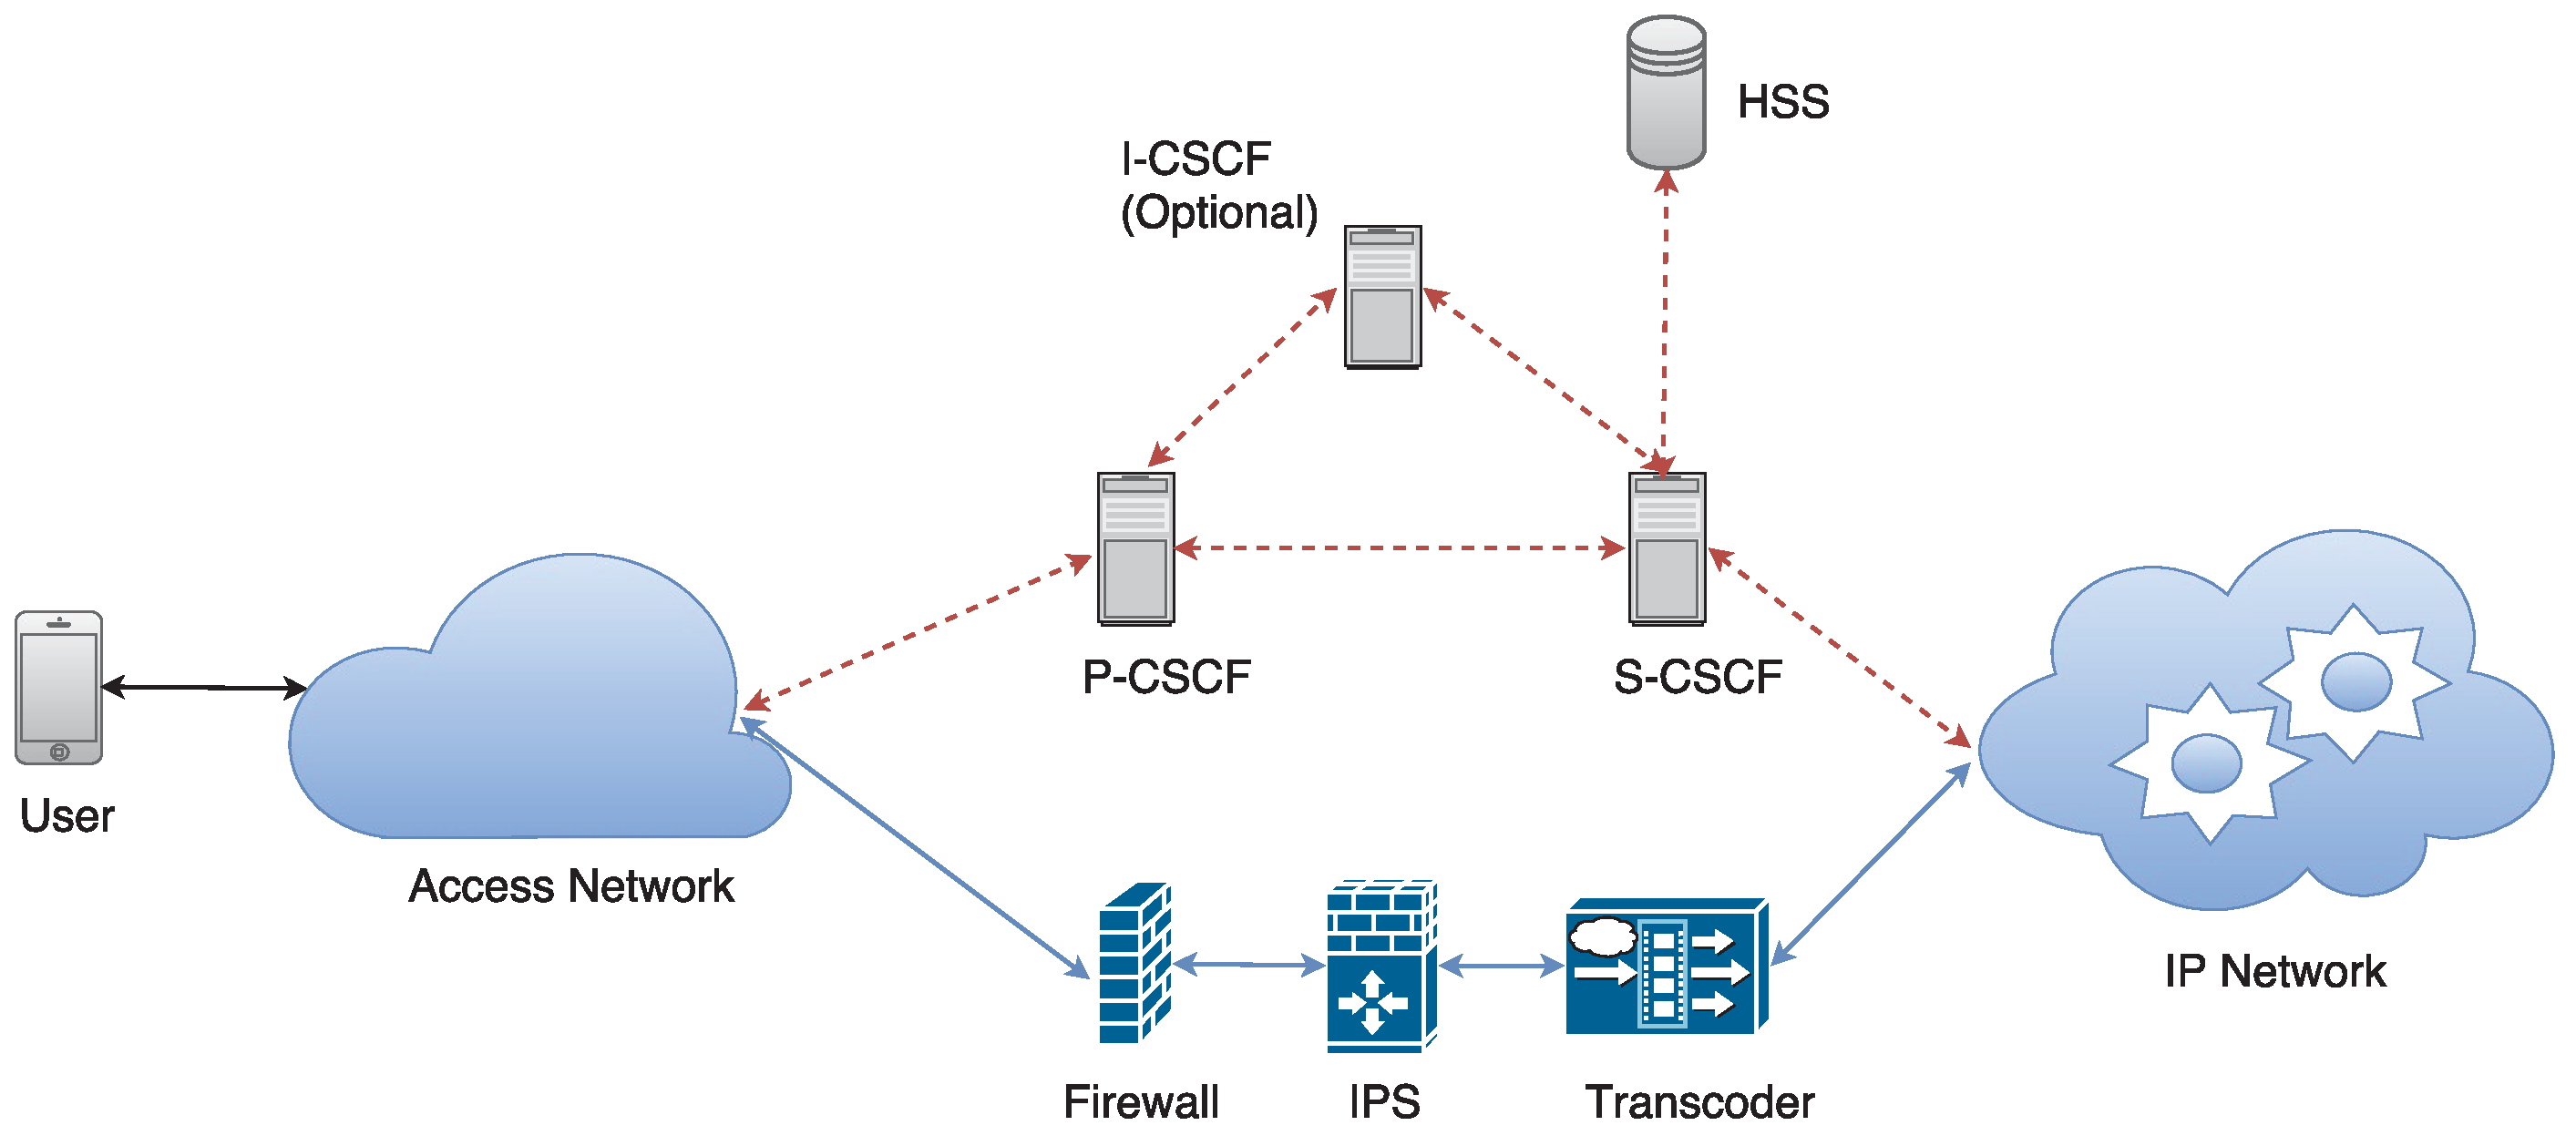
\includegraphics[width=1\columnwidth]{chap-scalims/figure/IMS_architecture.eps}
        \caption{IMS: an architectural overview}
        \label{fig:IMS_architecture}
\end{figure}
%\end{comment}

%cut for space
%old
%An IP Multimedia System (IMS) is a core part in 3G/4G telecom networks (e.g., 3GPP, 3GPP2)~\cite{umts}~\cite{lte}, responsible for delivering multimedia services (e.g., voice, video, messaging) over IP networks. IMS is a fully standardized solution for multimedia service delivery in the telecom industry~\cite{3gpp-ims}, as compared to its proprietary alternatives (e.g., Skype, Facetime). It is a complex system consisting of multiple service chains. We investigate two most important service chains as follows. An illustration is given in Fig.~\ref{fig:IMS_architecture}.
%new
An IP Multimedia Subsystem (IMS)~\cite{3gpp-ims} is a core part in 3G/4G telecom networks (e.g., 3GPP, 3GPP2)~\cite{umts}~\cite{lte}, responsible for delivering multimedia services (e.g., voice, video, messaging) over IP networks. It is a complex system consisting of multiple service chains. We investigate two most important service chains as follows. An illustration is given in Fig.~\ref{fig:IMS_architecture}.

$\triangleright$ \noindent\textbf{Control Plane (CP) Service Chain} includes three main network functions, {Proxy-CSCF (P-CSCF)}, {Interrogating-CSCF (I-CSCF)}, and {Serving-CSCF (S-CSCF)}, %collectively called Call Session Control Function (CSCF),
 which collectively handle user registration, user authentication and call setup. These network functions rely on the Session Initiation Protocol (SIP)~\cite{sip} to interoperate with users of the IMS system. Users can only contact with P-CSCF, which acts as a relay point between users and S-CSCF. Since I-CSCF acts as a middleman that forwards SIP messages between P-CSCF and S-CSCF, real-world implementation sometimes merges I-CSCF into S-CSCF as in \cite{project-clearwater} to simplify the structure of the IMS control plane service chain, making I-CSCF optional. S-CSCF %is the pivot on the control plane. It
  dispatches SIP messages to their final destinations and constantly queries an external storage server called Home Subscriber Server (HSS), which is a database that contains identities of the users. We consider the control plane service chain $\text{P-CSCF} \rightarrow \text{S-CSCF} \rightarrow \text{P-CSCF}$ in \textit{ScalIMS}. % scales the simplified control plane service chain, which has the form of $\text{P-CSCF} \rightarrow \text{S-CSCF} \rightarrow \text{P-CSCF}$.


\begin{comment}
\vspace{-3mm}
\begin{table}[!h]
        \small
        \begin{center}
        \begin{tabular}{p{0.15\linewidth}|p{0.7\linewidth}}
                %\hline
                %NF  & Description\\
                \hline
                P-CSCF & Point of attachment of a user to the IMS. Assigned to user and remains unchanged all time.\\
                \hline
                I-CSCF & Optional for security reason, forwards SIP request or response to the S-CSCF.\\
                \hline
                S-CSCF & Handles SIP message with the help of HSS, and binds the user IP address and the SIP address.\\
                \hline
        \end{tabular}
       % \caption{Network functions for the IMS control plane}
       % \label{tab:control-plane}

        \end{center}
\end{table}
\end{comment}

$\triangleright$ \noindent\textbf{Data Plane (DP) Service Chain} contains a sequence of network functions that the actual multimedia traffic between users traverses, for security (e.g., firewall, deep packet inspection, intrusion detection), connectivity (e.g., NAT, IPv4-to-IPv6 conversion), quality of service (e.g., traffic shaping, rate limiting, ToS/DSCP bit setting), and media processing (e.g., transcoding). While 3GPP has standardized the IMS control plane for interoperability reasons, the exact set of deployed network functions for the data plane varies per operator.


The two service chains collectively handle two important procedures of the IMS system, which are user registration and call setup. %User registration is performed through a SIP REGISTRATION transaction over the control plane.
To make a call, a user first registers his IP address to the IMS by initiating a SIP REGISTRATION transaction over the CP. When the registration is done, S-CSCF temporarily stores the binding between the identity of the user and the P-CSCF instance connected to the user for future calls. To setup a call between a caller and a callee, the caller initiates a SIP INVITE transaction to the IMS, specifying the identify of the callee. S-CSCF uses the binding saved during user registration to retrieve the P-CSCF instance that the callee connects to and sends the message to the P-CSCF instance, which forwards to the callee. After the callee responds, a call is successfully set up. Subsequent media flows between the caller and the callee are routed through DP service chain. When the call is finished, a SIP BYE transaction between the caller and the callee is carried out to close the call over the CP.

%A good NFV management system should effectively scales both the control and data plane service chains of the IMS system. %Since the operation of these two service chains are coupled together through SIP protocol, \textit{ScalIMS} uses a novel method based on flow tagging to effectively scale these two service chains.

\subsection{Related Work}

%In recent years, researchers have pay great attention to NFV technology. By running VNF softwares in virtual machines on computing clusters~\cite{palkar2015e2} or on cloud~\cite{sherry2012making}~\cite{lan2016embark}, service providers could be freed from managing complicated hardware network functions and deploy service chains at ease.

%Performance and scalability of using VNFs in the place of hardware middleboxes have been the focuses of investigation in the existing literature on NFV.

%\noindent \textbf{Performance.}
Running VNF software (e.g., DP packet processing software) on VMs incurs significant context switching cost~\cite{rizzo2013speeding}, limiting the maximum throughput of a VNF. To solve this problem, ClickOS~\cite{martins2014clickos} maps packets directly from NIC receive queues to a shared memory region, and fetch packets directly from that shared memory region~\cite{dpdk}, which greatly improve packet processing throughput. However, this approach completely by-passes the existing kernel networking stack, unable to support VNFs (e.g., S-CSCF and P-CSCF used by IMS system) that use the traditional TCP/IP stack. %
%lose flexibility for network programability (i.e. SDN~\cite{mckeown2008openflow} functionality provided by OpenvSwitch~\cite{pfaff2015design}). On the other hand, some control-plane VNFs (e.g., P-CSCF and S-CSCF as in the Clearwater Project~\cite{project-clearwater}) function well enough on existing network stacks as they are application-level software. If enough scalability is given, existing network stacks could still be used to build NFV service chains.

%\noindent \textbf{Scalability.}
Scaling of service chains has been investigated in a single server, a computing cluster or a datacenter. CoMB~\cite{sekar2012design} focus on scaling VNFs in a single server, %for better performance. %Even though their implementations achieve good performance, but it lacks generality and flexibility.
 by designing customized architecture to unify VNFs inside a single server. % and they can not be cannot be seemlessly integrated into existing SDN framework.
 %E2~\cite{palkar2015e2}, Stratos~\cite{gember2012stratos} and Slick~\cite{anwer2015programming} study scaling of VNFs in a single SDN-enabled datacenter.
 E2~\cite{palkar2015e2} scales VNF service chains in a single datacenter, %scales VNF instances  within a computing cluster connected through SDN enabled switches through
 exploiting high-performance inter-VNF data paths through SDN-enabled switches. % it has its own high performance inter-VNF datapath.
Stratos~\cite{gember2012stratos} %scales VNF instances by
 jointly consider VNF placement and flow distribution within a datacenter, using on-demand VNF provisioning and VM migration to mitigate hotspots.

%To our knowledge, there do not exist NFV management frameworks that scale VNF service chains across geo-distributed datacenters. % while \textit{ScalIMS} concentrates on scaling NFV service chains across datacenters.
The management systems mentioned above cannot be directly extended to the multi-datacenter setting. One primary reason is that SDN controllers~\cite{mckeown2008openflow} are extensively used in these systems to facilitate routing, scaling and load-balancing within a datacenter. However, SDN controllers are rarely available in the WAN, except for among datacenters of a few large providers such as Google~\cite{jain2013b4} and Microsoft~\cite{hong2013achieving}.
%\chuan{change this reference to B4 or SWAN}. %It is extremely hard for a SDN controller to set up flows on other datacenters, which incurs too much delay and hurts flow performance. One possible approach is to deploy one SDN-enabled management system in each datacenter, but there is no existing work on coordinating the behavior of such independent scaling systems, needed for deploying and scaling geo-distributed service chains. %However, scaling systems on different datacenters need to agree on complicated task such as coordinated VNF instance provision and collective flow routing. And all these problems call for an efficient design of a multi-datacenter scaling system.
%A new management system is in need, that efficiently coordinates service chain deployment and scaling, as well as flow routing, across multiple data centers.
 \textit{ScalIMS} is a NFV management system that efficiently coordinates service chain deployment and scaling, as well as flow routing, across multiple data centers. \textit{ScalIMS} uses similar methodologies as in~\cite{palkar2015e2} and \cite{gember2012stratos} when scaling NFV service chains within a datacenter, but adopts a novel distributed flow routing approach and a proactive scaling strategy to scale NFV service chains across multiple datacenters.

Similar with \textit{ScalIMS}, Klein \cite{qazi2016klein} also scales NFV service chains across multiple datacenters. However, it focuses on scaling EPC system \cite{epc} and does not use a hybrid scaling strategy as \textit{ScalIMS} does. Ren et al. \cite{ren2016dynamic} propose a VNF dynamic auto scaling algorithm for 5G networks, but it lacks a real-world implementation when compared to \textit{ScalIMS}.

\section{Challenges and Design Highlights} \label{sec:scalims-motivation}

%\noindent \textbf{Motivation.}
%The key motivation of this study is the fact that there are no NFV scaling systems designed to operate under a multi-datacenter environment, given the following new challenges compared with scaling service chains within a single datacenter.
\textit{ScalIMS} aims to address the following challenges, that arise when scaling service chains over multiple datacenters.

{\em First, deciding service chain paths}, as determined by the datacenters where instances of VNFs in a service chain should be deployed. The service chain path critically decides service quality of user traffic along the chain.
For instance, a traffic flow sent by a user of the IMS system to another user may have two optional paths. The first path traverses a sequence of datacenters $(a, c)$ while the second path traverses datacenters $(a, b, c)$. %Due to the triangle inequality which is a common phenomena in computer network \cite{wang2007towards}, it is possible that the accumulated delay on the second path is way smaller than that on the first path.
The end-to-end delays on the two paths may vary over time. A multi-datacenter NFV scaling system should constantly update the service chain paths, so that a good service quality can be guaranteed for user traffic at all time.
%In Fig.~\ref{fig:system-overview}(a), the flow %traffic of IMS system user can go through either one of the two service chain paths (containing two VNFs each).The lower path leads to a 50ms end-to-end delay while the upper one 100ms.


{\em Second, deciding scaling in/out of network functions}, i.e., adding/removing instances of each VNF upon traffic rise/drop. This decision is coupled with service chain path selection in the multi-datacenter setting. If a service chain path is  overloaded, instead of launching new VNF instances on the same datacenters, the system may search for available VNF instances on other datacenters, and set up new service chain paths using those instances. %This need stands out from the existing studies dealing with a single datacenter, where scaling is achieved through launching new VNF instances only.

{\em Third, distributed flow routing}. %Using SDN to control flow routing in a data center is a common approach adopted by the existing scaling systems. However,
When a service chain path traverses multiple datacenters, it is difficult for a single controller to control the end-to-end route. % due to the lack of support for SDN-like mechanisms over the WAN.
 When multiple SDN controllers are employed in different datacenters, they should work in coordination on constant updates of service chain paths, and correctly route user traffic towards destinations.

%\noindent\textbf{Highlights of {\em ScalIMS}.}
We make the following design decisions in \textit{ScalIMS}. A functional overview of \textit{ScalIMS} is given in Fig.~\ref{fig:system-overview}.

\begin{figure}[!h]
      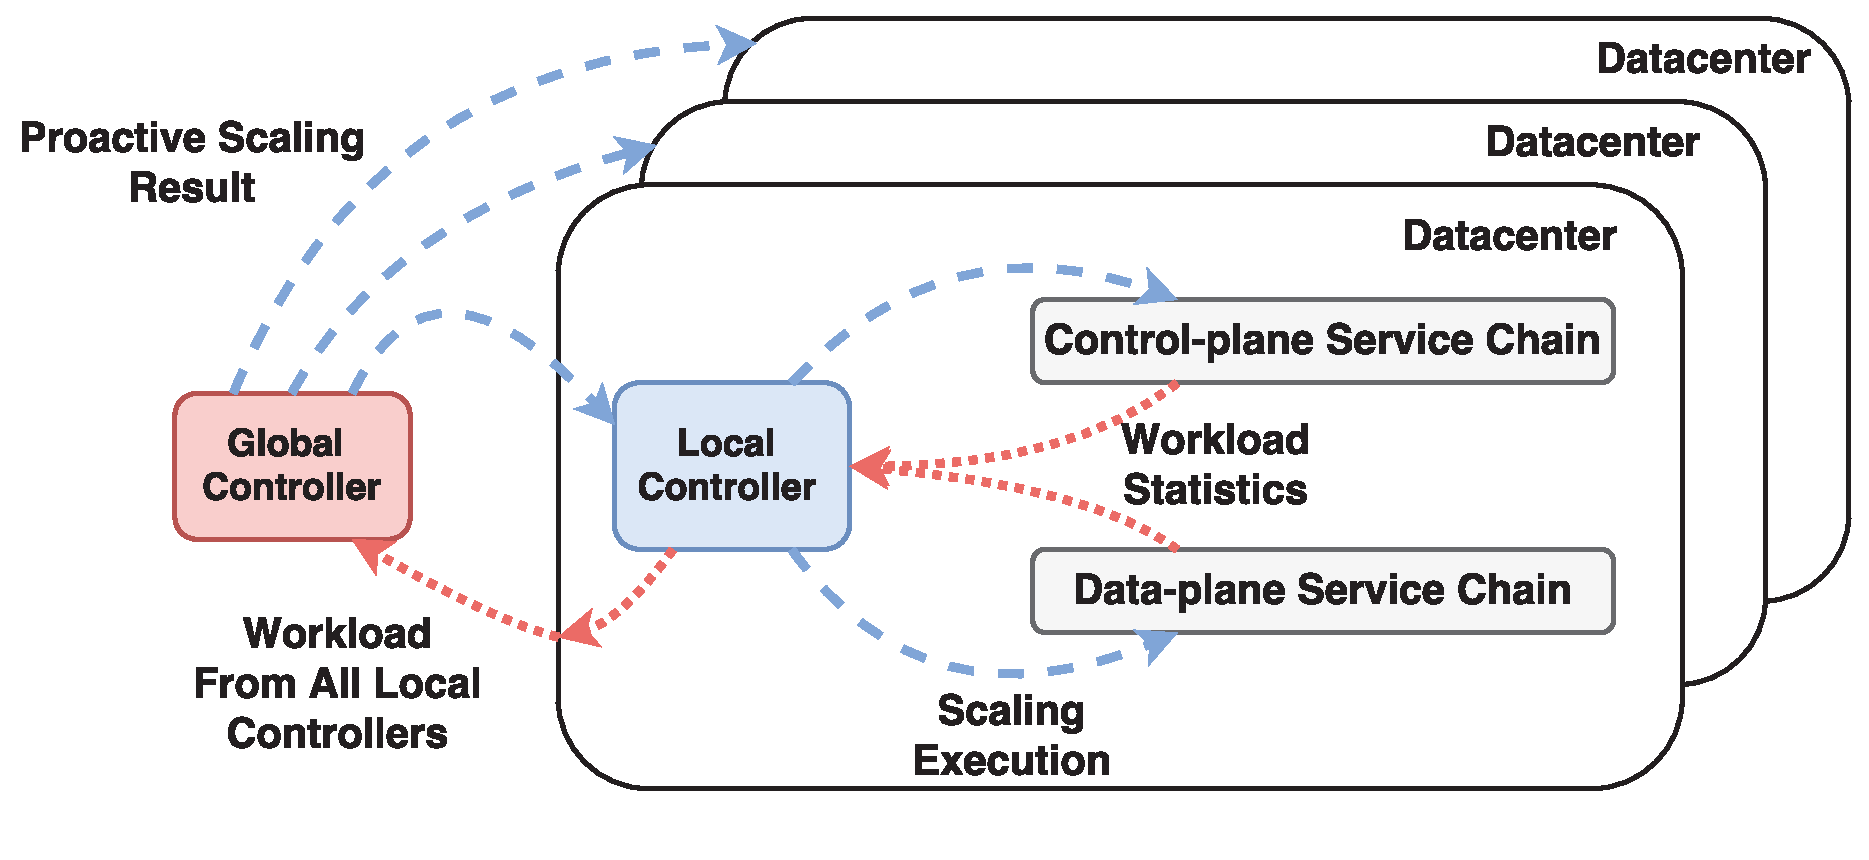
\includegraphics[width=\columnwidth]{chap-scalims/figure/scalims-overall-arch.eps}
    \caption{Functional overview of \textit{ScalIMS}}%: an overview
    \label{fig:system-overview}
\end{figure}

$\triangleright$ We adopt a hybrid scaling strategy, that combines proactive scaling and reactive scaling for both CP and DP service chains. We divide the system time into \textit{scaling intervals}. At the end of each scaling interval, proactive scaling is invoked, which takes as input the predicted workload along each service chain, inter-datacenter latencies and the current VNF deployment (the numbers of instances of each VNF on each datacenter), and generates decisions on VNF scaling and service chain path deployment with bounded end-to-end delay simultaneously for the next scaling interval. Reactive scaling produces scaling decisions of each VNF based on runtime statistics of each instance within each data center. It compensates for the inaccuracy of workload prediction with proactive scaling, improving system performance under unpredicted traffic rate changes.


$\triangleright$ \textit{ScalIMS} enables a synergy of global and local controllers, to best execute the hybrid scaling strategy. The global controller runs on a standalone server. The local controllers are SDN controllers in each data center. For proactive scaling, the global controller coordinates with all local controllers: it collects statistics from each local controller, including CPU/memory usage and network traffic volume, runs the proactive scaling algorithm, generates scaling/deployment decisions, and broadcasts the decisions to local controllers. Each local controller executes the received decisions by launching new VNF instances and adjusting service chain paths. For reactive scaling, a local controller collects runtime statistics from each VNF instance running in its datacenter, and produces local, reactive scaling decision. For flow routing, a local controller uses flow tags and service chain paths received from the global controller to determine the VNF instances that a flow should traverse within its datacenter and be dispatched to in other datacenters.


%cut for space
%$\triangleright$ We bound the end-to-end delays on service chain paths to guarantee good end-to-end performance of flows. We make some design decisions specifically tailored for an IMS system, {\em e.g.}, saving address information carried in the SIP messages on the local controllers to facilitate distributed data-plane flow routing. Similar design philosophies can nevertheless be applied in other geo-distributed NFV systems as well.

$\triangleright$ The architecture of \textit{ScalIMS} follows ETSI NFV MANO framework \cite{nfvmano}, where the global controller closely resembles the NFV orchestrator and the local controller works as both VNF manager and virtual infrastructure manager. Though \textit{ScalIMS} is designed for IMS systems, it can be easily adapted to handle other service chain systems, which provide user inter-connection services with users distributed over a large geographical span. For instance, \textit{ScalIMS} can be adapted to manage the virtualized service chains in Evolved Packet Core (EPC) in 4G LTE network \cite{epc}, by augmenting the CP service chain of EPC with an edge proxy that simulates the functionality of P-CSCF of IMS.

\section{Scaling of Control Plane Service Chain}
\label{sec:scalims-cp}
We first present the detailed design of \textit{ScalIMS} in deployment and scaling of the control plane (CP) service chain. %We start by discussing the scaling strategy used by CP service chain. The proactive scaling is governed by a proactive scaling protocol, whereas the reactive scaling is controlled by overload detection through runtime statistics. The proactive and reactive scaling of CP service chain are generic enough such that the DP service chain uses a similar scaling strategy with CP service chain with only minor difference. This section then presents how SIP messages are transmitted and manipulated on the CP service chain, so that data plane media flows could be routed over correct paths.

\subsection{Deployment and Entry Datacenter Binding} \label{System-Design}

%\subsubsection{Fixed CP Service Chain Placement}
The CP service chain consists of P-CSCF and S-CSCF. We use a fixed placement strategy by deploying P-CSCF instances on every datacenter and S-CSCF instances on a fixed selected datacenter, such that the delay between the datacenter where we place S-CSCF instances and other datacenters falls within an acceptable range (the acceptable SIP transaction completion time is typically 250ms).

%cut for space
%old
%The rationale behind such a fixed placement strategy is the following. S-CSCF instances constantly query the HSS database for user information, and they are usually built as a stateless network function by storing user location information (a temporary mapping between user name and user registration IP address) in a memcached cluster \cite{project-clearwater}. The stateless design improves load balancing among S-CSCF instances, but also implies that even if we spread S-CSCF instances over different datacenters, each S-CSCF instance still needs to access a central HSS server and a memcached cluster to process most of the SIP transactions. This fact urges us to place S-CSCF instances together with the HSS server and memcached cluster in the same selected datacenter. Since P-CSCF instances act as relay points for user flows to access S-CSCF instances, it is desirable to place P-CSCF instances on every datacenter, to facilitate user's access to a P-CSCF instance on the closest datacenter. This fixed placement strategy also simplifies the routing of SIP messages along the CP service chain. % and decisions on the number of CP VNF instances to be deployed in each datacenter.
%new
The rationale behind such a fixed placement strategy is the following. Even if we spread S-CSCF instances over different datacenters, each S-CSCF instance still needs to access a central HSS server and a memcached cluster to process most of the SIP transactions. This fact urges us to place S-CSCF instances together with the HSS server and memcached cluster in the same selected datacenter. Since P-CSCF instances act as relay points for user flows to access S-CSCF instances, it is desirable to place P-CSCF instances on every datacenter, to facilitate users' access to a P-CSCF instance on the closest datacenter. This fixed placement strategy also simplifies the routing of SIP messages along the CP service chain. % and decisions on the number of CP VNF instances to be deployed in each datacenter.

%\subsubsection{Entry Datacenter Binding}

\textit{ScalIMS} binds each user to the nearest datacenter according to his current geographical location, which is referred to as the user's {\em entry datacenter}. A user's CP and DP traffic can only enter and depart from the respective service chains from his entry datacenter. Such a datacenter binding is a natural design choice as each user should be pinned to a unique P-CSCF instance on a specific datacenter when he uses the IMS \cite{3gpp-ims}. %Choosing the geographically nearest datacenter decreases the possibility that the user experiences a large end-to-end delay between him and the entry datacenter.

To implement entry datacenter binding, a DNS server is maintained in \textit{ScalIMS}. When a user queries the IP address of an available P-CSCF instance by sending out a DNS request, the DNS server maps the user's IP address contained in the DNS request to a geographical location by querying an IP-location database ({\em e.g.}, IP location finder~\cite{iplocation}), referred to as the {\em location service}, and then assigns a datacenter that is closest to the user's current location as his entry datacenter.

%\subsubsection{Entry-exit Datacenter Pair}

When a call is initiated between user $a$ and user $b$, user $b$'s entry datacenter is also referred to as user $a$'s {\em exit datacenter}. In \textit{ScalIMS}, each pair of datacenters may form an entry-exit datacenter pair. CP workload and DP workload between each entry-exit datacenter pair are maintained in \textit{ScalIMS}, which are the aggregate rates of traffic that callers associated with an entry datacenter send to callees bound to the exit datacenter, along the CP service chain and the DP service chain, respectively. The traffic rates among entry-exit datacenter pairs are used for traffic prediction and VNF instance provision.

\subsection{Proactive Scaling}
\label{sec:CP_proactivescale}

\begin{figure}[h]
        \centering
        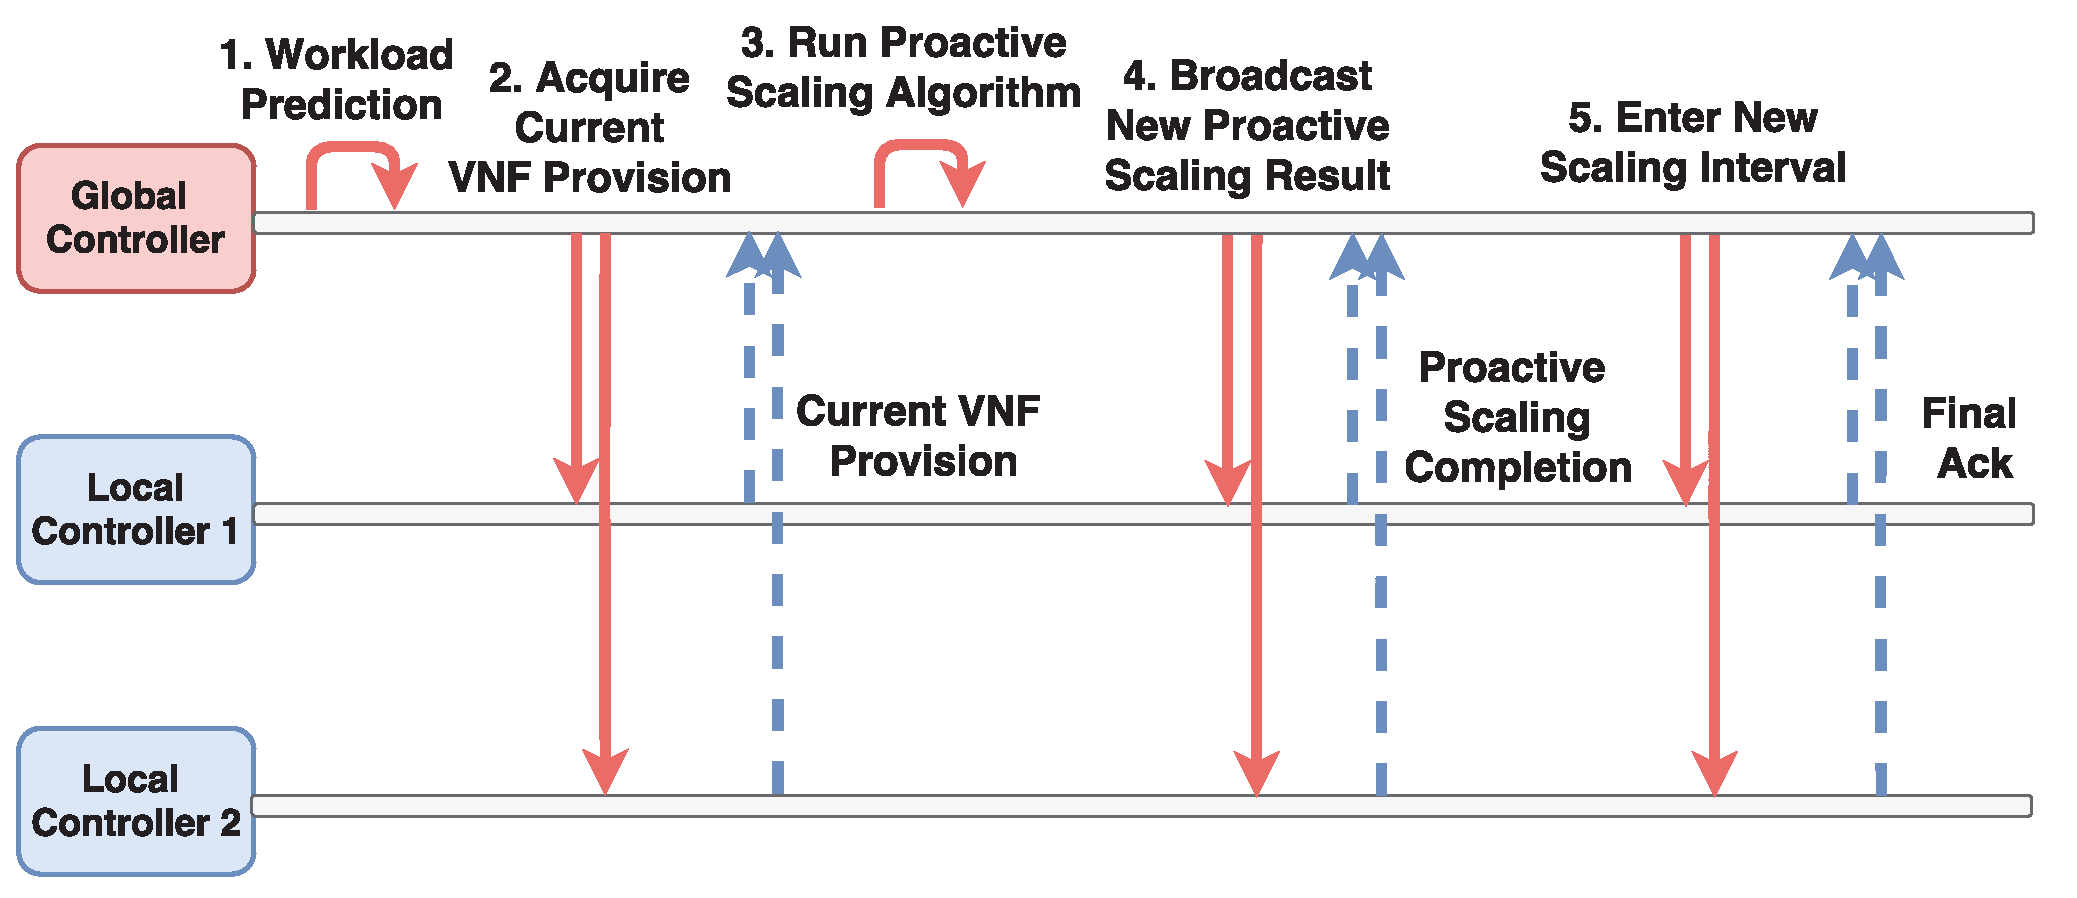
\includegraphics[width=1\columnwidth]{chap-scalims/figure/scaling-work-flow.eps}
        \caption{Proactive scaling protocol.}
        \label{fig:proactive-scaling}
\end{figure}

%cut for space
%old
%Proactive scaling is executed in each scaling interval according to the protocol illustrated in Fig.~\ref{fig:proactive-scaling}. The global controller and each local controller work in a request-response manner. In view of possible message loss, the global controller sets a re-transmision timer that re-transmits a request after 500ms, if no response is received.
%new
Proactive scaling is executed in each scaling interval according to the protocol illustrated in Fig.~\ref{fig:proactive-scaling}.

\noindent\textbf{1. Workload Prediction.}
Workload along a CP service chain is described by the number of SIP transactions carried out between each entry-exit datacenter pair every second. When a SIP transaction finishes, the S-CSCF instance involved uses the location service to determine which entry-exit pair this transaction belongs to (according to the IP addresses of the caller and the callee). Each S-CSCF instance keeps a record of the number of SIP transactions on each entry-exit datacenter pair and reports this number to the local controller in its datacenter every second. The local controller accumulates CP workload for 5 seconds before relaying it to global controller.

At the end of a scaling interval $t$, the global controller predicts the workload $\hat{u}_{t+1}$ in the next scaling interval using historic data in past several intervals (10 as in our experiments), using auto regression~\cite{wood2007black}: $\hat{u}_{t+1} = \mu + \phi(u_t-\mu)$.
%\begin{equation}
%\hat{u}_{t+1} = \mu + \phi(u_t-\mu)
%\end{equation}
%\noindent
Here $\mu$ is the mean of the historic workload values in the past several scaling intervals, $u_t$ is the average CP workload collected in the current interval, and $\phi$ can be decided using the covariance of the historical workload divided by the variance of the historical workload. The workload between each entry-exit datacenter pair is predicted this way.

\noindent\textbf{2. Acquire Current VNF Provision.} The global controller then broadcasts a message to local controllers, asking them to send %information of the current VNF instance provisioning,
 the numbers of instances of each VNF provisioned in the respective datacenter. Upon receiving this request, a local controller knows that proactive scaling computation is on going, stops its reactive scaling process (Sec.~\ref{sec:CP_reactivescale}) so that it does not interfere with proactive scaling, and then sends its current VNF provision information to the global controller.

\noindent\textbf{3. Run Proactive Scaling Alrogihm.} After receiving current VNF deployment from all local controllers, the global controller computes the numbers of P-CSCF and S-CSCF instances to be deployed in each datacenter in the next scaling interval. Since all S-CSCF instances are placed in the same datacenter, the number is decided by dividing the total predicted workload between all pairs of entry-exit datacenters by the processing capacity of S-CSCF. The number of P-CSCF instances to be deployed in a datacenter is computed by dividing the overall predicted workload for the entry-exit datacenter pairs, which use this datacenter as either entry or exit datacenter, by the processing capacity of P-CSCF.

\noindent\textbf{4. Broadcast Proactive Scaling Result.} The global controller then broadcasts the computed numbers to local controllers. A local controller sends a completion message to the global controller, after creating new VNF instances (scale-out) or enqueueing unused VNF instances to the respective buffer queues (scale-in), according to the received numbers.

\noindent\textbf{5. Enter New Scaling Interval.} After the global controller receives completion messages from all local controllers, it broadcasts an ``enter new scaling interval'' message to all local controllers. After receiving this message, a local controller increments its scaling interval index by 1, and shuts down some VNF instances from the head of the buffer queues. Then the local controller sends a final acknowledgement to the global controller. Upon receiving all final acknowledgements, % from all local controllers,
 the global controller increases its scaling interval index by 1.

\textit{Buffer Queue.} In each datacenter, a double-ended buffer queue is maintained to temporarily hold unused VNF instances, with one queue for one type of VNF. When a VNF instance is to be removed, instead of directly shutting it down, the local controller tags it with the index of the current scaling interval, and enqueues it to the tail of the respective buffer queue. Once a VNF instance is enqueued, no more flows will be routed to it. Whenever more instances of a VNF are to be established, if there are available instances in the buffer queue of this VNF, buffered instances will be popped out from the tail of the queue, and transformed back to working instances, to fulfil the demand as much as possible. The purpose is to avoid creating new VNF instances frequently and improve flow loss rate, as the typical VNF creation time can last a few seconds and has a bad influence on flow loss rate. Unused buffered VNF instances are destroyed after $\tau$ scaling intervals ($\tau$ is set to 10 in our implementation), in Step 5 above.
%: when the local controller in the datacenter receives an ``enter new scaling interval message'', it checks from the head of each buffer queue whether an instance has been enqueued $\tau$ intervals ago; if so, the VNF instance at the head will be dequeued. Dequeuing repeats until all unused instances for $\tau$ intervals are cleaned. These dequeued VNF instances gets destroyed by local controller when there's no active traffic on them.
% The local controller will destroy dequeued VNF instances until there's no active traffic on them.

\vspace{-3mm}
\subsection{Reactive Scaling}
\label{sec:CP_reactivescale}

%Duan's new:
%address some problems
An agent running on each VNF instance reports to the local controller runtime statistics of the instance, e.g., CPU usage, memory usage and the number of input packets, in each second. The local controller maintains time series of these statistics for each VNF instance. It decides whether CPU, memory, or network is overloaded during the past several seconds by comparing the respective statistics with a threshold (Sec.~\ref{sec:scalims-evaluation}). If overload is persistently identified for at least two types of statistics ({\em e.g.}, CPU and network usage) for some consecutive time (5 seconds as in our experiments), then that VNF instance is reported as overloaded. We make the decision using two types of statistics in order to eliminate false alarms brought by examining a single statistics. The local controller then avoids routing new traffic flows ({\em i.e.}, new calls) to overloaded instances if there are other available instances. In a datacenter, if the states of a majority of instances of a VNF are ``overloaded'', scale-out is triggered by adding one new instance of that VNF. Note that no scale-in decisions (i.e., removing instances) are made reactively. They are solely handled by the proactive scaling protocol, as it improves system stability during workload fluctuation.
%Because efficient reactive-scale-in requires support of dynamic flow migration \cite{gember2014opennf} to quickly shutdown idle VNF instances, which is hard to implement.

\subsection{Flow Routing on Control Plane}
\label{sec:message-routing-on-control-plane}

When a user connects to the IMS system, he first issues a query to a DNS server, which determines the entry datacenter of this user and obtains the IP address of an available P-CSCF instance (non-overloaded) by querying the local controller of the entry datacenter. A P-CSCF instance learns the IP addresses of several available S-CSCF instances (non overloaded) by querying the local controller of the datacenter hosting S-CSCF instances and distributes its up-stream requests to these S-CSCF instances evenly. It regularly (every 30s in \textit{ScalIMS}) updates the connections to up-stream S-CSCF instances by querying the local controller to obtain an updated view of S-CSCF instances.


%explain how flows are routed in case of P-CSCF and S-CSCF scale-in and scale-out.


%we must state the SIP message manipulation here, as the routing of data plane flows will use these mappings to obtain flow's service chain path
A CP flow for establishment of a call (i.e., a SIP INVITE transaction) runs as follows.
The caller sends out a SIP INVITE message, carrying caller's source IP address, receive port and send port, to the assigned P-CSCF instance.
%A SIP INVITE message carries the caller's source IP address, receive port and send port.
The P-CSCF instance forwards the message to one connected S-CSCF instance.  The
S-CSCF instance queries the HSS database to obtain the P-CSCF instance assigned
to the callee that is saved when callee registers himself, and forwards the SIP
INVITE message to that P-CSCF instance. The P-CSCF instance assigned to the
callee modifies the source IP field in the message to an IP address located on
the callee's entry datacenter, so that the callee can learn an IP address
located on callee's entry datacenter. The P-CSCF instance then sends the
modified SIP INVITE message to the callee.  The callee responds with a SIP OK
message, going through the same service chain in the reversed direction. When
the SIP OK message passes through caller's entry datacenter, the P-CSCF instance
modifies source IP field in the message to an IP address located on caller's
entry datacenter as well. When such a SIP INVITE transaction ends, the
caller and the callee use the learned IP addresses as the destination IP addresses of the DP media flows and send their media flows to their entry datacenters, from where the media flows enter the DP service chain.

%The content of these two messages are modified by the P-CSCF instance in order for the caller/callee to learn a destination IP address on his entry datacenter.  When a SIP INVITE message passes through callee's entry datacenter, the source IP field is modified to an IP address located on the callee's entry datacenter, so that the callee learns about a destination IP address located on callee's entry datacenter. A similar process is applied to SIP OK message when the message passes through caller's entry datacenter as well.


Besides SIP message modification, a P-CSCF instance sends two mappings (Table~\ref{mappings}) to its local controller after it has received the SIP OK message. The local controller saves these mappings for use when processing the DP flows (Sec.~\ref{sec:scalims-dp}). %The saved mapping differs depending on whether the P-CSCF instance is on caller's or callee's entry datacenter.



\begin{table}[t]
	\caption{Mappings saved on local controller}% of entry datacenter}
	\label{mappings}
\centering
\resizebox{\columnwidth}{!}{%
\begin{tabular}{| l |p{0.75\columnwidth}|}
\hline
\multirow{2}{*}{\begin{tabular}[c]{@{}l@{}}Controller on\\ Caller Entry DC\end{tabular}} & 1. (caller IP, caller send port)$\rightarrow$(callee IP)                   \\ \cline{2-2}
                                                                                & 2. (callee IP, callee send port)$\rightarrow$(an IP on caller's entry datacenter, caller IP, caller receive port) \\ \hline
\multirow{2}{*}{\begin{tabular}[c]{@{}l@{}}Controller on \\ Callee Entry DC \end{tabular}} & 3. (callee IP, callee send port)$\rightarrow$(caller IP)                   \\ \cline{2-2}
                                                                                & 4. (caller IP, caller send port)$\rightarrow$(an IP on callee's entry datacenter, callee IP, callee receive port) \\ \hline
\end{tabular}
}
\end{table}

\vspace{-3mm}
\section{Scaling of Data Plane Service Chain}
\label{sec:scalims-dp}

The DP service chain adopts the same reactive scaling mechanism as discussed in Sec.~\ref{sec:CP_reactivescale}. For proactive scaling, the same steps %proactive scaling protocol
as shown in Fig.~\ref{fig:proactive-scaling} is followed, with the following differences.

%Duan's new:
{\em First}, the proactive scaling algorithm for DP service chain, running in Step 3 in Fig.~\ref{fig:proactive-scaling}, not only decides how VNF instances are provisioned in each datacenter, but also updates the service chain path (Sec.~\ref{sec:dp-service-chain-path}) between each entry-exit datacenter pair. The new proactive scaling algorithm will be discussed in Sec.~\ref{sec:dp-proactive-scaling-alg}.

{\em Second}, workload along a DP service chain is described as the number of packets transmitted over each entry-exit datacenter pair every second. The local controller acquires input DP workload using workload measuring OpenFlow rules installed on the SDN switch at each datacenter, and reports DP workload measurements to the global controller every second. Local controllers also constantly measure inter-datacenter delays through a ping test among each other, and report the ping delays to the global controller every second. In Step 1 of Fig.~\ref{fig:proactive-scaling}, not only workload but also delays between datacenters are predicted for the next interval, using the same approach as discussed in Sec.~\ref{sec:CP_proactivescale}.

{\em Next}, each local controller also acts as the SDN controller to manage DP flow routing within the respective datacenter. When a local controller receives DP proactive scaling results in Step 4 of Fig.~\ref{fig:proactive-scaling}, it immediately adds/removes DP VNF instances accordingly, but saves the new DP service chain paths and uses them for routing only after receiving the ``enter new scaling interval'' message in Step 5 of Fig.~\ref{fig:proactive-scaling} (Sec.~\ref{sec:flow-routing-on-dp}).
%This 2-stage update is used to guarantee consistency for distributed flow routing (see Sec.~\ref{Inconsistency}).

%DP workload is described by the number of the packet sent over each entry-exit datacenter pair every second. Local controller acquires input DP workload by reading workload measuring OpenFlow rules installed on the entry switch (see Sec.\ref{sec:flow-routing-on-dp}). DP workload is reported to the global controller every second. DP proactive scaling algorithm also needs inter-datacenter delay prediction to update service chain paths. It is measured by each local controller through a ping test to every other local controllers and the result is reported to global controller every second.

\subsection{DP Service Chain Path}
\label{sec:dp-service-chain-path}

%Since the configuration of DP service chain is not specified in the 3GPP specification \cite{3gpp-ims}, \textit{ScalIMS} seeks to find out a generic algorithm that can be applied to any service chain configuration. Under a single-datacenter scenario, the service chain only consists of a list of VNFs that the traffic flow must traverse in sequence. But under the multi-datacenter scenario that \textit{ScalIMS} operates, it is important to consider on which datacenter the traffic flow should go through a specific VNF on the service chain, so that resources on different datacenters could be utilized with more efficiency.

% We refer to VNFs in a DP service chain as {\em stages} of the chain and index them following the order of the VNFs in the chain. For example, DP service chain used in \textit{ScalIMS} contains firewall (stage 1), IDS (stage 2) and transcoder (stage 3). Since \textit{ScalIMS} manages multiple datacenters, we define a {\em service chain path} between each pair of entry-exit datacenters to be a path of datacenters. For a service chain with $m$ stages, a service chain path contains $m+2$ datacenters. The $0$th and $m+1$th datacenter are entry datacenter and exit datacenter of the entry-exit datacenter pair associated with the service chain path. The $i$th datacenter ($i=1, ..., m$) hosts instances of stage $i$ VNF in the service chain. Stage $1$ and stage $m$ could be hosted on other datacenters other than entry and exit datacenter. For example, a service chain path of $(0, 0, 1, 1, 2)$ shows that datacenter 0 is the entry datacenter, stage 1 to stage 3 of the service chain are hosted on datacenters 0, 1, and 1, respectively, and the exit datacenter is datacenter 2. Note that even if instances of a VNF may be deployed on different datacenters, we maintain only one service chain path for each service chain between each entry-exit datacenter pair in each single scaling interval, for path computation efficiency.

\textit{ScalIMS} employs one DP service chain path for all the DP media flows sharing the same entry-exit datacenter pair. A service chain path is a sequence of datacenters $l[0],\ldots,l[m+1]$, where $l[0]$ and $l[m+1]$ are the indexes of the entry datacenter and exit datacenter, respectively, and $l[i], 1\le i\le m$, is the index of the datacenter hosting the $i$th VNF in a $m$-stage service chain.
%each hosting one VNF in the service chain, ordered in the sequence of VNFs in the service chain, plus the entry and exit data centers. %A service chain path indicates a specific VNF on the DP service chain should hosted on which datacenter for all the DP media flows sharing the same entry-exit datacenter pair.
For example, the DP service chain in our implementation of \textit{ScalIMS} is ``firewall (stage 1)$\rightarrow$IDS (stage 2) $\rightarrow$ transcoder (stage 3)'', and a service chain path is a sequence of $5$ datacenters. The DP proactive scaling algorithm constantly adjusts the service chain path for each entry-exit datacenter pair, to efficiently utilize deployed VNF instances.

The definition of service chain path augments an actual service chain with a virtual entry stage $0$ and a virtual exit stage $m+1$. These two stages are forced to be placed on the entry and exit datacenter respectively, so that entry and exit datacenters are guaranteed to be connected together. The two virtual stages have infinite capacities.

% and guarantee a bounded end-to-end delay.

%We refer to VNFs in a DP service chain as {\em stages} of the chain and index them following the order of the VNFs on the chain. For example, DP service chain used in \textit{ScalIMS} contains firewall (stage 1), IDS (stage 2) and transcoder (stage 3). For a DP service chain that consists of $m$ stages, a service chain path is defined as a list $l[0...m+1]$ with length $m+2$. Each list item in $l$ is the index of a datacenter controlled by \textit{ScalIMS}. In particular, $l[0]$ and $l[m+1]$ are the indexes of the entry datacenter and exit datacenter, respectively. $l[i], 1 \leq i \leq m$ indicates that datacenter with index $l[i]$ should host stage $i$ VNF for all the DP media flows that share the same entry-exit datacenter pair $(l[0], l[m+1])$.

%The definition of service chain path $l[0...m+1]$ introduces two virtual stages to an actual service chain with $m$ stages, which are the virtual entry stage $0$ and virtual exit stage $m+1$. The virtual entry stage $0$ and virtual exit stage $m+1$ are forced to be placed on the entry datacenter and exit datacenter respectively. Such a representation guarantees that the resulted service chain path connects the entry and exit datacenter together.


Each service chain path should satisfy two conditions. (i) Looplessness: if datacenter $i$ hosts both stages $x$ and $y$, $x<y$ on the service chain, then datacenter $i$ must host stage $z$, where $x<z<y$ too; otherwise, a routing loop is created on the inter-datacenter network, which increases end-to-end delay and wastes important inter-datacenetr network bandwidth. There is no need for \textit{ScalIMS} to tackle routing loops inside a datacenter, as routing loops inside datacentres are not common and can be resolved by method described in \cite{stephens2012past}. (ii) Bounded end-to-end delay between the entry datacenter and the exit datacenter along the service chain path, by a pre-defined threshold. %, otherwise DP media flows using this service chain path may experience unexpected high round-trip-time.

\subsection{DP Proactive Scaling Algorithm}
\label{sec:dp-proactive-scaling-alg}


\begin{algorithm}[!t]
\KwIn{Predicted delay between each datacenter pair, predicted workload of each entry-exit datacenter pair, current VNF deployment, current service chain paths}
\KwOut{New VNF instance provisioning, new service chain paths}
{Compute total available processing capacity of instances of each VNF in each datacenter}\;
\ForEach{entry-exit datacenter pair $p$, $p.entry \neq p.exit$} {% in workload prediction matrix} {
 	\If{there is enough VNF capacity on $p$'s current service chain path and the end-to-end delay threshold is not violated along $p$'s current path}{
		{use $p$'s current service chain path as new path and reduce available processing capacities of VNFs on $p$'s new path by predicted workload}\;
	}
}
\ForEach{$p$, $p.entry \neq p.exit$ $\&\&$ $p$'s new service chain path has not been determined} {
 	{compute a new path for $p$ using Alg.~\ref{algo:pc}}\;
	\If{there is not enough capacity on $p$'s new path}{
		\ForEach{datacenter $d$ on the new path}{
		{create $\lceil \max\{0,Q-Q'\}/C \rceil$ new instances of the VNF that datacenter $d$ hosts for $p$, where $Q$ is $p$'s predicted workload, $Q'$ is the total capacity of the VNF in $d$ and $C$ is per-instance processing capacity of that VNF}\; %where sufficient to serve $p$'s predicted workload
	{reduce available processing capacities of instances of the VNF in $d$ by predicted workload}\;
	}
}
}
\ForEach{$p$, $p.entry = p.exit$} {
 	{use $p$'s current service chain path as new path, and carry out same actions as in line 7-10 }\;
	%\If{there is not enough capacity on $p$'s new path}{
	%	{scale out by creating new VNF instances sufficient to serve $p$'s predicted workload}\;
	%}
	%{reduct available processing capacities of VNFs on $p$'s new path by predicted workload}\;
	}
{scale in by enqueuing un-used VNF instances to the respective buffer queues}\;
\caption{DP Proactive Scaling Algorithm}
\label{algo:dpalg}
\end{algorithm}

%version 1
The DP proactive scaling algorithm is given in Alg.~\ref{algo:dpalg}, which computes a new service chain path for the next scaling interval, for each entry-exit datacenter pair. % performs scale-out in case of a shortage of VNF processing capacities and reduces the available processing capacities on the service chain path by the predicted workload (lines 1-14).
The algorithm first tries to reuse as many existing service chain paths as possible based on the current VNF provisioning, as long as the capacity is sufficient to handle predicted workload and the end-to-end delay threshold is still guaranteed (lines 2-4). In case that an existing service chain path can not be reused, a new service chain path is computed using Alg.~\ref{algo:pc} (lines 5-6), and scale-out is carried out if there is a shortage of VNF processing capacities (lines 7-10). For an entry-exit datacenter pair $p$ where the entry and exit datacenters are the same, the entire service chain path of $p$ is always deployed in this datacenter (lines 11-12). %The algorithm processes these entry-exit datacenter pairs at last so that the VNF capacity can be utilized more efficiently (lines 10-14).
Finally, scale-in is carried out to enqueue un-used VNF instances into the buffer queue (line 13).


%For an entry-exit datacenter pair $p$, if there is not enough VNF capacity to serve the predicted workload on $p$'s new service chain, $\lceil (Q-Q')/C \rceil$ new VNF instances are created for the respective VNF in the respective datacenter (whose capacity is in shortage), where $Q$ is $p$'s predicted workload, $Q'$ is the total capacity of the VNF in the respective datacenter and $C$ is the processing capacity of each instance of that VNF (lines 7-8).


%In the stage placement algorithm discussed in Sec.~\ref{sec:stage-placement-algorithm}, the virtual entry stage and virtual exit stage both have infinite capacities.
\subsection{Service Chain Path Computation}
\label{sec:pathcomp}


\begin{algorithm}[!t]
\KwIn{Predicted inter-datacenter delays, an entry-exit datacenter pair $p=(entry, exit)$, $p$'s predicted workload, $p$'s current service chain path, current available processing capacities of VNF instances, the service chain of $m$ stages, $n$ datacenters}
\KwOut{$p$'s new service chain path}
{minProvPath = $p$'s current path}\;
\For{$v = 0, ..., exit-1, exit+1, ..., n-1$}{
	{$record[0] = entry$, $record[1] = v$, $record[m+1] = exit$}\;
	\For{$x = 2, ..., m$}{
		{find out datacenter $v_1$ ($v_1 \neq exit$) that has the largest available capacity for stage-$x$ VNF}\;
		{$record[x] = v_1$}\;
  		\If{there is path loop on $record$}{
   			{eliminate loop by adjusting $record$}\;
  		}
		{$path[0, ..., x] = record[0, ..., x]$}\;
		{$path[x+1, ..., m+1] = exit$}\;
		%{$path[x+1, ..., m-1] = exit[x+1, ..., m+1]$}\;
		\If{$path$ leads to a smaller number of new VNF instances to be created for hanlding predicted workload than minProvPath and satisfies end-to-end delay requirement}{
		 minProvPath = path
		}
 	}
	{$path[0]=entry, path[1]=v, path[2, ..., m+1] = exit$}\;
	{check whether $path$ should be assigned to minProvPath as in lines 11-12}\;% and assign it to $minProvPath$ accordingly}\;
}
{$path1[0]=entry, path1[1, ..., m+1] = exit$}\;
{$path2[0, ..., m]=entry, path2[m+1] = exit$}\;
{check whether $path1$ or $path2$ should be assigned to minProvPath as in lines 11-12}\;%, assign $minProvPath$ accordingly}\;
\If{minProvPath violates end-to-end delay requirement}{
 {find out the shortest-delay datacenter path between entry and exit}\;
 {run stage placement algorithm in Alg.~\ref{algo:sp} and assign the identified service chain path to minProvPath}\;
}
\Return{minProvPath}\;
\caption{Service Chain Path Computation}
\label{algo:pc}
\end{algorithm}

\noindent \textbf{Algorithm Overview.} Alg.~\ref{algo:pc} presents the algorithm to compute a good service chain path between a given entry-exit datacenter pair, that aims to minimize the number of new VNF instances to be created %for handling the predicted workload
 while satisfing the end-to-end delay requirement. % (lines 10 $\sim$ 11).
 For a service chain of $m$ VNFs (stages) and $n$ datacenters, exhaustive search to identify such a service chain path incurs $O(m^n)$ running time. Instead, Alg.~\ref{algo:pc} seeks to optimistically find a good path in $O(mn)$ time.

In Alg.~\ref{algo:pc}, the $record$ list retains the service chain path under investigation (line 3). The search starts by looping through all datacenters except the exit datacenter, to decide the one for hosting instances of stage-1 VNF %for use of flows between the input entry-exist pairDuan: I think this is enough
(lines 2-3). For each subsequent VNF in the service chain, a datacenter (except the exit datacenter) with the largest available processing capacity of the respective VNF is chosen (lines 4-6). We might have created a loop in the service chain path. % (see Sec.~\ref{sec:dp-service-chain-path}).
 If so, the loop is eliminated (lines 7-8) using the method to be discussed next. %in Sec.~\ref{sec:loop-elimination}.
 Whenever the datacenter to host stage-$x$ VNF is determined, a candidate path is produced by assuming all the rest VNF stages ($x+1,\ldots, m$) will be hosted in the exit datacenter (lines 9-10). The candidate path is examined by calculating the number of new VNF instances to be created along this path and the end-to-end delay of this path. If the candidate path incurs addition of fewer new VNF instances than the current best candidate path while satisfying end-to-end delay requirement, we retain it in $minProvPath$ (lines 11-12). The algorithm also checks some naive candidate paths that are not generated by the search loop (lines 13-17). Finally, it is possible that all candidate paths found so far fail to satisfy the delay requirement. If so, we compute the shortest end-to-end delay path using a shortest path algorithm, and run the stage placement algorithm in Alg.~\ref{algo:sp}  % Sec.~\ref{sec:stage-placement-algorithm})
  to produce the service chain path (lines 18-20).

\begin{comment}
	Suppose that Alg.~\ref{algo:pc} is finding a service chain path for entry-exit datacenter pair $(1, 5)$ and the DP service chain consists of $3$ stages. During the execution of the algorithm, the {\em record} list contains $(1, 2, 4, tbd, 5)$. It means the algorithm has determined that instances of stage $1$ VNF should be placed on datacenter $2$ and instances of stage $2$ VNF should be placed on datacenter $4$. And the algorithm is going to find out a datacenter for hosting instances of stage $3$ VNF. If datacenter $2$ is selected to host the stage-$3$ VNF, then the {\em record} becomes $(1, 2, 4, 2, 5)$ and a loop is created between datacenters $2$ and $4$.
\end{comment}

\noindent \textbf{Loop Elimination.}
%\label{sec:loop-elimination}
To eliminate a loop in the path introduced in lines 5-6 of Alg.~\ref{algo:pc}, we adjust the {\em record} list following two ways: (i) place all VNF stages involved in the loop on the datacenter at the start of the loop. Suppose the path with loop is $(1, 2, 4, 2, 5)$. It is adjusted to $(1, 2, 2, 2, 5)$, i.e., the datacenter hosting stage $2$ is changed from datacenter $4$ to datacenter $2$. %  Considering the previous example, it means that the record is adjusted to $(1, 2, 2, 2, 5)$ by changing the datacenter hosting stage $2$ from datacenter $4$ to datacenter $2$.
(ii) Choose a new datacenter to replace the datacenter that leads to the loop, which has the second largest available capacity for hosting the respective VNF and will not create another loop. Suppose datacenter $3$ in the above example has the second largest capacity of stage-$3$ VNF. Then the path is adjusted to %datacenter $3$ replaces datacenter $2$ to host stage $3$ VNF, turning {\em record} list into
 $(1, 2, 4, 3, 5)$. The {\em record} list is adjusted in both ways and the two resulting lists are compared. The list requiring fewer new VNF instances is selected.
%Recall that for a service chain with $m$ stages, the service chain path of an entry-exit datacenter pair contains $m+2$ stage, where stage 0 and stage $m+1$ are put on entry and exit datacenter respectively. These 2 stages are virtual stages for delivering traffic and they have infinite capacity.

\begin{algorithm}[!t]
\KwIn{The shortest-delay datacenter path $d[0...k-1]$ as a list of distinct datacenter indices between entry-exit datacenter pair ($d[0], d[k-1]$)
; DP service chain with $m+2$ stages (augmented with virtual entry and exit stage discussed in Sec.~\ref{sec:dp-service-chain-path}) and per-instance capacity $C_j, 0 \leq j \leq m+1$, of stage-$j$ VNF; % The service chain is augmented with a virtual entry stage $0$ and a virtual exit stage $m+1$ with infinite capacity (see Sec.~\ref{sec:dp-service-chain-path}).}
 overall processing capacities $Q'_{i,j}$ of all stage-$j$ VNF instances in datacenter $d[i]$; predicted workload $Q$ for entry-exit datacenter pair $(d[0], d[k-1])$}
\KwOut{service chain path $l[0], \ldots, l[m+1]$ for entry-exit datacenter pair ($d[0], d[k-1]$).}

%\KwMethod{ Solve the dynamic programming problem listed in Eqn. (1) to (5).
%}

{Calculate $N(i,j), \forall i=0,\ldots,k-1, j=0, \ldots, m+1$, as follows:
%\begin{equation}
%0 \leq i \leq n-1, 0 \leq j \leq m+1
%\label{eq1}
%\end{equation}
\begin{equation}
\resizebox{0.95\columnwidth}{!}{
$num(i,j)=
  \begin{cases}
    0,                                        &\text{if $Q'_{i,j} \geq Q$ and $m-j+1 \geq k-i-1$}\\
    \lceil(Q-Q'_{i,j})/C_j\rceil, &\text{if $Q'_{i,j}<Q$ and $m-j+1 \geq k-i-1$}\\
    +\infty,                                &\text{if $m-j+1<k-i-1$}
  \end{cases}$}
 \label{eq6}
\end{equation}
\begin{equation}
N(0, 0) = 0, N(i, 0) = +\infty, i=1,\ldots,k-1 %i \geq 1
\label{eq2}
\end{equation}
\begin{equation}
N(0, j) =  N(0, j-1)+num(0,j), j=1, \ldots, m+1%j \geq 1
\label{eq3}
\end{equation}
\begin{equation}
\begin{aligned}
 N(i, j) = min\{ N(i-1, j-1)+num(i, j), N(i, & j-1) +num(i,j) \}, \\
 i=1,\ldots,k-1, j=1, \ldots, m+1 %i \geq 1~\text{and}~j \geq 1
\end{aligned}
\label{eq5}
\end{equation}
}%\;

%{Calculate the rest of the elements in table $N(i,j)$ using Eqn.~\ref{eq3} to~\ref{eq6}}\;

{Backtrack from $N(k-1, m+1)$ to derive the service chain path $l[0], \ldots, l[m+1]$}\;

\Return{$l[0], \ldots, l[m+1]$}\;

\caption{Stage Placement Algorithm}
\label{algo:sp}
\end{algorithm}

\noindent\textbf{Stage Placement Algorithm.} Alg.~\ref{algo:sp} gives the stage placement algorithm used in line 20 of Alg.~\ref{algo:pc}, which calculates a service chain path, i.e., the sequence of datacenters to host VNF stages on the service chain, that minimizes the number of new VNF instances to be created on the path. %The resulting service chain path must traverse all the datacenters on the datacenter path in sequence without creating a routing loop.

In Alg.~\ref{algo:sp}, $num(i, j)$ is the number of new stage-$j$ VNF instances to be created, if stage $j$ is to be deployed on datacenter $d[i]$. $num(i, j)$ is computed in Eqn.~\ref{eq6} based on the following observation: if datacenter $d[i]$ is chosen to host stage $j$, then the remaining number of yet-to-be-placed stages, $(m+2)-(j+1)$, must be no smaller than the remaining number of datacenters which do not host any stage yet, $k-(i+1)$, as otherwise the resulting service chain is not able to traverse the shortest-delay datacenter path in sequence. %The third condition in Eqn.~(\ref{eq6}) reflects this observation, where as the first two conditions in Eqn.~(\ref{eq6}) are calculated as usual.

$N(i, j)$ is the minimum number of instances of stage $0$ to stage $j$ VNFs, if stage $j$ is to be deployed on datacenter $d[i]$. The computation of $N(i, j)$ is a dynamic programming problem (Eqn.~(\ref{eq2}) to~(\ref{eq5}) in Alg.~\ref{algo:sp}). Eqn.~(\ref{eq2}) to Eqn.~(\ref{eq3}) are base cases, initialized according to the fact that stage $0$ is on the entry datacenter $d[0]$. Eqn.~(\ref{eq5}) is derived based on the following observation: if datacenter $d[i]$ is chosen to host stage $j$, then stage $j-1$ can only be hosted on either datacenter $d[i-1]$ (the previous datacenter on the datacenter path) or datacenter $d[i]$.

%If this observation is violated, then the resulted service chain path may not traverse the datacenter path in sequence. %Based on this observation, $N(i-1,j-1)+num(i,j)$ is the smallest number of newly created VNF instances if stage $j-1$ is hosted on datacenter $d[i-1]$, where as $N(i,j-1)+num(i,j)$ is the smallest number of newly created VNF instances if stage $j-1$ is hosted on datacenter $d[i]$, and $N(i,j)$ is the minimum value among the two.


 %Line 3 of Alg.~\ref{algo:sp} backtracks from $N(n-1, m+1)$ because the virtual exit stage $m+1$ can only be placed on exit datacenter $d[n-1]$.
%\chuan{explain how to backtrack from $N(n-1, m+1)$ to derive the service chain path $l[0], \ldots, l[m+1]$, as stated in Line 3 of Alg.~\ref{algo:sp}}.

When calculating $N(i,j)$ in Eqn.~(\ref{eq5}), we can construct a link connecting $N(i, j)$ to either $N(i-1, j-1)$ or $N(i, j-1)$, depending on whether $N(i-1, j-1)+num(i,j)$ or $N(i, j-1)+num(i,j)$ is smaller. This indicates whether datacenter $d[i-1]$ or $d[i]$ should host stage $j-1$, if stage $j$ is to be deployed on datacenter $d[i]$. After $N(k-1, m+1)$ is computed (recall stage $m+1$ must be placed on the exit datacenter $d[k-1]$),  we can backtrack to obtain the best service chain path.


%\label{sec:stage-placement-algorithm}



%The Input of the algorithm contains:

%\textbf{First,} the datacenter path $d[0...n-1]$ as a list of mutually distinct datacenter indexes. It is the datacenter-to-datacenter path between entry-exit datacenter pair ($d[0], d[n-1]$) with the shortest delay.

%\textbf{Second,} the DP service chain with $m$ stages and the capacity $C_j, 1 \leq j \leq m$ of stage $j$ VNF. Note that when calculating the service chain path, the service chain is augmented with a virtual entry stage $0$ and a virtual exit stage $m+1$ with infinite capacity (see Sec.~\ref{sec:dp-service-chain-path}).

%\textbf{Third,} the total processing capacities $Q'_{i,j}$ of all stage $j$ VNF instances on datacenter $d[i]$ and the predicted workload $Q$ for the entry-exit datacenter pair $(d[0], d[n-1])$.

%\textbf{The Output} of the algorithm is the service chain path $l[0...m+1]$ for the entry-exit datacenter pair ($d[0], d[n-1]$) that minimizes the the number of newly created VNF instances for serving the predicted workload. The service chain path must traverse all the datacenters on the datacenter path in sequence without creating a routing loop.

%The stage placement algorithm is solved using the following equations that describe a dynamic scaling problem.

\begin{comment}
\begin{equation}
0 \leq i \leq n-1, 0 \leq j \leq m+1
\label{eq1}
\end{equation}
\begin{equation}
N(0, 0) = 0, N(i, 0) = +\infty, i \geq 1
\label{eq2}
\end{equation}
\begin{equation}
N(0, j) =  N(0, j-1)+num(0,j), j \geq 1
\label{eq3}
\end{equation}
\begin{equation}
\resizebox{\columnwidth}{!}{$N(i, j) = min\{ N(i-1, j-1)+num(i, j), N(i, j-1)+num(i,j) \}$},\nonumber\\
\label{eq4}
\end{equation}
\begin{equation}
~~~~~~~~~~~~~~~~~~~~~~~~~~~i \geq 1~\text{and}~j \geq 1
\label{eq5}
\end{equation}
\begin{equation}
\resizebox{\columnwidth}{!}{
$num(i,j)=
  \begin{cases}
    0, \text{if $Q'_{i,j} \geq Q$ and $m-j+1 \geq n-i-1$}\\
    \lceil(Q-Q'_{i,j})/C_j\rceil, \text{if $Q'_{i,j}<Q$ and $m-j+1 \geq n-i-1$}\\
    +\infty, \text{if $m-j+1<n-i-1$}
  \end{cases}$}
 \label{eq6}
 \end{equation}
\end{comment}

%We note that we do not take available inter-datacenter bandwidth into consideration in our scaling algorithms, given that inter-datacenter bandwidth should be sufficient for our NFV system since the datacenters are hosting many more services than ours.

\subsection{Flow Routing On Data Plane}
\label{sec:flow-routing-on-dp}


%The DP media flows are routed in a distributed fashion between the entry and exit datacenters. We use a DP media flow sent by the caller to illustrate the distributed routing process in this section.
Each DP media flow enters the system from the entry datacenter, is routed through the datacenters on its service chain path in a fully distributed fashion, and then departs from the exit datacenter. The DP media flow sent by the caller is used as an example to explain the distributed routing process in the following paragraphs. %Inside each datacenter along the path, the local controller obtains the service chain path by inspecting a special tag in the header of packets of the flow and routes the flow across a sequence of VNF instances for VNF stages hosted on the datacenter. Finally, the flow is either sent to the next datacenter along the service chain, or exit the DP service chain from the exit datacenter (Sec. \ref{sec:exit-sc}).

\vspace{1mm}
\noindent\textbf{Enter Service Chain Path.}
%\label{sec:enter-sc}
The caller learns an IP address located in his entry datacenter %\chuan{is this IP address of P-CSCF instance? If so, just say `learns IP address of a P-CSCF instance in his ...'}
when the SIP OK message is received (Sec.~\ref{sec:message-routing-on-control-plane}). This IP address is used as the destination IP address to send the DP media flow to the entry datacenter. %, from where the flow enters the DP service chain.

\noindent\textbf{Route through Service Chain Path.}
%\label{sec:follow-sc}
The local controller in a datacenter decides the service chain path used by a media flow, when the first packet of the flow arrives at the datacenter and triggers an OpenFlow Packet\_IN message at the local controller. The local controller examines whether the packet header contains a special tag. In our implementation of \textit{ScalIMS}, the tag is added to the destination port field by a special OpenFlow rule in the flow's entry datacenter. The tag contains the indices of the flow's entry and exit datacenters, and the current scaling interval number modulo 4. % (to be explained in Sec.~\ref{Inconsistency}).

If the special tag is not present, it indicates that %the flow is sent by the caller and
 this datacenter is the entry datacenter of the flow. Then the local controller uses the mapping 1 in Table~\ref{mappings}, saved during the SIP INVITE transaction, to get the callee IP address %\chuan{should it be `destination IP address of the callee' or `IP address of the caller'?}
 and obtains the index of the flow's exit datacenter using the location service (Sec.~\ref{System-Design}). The local controller then selects the service chain path corresponding to the flow's entry-exit datacenter pair, recorded for the current scaling interval.  %and routes the flow by installing OpenFlow rules (to be discussed next).
 If there is one or multiple VNF stages hosted in this entry datacenter, the local controller selects a sequence of VNF instances for those VNF stages, according to a smallest workload-first principle for load balancing. Next, it installs several OpenFlow rules on the SDN switches in the datacenter, to route the flow along the selected sequence of VNF instances. The installed OpenFlow rule will also add the special tag to the header of all incoming packets of the flow. %encoded using the destination port field in the current \textit{ScalIMS} implementation.
 If the datacenter is not the exit datacenter, the flow is then routed to the next datacenter on the service chain path, through a VxLAN tunnel, that is set up between each pair of datacenters. Each VxLAN tunnel connecting a pair of datacenters is constructed over the inter-datacenter network connecting that pair of datacenters. Different service chain paths share the same VxLAN tunnel if they need to traverse the same pair of datacenters.


If the special tag is present, the datacenter hosts VNF stage(s) on the service chain path. %The local controllers on subsequent datacenters of the service chain path inspect the packet header.
The local controller selects the service chain path indicated in the tag. Then it selects VNF instance(s) for the VNF stage(s), installs OpenFlow rules to route the flow through the instance(s), and routes flow out to the next datacenter (if it is not the exit datacenter), in the same way as discussed in the previous case. The use of the special tag ensures that each flow is routed through a consistent service chain path.

%In the entry datacenter, the local controller maps the caller's source IP and source port to the callee's source IP using the first mapping in Table~\ref{mappings}. Using the location service, the local controller also gets to know the exit datacenter of this flow and can then identify the service chain path of the entry-exit datacenter pair for the current scaling interval. In order for local controllers in  subsequent datacenters in the service chain path to learn about the service chain path, the local controller in the entry datacenter adds a tag to the header of packets in the flow (encoded using the destination port field in our implementation). The tag contains the index of the flow's entry datacenter, the index of the flow's exit datacenter and the current scaling interval number modulo 4. Since a local controller only needs to check whether the encoded scaling interval is the previous interval, the current interval or the next interval, we encode the current scaling interval number modulo 4 (only two bits are needed to represent the scaling interval). Local controllers in subsequent datacenters learn the service chain paths for each entry-exit pair as in step 4 of  Sec.~\ref{sec:CP_proactivescale}. %\hl{They will use the information contained in the tag to correctly retrieve the service chain path used by the flow} (see Sec.~\ref{Inconsistency}).
%The index of flow's entry and exit datacenter is used to identify flow's entry-exit pair. The scaling interval indicates under which scaling interval the flow is processed by the local controller on entry datacenter. It is an inevitable because service chain path might get updated under different scaling intervals and \textit{ScalIMS} must ensure consistency of the service chain path of this flow (see Sec.~\ref{Inconsistency}).



%The tag is encoded into flow's packet header (we use destination port in our implementation). We only assume that the scaling system controls tens of datacenters. So we encode the full value of entry/exit datacenter index to the destination port. The reason that we mod scaling interval by 4 is two folds. First, it decreases the the number of bits that are used to encode scaling interval to only 2 bits. Second, we will see in Sec.~\ref{Inconsistency} that we only need to check whether the encoded scaling interval is the previous interval, the current interval or the next interval. And 2 bits are enough to make this differentiation.
%If the datacenter is not flow's entry datacenter, but an intermediate datacenter on flow's service chain path, then the local controller on the intermediate datacenter could not directly determine which entry-exit pair this flow belongs to, because the mapping information is only saved on flow's entry datacenter. In order to solve this problem, the local controller on flow's entry datacenter will add a tag to flow's IP header, indicating which entry-exit pair the flow belongs to, and in which scaling interval the flow is processed. After the tagging, when flow reaches an intermediate datacenter, the local controller on intermediate datacenter could use the entry-exit pair and scaling interval contained in the flow tag to determine which service chain path the flow should use.

%\vspace{1mm}
%\noindent\textbf{Route through a Sequence of VNF instances.}
%\label{sec:choose-vnf}
%After the service chain path is decided, the local controller selects a sequence of VNF instances for VNF stages hosted on its datacenter, according to a smallest workload-first principle for load balancing. Several OpenFlow rules are installed on the SDN switches by the local controller to route the flow along the selected sequence of VNF instances. If the datacenter is not the exit datacenter, the flow is then routed to the next datacenter on the service chain path, through a VxLAN tunnel~\cite{vxlan} that is set up between each pair of datacenters.

%The installed OpenFlow rule mentioned in previous section also encodes the selected sequence of VNF instances in the current datacenter to the destination IP address field of all the flow packets. The flow packets are then automatically routed across the selected sequence by matching the destination IP address field of each packet.

%This is achieved by encoding the routing information into the flow's packet header by the installed OpenFlow rule mentioned in previous section.

%inside the datacenter. The local controller selects a sequence of VNF instances for each stage that is hosted on the current datacenter according to a smallest-workload-first criteria. To enable the flow to go through the selected VNF instances, the local controller encodes the routing information in flow's packet's destination IP address field in the current \textit{ScalIMS} implementation.

%To fulfill this task, the local controller first selects VNF instances for each stage of the flow's service chain, that
%, it selects VNF instances for each stage of the flow's service chain, that is deployed in the datacenter, for the flow to traverse, according to a smallest-workload-first criteria. It enables the flow to go through selected VNF instances by encoding routing information in the flow's packet header too (using the destination IP address field in our implementation).



%A static flow rule is installed on the switch that each VNF instance's entry NIC connects to. In \textit{ScalIMS}, flow rules installed for stage-$i$ $(i=1, ..., 3)$ VNF instances match selected bits in the destination IP address with a mask of $255<<8*(4-i)$. If the matched bits equal the index of a VNF instance, then the flow is sent to the corresponding VNF instance.
%The matched bits for NF instances from different stages do not overlap, so we can encode the index of the each selected NF instance to the corresponding bits on packet header.

%In \textit{ScalIMS}, if the flow has passed through stage $i$ $(i=1, ..., 3)$ VNF and is going to another datacenter for further processing, we fill the matched bits with a mask of $255<<8*[4-(i+1)]$ by the index of the next datacenter. Note that the mask $255<<8*[4-(i+1)]$ is the mask for stage $i+1$ ( If $i=3$, we treat stage $4$ as an virtual exit stage that is always deployed on exit datacenter, with details in first difference at start of Sec.~\ref{sec-dp-scaling}). When the flow comes out of the exit NIC of the last processing stage in the current datacenter, a pre-installed static rule automatically routes the flow to the next datacenter through a VxLAN tunnel~\cite{vxlan}, if the matched bits indicate the index of the next datacenter.

\noindent\textbf{Exit from Service Chain Path.}
%\label{sec:exit-sc}
At the exit datacenter, the local controller uses mapping 4 in Table~\ref{mappings} to retrieve the IP address on callee's entry datacenter, callee IP and callee's receive port. If the exit datacenter also hosts VNF stage(s) in the service chain, the flow is routed through the VNF instance(s). %After the flow traverses the selected VNF instances on the exit datacenter,
Then the local controller uses an OpenFlow rule to perform an address translation, which replaces the flow's source IP address by the IP address on callee's entry datacenter, flow's destination IP address by the callee IP, and flow's destination port by the callee's receive port. The flow is then delivered to the callee over the Internet.

%When the flow has been processed by VNFs of all stages, it exits from the DP service chain path. To send the flow to the callee, the local controller in the exit datacenter maps the caller's source IP and source port to the callee's entry IP, callee IP, callee receive port according to the fourth mapping in Table~\ref{mappings}.  Then an address translation is carried out to substitute the caller's source IP by the callee's IP, the caller's destination IP by the callee's IP, and the caller's destination port by the callee's receive port.

\subsection{Handling Scaling Interval Inconsistency}\label{Inconsistency}

%DP flow routing consists of 3 conditions, which are routing at entry datacenter, routing at intermediate datacenter and routing at exit datacenter. We use DP traffic flow sent by caller to illustrate the DP flow routing. The same process could be mirrored on DP traffic flow sent by callee.

%\textbf{Routing at Entry Datacenter:} DP traffic flow sent by caller will first arrive at entry datacenter and it will trigger an OpenFlow PACKET\_IN message to the local controller. The local controller will use source IP and source port of the flow packet to acquire callee IP from the mapping saved during INVITE transaction processing. Using the location service, the local controller learns about flow's exit datacenter. Local controller can then acquire the DP service chain path for the current scaling interval using entry-exit pair of this flow. We will then install flow rules to route the DP traffic flow through all required stages on entry datacenter.



%\textit{Tagging: }DP flow must go through the first stage network function on entry datacenter. The flow rule that we install to route the flow to the first stage network function will add a tag to flow packets' IP headers. The tag consists of 3 parts, which are the scaling interval on entry datacenter, index of flow's entry datacenter and index of flow's exit datacenter. We encode information of the tag to the destination IP address of flow packets by installing a FLOW\_MOD rule that modifies the destination IP address of flow packet.

%We only assume that the scaling system only controls tens of datacenters. So we encode the full value of entry datacenter index and exit datacenter index to the IP header. But for the scaling interval, the actual value that we encoded into the IP header is the current scaling interval value mod by 4. The reason that we mod scaling interval by 4 is 2 folds. First, it decreases the the number of bits that are used to encode scaling interval value to only 2. Second, we will see in the following text that we only need to check whether the encoded scaling interval is the previous interval, the current interval or the next interval. And 2 bits are enough to make this differentiation.

%If DP service chain path indicates that the flow should go to another datacenter for future processing, then we will add a flow rule to direct the flow to the corresponding inter-datacenter tunnel. The flow will come out from the other end of the tunnel and being processed by another local controller independently.

%\textbf{Routing at Intermediate Datacenter:}

In Step 5 of Fig.~\ref{fig:proactive-scaling}, the global controller sends an `enter new scaling interval' message to all local controllers to advance the scaling interval index on each local controller by 1. Due to network delay, the local controllers may not receive the message at the same time, resulting in temporary inconsistency of scaling interval indices on different local controllers.

When a local controller %on subsequent datacenters of flow' service chain path
is processing a flow, it may find that the encoded scaling interval in the header of the received flow packets does not match its current scaling interval index: one scaling interval ahead, or one scaling interval behind. In the first case, since the service chain paths for the next scaling interval are broadcast and saved at all local controllers before the `enter new scaling interval' message can be sent and received by any local controller, the current local controller must have received the service chain paths for the next scaling interval, though not yet receiving the `enter new scaling interval' message; it can use the service chain path for the next scaling interval to route the flow. In the second case, %since the local controller always keeps the service chain paths used for the previous scaling interval,
the local controller still uses the service chain path for the previous scaling interval to route the flow.

Since the difference between the scaling interval in the tag of received flow packets and the scaling interval on a local controller is among $-1, 0,$ and $1$, the scaling interval encoded in the tag is the actual value modulo 4, to reduce the number of bits required to only 2.

%In either case, the local controller always stick to the service chain paths recorded for the earlier scaling interval: use paths for its current scaling interval if encoded interval is larger, or use those for the pervious scaling interval if the encoded interval is smaller.   % even if the encoded scaling interval is one behind the current scaling interval.
% In Step 4 of Fig.~\ref{fig:proactive-scaling}, the service chain paths for the next scaling interval are sent to each local controller before the ``enter new scaling interval'' message is sent. Therefore, a consistent service chain path is always used. % even if the encoded scaling interval is one ahead of the current scaling interval.


\begin{comment}
For example, suppose local controller 1 has received `enter new scaling interval' message and local controller 2 has not received it. %Before local controller 2 receives `enter new scaling interval message',
Local controller 1 becomes 1 scaling interval ahead of local controller 2 for a short time window. Suppose that at this time, a flow enters the service chain from local controller 1's datacenter and is immediately sent to local controller 2's datacenter during this short time window. Then local controller 2 will find that the encoded scaling interval in the flow's packet header is one scaling interval ahead of its current scaling interval. But if flow 1 enters service chain from local controller 2's datacenter and is sent to to local controller 1's datacenter during this short time window, then local controller 1 will find that flow's encoded scaling interval is one scaling interval behind its current scaling interval.
\end{comment}
 %Even though all local controllers will finally reach the same scaling interval after all of them have received enter new scaling interval message, they will not receive this message simultaneously. This leads to inconsistency about which scaling interval the local controller is currently on during the execution of proactive scaling.




%Since DP service chain paths might change under different scaling intervals,
%three sets of service chain paths are always retained in each local controller during the execution of proactive scaling, for the previous, current and next scaling intervals, respectively. %The proactive scaling workflow guarantees that all local controllers learns about service chain paths for next scaling interval before inconsistency happens (step 4 in Sec.~\ref{sec:CP_proactivescale}). After local controller receives enter new scaling interval message, it replaces previous interval paths with current interval paths and current interval paths with next interval paths.
 %When a local controller receives a new flow, it uses one of the service chain paths depending on the scaling interval encoded in the header of the flow packets.

%\textbf{Routing at Exit Datacenter:} If the DP service chain path suggests that caller DP flow will go through the last stage on this datacenter, then caller traffic flow will exit from this datacenter and get routed to the callee. The local controller on the exit datacenter will retrieve callee entry IP and callee IP from the mapping saved during INVITE transaction processing. When the flow comes out from last stage network function, a flow rule will transform caller flow's source IP to callee entry IP and destination IP to callee IP. Then the flow will be routed towards the callee.

\section{Implementation and Evaluation} \label{sec:scalims-evaluation}

\subsection{Implementation}

We implement a prototype of \textit{ScalIMS} in Java and deploy \textit{ScalIMS} code on both local controller and global controller. The local controller is implemented as a module in the FloodLight SDN controller~\cite{floodlight}. The global controller is implemented as a multi-threaded server program, which communicates with local controllers over regular sockets.  We also implement a traffic generator based on PJSIP~\cite{pjsip}. We deploy one traffic generator in each datacenter, producing user arrivals bound to the datacenter at a configurable rate. A global traffic generator coordinator receives notifications of generated users and pairs up users in a first-come-first-match manner. A call process is launched between every pair of paired users, which includes SIP transactions to establish a call, followed by a one-minute voice call at the bit rate of 80kbit/s, as well as necessary SIP transactions to shutdown the call.

%We use the P-CSCF, S-CSCF and HSS components from Project Clearwater as our control plane network functions. For data plane network functions, we use a firewall (implemented using user space click), a intrusion detector (Snort) and a transcoder (implemented using user space click). Each network function runs in QEMU/KVM virtual machine. The virtual machine has a uniform configuration of 2 cores and 2GB RAM.

%We deploy \textit{ScalIMS} on our own computing cluster. The cluster contains 4 IBM blade server. Each server has 32 cores and 80GB RAM. Servers are connected through a 1GB ethernet. Due to the limitation of our hardware resources, we emulate datacenter using a single server. And we emulate the inter-datacenter network by assigning different latency values to interdatacenter network links using Linux TC.


We use P-CSCF, S-CSCF and HSS components from the Project Clearwater~\cite{project-clearwater} as our CP VNFs. I-CSCF is omitted by \textit{ScalIMS} as I-CSCF is optional and merged into S-CSCF by Project Clearwater. The DP service chain contains a firewall (implemented using user space Click~\cite{martins2014clickos}), an intrusion detector (Snort IDS ~\cite{snort}) and a transcoder (implemented using user space Click). Each network function runs on a QEMU/KVM VM. A VM to run a CP VNF is configured with 1 core and 2GB RAM. A VM to run a DP VNF is configured with 2 cores and 2GB RAM. The capacity and overload threshold (to decide scale-out) of each instance of each VNF are given in Table~\ref{table:stat}, which are obtained by stress testing VNF instances to overloaded states. %The actual capacity and threshold used by our experiment is scaled down by a factor (90\% for DP VNFs and 70\% for CP VNFs) and round up to an integer value. }


\begin{comment}
\begin{table}[!t]
\centering
\caption{Capacity and Threshold}
\label{table:capacity-threshold}
\resizebox{.8\columnwidth}{!}{
\begin{tabular}{|l|l|l|l|l|}
\hline
VNF        & Capacity                                                     & \begin{tabular}[c]{@{}l@{}}CPU \\ threshold\end{tabular} & \begin{tabular}[c]{@{}l@{}}Memory\\ threshold\end{tabular} & \begin{tabular}[c]{@{}l@{}}Input pkt/s\\ threshold\end{tabular} \\ \hline
P-CSCF     & \begin{tabular}[c]{@{}l@{}}500 transaction/s\end{tabular} & 70\%                                                     & 50\%                                                       & 1000 pkt/s                                                      \\ \hline
S-CSCF     & \begin{tabular}[c]{@{}l@{}}200 transaction/s\end{tabular}  & 70\%                                                     & 50\%                                                       & 400 pkt/s                                                       \\ \hline
Firewall   & 35000 pkt/s                                                  & 90\%                                                     & 50\%                                                       & 35000 pkt/s                                                     \\ \hline
IDS        & 20000 pkt/s                                                  & 90\%                                                     & 50\%                                                       & 20000 pkt/s                                                     \\ \hline
Transcoder & 15000 pkt/s                                                  & 90\%                                                     & 50\%                                                       & 15000 pkt/s                                                     \\ \hline
\end{tabular}
}
\end{table}
\end{comment}

\begin{table}[!t]
\centering
\caption{VNF Capacity and Overload Threshold}
\label{table:stat}
\resizebox{0.8\columnwidth}{!}{
\begin{tabular}{|l|l|l|l|l|}
\hline
VNF        & Capacity     & \begin{tabular}[c]{@{}l@{}}CPU\\ threashold\end{tabular} & \begin{tabular}[c]{@{}l@{}}Memory\\ threshold\end{tabular} & \begin{tabular}[c]{@{}l@{}}Input pkts/s\\ threshold\end{tabular} \\ \hline
P-CSCF     & 500 tran/s   & 70\%                                                     & 50\%                                                       & 1000 pkts/s                                                      \\ \hline
S-CSCF     & 200 tran/s   & 70\%                                                     & 50\%                                                       & 400 pkts/s                                                       \\ \hline
Firewall   & 35000 pkts/s & 90\%                                                     & 50\%                                                       & 35000 pkts/s                                                     \\ \hline
IDS        & 20000 pkts/s & 90\%                                                     & 50\%                                                       & 20000 pkts/s                                                     \\ \hline
Transcoder & 15000 pkts/s & 90\%                                                     & 50\%                                                       & 15000 pkts/s                                                     \\ \hline
\end{tabular}
}
\end{table}

\subsection{Evaluation in IBM SoftLayer Cloud}

We evaluate the performance of \textit{ScalIMS} on IBM SoftLayer Cloud~\cite{softlayer} by renting one bare-metal server in each of the 4 Softlayer datacenters, located in Tokyo, Hong Kong, London and Houston, respectively. Each server is equipped with two 6-core 2.4GHz Intel CPU, 64GB RAM, and 1TB SATA disk. In the SoftLayer cloud, servers in different datacenters are connected through a global private network~\cite{softlayer}, which provides a Gigabyte throughput. \textit{ScalIMS} creates a VxLAN tunnel mesh in the private network to route DP traffic. CP VNFs are connected directly over the private network. The difference in the connection method is because CP VNFs are addressable at L3 layer (IP layer) whereas DP VNFs are only addressable at L2 layer (Ethernet layer).
 %and connected to a Gigabyte Ethernet switch.  %We emulate a datacenter using a server. The inter-datacenter delay is emulated using Linux TC. By default, the 8 datacenters are separated into 4 groups (i.e. $g_0$ to $g_3$, where $g_i$ contains datacenter $i$ and $i+1$).
%Datacenters in same group are close to each other with an inter-datacenter delay of 5ms. Datacenters in different groups are farrer away from each other and their delays are set according to the corresponding inter-group delay shown in Table~\ref{table:stat}~\cite{sl-datacenter}.  The maximum end-to-end delay is set to be 50ms.


%\subsubsection{Scaling Performance}

%In this section, we show the evaluation result of \textit{ScalIMS}'s scaling performance.
 We evaluate the performance of \textit{ScalIMS} based on two groups of metrics. (1) The total number of new VNF instances created over time: the smaller the number is, the more cost/resource effective \textit{ScalIMS} is; (2) QoS of user traffic including the SIP transaction completion time for CP flows, the RTT and loss rate for DP flows: a large number of QoS data is collected and their cumulative distribution function (CDF) curves are shown (as in Fig. \ref{fig:syn-lossrate-rtt}, \ref{fig:syn-cp}, \ref{fig:nonsyn-rttloss}), so that the higher the CDF curve is on a figure, the better the QoS is. %It demonstrates how well \textit{ScalIMS} scales the NFV service chain under increasing workload.

%Each traffic generator is configured to start generating users at a small rate, which gradually increases (by 1 each second) to a maximal rate, and then gradually decreases (by 1 each second).
%By Duan:
%Each traffic generator is configured to start generating users at a small rate, which gradually increases to a maximal rate, and then gradually decreases.
%Each scaling interval may contain multiple change intervals.
%The user generation rate is increased or decreased by 1 for every fixed time interval (update interval), depending on whether current rate reaches max value., fig:syn-cp, fig:nonsyn-rttloss



%In order to compare the performance of \textit{ScalIMS} with different scaling strategies,
We compare the performance achieved by using proactive scaling only (the local controller does not react to overload of instances), reactive scaling only (the global controller initializes a good set of service chain paths, but no subsequent proactive scaling decisions are sent to local controllers), and both proactive and reactive scaling enabled ({\em i.e.}, the combined scaling strategy of \textit{ScalIMS}). The reactive-scaling-only is the base-line case as the reactive scaling used by \textit{ScalIMS} inside a single datacenter is similar to that of \cite{gember2012stratos, palkar2015e2}. Each scaling interval is set to be 50 seconds long, and each buffer queue retains an unused VNF instance for at most 10 scaling intervals. The maximum allowed end-to-end flow delay is 250ms.

\begin{figure}[!h]
  \begin{subfigure}[t]{0.49\linewidth}
   \centering
   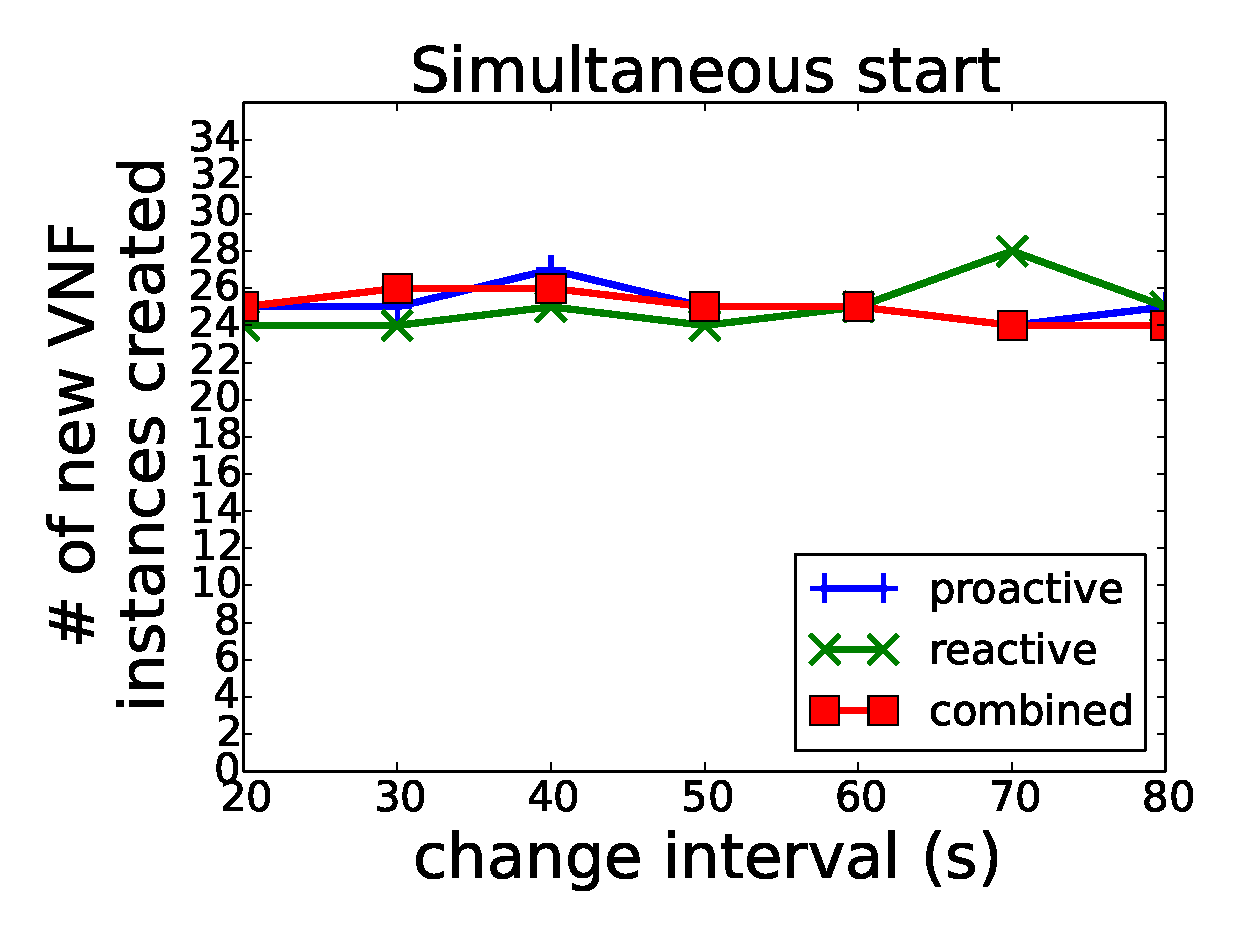
\includegraphics[width=\columnwidth]{chap-scalims/figure/nf-creation1.eps}
  \end{subfigure}
  \begin{subfigure}[t]{0.49\linewidth}
     \centering
     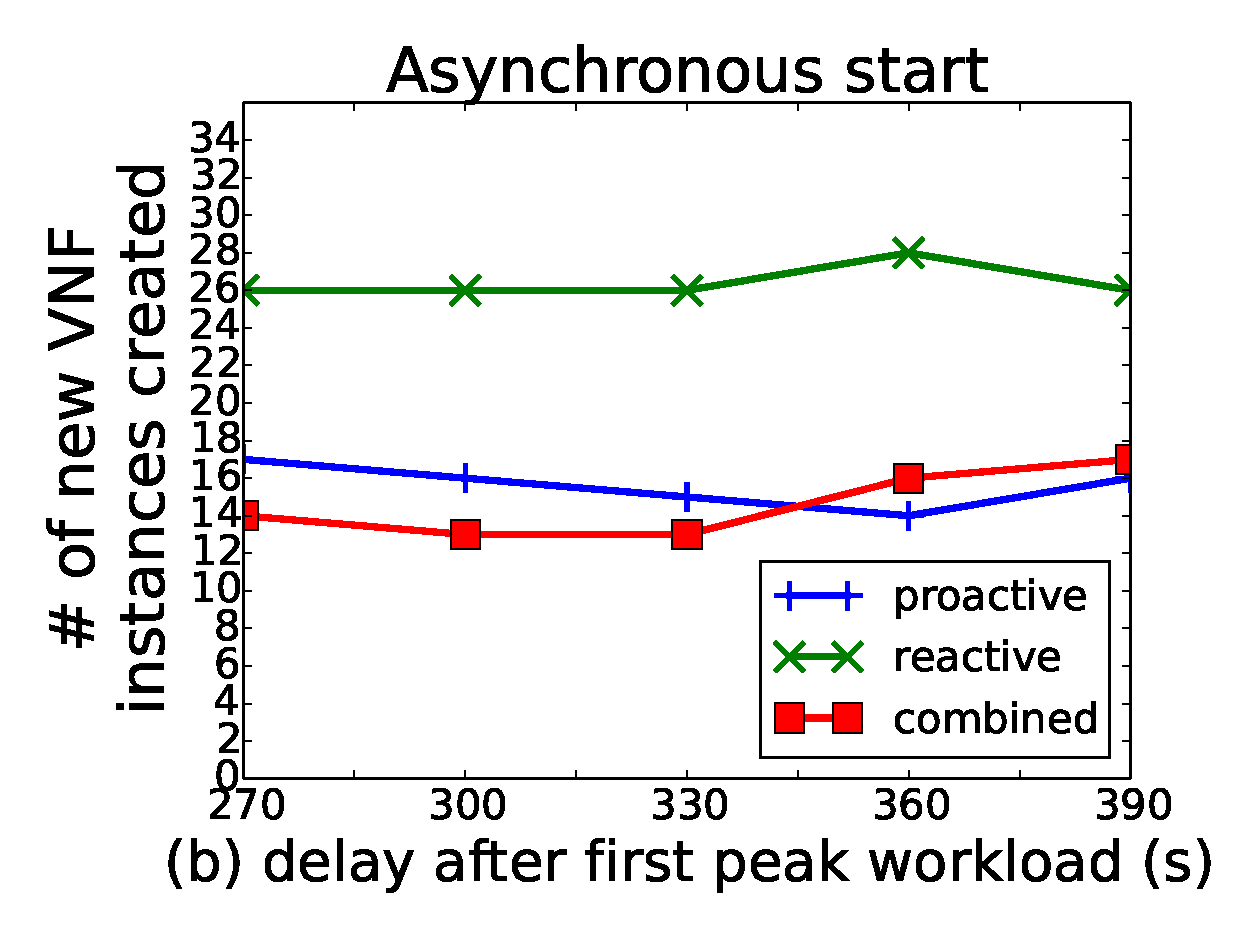
\includegraphics[width=\columnwidth]{chap-scalims/figure/nf-creation2.eps}
    \end{subfigure}
        \caption{Overall number of new VNF instances created: (a) simultaneous start; (b) asynchronous start.}
        \label{fig:nf-creation}
\end{figure}

\subsubsection{Simultaneous Start}

\begin{figure}[!h]
        \centering
        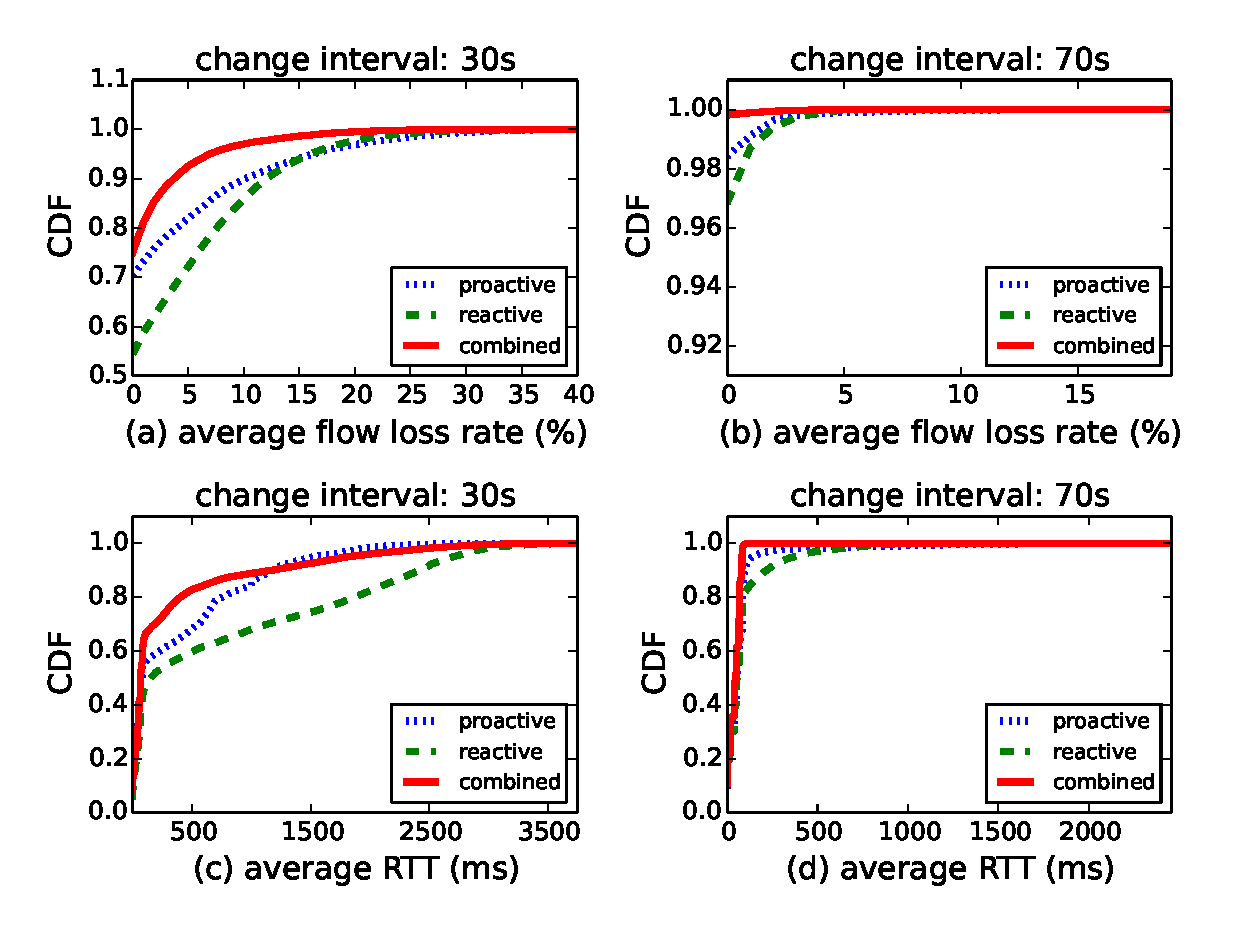
\includegraphics[width=\columnwidth]{chap-scalims/figure/syn-lossrate-rtt.eps}
        \caption{QoS of DP flows: simultaneous start.}
        \label{fig:syn-lossrate-rtt}
\end{figure}

\begin{figure}[!h]
  \begin{subfigure}[t]{0.49\linewidth}
   \centering
   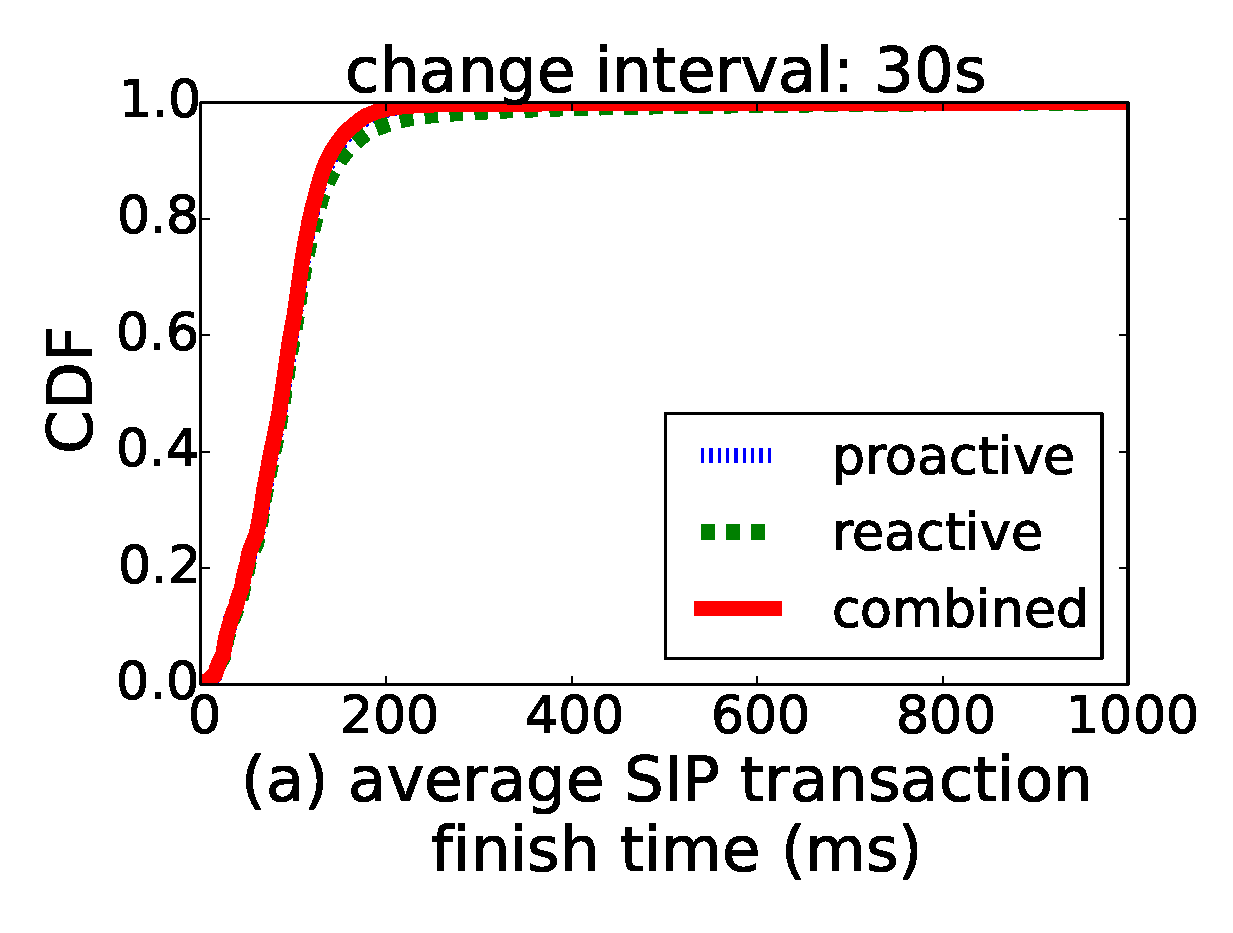
\includegraphics[width=\columnwidth]{chap-scalims/figure/syn-cp1.eps}
  \end{subfigure}
  \begin{subfigure}[t]{0.49\linewidth}
     \centering
     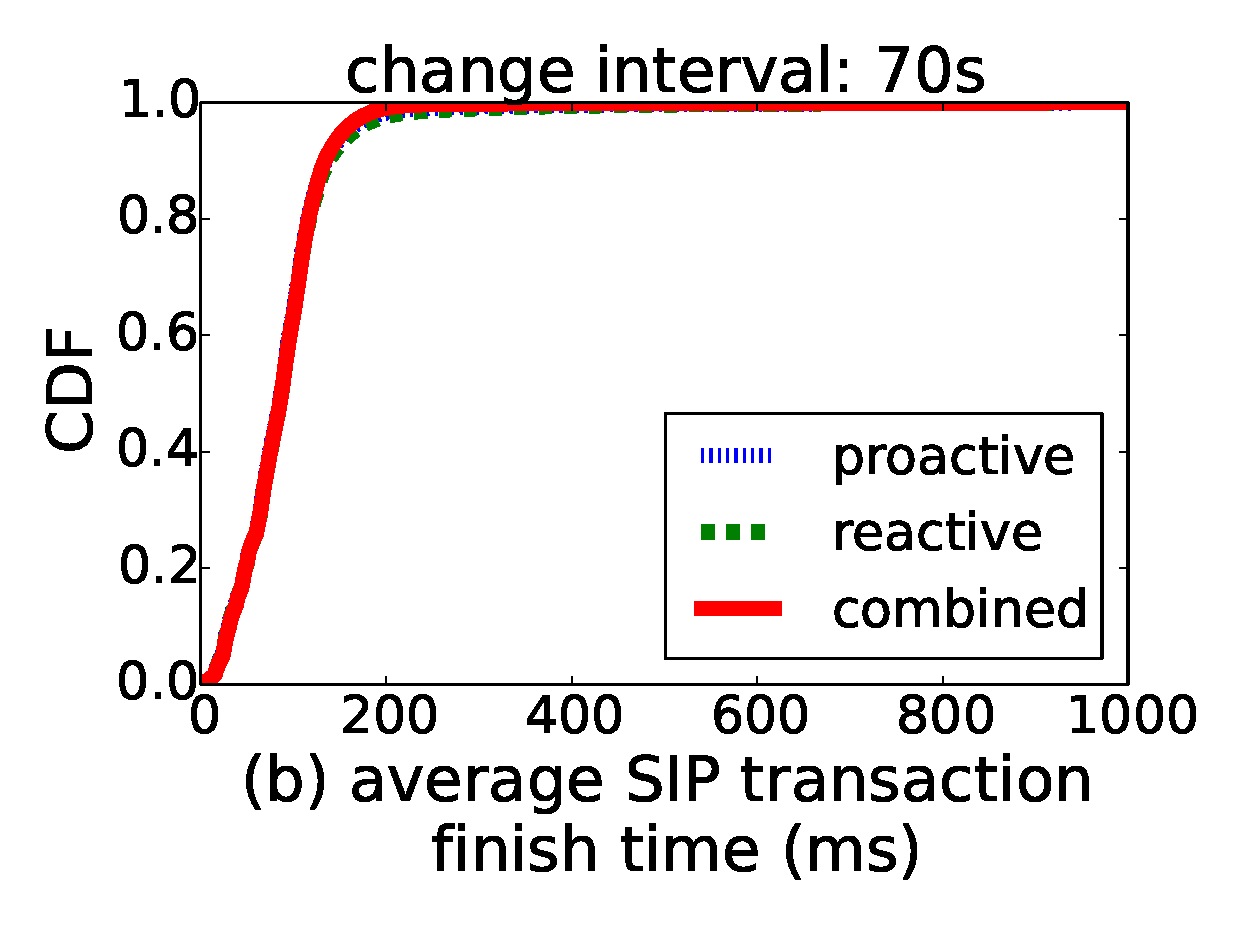
\includegraphics[width=\columnwidth]{chap-scalims/figure/syn-cp2.eps}
    \end{subfigure}
\caption{QoS of CP flows: simultaneous start.}
\label{fig:syn-cp}
\end{figure}

In this set of experiments, each traffic generator starts generating users simultaneously at the rate of $1~users/s$, which gradually increases to $15~users/s$ and then decreases to $6~users/s$. The rate change happens once every \textit{change interval}. The duration of change intervals is set to different values in different experiments.
 %All the traffic generators will start generating users simultaneously at the start of the experiment run,
In this way, the peak workload arrives at each datacenter almost concurrently. %The duration of a change interval is set to 20s, 30s, ... 80s respectively.

%(\chuan{Fig.~\ref{fig:nf-creation}(b): in y labels, instance should be instances'})

Fig.~\ref{fig:nf-creation}(a) shows that the total number of VNF instances provisioned (for both CP and DP service chains) does not differ much under the three schemes. Since the maximum workload on each datacenter arrives at around the same time, the proactive scaling algorithm has no opportunity to decrease the number of provisioned VNF instances by adjusting the service chain path, and therefore the numbers are similar.


Fig.~\ref{fig:syn-lossrate-rtt} plots CDFs of the number of DP flows at different average packet loss rates and average RTTs, and shows that the combined scaling strategy of {\em ScalIMS} out-performs the other two strategies in terms of DP traffic quality. %Due to limited space, we only present the DP traffic quality and CP traffic quality when updated interval is set to 20s and 80s in figure~\ref{fig:syn-lossrate-rtt} and figure~\ref{fig:syn-cp}.
%The reason can be explained as follows.
 Pure reactive scaling adds new instances only when overload occurs. During the boot-up time of new instances, traffic continues to arrive at the overloaded VNF instances, resulting in a high packet loss rate and then high RTT. Pure proactive scaling adjusts VNF instances once every scaling interval. During each scaling interval, increased workload may have overloaded the system. The best performance is achieved combining both proactive and reactive scaling.

Fig.~\ref{fig:syn-cp} shows that the average SIP transaction completion time is similar with the three schemes. This is because scaling of CP service chains is not triggered as often as DP service chains, since each instance of a CP VNF is able to handle a large number of SIP transactions. %Second, the overload threshold for CP VNF is set to a smaller value (70\% of the overload threshold), due to the fact that we observe constant CP VNF crash when CP VNF is on brink of overloading.

%We also Even though we can set a smaller threshold for overload detection to improve the performance of pure reactive scaling approach, but this will inevitably provision more NF instances and decrease resource utilization rate. In order to show this phenomena,

%I didn't managed to produce good result for this set of experiment on IBM cloud, has to delete it.
%To evalaute the impact of the overload threshold in reactive scaling, we conduct another set of experiments by running pure reactive scaling with thresholds set to 80\% of the default overload detection threshold. The results are shown as ``reactive 80\%" in Fig.~\ref{fig:syn-lossrate-rtt} and Fig.~\ref{fig:syn-cp}. We observe that even though decreasing the threshold improves the quality of the user traffic, the quality is still worse than the combined approach.% letting alone the additional created VNF instances during the experiment.

%Figure~\ref{fig:syn-cp} shows CP user traffic quality and performance of the 3 approaches are similar. First, CP scaling is not triggered very often as compared to DP, because CP VNF is able to handle a large amount of SIP transactions. Second, the overload threshold for CP VNF is set to a smaller value (70\% of the overload threshold), due to the fact that we observe constant CP VNF crash when CP VNF is on brink of overloading.

\subsubsection{Asynchronous Start}

\begin{figure}[!h]
  \begin{subfigure}[t]{0.49\linewidth}
   \centering
   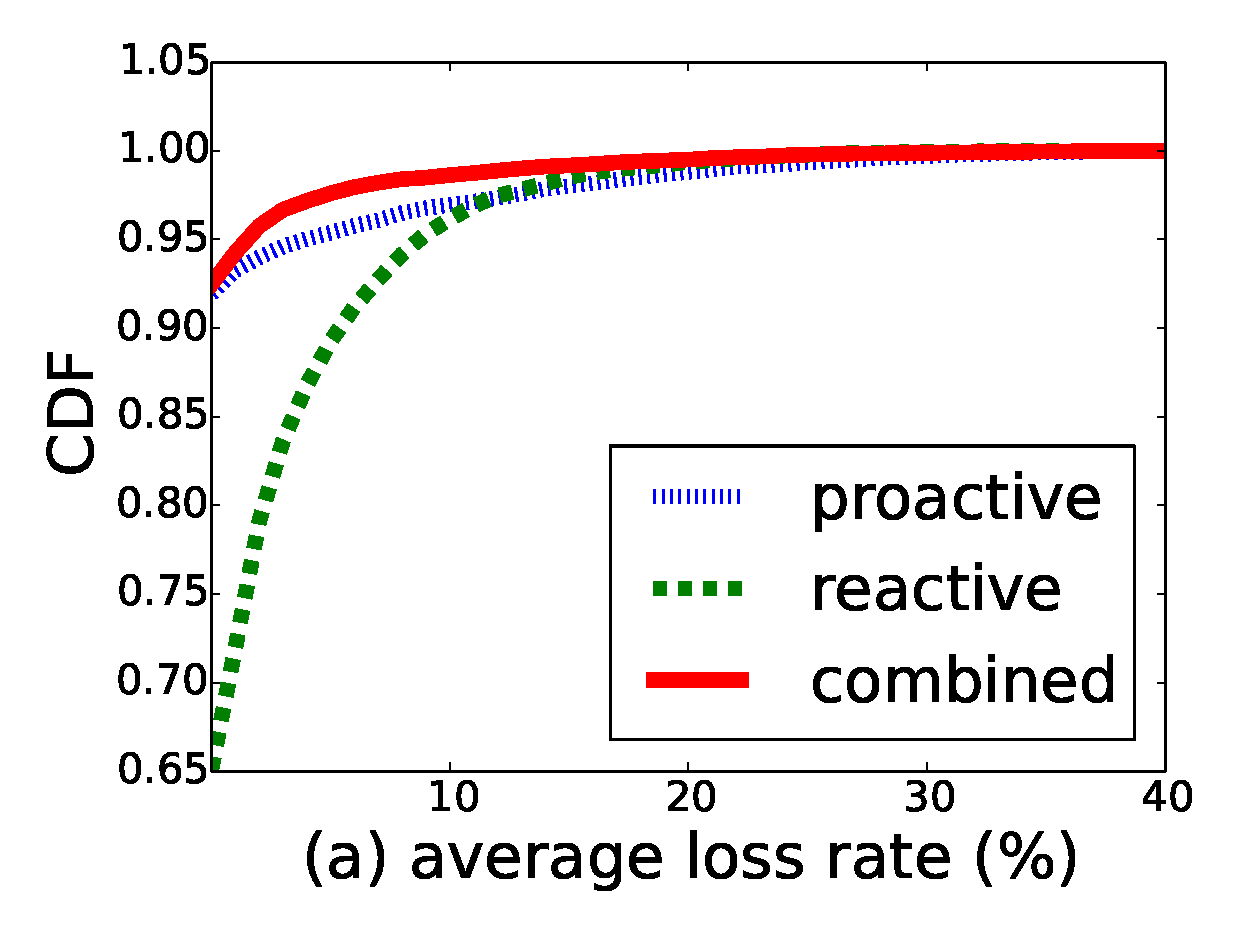
\includegraphics[width=\columnwidth]{chap-scalims/figure/nonsyn-rttloss1.eps}
  \end{subfigure}
  \begin{subfigure}[t]{0.49\linewidth}
     \centering
     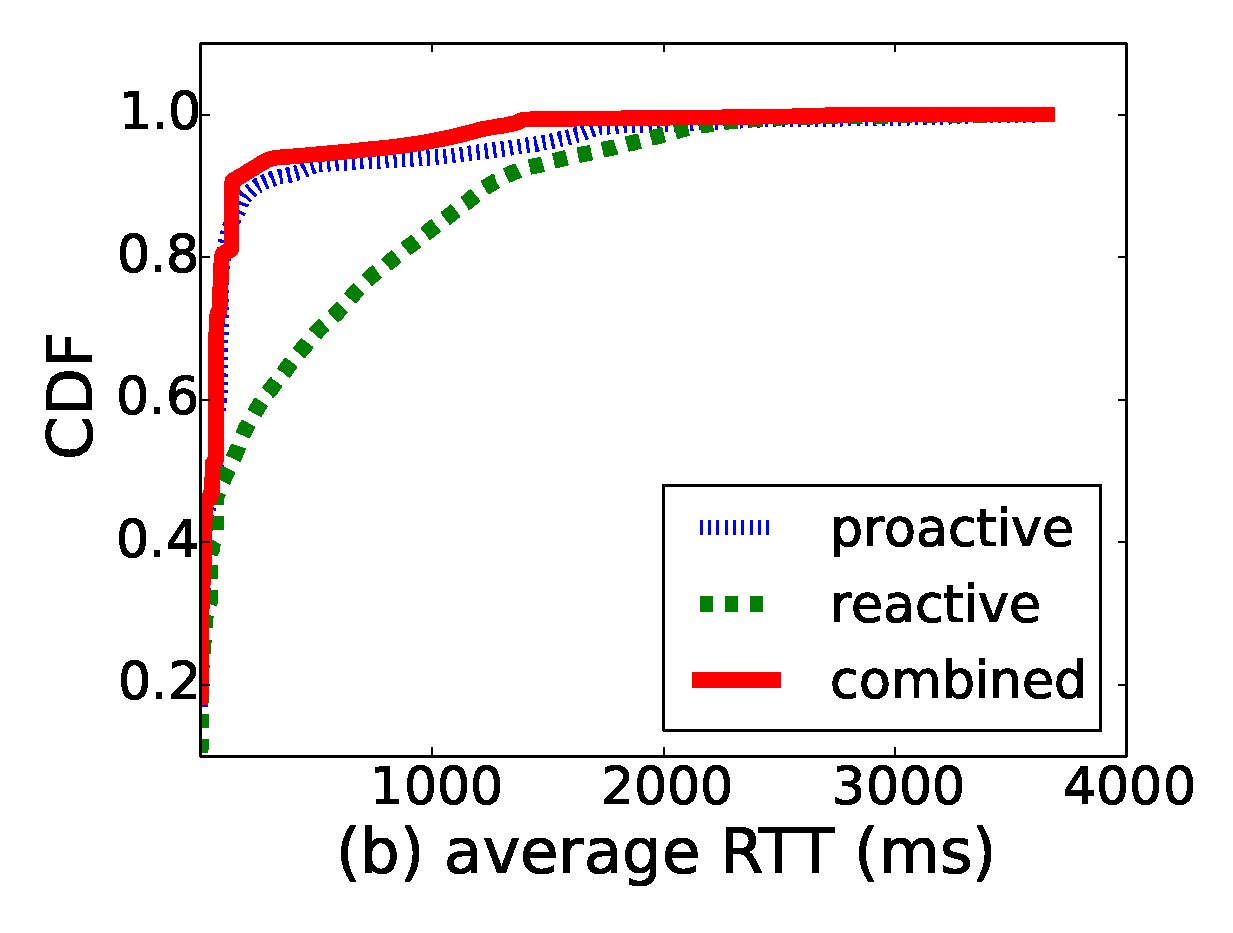
\includegraphics[width=\columnwidth]{chap-scalims/figure/nonsyn-rttloss2.eps}
    \end{subfigure}
\caption{QoS of DP flows: asynchronous start.}
\label{fig:nonsyn-rttloss}
\end{figure}

In this set of experiments, %traffic generators are not started at the same time.
the traffic generator in the Tokyo datacenter is started first, followed by the traffic generators in Hong Kong, in Houston and then in London. %The start time of the traffic generator in a subsequent datacenter is delayed for a configurable period of time after that of the previously started traffic generator.
 In this way, the peak workload in different datacenters does not occur at the same time. Each traffic generator increases its user generation rate from 5 $users/s$ to 15 $users/s$ and then reduces it to $5~users/s$, with a 30s change interval.

In Fig.~\ref{fig:nf-creation}(b), the start delay between traffic generators in Tokyo and in Hong Kong is set according to the values on the x axis, while start delays between traffic generators in Hong Kong and in Houston, and between traffic generators in Houston and in London, are set to 120s. We observe that the number of VNF instances created with the combined scaling approach is similar to proactive scaling approach, but always smaller than reactive scaling approach. Fig.~\ref{fig:nonsyn-rttloss} shows that the traffic quality is the best with the combined approach as well. The performance of CP SIP transaction completion time under asynchronous start is very similar to the results presented in Fig.~\ref{fig:syn-cp}. %Due to limited space, we show the DP traffic quality with 300s delay value in figure~\ref{fig:nonsyn-rttloss}. The combined approach out-performs reactive scaling by a large margin in terms of both flow loss rate and measured RTT.

%We can see that the number of provisioned NF instances in combined scaling approach is apparently smaller than that of purely reactive scaling approach. And even with smaller NF instance provision number, the combined scaling approach has a better data plane traffic quality than the reactive scaling approach.

\subsubsection{Explanation}

\begin{figure}[!h]
        \centering
        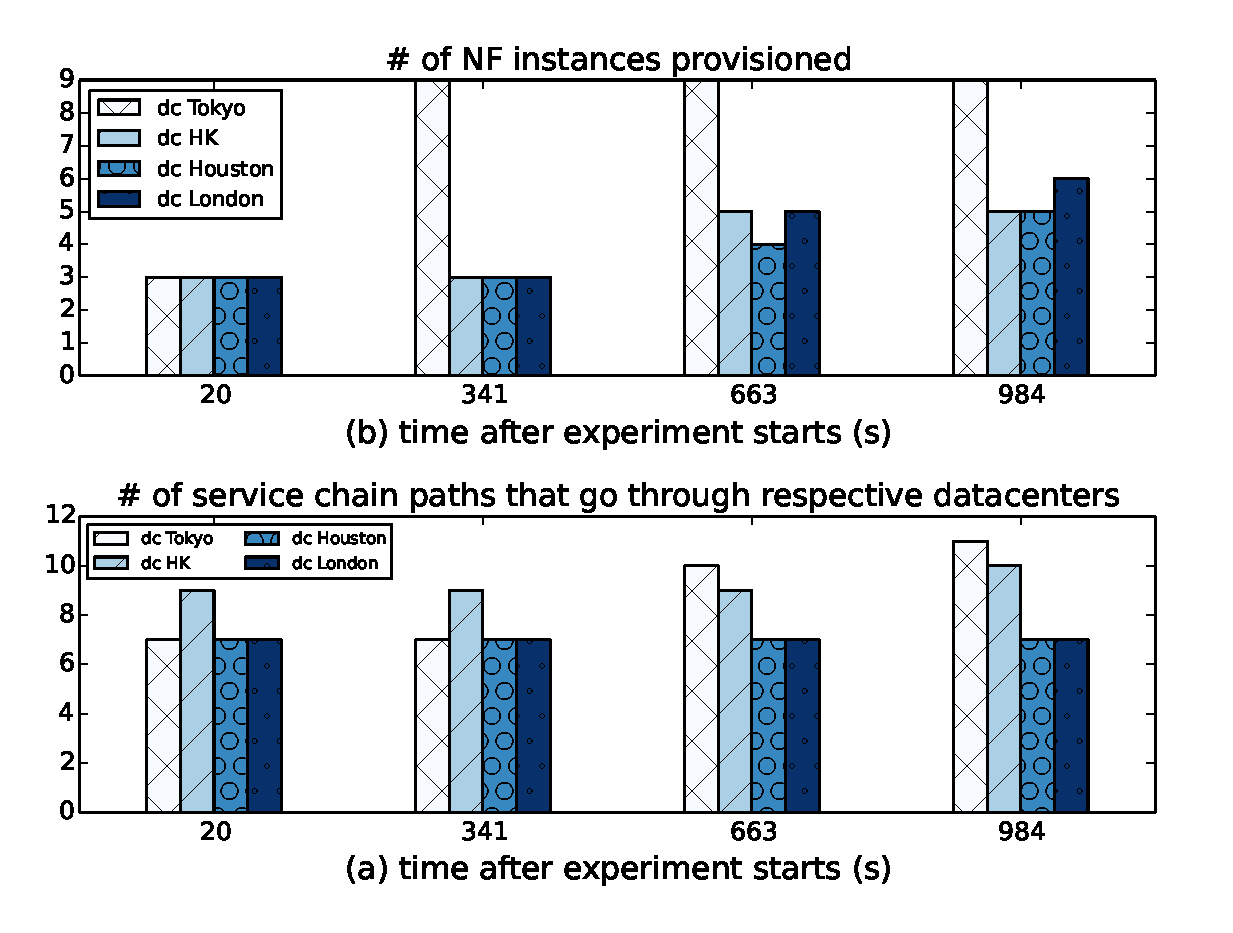
\includegraphics[width=1\columnwidth]{chap-scalims/figure/nonsyn-reason.eps}
        \caption{%Delayed start time is 300s
		%(a) Number of provisioned VNF instances in each datacenter versus time. (b) The number of service chain paths going through different datacenters.
		 Number of VNF instances in/service chain paths through each datacenter: asynchronous start.}
        \label{fig:nonsyn-scpath}
\end{figure}

Why can the combined scaling strategy perform well even when it creates a smaller number of VNF instances? The Tokyo datacenter sees the peak workload first, leading to the provisioning of many VNF instances in the datacenter, which later become redundant and will be buffered for 10 scaling intervals. When peak workload arrives at other datacenters, the global controller can re-use the buffered VNF instances by creating service chain paths traversing the Tokyo datacenter. %, increasing resource utilization efficiency. %We can see from the experiment results that as a side effect, traffic quality also gets improved. %The reason is illustrated in Fig.~\ref{fig:nonsyn-scpath}.
 These phenomena are exhibited in Fig.~\ref{fig:nonsyn-scpath}. %(a) shows the number of VNF instances created in each datacenter verses the time after the experiment starts. We can see that due to the early arrival of peak workload, many VNF instances are provisioned in Tokyo datacenter by 341s. After that time, the number of service chain paths that go through Tokyo datacenter increases from 7 to 11 (Fig.~\ref{fig:nonsyn-scpath}(b)) because the global controller schedules more DP traffic flows to re-use these existing VNF instances. Because these existing VNF instances are buffered and reused, DP traffic flows do not go through overloaded instances, improving the quality experienced by the DP flows.



%\subsection{Evaluation in an Emulation Cluster}

%We also evaluate the performance of \textit{ScalIMS} on our own computing cluster containing 8 IBM blade servers, each equipped with 16 cores, 80GB RAM, 500GB SATA disk, and connected to a Gigabyte Ethernet switch. We emulate a datacenter using a server. The inter-datacenter delay is emulated using Linux TC. By default, the 8 datacenters are separated into 4 groups (i.e. $g_0$ to $g_3$, where $g_i$ contains datacenter $i$ and $i+1$). Datacenters in same group are close to each other with an inter-datacenter delay of 5ms. Datacenters in different groups are farrer away from each other and their delays are set according to the corresponding inter-group delay shown in Table~\ref{table:stat}.

%\vspace{-3mm}
\begin{comment}
\subsection{Evaluation in Emulation Cluster}

%\subsubsection{Links with Large Delays}

We next investigate whether {\em ScalIMS} is able to effectively detect links with high delays and shift the traffic away from these links, using our own 8-server emulation cluster. We emulate a datacenter using one server, and vary inter-datacenter delays with Linux TC \cite{tc}. The 8 emulated datacenters are divided into 4 groups (i.e. $g_0$ to $g_3$, where $g_i$ contains datacenter $i$ and $i+1$). The delay between datacenters in the same group is set to 5ms, and the delay between datacenters in different groups is set according to Table~\ref{table:stat}.

In this set of experiments, traffic generators increase user production rate from 1 $user/s$ to 12 $users/s$ and then decrease the rate to 6 $users/s$, with a 50s change interval. The maximum allowed end-to-end flow delay is 50ms. At 350s after each experiment starts, we deliberately increase the delay between groups $1$ and $3$ to 65ms, and hence the global controller would avoid using links between groups $1$ and $3$.

\begin{figure}[!t]
  \begin{subfigure}[t]{0.49\linewidth}
   \centering
   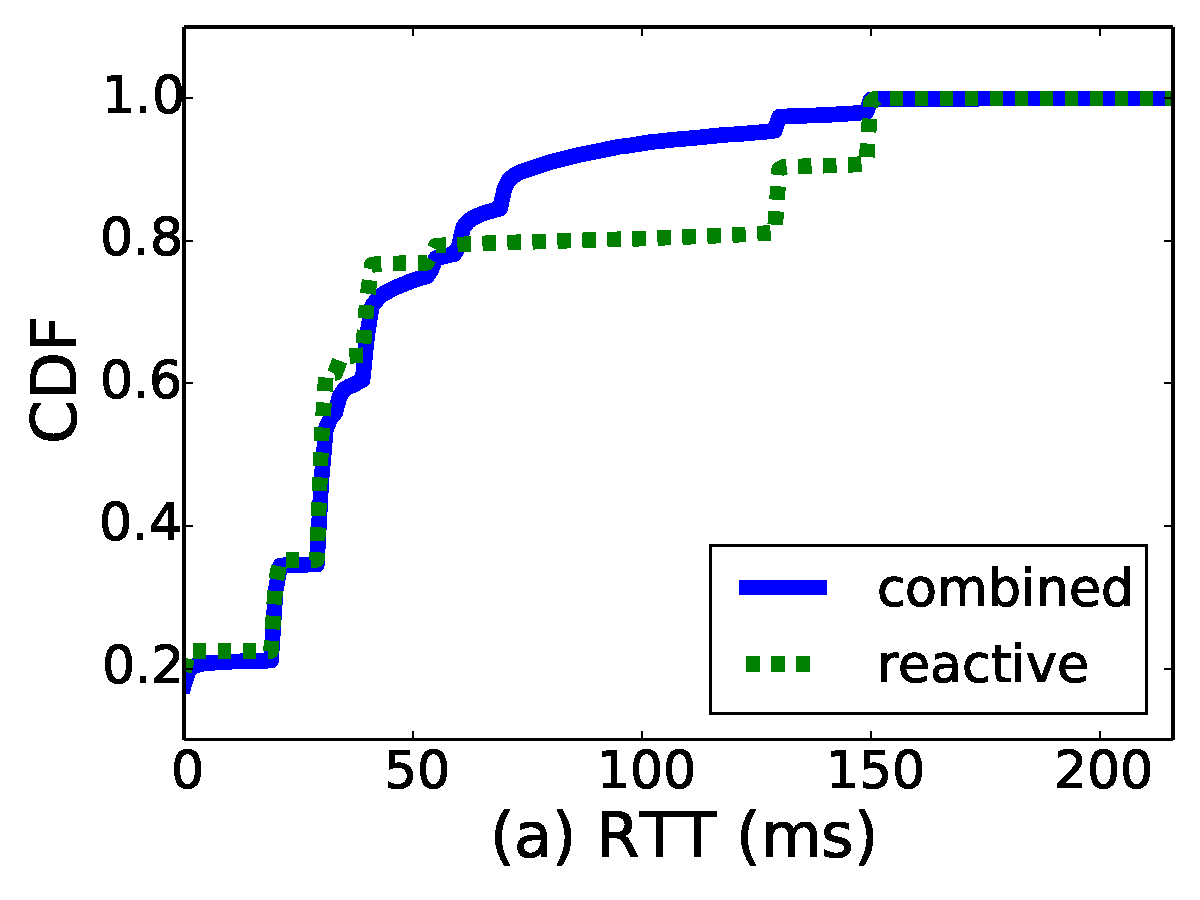
\includegraphics[width=\columnwidth]{chap-scalims/figure/delay1.pdf}
  \end{subfigure}
  \begin{subfigure}[t]{0.49\linewidth}
     \centering
     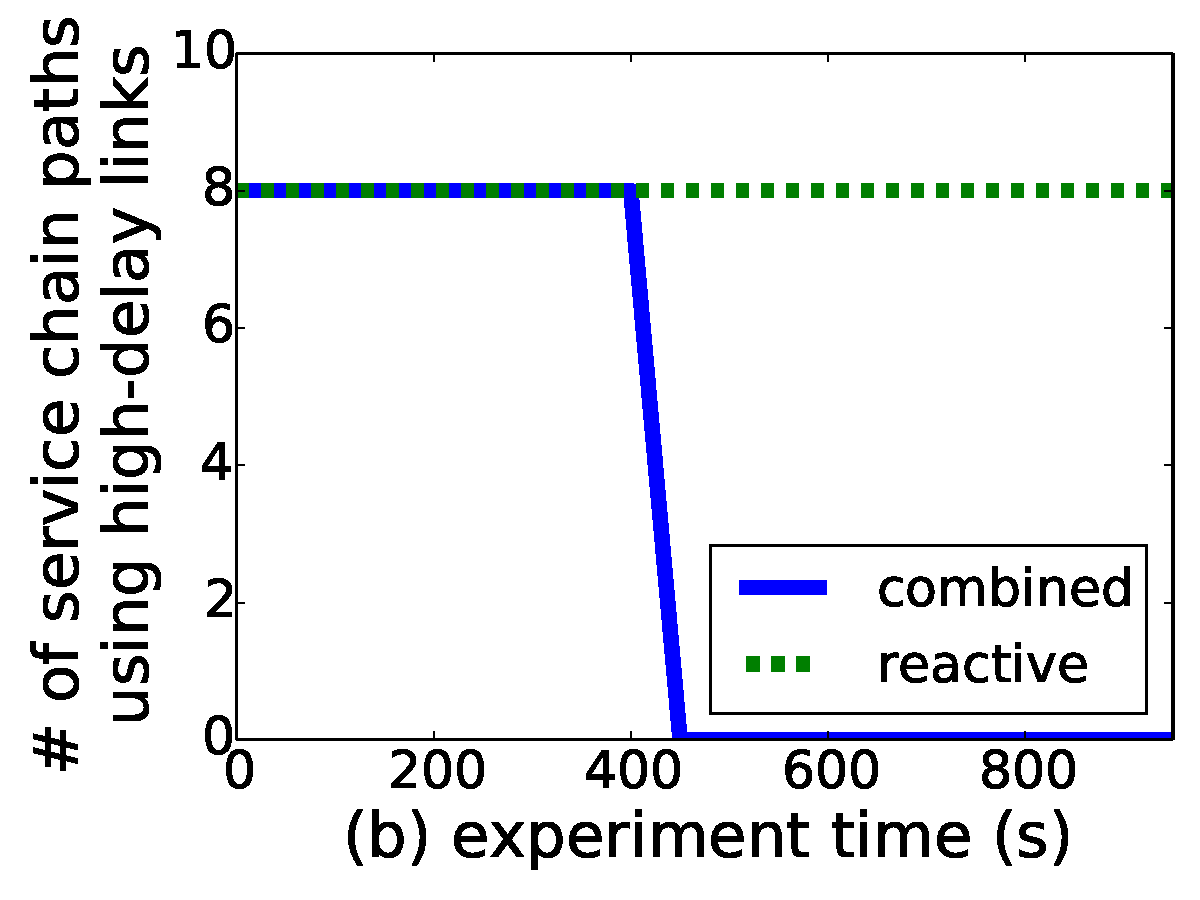
\includegraphics[width=\columnwidth]{chap-scalims/figure/delay2.pdf}
    \end{subfigure}
    \caption{Emulation results in case of links with large delays.}% (a) CDF of flow RTT. (b) Number of service chain paths that use the links between group 1 and group 3.}
    \label{fig:delayrun}
    \vspace{-5mm}
\end{figure}

%\begin{figure}[!t]
%        \centering
%        \includegraphics[width=1\columnwidth]{figure/delay.pdf}
%        \caption{Emulation results in case of links with large delays.}% (a) CDF of flow RTT. (b) Number of service chain paths that use the links between group 1 and group 3.}
%        \label{fig:delayrun}
%\end{figure}

Fig.~\ref{fig:delayrun} (a) shows that with {\em ScalIMS}, the number of flows whose average RTT is smaller than 100ms is 15\% more than that with the reactive scaling approach. Fig.~\ref{fig:delayrun}(b) illustrates that the global controller can effectively re-compute new service chain paths, avoiding the high-delay links. The result of the proactive scaling strategy is similar with the combined scaling strategy because they share the same path computation algorithm.
\end{comment}
% At about 400s, the number of service chain paths that use the high delay links drops from 8 to 0, boosting the quality of the DP media flow.


\begin{comment}
%\subsubsection{Scaling Interval Consistency}

We also evaluate the impact of our design on maintaining scaling interval consistency as discussed in Sec.~\ref{Inconsistency}, by comparing it with one where flows are not tagged with scaling intervals and local controllers always route flows using servcice chain paths in the current scaling interval. In this set of experiments, we generate 15 calls per second between datacenter 0 and 1 for 5 minutes. Enough VNF instances are pre-provisioned on 3 datacenters (datacenters $0-2$) to serve the traffic. The global controller alternates service chain paths from datacenter 0 to datacenter 1 and from datacenter 1 to datacenter 0 from (0, 0, 0, 1, 1) and (1, 1, 1, 0, 0) to (0, 2, 2, 2, 1) and (1, 2, 2, 2, 0) in each scaling interval. %The global controller is placed on datacenter 2, so that there is basically no delay between global controller and datacenter 2 local controller. On the other hand,
The delays between datacenters 0 and 2 and between datacenters 1 and 2 are both set to 400ms.
If a local controller finds out that it is not on a flow's service chain path, it applies a rule that drops all the packets of this flow. %The packet loss rates of all the generated flows are shown in Table~\ref{tab:con}.

%\textbf{First}, we run experiment with our distributed flow routing fully enabled. \textbf{Second}, we run experiment without scaling interval tagging, and force subsequent datacenters on service chain path to always use the service chain path under their current scaling interval.


We find that without scaling interval tagging, 18 out of 8722 flows ($0.2\%$) are completely not received by their receivers. On the contrary, all 8724 flows are received with 0\% loss rate when the scaling interval tagging is enabled. This is because when service chain paths from datacenter 0 to datacenter 1 and from datacenter 1 to datacenter 0 are switched from (0, 2, 2, 2, 1) and (1, 2, 2, 2, 0) to (0, 0, 0, 1, 1) and (1, 1, 1, 0, 0), datacenter 2 enters the next scaling interval earlier. There is a small time window when datacenter 2 starts using service chain path (0, 0, 0, 1, 1) and (1, 1, 1, 0, 0) while datacenter 0 and datacenter 1 are still in the previous scaling interval, using service chain path (0, 2, 2, 2, 1) and (1, 2, 2, 2, 0). Datacenters 0 and 1 continue sending flows to datacenter 2 during that time window, but datacenter 2 finds that it is not on the service chain path of this flow, thus dropping all the packets. We omit the related figures due to space constraint.
\end{comment}

\begin{comment}
\begin{table}[!t]
%\captionsetup{font=footnotesize}
\centering
\caption{Loss rate when scaling interval tagging is enabled/disabled}
\label{tab:con}
\resizebox{.9\columnwidth}{!}{
\begin{tabular}{|l|l|l|}
\hline
\begin{tabular}[c]{@{}l@{}}Loss rate \\ summary\end{tabular}                 & \begin{tabular}[c]{@{}l@{}}With scaling\\ interval tagging\end{tabular} & \begin{tabular}[c]{@{}l@{}}Without scaling\\ interval tagging\end{tabular} \\ \hline
\begin{tabular}[c]{@{}l@{}}\# of generated \\ flows\end{tabular}              & 8724                                                                    & 8722                                                                       \\ \hline
\begin{tabular}[c]{@{}l@{}}\# of flows with\\ 0\% packet loss\end{tabular}   & 8724                                                                    & 8704                                                                       \\ \hline
\begin{tabular}[c]{@{}l@{}}\# of flows with\\ 100\% packet loss\end{tabular} & 0                                                                       & 18                                                                         \\ \hline
\end{tabular}
}
\end{table}
\begin{comment}

\begin{comment}
\begin{table}[h]
\centering
\caption{Flow loss rate when scaling interval tagging is enabled/disabled}
\label{tab:con}
\resizebox{\columnwidth}{!}{
\begin{tabular}{|c|c|c|}
\hline
                                                                                      & \begin{tabular}[c]{@{}c@{}}With scaling\\ interval tagging\end{tabular} & \begin{tabular}[c]{@{}c@{}}Without scaling\\ interval tagging\end{tabular} \\ \hline
\begin{tabular}[c]{@{}c@{}}Number of flows with \\ 0\% packet loss rate\end{tabular}  & 8724                                                                    & 8704                                                                       \\ \hline
\begin{tabular}[c]{@{}c@{}}Number of flows with\\ 100\% packet loss rate\end{tabular} & 0                                                                       & 18                                                                         \\ \hline
\end{tabular}
}
\end{table}
\end{comment}

\section{Summary}\label{sec:scalims-conclusion}

\subsection{Comparison with Existing Work}

%\noindent \textbf{Scalability.}
Scaling of service chains has been investigated in a single server, a computing cluster or a datacenter. CoMB~\cite{sekar2012design} focus on scaling VNFs in a single server, %for better performance. %Even though their implementations achieve good performance, but it lacks generality and flexibility.
 by designing customized architecture to unify VNFs inside a single server. % and they can not be cannot be seemlessly integrated into existing SDN framework.
 %E2~\cite{palkar2015e2}, Stratos~\cite{gember2012stratos} and Slick~\cite{anwer2015programming} study scaling of VNFs in a single SDN-enabled datacenter.
 E2~\cite{palkar2015e2} scales VNF service chains in a single datacenter, %scales VNF instances  within a computing cluster connected through SDN enabled switches through
 exploiting high-performance inter-VNF data paths through SDN-enabled switches. % it has its own high performance inter-VNF datapath.
Stratos~\cite{gember2012stratos} %scales VNF instances by
 jointly consider VNF placement and flow distribution within a datacenter, using on-demand VNF provisioning and VM migration to mitigate hotspots.

%To our knowledge, there do not exist NFV management frameworks that scale VNF service chains across geo-distributed datacenters. % while \textit{ScalIMS} concentrates on scaling NFV service chains across datacenters.
The management systems mentioned above cannot be directly extended to the multi-datacenter setting. One primary reason is that SDN controllers~\cite{mckeown2008openflow} are extensively used in these systems to facilitate routing, scaling and load-balancing within a datacenter. However, SDN controllers are rarely available in the WAN, except for among datacenters of a few large providers such as Google~\cite{jain2013b4} and Microsoft~\cite{hong2013achieving}.
%\chuan{change this reference to B4 or SWAN}. %It is extremely hard for a SDN controller to set up flows on other datacenters, which incurs too much delay and hurts flow performance. One possible approach is to deploy one SDN-enabled management system in each datacenter, but there is no existing work on coordinating the behavior of such independent scaling systems, needed for deploying and scaling geo-distributed service chains. %However, scaling systems on different datacenters need to agree on complicated task such as coordinated VNF instance provision and collective flow routing. And all these problems call for an efficient design of a multi-datacenter scaling system.
%A new management system is in need, that efficiently coordinates service chain deployment and scaling, as well as flow routing, across multiple data centers.
 \textit{ScalIMS} is a NFV management system that efficiently coordinates service chain deployment and scaling, as well as flow routing, across multiple data centers. \textit{ScalIMS} uses similar methodologies as in~\cite{palkar2015e2} and \cite{gember2012stratos} when scaling NFV service chains within a datacenter, but adopts a novel distributed flow routing approach and a proactive scaling strategy to scale NFV service chains across multiple datacenters.

Similar with \textit{ScalIMS}, Klein \cite{qazi2016klein} also scales NFV service chains across multiple datacenters. However, it focuses on scaling EPC system \cite{epc} and does not use a hybrid scaling strategy as \textit{ScalIMS} does. Ren et al. \cite{ren2016dynamic} propose a VNF dynamic auto scaling algorithm for 5G networks, but it lacks a real-world implementation when compared to \textit{ScalIMS}.

\subsection{Conclusion}

This chapter proposes \textit{ScalIMS}, a NFV management system designed to deploy and scale service chains spanning geo-distributed datacenters, using the case of an IMS. \textit{ScalIMS} features joint proactive and reactive scaling of DP and CP service chains, for timely and cost-effective provisioning of practical network services. Evaluation of our prototype implementation on IBM SoftLayer cloud shows that: (i) \textit{ScalIMS} improves QoS of user traffic by a large margin when compared with pure reactive scaling; (ii) when peak workload arrives asynchronously over the geographic span, \textit{ScalIMS} effectively reduces the total number of VNF instances provisioned while guaranteeing excellent QoS. %\textit{Finally}, we show that distributed routing framework of \textit{ScalIMS} accurately route flows across geo-distributed datacenters.

%\vspace{-2mm}


\chapter {\nfactor: A Resilient NFV System using the Distributed Actor Model}
\label{ch:nfvactor}
\lhead{\chaptername \ \ref{ch:nfvactor}.\ \emph{\nfactor}}

This chapter discusses the design and implementation of \nfactor. The chapter starts with an introduction to \nfactor using section \ref{sec:nfvactor-introduction}. Then the motivation for using the actor model is given in section \ref{sec:nfvactor-motivation}. The overall architecture of \nfactor~is given in \ref{sec:nfvactor-runtime-and-controller}, followed by the discussion of the APIs exposed by~\nfactor~for building NFs in section \ref{sec:nfvactor-nf-api}. The protocol for flow replication and migration is illustrated in section \ref{sec:nfvactor-migration-replication}. The performance of \nfactor~is demonstrated in section \ref{sec:nfvactor-evaluation}. Finally, the related work of \nfactor~is given in section \ref{sec:nfvactor-related-work} and a summary of \nfactor~is presented in section \ref{sec:nfvactor-conclusion}.

\section{Introduction}
\label{sec:nfvactor-introduction}

Network function virtualization (NFV) advocates moving
{\em network functions} (NFs) out of dedicated hardware middleboxes and running them as virtualized applications on commodity servers \cite{nfv-white-paper}. To enable effective large-scale deployment of virtual NFs, a number of NFV management systems have been proposed in recent years \cite{palkar2015e2, OpenBox, sekar2012design, anderson2012xomb, gember2012stratos, zhang2016opennetvm}, implementing a broad range of management functionalities. Among these functionalities, resilience guarantee, supported by flow migration and failure recovery mechanisms, is of particular importance in practical NFV systems.

% They implement a broad range of management functionalities and two of %A network service typically consists of a sequence of NFs for flow processing, described by a {\em service chain}, \eg, ``firewall $\rightarrow$ intrusion detection system (IDS) $\rightarrow$ loader balancer''.

{\em Resilience to failures \cite{sherry2015rollback,rajagopalan2013pico} is crucial for stateful NFs.}  Many NFs maintain important per-flow states \cite{EnablingNF}: IDSs such as Bro \cite{bro} store and update protocol-related states for each flow for issuing alerts for potential attacks; firewalls \cite{firewall} parse TCP SYN/ACK/FIN packets and maintain TCP connection related states for each flow; load balancers \cite{lvs} may retain mapping between a flow identifier and the server address, for modifying destination address of packets in the flow. It is critical to ensure correct recovery of flow states in case of NF failures, such that the connections handled by the failed NFs do not have to be reset -- a simple approach strongly rejected by middlebox vendors \cite{sherry2015rollback}.

{\em Efficient flow migration \cite{rajagopalan2013split, gember2015opennf, qazi2017high} is important for long-lived flows in case of dynamic system scaling.} Existing NFV systems \cite{palkar2015e2, gember2012stratos} mostly assume dispatching new flows to newly created NF instances when existing instances are overloaded, or waiting for remaining flows to complete before shutting down a mostly idle instance, which are efficient for short flows. Long flows are common on the Internet:  a web browser uses one TCP connection to exchange many requests and responses with a web server \cite{http-keep-alive}; video-streaming \cite{ffmpeg} and file-downloading \cite{ftp} systems maintain long-lived TCP connections for fetching large volumes of data from CDN servers. When NF instances handling such flows are overloaded or under-loaded, migrating flows to other available NF instances enables timely hotspot resolution or system cost minimization \cite{gember2015opennf}.

Even though failure resilience and efficient flow migration are important for NFV systems, enabling light-weight failure resilience and high-performance flow migration within existing NF software architecture has been a challenging task.

Failure resilience in the existing systems \cite{sherry2015rollback,rajagopalan2013pico} is typically implemented through checkpointing: each NF process is regularly checkpointed, and if it fails, the system replays important log traces collected since the latest checkpoint to recover the failed NF. Compared to the normal packet processing delay of an NF that lies within tens of microseconds, the process of checkpointing is heavyweight and can cause extra delay up to thousands of microseconds \cite{sherry2015rollback, rajagopalan2013pico}.

%Flow migration in existing systems is typically governed by centralized controllers \cite{rajagopalan2013split, gember2015opennf} with limited scalability. When an NFV system is scaled up to handle tens of running NFs \cite{palkar2015e2}, the centralized controller may become overloaded when monitoring concurrent flow migration among multiple pairs of NFs. In addition, such a centralized controller is typically an SDN controller, which installs expensive SDN switching rules to update flow routes during flow migration and compromises the overall migration performance. Finally, even though multiple messages have to be exchanged when executing the flow migration protocol, existing systems \cite{rajagopalan2013split, gember2015opennf} still rely on kernel network stack to deliver these messages, which prolongs the migration completion time due to the inefficiency of the kernel network stack \cite{netmap}.

Flow migration in existing systems \cite{rajagopalan2013split, gember2015opennf} is typically governed by a centralized controller. It fully monitors the migration process of each flow by installing SDN rule to update the route of the flow and exchanging messages with the NFs over inefficient kernel networking stack \cite{netmap}. However, a practical NFV system needs to manage tens of running NFs and handle tens of thousands of concurrent flows. To migrate these flows, the controller needs to sequentially execute the migration process of each flow, install a large number of SDN rules and exchange many migration protocol messages through inefficient communication channel, which may prolong the flow migration completion time and inhibit flow migration from serving as a practical NFV management task.

%Flow migration in existing systems \cite{rajagopalan2013split, gember2015opennf} is typically governed by a centralized controller, which installs SDN switching rule to update flow route during the migration of each flow. Even though multiple messages have to be exchanged when executing the migration protocol, existing systems \cite{rajagopalan2013split, gember2015opennf} still rely on kernel network stack to deliver these messages, which may increase the message passing time due to the inefficiency of the kernel network stack \cite{netmap}. As a practical NFV system usually needs to process tens of thousands of concurrent flows \cite{palkar2015e2}, migrating these flows requires installing and exchanging tens of thousands of SDN rules and migration messages over inefficient kernel networking stack, which may prolong the flow migration completion time and inhibit flow migration from serving as a practical NFV management task.

%    and installing These factors inhibit existing flow migration systems from timely migrating tens of thousands of concurrent flows.

% Besides, enabling flow migration with existing NF software is not trivial: flow migration requires important NF states to be correctly extracted and serialized for transmission. However, a separation between NF states and core processing logic is not enforced in the state-of-the-art NF implementation. OpenNF \cite{gember2015opennf} reports that several thousands lines of patch code must be added to the NF software, \eg, Bro IPS \cite{bro} and Squid caching proxy \cite{squid}, in order to extract and serialize flow states. %

Besides, enabling flow migration with existing NF software is not trivial: OpenNF \cite{gember2015opennf} reports that thousands lines of patch code must be added to existing NF software \cite{bro, squid} in order to extract and serialize flow states, communicate with the controller and control flow migration. This approach mixes the logic for controlling flow migration together with the core NF logic. To maintain and upgrade such an NF, the developer must well understand both the core NF logic and the complicated flow migration process, which adds additional burden on the developer. %and impedes future development of NFV technology.

% Flow migration requires important NF states must be correctly extracted and serialized for transmission. However, a separation between NF states and core processing logic is not enforced in the state-of-the-art NF implementation.  OpenNF \cite{gember2015opennf} reports that several thousands lines of patch code must be added to the NF software (Bro IPS \cite{bro} and Squid caching proxy \cite{squid}) in order to extract and serialize flow states, let alone the source code for controlling flow migration. What's more, as the logic for controlling flow migration is mixed together with core NF logic, it becomes

%This makes the logic that implements flow migration to be mixed together with the core NF logic, making it hard to upgrade and extend both logics.

% Extracting and serializing important NF states have been a

In this chapter, we present \nfactor, a new software framework for building NFV systems with high-performance flow migration and lightweight failure resilience. Unlike previous systems \cite{sherry2015rollback, rajagopalan2013pico, rajagopalan2013split, gember2015opennf} which augment existing NF software with resilience support, \nfactor~explores new research opportunities brought by a holistic approach: \nfactor~provides a general framework with built-in resilience support by exploiting the distributed actor model \cite{actor-wiki}, and exposes several easy-to-use APIs for implementing NFs. Internally, \nfactor~delegates the processing of each individual flow to an unique flow actor. The flow actors run in high-performance runtime systems, handle flow processing and ensure their own resilience in a largely decentralized fashion. \nfactor~brings three major benefits.

$\triangleright$ {\em Transparent resilience guarantee.} \nfactor~ensures that once the NFs are implemented with the provided APIs, failure resilience of the NFs is immediately guaranteed. \nfactor~decouples resilience logic from core NF logic by incorporating resilience operations within the framework and only exposing APIs for building NFs. Using the APIs, programmers are fully liberated from reasoning about details of resilience operations, but only focus on implementing the processing logic of NFs and handling simple interaction for synchronizing shared states of NFs during resilience operations. The exposed APIs also ensure a clean separation between the core processing logic and important NF states, facilitating resilience operations.

$\triangleright$ {\em Lightweight failure resilience.} With the actor abstraction and cleanly separated NF states, \nfactor~is able to replicate each flow independently without checkpointing the entire NF process. Each flow actor can replicate itself by constantly saving its per-flow state to another actor that serves as a replica.
%, which only involves sending single-trip messages.
This lightweight resilience operation guarantees good throughput, short recovery time and a small packet processing delay.

$\triangleright$ {\em High-performance flow migration.} The use of the actor model enables~\nfactor~to adopt a largely decentralized flow migration process: each flow actor can migrate itself by exchanging messages with other flow actors, while a centralized controller only initiates flow migration by instructing a runtime system about the amount of the flow actors that should be migrated. As a result,~\nfactor~is able to concurrently migrate a large number of flows among multiple pairs of runtime systems.~\nfactor~also replaces SDN switch with a lightweight virtual switch for flow redirection, simplifying flow redirection from updating SDN rule into modifying an runtime identifier number. %which eliminates the expensive operation of SDN rule updating.
The increased parallelism and simplified flow redirection jointly enhance the performance of flow migration.

Our major technical challenge is to build an actor runtime system to satisfy the stringent performance requirement of NFV application. Even the fastest actor runtime systems \cite{chs-rapc-16} may fail to deliver satisfactory packet processing performance due to their actor scheduling strategies and the use of kernel networking stack. To address this challenge, we carefully craft a high-performance actor runtime system by combining the performance benefits of (i) a module graph scheduler to effectively schedule multiple flow actors, (ii) a DPDK-based \cite{dpdk} fast packet I/O framework \cite{bess} to accelerate network packet processing and (iii) an efficient user-space message passing channel which completely bypasses the kernel network stack and improves the performance of both failure resilience and flow migration.

We implement \nfactor~and build several useful NFs using the exposed APIs. Our testbed experiments show that \nfactor~achieves 10Gbps line-rate processing for 64-byte packets, concurrent migration of 600K flows using around 700 milliseconds, and recovery of a single runtime within 70 milliseconds in case of failure. Compared with OpenNF \cite{gember2015opennf}, flow migration completion time in~\nfactor~can be 144 times faster. Compare with FTMB \cite{sherry2015rollback} for replication performance,~\nfactor~achieves similar packet processing throughput and recovery time, but with packet processing latency stabilized at around 20 microseconds. %The source code of \nfactor~is available at \cite{projectcode}.

%Going beyond resilience, a couple of interesting applications can also be efficiently enabled on \nfactor, including live NF update and correct MPTCP subflow processing. They require individual NFs to initiate flow migration, which is hard to achieve in the existing systems. The decentralized and fast flow migration in~\nfactor~enables these applications with ease.

\section{Motivations for Using the Actor Model}
\label{sec:nfvactor-motivation}

Systems that enable failure resilience \cite{sherry2015rollback,rajagopalan2013pico} and flow migration \cite{rajagopalan2013split, gember2015opennf} typically achieve a low level of parallelism: a centralized controller governs the migration of all the flows among multiple NF instances, while an entire NF process has to be checkpointed for replication. If we can improve the parallelism by providing an efficient per-flow execution environment, then each flow can migrate and replicate itself without full-process checkpointing and centralized migration control, leading to improved resilience performance. Such a per-flow execution environment can be modelled by actors.

The actor programming model \cite{actor-wiki, erlang, akka, caf} has a long history of being used to construct massive, distributed systems \cite{actor-wiki, akka, newell2016optimizing, AnalysisActor}. Each actor is a lightweight and independent execution unit. In the simplest form, an actor contains a global unique address, a message queue (mailbox) for accepting incoming messages, several message handlers and an internal actor state (\eg, statistic counter, number of outgoing requests). An actor can send messages to other actors by referring to their addresses, process incoming messages using message handlers, update its internal state, and create new actors. Multiple actors run asynchronously as if they were running in their own threads, simplifying programmability of distributed protocols and eliminating potential race conditions that may cause system crash. Actors typically run on a powerful runtime system \cite{caf}, which can schedule millions of lightweight actors simultaneously.

The actor model is a natural fit to provide a per-flow execution environment for resilient NFV system. We can create one actor as the basic execution environment for a flow and equip the actor with necessary message handlers for service chain processing, flow state replication and migration. Then each actor can process network packets and handle its own resilience by creating new actors and exchanging messages with other actors.

There are several popular actor frameworks \cite{akka, erlang, Orleans, caf}, but none of these frameworks are optimized for building NFV systems. In our initial implementation, we built \nfactor~on top of libcaf \cite{caf}, one of the fastest actor system \cite{chs-rapc-16}. But the overall performance turned out to be less than satisfactory, due to its actor scheduling strategy and the use of kernel networking stack. This inspires us to customize a high-performance actor runtime system (Sec.~\ref{sec:nfvactor-implementation}) for \nfactor.

%\section{Runtime Architecture}

\section {The NFVactor Framework}
\label{sec:nfvactor-runtime-and-controller}

\begin{figure}[!t]
  \centering
  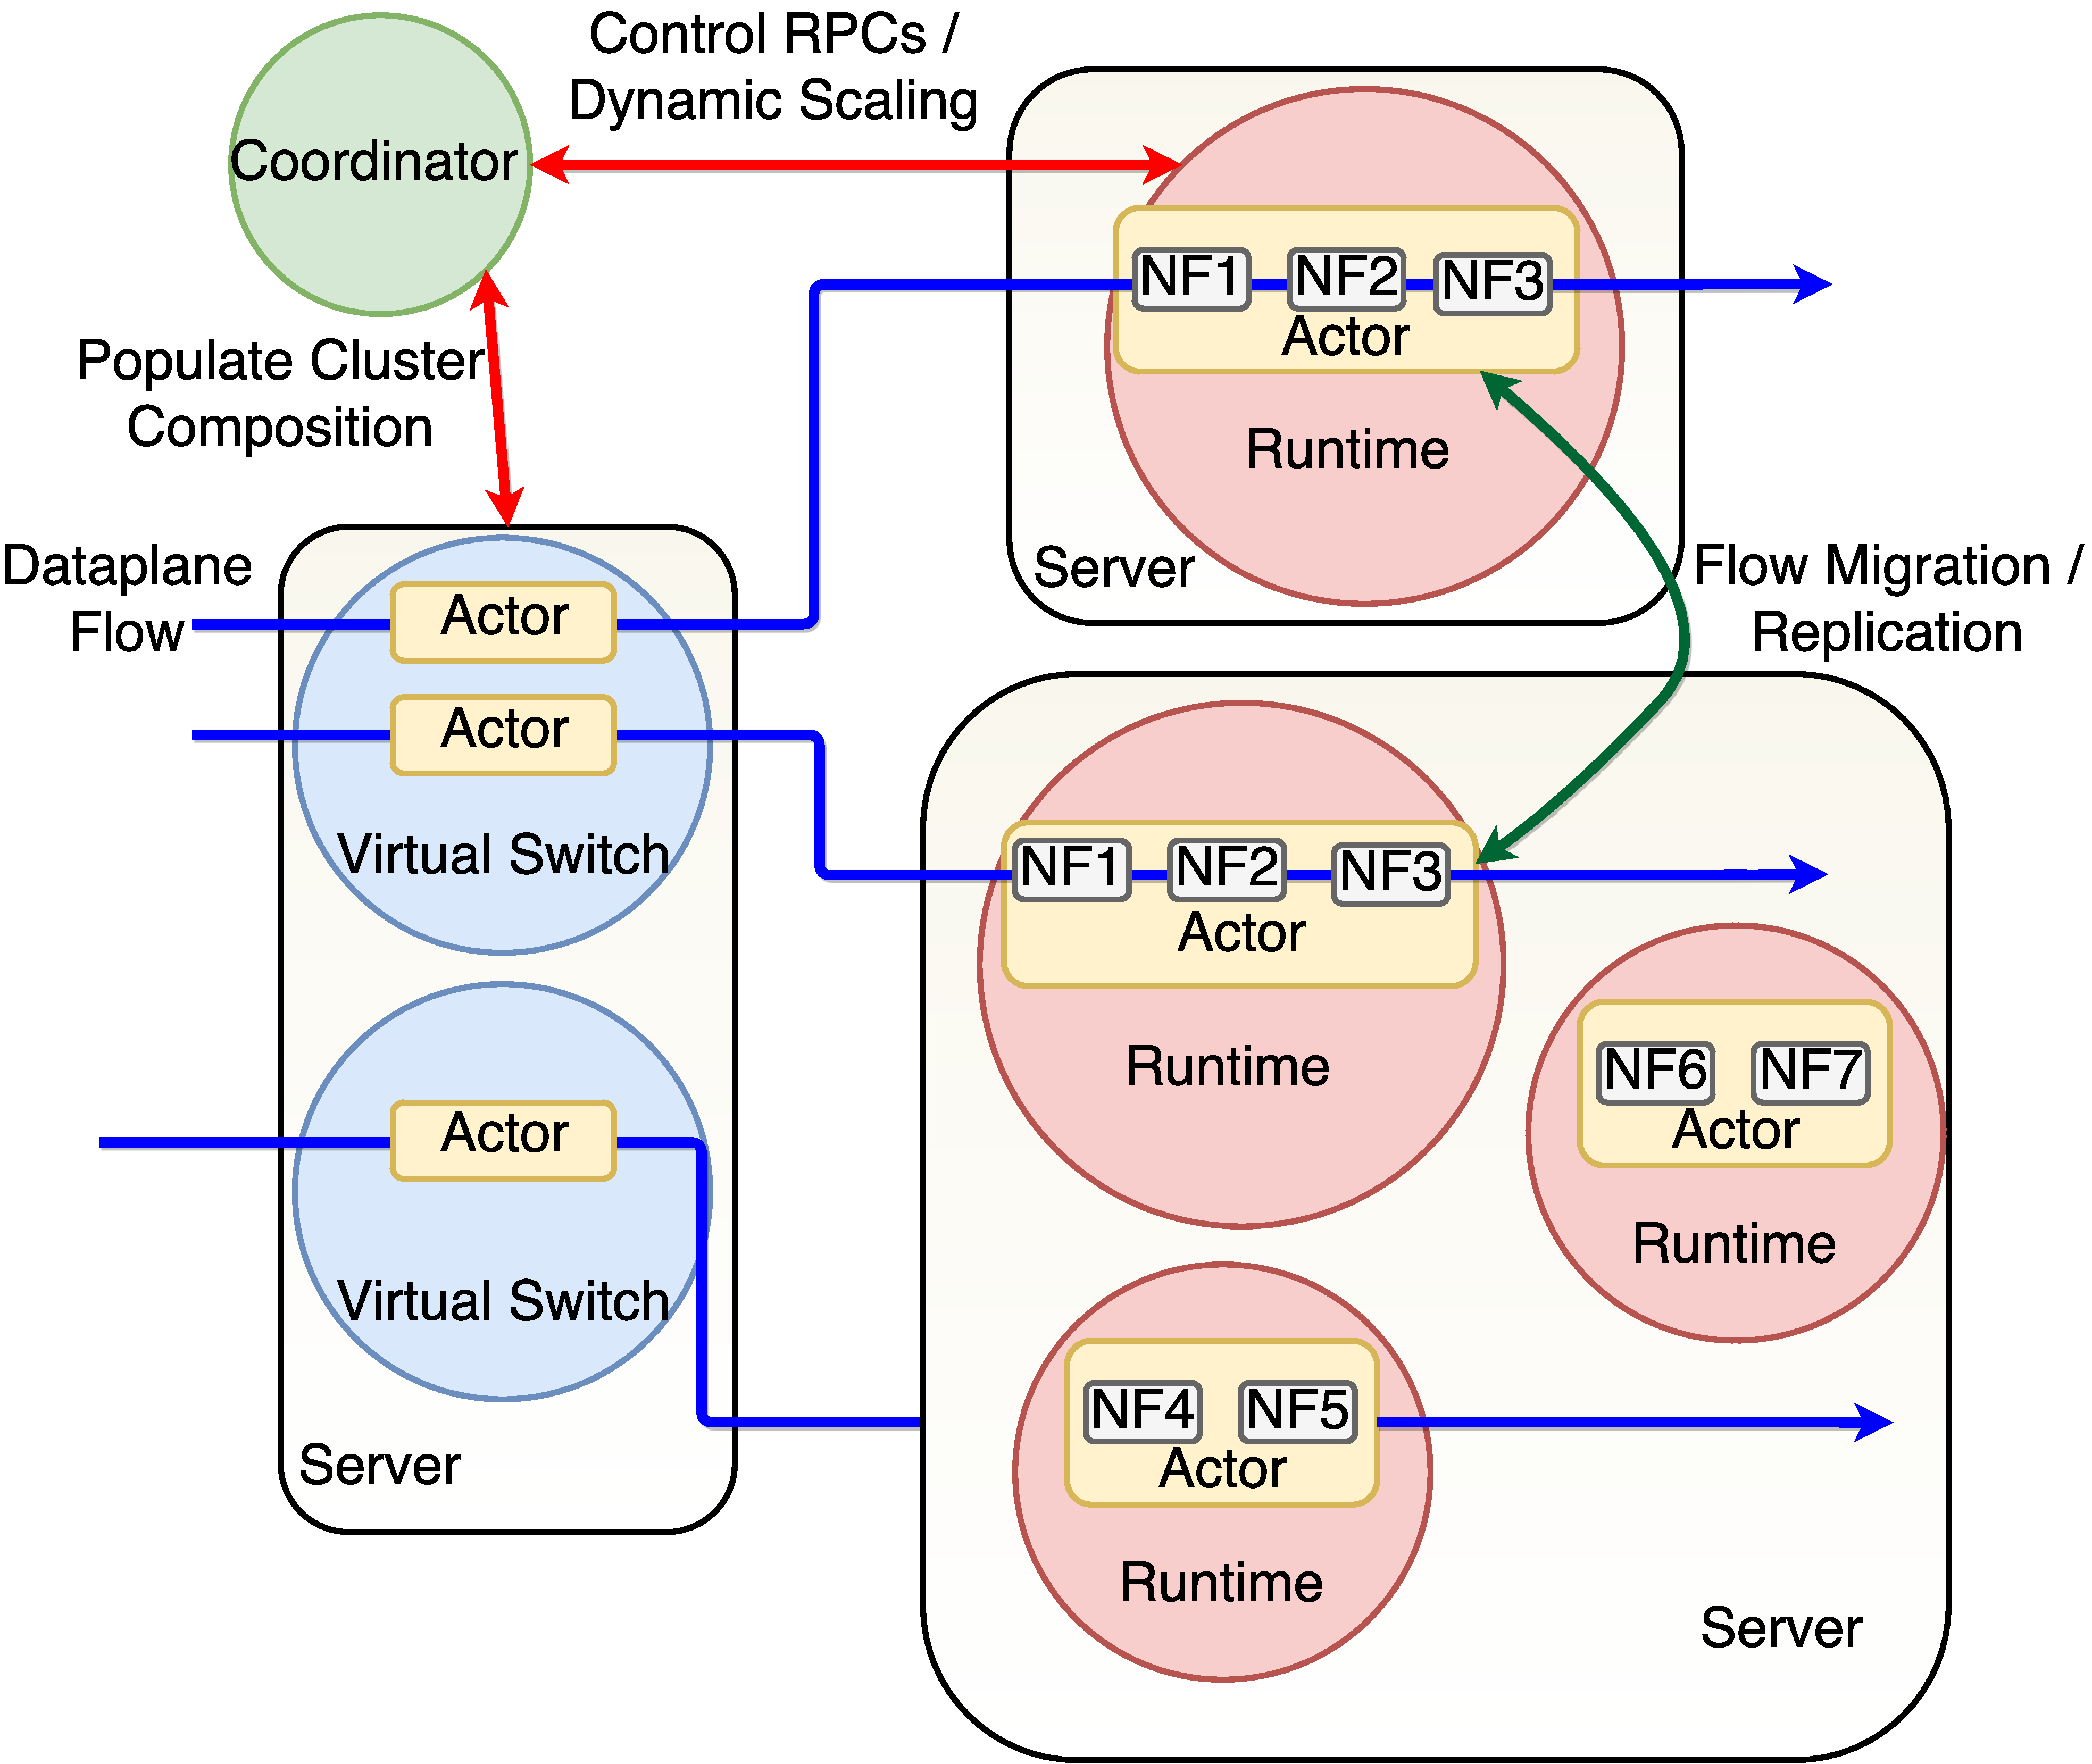
\includegraphics[width=\columnwidth]{chap-nfvactor/figure/new-nfactor-cluster.pdf}
  \caption{An overview of the basic components of \nfactor. Three clusters are shown in this figure: a cluster for provisioning service chain `NF1$\rightarrow$NF2$\rightarrow$NF3', a cluster for service chain `NF4$\rightarrow$NF5' and a cluster for service chain `NF6$\rightarrow$NF7'}
  \label{fig:runtime}
\end{figure}

\subsection{Overview}
\label{sec:overview}

At the highest level, \nfactor~has a layered structure as shown in Fig.~\ref{fig:runtime}. There are three key elements in~\nfactor: (i) runtime systems (referred to as \textit{runtime} for short) that enable flow processing using actors; (ii) virtual switches for distributing flows to runtime systems and sending flows to final destinations; and (iii) a lightweight coordinator for basic system management.

A runtime (Sec.~\ref{sec:runtime}) is the execution environment of flow actors, running on a Docker container \cite{docker} for quick launching and rebooting, and is assigned a globally unique ID upon creation. A virtual switch is a special runtime (Sec.~\ref{sec:virtualswitch}) and serves as the gateway to runtimes.
%Inside a physical server, runtimes and virtual switches are connected with a virtual L2 switch (L2Forward module of BESS \cite{bess}). Different physical servers are inter-connected through a physical Ethernet switch. In~\nfactor,
Runtimes and virtual switches are partitioned into several virtual clusters. In a cluster, the runtimes are initialized with the same service chain (Sec.~\ref{sec:rtsc}) and the virtual switches dispatch flows to the runtimes within the same cluster. The partitioning of virtual clusters enables~\nfactor~to simultaneously provision multiple service chains.

Each virtual switch is configured with an entry IP address. The coordinator sets up proper switching rules %SDN flow rules
to direct dataplane flows to virtual switches, which further dispatch them to runtimes within the same cluster. A runtime creates a dedicated flow actor to process each flow and forward flow packet to its final destination.
%After processing, the outgoing flow packets are sent to another virtual switch in the cluster, which forwards the flow to its final destination.
%\footnote{When our flow replication mechanism is in place, a flow will be sent by replica runtime to the virtual switch, to be forwarded outside (Sec.~\ref{sec:resilience}).}
The coordinator also manages dynamic scaling and failure recovery of~\nfactor~by interacting with runtimes and virtual switches through a series of control RPCs (Sec.~\ref{sec:coordinator}).

Dataplane flows can be migrated and replicated from one runtime to another runtime within the same cluster in a distributed fashion without persistent involvement of the coordinator. To replicate a flow (Sec.~\ref{sec:replicating-runtime}), the corresponding flow actor first launches a replica actor running on another runtime. Then the flow actor constantly saves its private state to the replica actor. The coordinator monitors the flow actor by regularly checking the liveness of the flow actor's runtime. In case of the runtime failure, the replica actor substitutes the flow actor and resumes normal flow processing. To migrate a flow (Sec.~\ref{sec:migration}), the flow actor initializes a target flow actor on another runtime. Then the flow actor contacts the virtual switch to redirect the flow to the target actor, followed by transmitting its private state to the target target. When the migration finishes, the original flow actor destroys itself and the target flow actor continues to process the flow.

\subsection{Runtime}
\label{sec:runtime}

\nfactor~employs a carefully designed, uniform runtime system to run flow actors. Within a runtime, we adopt a {\em one-actor-one-flow} design principle: a dedicated flow actor is created to handle each flow received by the runtime. Packet processing by NFs and resilience operations are all implemented as reactive message handlers of the flow actor. The runtime timely schedules each flow actor to react to the various events, so that each flow actor can process flow packets and manage its own resilience in a largely decentralized fashion. Our one-actor-one-flow principle improves the parallelism of resilience operations while the overhead for creating and managing per-flow actors is significantly reduced (Sec.~\ref{sec:micro-benchmark}) due to our efficient runtime design. This principle serves as the basis for high-performance resilience support.

%To further demonstrate how a runtime works, we first show the internal structure of a runtime, followed by its overall work flow to process data-plane flows and remote actor messages. Finally, we discuss the service chain model adopted by each runtime.

\subsubsection{Internal Structure}

\begin{figure}
		\centering
		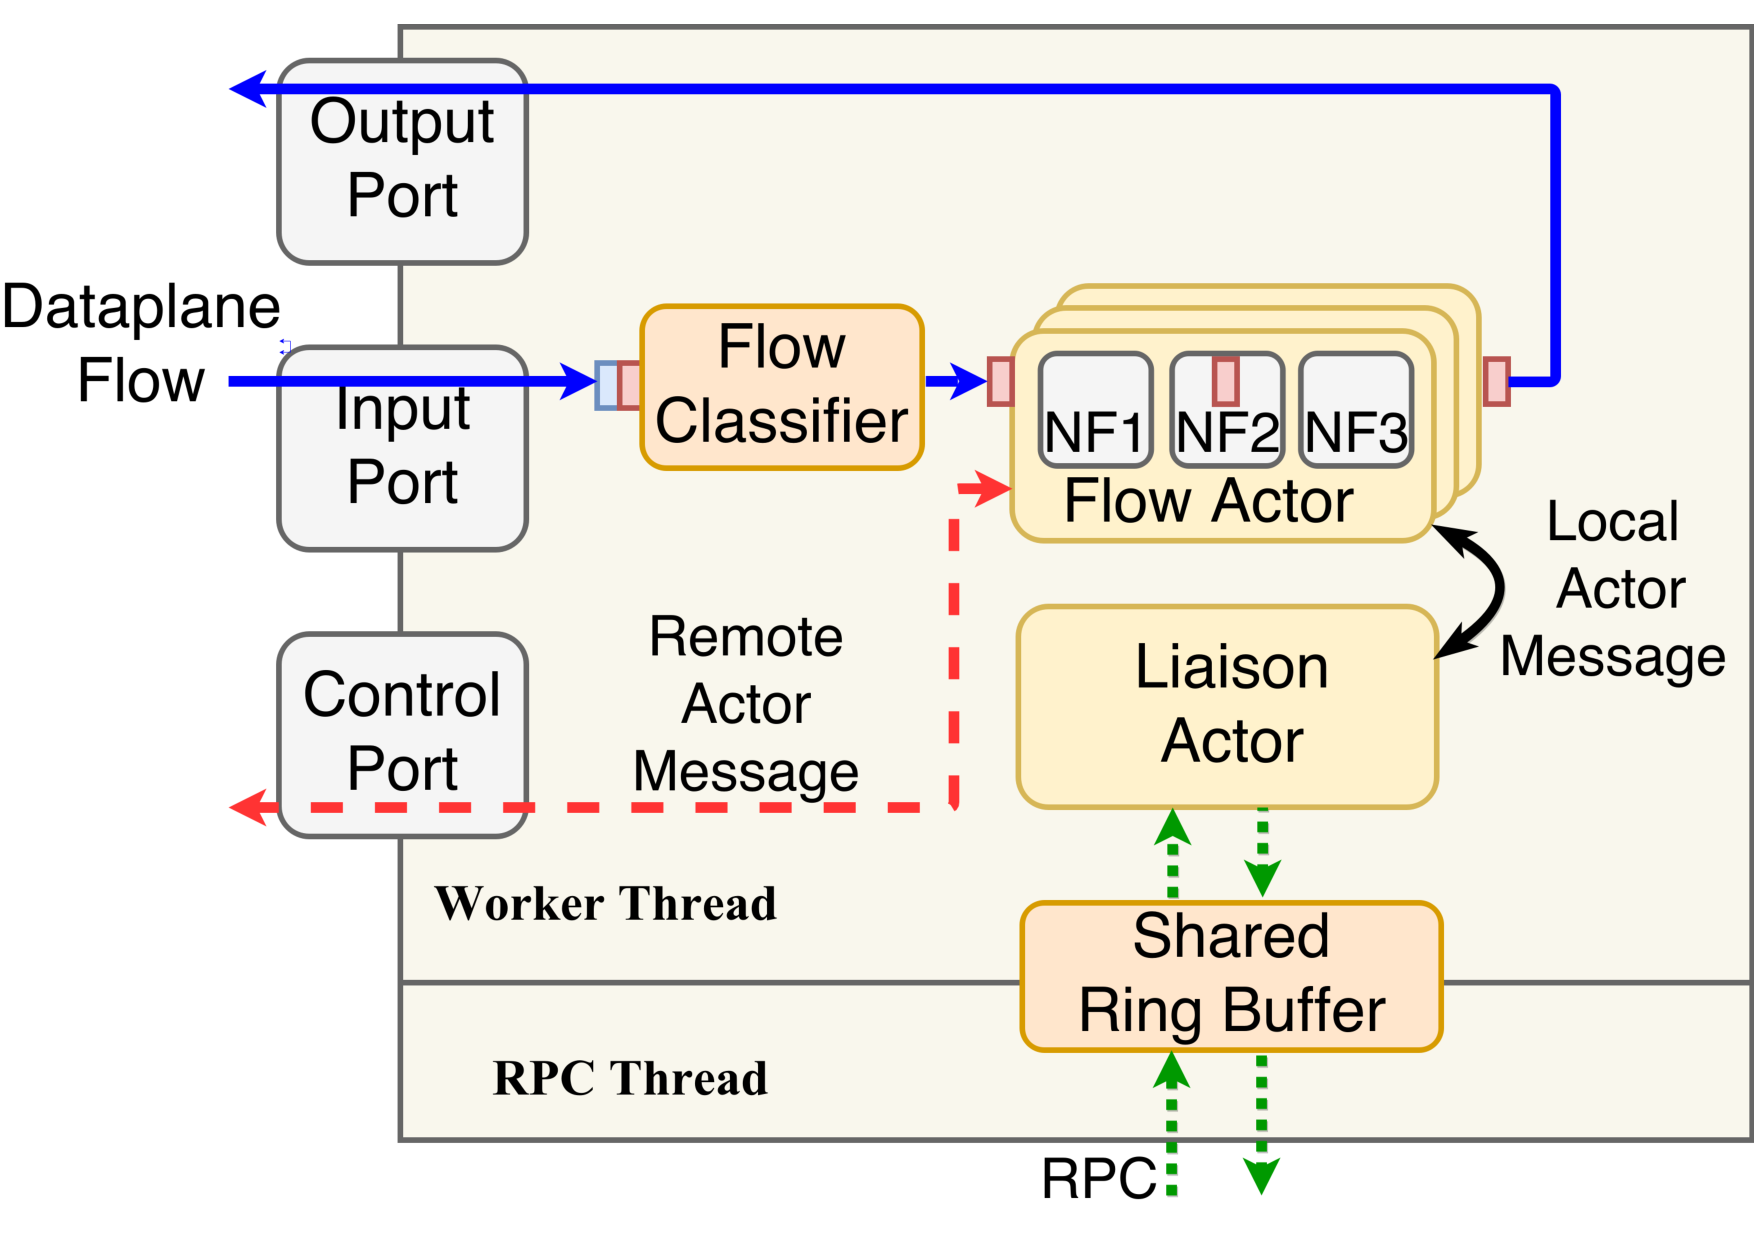
\includegraphics[width=\columnwidth]{chap-nfvactor/figure/new-nfactor-runtime-arch.pdf}
		\caption{The internal structure of a runtime.}
\label{fig:runtime-arch}
\end{figure}

Fig.~\ref{fig:runtime-arch} shows the internal structure of a runtime. Each runtime is configured with one worker thread and one RPC thread. The worker thread actively polls the three ports shown in Fig.~\ref{fig:runtime-arch} and is pinned to a dedicated CPU core to minimize the performance impact caused by thread scheduling. The RPC thread responds to RPC requests sent from the coordinator, for basic system management operations (Sec.~\ref{sec:coordinator}). The three ports are high-speed virtual NICs (ZeroCopyVPort in BESS \cite{bess}) and they are connected to a virtual L2 switch (L2Forward module of BESS) inside a physical server. The worker thread can bypass the kernel and directly fetch network packets from these ports.

\subsubsection{Work Flow}

The runtime has three basic work flows:

\noindent \textbf{Process Dataplane Flows:} The worker thread constantly polls dataplane flow packets from the input port. For each packet, the worker thread uses the 5-tuple of the packet (\ie, source IP address, destination IP address, transport-layer protocol, source port and destination port) to retrieve the corresponding flow actor and sends the packet to the flow actor for processing. Running in its own logical thread, the flow actor processes the packet along the configured service chain and then sends the processed packet out from the output port.

\noindent \textbf{Process Remote Actor Messages:} During distributed flow migration and replication, {\em remote actor messages} are exchanged among actors running on different runtimes. The runtime is equipped with a reliable message passing channel (Sec.~\ref{sec:nfvactor-implementation}) to reliably send and receive remote actor messages over the control port. The received remote actor messages are handed over to the destination actors for processing. The sent remote actor messages are reliably delivered to their receivers.

\noindent \textbf{Process Control RPCs:} The RPC thread forwards received RPC requests to a {\em liaison actor} in the worker thread through the shared ring buffer. The liaison actor coordinates with flow actors via {\em local actor messages}, to handle RPC requests sent from the coordinator.

%\textbf{Customized Actor Library:} To effectively run all these tasks while scheduling actors to react to events, we design a customized actor library (Sec.~\ref{sec:implementation}) for the runtime, equipped with a module graph scheduler and an user-space message passing channel. In Sec.~\ref{sec:micro-benchmark}, we show that our runtime significantly out-performs existing actor runtimes when scheduling actors to process network packets.

\subsubsection{Service Chain}
\label{sec:rtsc}

Each runtime is configured with a sequential service chain (\eg, firewall$\rightarrow$NAT$\rightarrow$load-balancer) and initializes all the NFs along the service chain upon booting. When the flow actor processes packets, it calls the $process\_pkt(input\_pkt, fs, ss)$ API (Sec.~\ref{sec:nfvactor-nf-api}) of each NF according to the service chain structure to implement the service chain processing logic.

%Due to the flexibility of the actor model, we believe that advanced service graph models \cite{OpenBox} can be easily embedded into~\nfactor~as well.

\subsection{Virtual Switch}
\label{sec:virtualswitch}

A virtual switch is a special runtime where the actors do not run service chains but only a flow forwarding function. An actor in a virtual switch is referred to as a {\em virtual switch actor}. The virtual switch serves as a load-balancing gateway when forwarding flows and a lightweight flow redirector when executing resilience operations.

For flow forwarding, a virtual switch learns runtimes that it can dispatch flows to through RPC requests sent from the coordinator. When a new flow arrives, a virtual switch actor selects a runtime with the smallest workload as the destination and saves its ID. For each flow packet, the virtual switch actor replaces the destination MAC address with the MAC address of the input port of the destination runtime and forwards the packet. %one of the runtimes to forward its flow according to the workload %in a round-robin fashion. A simple round-robin approach is adopted because it runs fast and~\nfactor~is able to effectively resolve hot-spots by flow migration. For subsequent flow packets, the virtual switch actor modifies their MAC address and forwards them to the selected runtime.

During flow migration and replication, each virtual switch actor can independently update the flow route by simply modifying the ID of the destination runtime. Compared with installing flow rules on an SDN switch \cite{rajagopalan2013split, gember2015opennf}, the route update process is lightweight and improves flow migration performance for~\nfactor.

\subsection{Coordinator}
\label{sec:coordinator}

\begin{table}[!h]
\centering
\caption{Control RPCs Exposed at Each Runtime}
\label{table:rpc}
\resizebox{\columnwidth}{!}{
\begin{tabular}{l|l}
\textbf{Control RPC}                                                                                   & \textbf{Functionality}                                                                                                                                              \\ \hline
poll\_workload()                                                                                   & \begin{tabular}[c]{@{}l@{}}Poll the load information \\ from a runtime.\end{tabular}                                                                 \\ \hline
notify\_cluster\_cfg(cfg)                                                                         & \begin{tabular}[c]{@{}l@{}}Notify a runtime/virtual switch  \\the current cluster composition.\end{tabular}                                                             \\ \hline
\begin{tabular}[c]{@{}l@{}}set\_migration\_target(runtime\_id, \\ migration\_number)\end{tabular} & \begin{tabular}[c]{@{}l@{}}Initiate flow migration. It tells \\ the runtime to migrate \\ migration\_num of flows to the \\ runtime with runtime\_id.\end{tabular} \\ \hline
set\_replicas(runtime\_id\_list)                                                                       & \begin{tabular}[c]{@{}l@{}}Set the runtimes with IDs  \\in runtime\_id\_list as the replica.\end{tabular}                                                                \\ \hline
recover(runtime\_id)                                                                          & \begin{tabular}[c]{@{}l@{}}Recover all the flows replicated \\ from runtime with runtime\_id.\end{tabular}                                                 \\ \hline
\end{tabular}
}
\end{table}


The coordinator in \nfactor~is responsible for basic cluster management routines, \eg, monitoring system workload, updating cluster composition,  dynamically scaling runtimes for deployed clusters, and recovering failed runtime in a cluster. As compared to centralized controllers in the existing NFV systems \cite{gember2015opennf, rajagopalan2013split}, the coordinator only uses light-weight RPC calls to initiate the flow migration and replication process.

The coordinator communicates with runtimes via a number of control RPCs summarized in Tbl.~\ref{table:rpc}. It uses $poll\_workload()$ to acquire the current workload on a runtime. It updates cluster composition (including MAC addresses of input/output/control ports, workload status and IDs of all runtimes and virtual switches in the cluster) to all the runtimes and virtual switches in a cluster using $notify\_cluster\_cfg(cfg)$.

To deploy a cluster, the system operator first specifies the composition of a service chain to the coordinator. The coordinator then creates a new cluster with one runtime and one virtual switch, configures the runtime with the specified service chain and installs proper switching rules to forward matching input flows to the virtual switch. The cluster is then dynamically scaled and recovered under the control of the coordinator.

The last three RPCs shown in Tbl.~\ref{table:rpc} are used to initiate flow migration and replication. After issuing these three calls, migration and replication are automatically executed among runtimes without further involving the coordinator.

%\subsection{Dynamic Scaling}
%\label{sec:scaling}

\textbf{Dynamic Scaling.} The coordinator performs dynamic scaling of the runtimes and virtual switches by exploiting the distributed flow migration mechanism. It fully exploits distributed flow migration mechanism to resolve hot spot and shut down mostly idle runtimes.

The coordinator periodically polls the workload statistics from all the runtimes, containing the number of dropped packets on the input port, the current packet processing throughput and the number of active flows. In the current~\nfactor~prototype, the runtime is identified as overloaded if the number of dropped packets exceeds a fixed threshold (100 as in our experiments). This is an effective overload indicator for~\nfactor: an overloaded runtime can not timely poll all the packets from its input port, therefore increasing the number of dropped packets significantly, while the CPU usage is rendered ineffective as the worker thread is a busy-polling thread and uses 100\% of the CPU all the time.

If there is an overloaded runtime in a cluster, the coordinator launches a new runtime in the same cluster and keeps migrating a configurable number of flows from overloaded runtime (500 as in our experiments) to the new runtime, until half of the workload on the overloaded runtime is migrated away. %all the hotspots are resolved. % If the new runtime becomes overloaded, more runtimes are added.
%We add new runtimes instead of moving flows across existing runtimes, since the load on existing runtimes is largely balanced, due to the load-balancing functionality of virtual switches.
If runtimes in a cluster become largely idle, the coordinator carries out scale-in: it selects a runtime with the smallest throughput, migrates all its flows to the other runtimes, and shuts the runtime down when all the flows have been successfully moved out.

%The coordinator periodically polls the load statistics from all the runtimes, containing the number of dropped packets on the input port, the current packet processing throughput and the number of active flows. Since the worker thread of the runtime is a busy-polling thread and uses 100\% of CPU all the time, CPU usage is not a good indicator to tell whether a runtime has been overloaded. In the current~\nfactor~prototype, the coordinator uses the total number of dropped packets on the input port of a runtime to determine overload, which is a very effective indicator in~\nfactor: an overloaded runtime can not timely poll all the packets from its input port, therefore increasing the number of dropped packets significantly. When the number of dropped packets per second exceeds 100, the runtime is identified as overloaded. If there is at least one overloaded runtime in a cluster, the coordinator launches a new runtime, configures it to run the same service chain, and keeps migrating a configurable number of flows from overloaded runtimes (500 as in our experiments) to the new runtime, until all the hotspots are resolved. If the new runtime becomes overloaded, more new runtimes are added. We add new runtimes instead of moving flows across existing runtimes, since the load on existing runtimes is largely balanced, due to the load-balancing functionality of virtual switches.

\section{NF APIs}
\label{sec:NFAPIs}

\begin{table}[!t]
%	\small
\centering
\caption{APIs for implementing NFs in \nfactor}
\label{table:api}
\resizebox{0.8\columnwidth}{!}{
\begin{tabular}{l|l}
\textbf{API} & \textbf{Usage} \\ \hline
nf.allocate\_shared\_state() & \begin{tabular}[c]{@{}l@{}}Allocate a singleton object\\ containing the shared states.\end{tabular} \\ \hline
nf.allocate\_new\_fs() & \begin{tabular}[c]{@{}l@{}}Create and initialize a new \\ flow state object. %for a new\\ flow actor
\end{tabular} \\ \hline
nf.deallocate\_fs(fs) & \begin{tabular}[c]{@{}l@{}}Deallocate the flow state object\\ upon expiration of the flow actor.\end{tabular} \\ \hline
$\star$~nf.process\_pkt(input\_pkt, fs, ss) & \begin{tabular}[c]{@{}l@{}}Process the input packet using \\ the current flow states of the flow\\ and the shared states of the NF.\end{tabular} \\ \hline
nf.flow\_expires(fs, ss) & \begin{tabular}[c]{@{}l@{}}Update the shared states according\\ to final flow states upon \\ expiration of the flow actor.\end{tabular} \\ \hline
\begin{tabular}[c]{@{}l@{}}nf. flow\_migrate\_out(fs, ss)\\ nf. flow\_migrate\_in(fs, ss)\\ nf. flow\_recover(fs, ss)\end{tabular} & \begin{tabular}[c]{@{}l@{}}Update the shared states using\\ the flow states during flow\\ migration and replication.\end{tabular} \\ \hline
\end{tabular}
}
\end{table}

To create an NF with full resilience support, the programmer should properly implement the APIs listed in Tbl.~\ref{table:api}. We follow two principles when designing these APIs.

{\em First}, StatelessNF \cite{201545} and Split/Merge \cite{rajagopalan2013split} demonstrate that it is possible to build practical NFs by processing each individual flow with its per-flow state and shared state. Inspired by this principle,~\nfactor~employs a core API $process\_pkt(input\_pkt, fs, ss)$ to accomplish the core NF processing logic. It is called by each flow actor when processing the input packet, taking per-flow state and shared state as additional arguments. Several supporting APIs are also provided to manage important NF states. This design %enables us to create several practical NFs for~\nfactor. It also
 ensures a clean separation between useful NF states and the core processing logic of an NF, so that the flow actor always has direct and efficient access to the latest flow states to ease flow migration and replication.

{\em Second}, to properly handle shared state, we treat shared state accessing by an NF as allocating resource from a shared resource pool. For instance, when a NAT processes a flow, accessing shared state usually means allocating an address from a shared address pool. Therefore, when the flow expires, the resource that the flow acquired should be properly released back to the shared resource pool. With the NAT example, this means that the allocated address should be put back into the address pool when the flow expires. However, when the flow is migrated or recovered on another NF instance, without proper synchronization, the resource obtained by the flow may not be correctly released back to the shared resource pool. To resolve this issue in~\nfactor, the programmer should properly store the allocated resource in the per-flow state. They also need to implement the last four APIs shown in Tbl.~\ref{table:api} for properly releasing the acquired resource so that the shared state is correctly synchronized. Our runtime guarantees that the three APIs are timely invoked during flow migration and replication (Sec.~\ref{sec:management}).

%{\em Third}, cluster contains different runtimes, different runtimes should collectively handle the same task. The implementor should guarantee a correct partition of the shared states across different runtimes

%In the rest of this section, we first discuss how each runtime uses the exposed APIs. Then we discuss the implementation details of four example NFs that we build for~\nfactor. Finally, we discuss the limitation of our current API design.

\subsection{How Runtime Uses the APIs}

When a runtime is created, the shared state of each NF along the configured service chain is initialized by calling $allocate\_shared\_state()$ and stored by a storage actor. After a flow actor is created to process a new flow, it first calls $allocate\_new\_fs()$ to create a flow state for each NF and stores these flow states throughout its lifetime. The flow actor processes a packet along the service chain by sequentially calling $process\_pkt(input\_pkt, fs, ss)$ for each NF, passing in the per-flow state, and shared state obtained from the storage actor. The shared state is sent back to the storage actor when the flow actor finishes processing the packet. When the flow actor expires (this is triggered by a per-actor timer), the flow actor first calls $flow\_expires(fs, ss)$ for each NF to update the shared state and then executes some clean-up procedures, including calling $deallocate\_fs(fs)$ to free the flow state. When a flow is migrated or recovered, the flow actor calls the last three APIs shown in Tbl.~\ref{table:api} to synchronize the flow state with the shared state for each NF, followed by executing some clean-up procedures.

\subsection {Example NFs}

\begin{comment}
\begin{algorithm}[!t]
\SetKwProg{Proc}{Procedure}{}{}
\Proc{load\_balancer.process\_pkt(input\_pkt, fs, ss)}{
  \If{fs.server = NULL}{
    {fs.server $\leftarrow$ get\_idlest\_server(ss.server\_list)}\;
    {increase\_workload\_counter(ss.workload\_list, fs.server)}\;
  }
  {send\_packet\_to\_server(input\_pkt, fs.server)}\;
}

\Proc{load\_balancer.flow\_expires(fs, ss)}{
  \If{fs.server $\neq$ NULL}{
    {decrease\_workload\_counter(ss.workload\_list, fs.server)}\;
  }
}

\Proc{load\_balancer.flow\_migrate\_out(fs, ss)}{
  \If{fs.server $\neq$ NULL}{
    {decrease\_workload\_counter(ss.workload\_list, fs.server)}\;
  }
}

\Proc{load\_balancer.flow\_migrate\_in(fs, ss)}{
  \If{fs.server $\neq$ NULL}{
    {decrease\_workload\_counter(ss.workload\_list, fs.server)}\;
  }
}

\Proc{load\_balancer.flow\_recover(fs, ss)}{
  \If{fs.server $\neq$ NULL}{
    {increase\_workload\_counter(ss.workload\_list, fs.server)}\;
  }
}

\Proc{nat.process\_pkt(input\_pkt, fs, ss)}{
  \If{fs.state = no\_nat\_addr}{
    {fs.nat\_addr $\leftarrow$ allocate\_nat\_addr(ss.addr\_pool)}\;
    {fs.forward\_5\_tuple $\leftarrow$ get\_5\_tuple(input\_pkt)}\;
    {fs.reverse\_nat\_addr $\leftarrow$ get\_reverse\_nat\_addr(input\_pkt)}\;
    {fs.reverse\_5\_tuple $\leftarrow$ get\_reverse\_5\_tuple(input\_pkt, fs.nat\_addr)}\;
    {notify runtime to forward the flow matching fs.reverse\_5\_tuple to the current flow actor}\;
  }
  \If{fs.state = have\_nat\_addr}{
    \If{match\_5\_tuple(input\_pkt, fs.forward\_5\_tuple)}{
      {update\_pkt\_header(input\_pkt, fs.nat\_addr)}\;
    }
    \If{match\_5\_tuple(input\_pkt, fs.reverse\_5\_tuple)}{
      {update\_pkt\_header(input\_pkt, fs.reverse\_nat\_addr)}\;
    }
    {send\_pkt\_out(input\_pkt)}\;
  }
}

\Proc{nat.flow\_expires(fs, ss)}{
  \If{fs.state = have\_nat\_addr}{
    {deallocate\_nat\_addr(ss.addr\_pool, fs.nat\_addr)}\;
  }
}

\caption{Pseudocode implementation of the APIs for load balancer and NAT}
\label{algo}
\vspace{-1mm}
\end{algorithm}
\end{comment}

Using these APIs, we create four example NFs, i.e., a firewall, an intrusion prevention system (IPS), a load balancer and a NAT.

%For each received flow packet, the core processing logic of the
The firewall
%is to update
updates the connection information (per-flow state) and compare the 5-tuple of the flow with the access control list (shared state) to decide whether to drop the flow packet. %Within a cluster, the access control list of %the firewall on each runtime has
%all the firewalls have the same configuration, so that %firewall on each runtime
%they can collectively block malicious traffic.
%The core logic of the
The IPS %is to scan
scans the packet payload using an automaton (shared state) built with the Aho-Corasick algorithm \cite{aho1975efficient}, saves an index (per-flow state) to the current automaton state, and drops the flow packet if an attack signature is found. %Within a cluster, the Aho-Corasick automaton of all the IPSes %on each runtime also has
%have the same configuration.
Since both shared states of the firewall and the IPS are read-only, i.e. the flow only reads the shared state without acquiring any resource from it, there is no need to implement the last three APIs in Tbl.~\ref{table:api} to synchronize the shared state.

%As examples, the pseudocode implementations of the load balancer and the NAT are given in Alg.~\ref{algo}. Within a cluster,
The load balancer %on each runtime
forwards each input flow to a server with the smallest workload among a set of backend servers. To achieve this, after selecting a server (per-flow state), the load balancer increases the workload counter (shared state) of the selected server to reflect the load balancing decision. Therefore, when the flow expires, or when the flow is migrated or recovered, the workload counter on that server should be properly decreased by implementing the last three APIs in Tbl.~\ref{table:api}.
%input traffic to the same set of backend servers. %(lines 1-5 in Alg.~\ref{algo}).
%When the load balancer processes a flow, the flow increases the workload counter on a server that the flow is directed to. %, acquires an accumulator that contributes to the sum of a workload counter (lines 3-4).
%Therefore, when the flow expires, or when the flow is migrated or recovered, the workload counter on that server should be properly decreased. to reflect that the flow releases the accumulator (lines 6-17).

The NAT operates by substituting the source IP address and source port of the flow packet with an allocated address (per-flow state) from a shared address pool (shared state).
%For the NAT (lines 18-33)
Within a cluster, the address pool of each NAT contains non-overlapping addresses.
There is no need to implement the last 3 APIs in Tbl.~\ref{table:api}: we treat the address allocation from the address pool as persistent allocation that lasts throughout the lifetime of the flow, i.e., the flow only releases the address back to the address pool when it expires.% (lines 31-34).

% \subsection {Limitation}

% The primary limitation of our current API design is its generality. It may not be suitable to implement all kinds of NFs. However, even with our current API design, we are still able to build four NFs that are widely used in practice. And according to the evaluation result in Sec.~\ref{sec:experiments}, all the implement NFs achieve transparent, high-performance resilience.

%Another limitation of our current prototype is that the shared state should be properly partitioned across different runtimes. For instance, the address pool of a NAT on two different runtimes should be non-overlapping. Otherwise, it is possible for two flows that are processed on different runtimes to use the same allocated address. We plan to design a distributed algorithm to partition shared state under our actor framework.

\section{System Management Operations}
\label{sec:nfvactor-migration-replication}

\subsection{Fault Tolerance}
\label{sec:resilience}

\subsubsection{Replicating Runtimes}
\label{sec:replicating-runtime}
\begin{figure}[!h]
\begin{subfigure}[t]{0.49\linewidth}
   \centering
   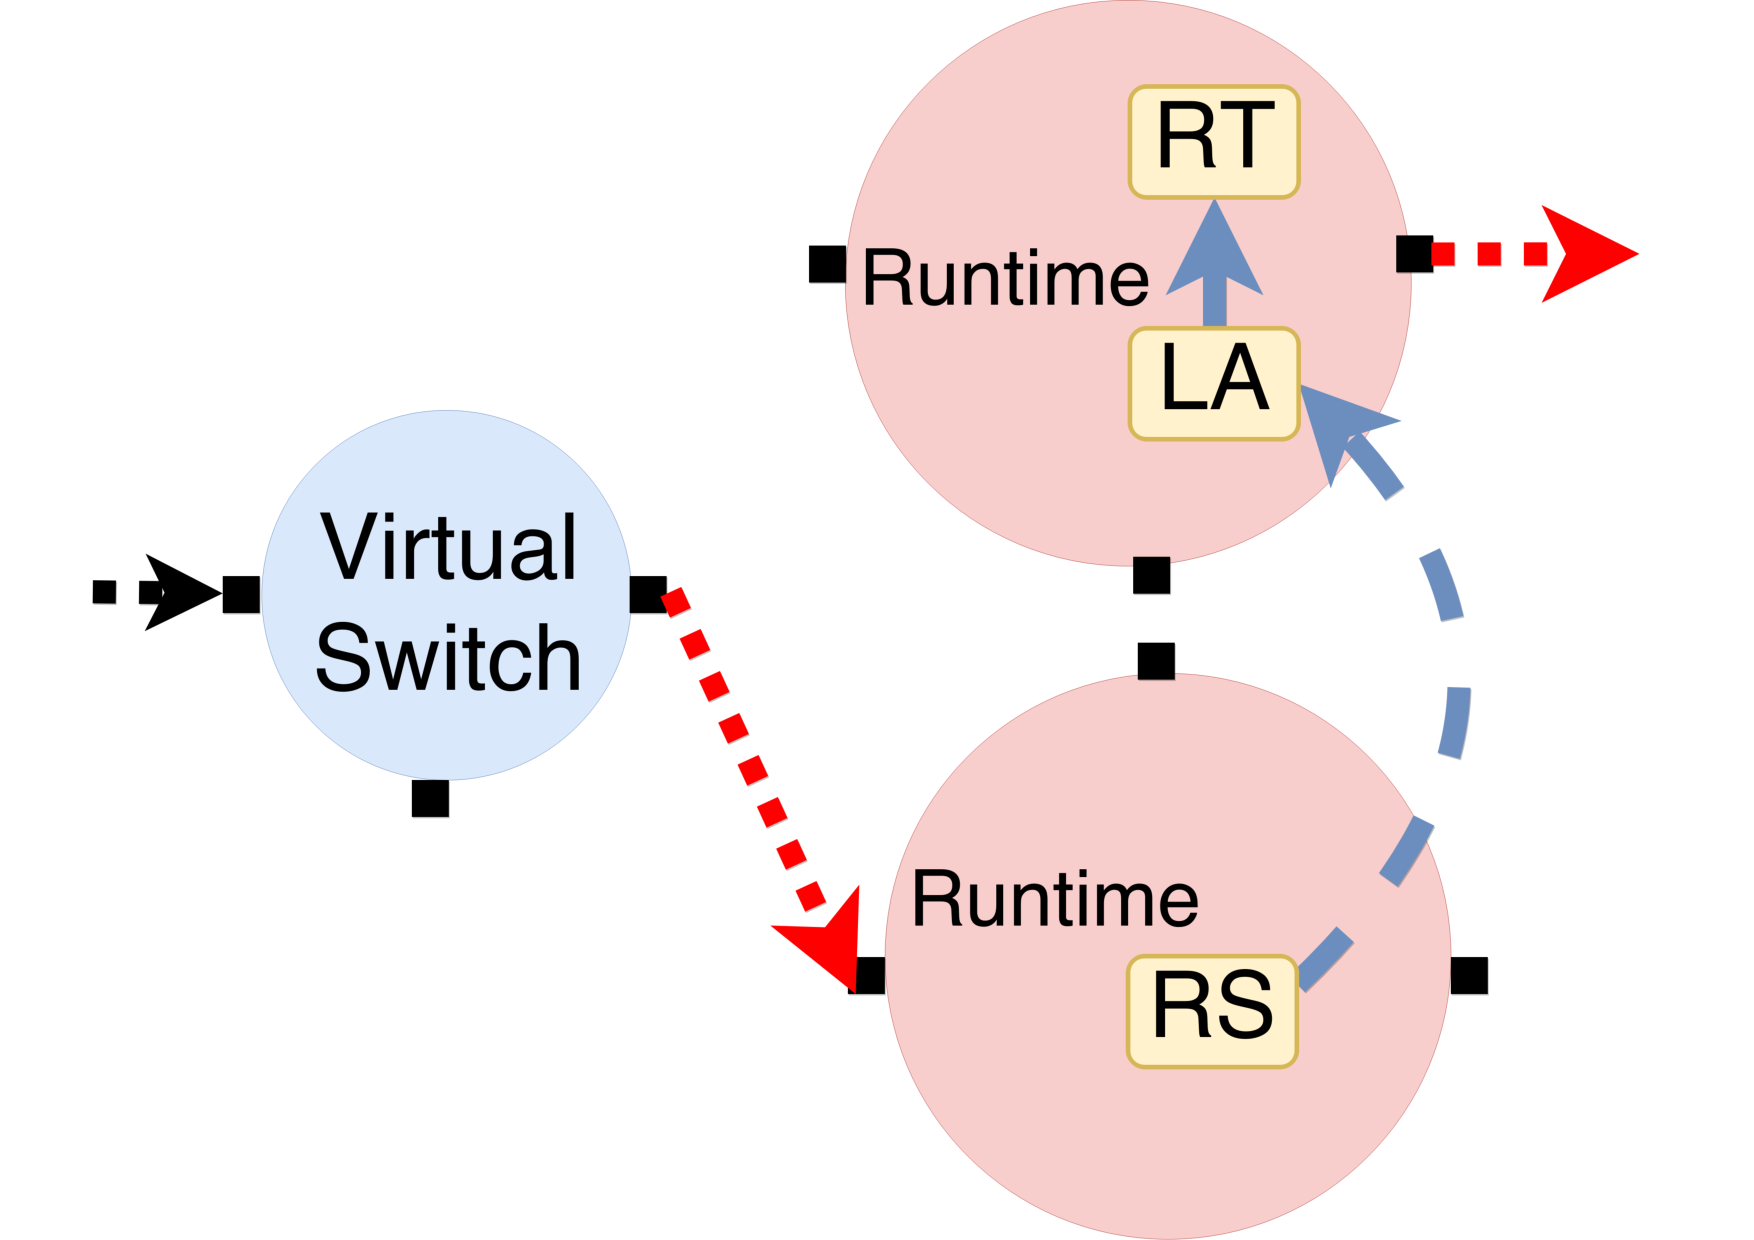
\includegraphics[width=\columnwidth]{chap-nfvactor/figure/nfactor-replication.pdf}
   \caption{Flow replication.}\label{fig:rep}
  \end{subfigure}
  \begin{subfigure}[t]{0.49\linewidth}
     \centering
     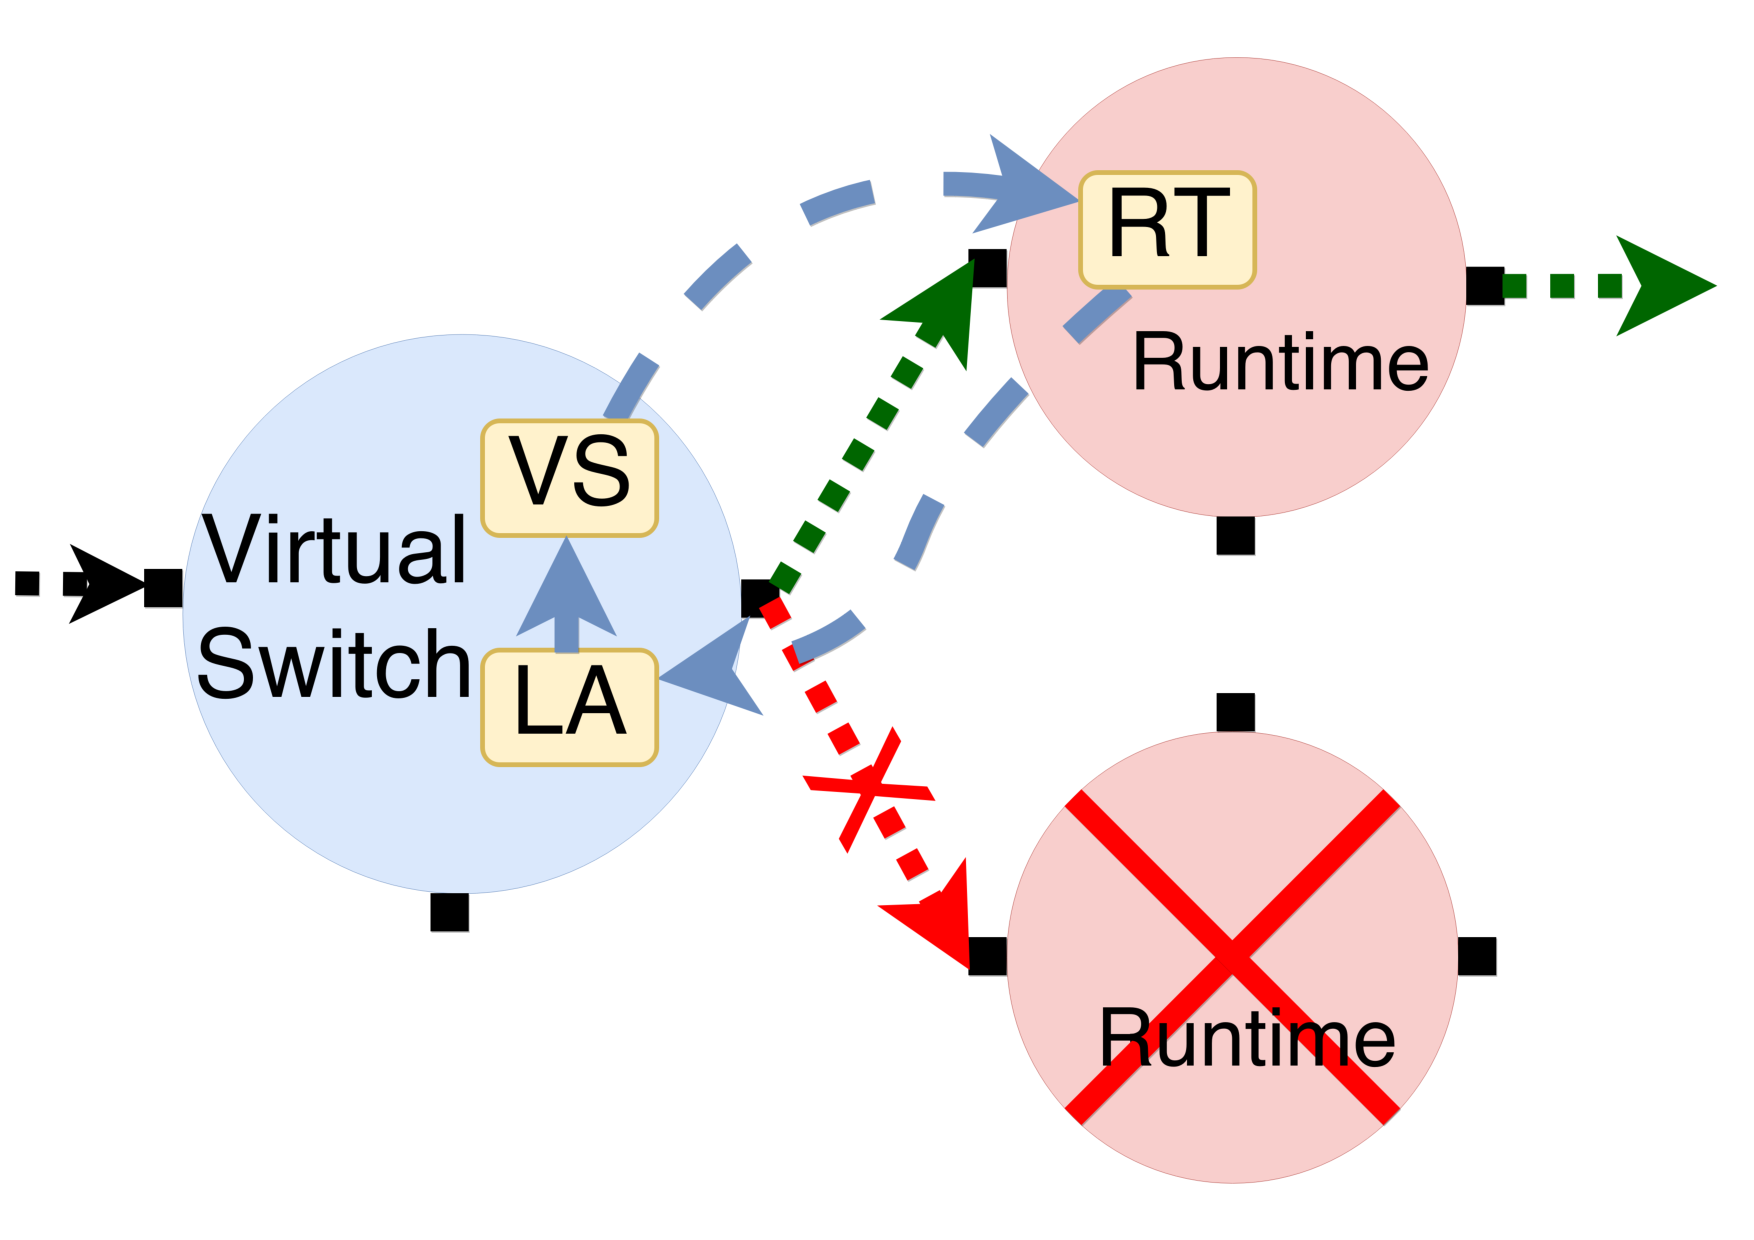
\includegraphics[width=\columnwidth]{chap-nfvactor/figure/nfactor-recover.pdf}
     \caption{Flow recover when the original runtime has failed.}\label{fig:recover}
    \end{subfigure}
 \caption{Flow replication and recovery: \textbf{RT} - replication target actor, \textbf{RS} - Replication source actor, \textbf{LA} - liaison actor, \textbf{VS} - virtual switch actor; \textbf{dotted line} - flow packets, \textbf{dashed line} - actor messages.)}
\label{fig:flow-rep}
\end{figure}

To perform lightweight runtime replication, we leverage the actor abstraction and state separation. In a runtime, important states associated with a flow are stored by the flow actor. The runtime can replicate each flow actor independently without check-pointing the entire container image \cite{sherry2015rollback, rajagopalan2013pico}. While achieving good throughput and fast flow recovery, this replication strategy also improves the packet processing delay and has good scalability, as each flow actor can replicate itself on another runtime without the need of dedicated back-up servers.

The detailed flow replication process is illustrated in Fig.~\ref{fig:flow-rep}. When a runtime is launched, the coordinator sends a list of runtimes in the same cluster to its liaison actor via RPC $set\_replicas(runtime\_id\_list)$. When a flow actor is created on the runtime, it acquires its replication target runtime from the liaison actor, selected in a round-robin fashion among all available runtimes received from the coordinator.

When a flow actor has finished processing a flow packet, it sends a replication actor message, containing the current flow states of all the NFs and the packet, directly to the liaison actor on the replication target runtime. The liaison actor further forwards the replication message to a replica flow actor sharing the same 5-tuple as the flow actor. The replica flow actor stores latest flow states contained in the message, and then directly sends the packet out, as shown in Fig.~\ref{fig:rep}. This design guarantees the same \textit{output-commit} property as in \cite{sherry2015rollback}: the packet is sent out from the system only when all the state changes caused by the packet have been replicated.

The coordinator monitors the liveness of a runtime by sending heartbeat messages to the liaison actor of the runtime. When a runtime fails, the coordinator sends recovery RPC requests $recover(runtime\_id) $ to all the runtimes containing replica flows of the failed runtime. When a runtime $R$ receives this RPC, it instructs each replica flow actor on runtime $R$ to send a request to the virtual switch actor, asking it to change the destination runtime to runtime $R$. After the acknowledge message from the virtual switch actor is received, the replica flow actor synchronizes the shared states by calling $flow\_recover$ (Table~\ref{table:api}) and the flow is successfully restored on runtime $R$ (Fig.~\ref{fig:recover}).

\subsubsection{Replicating Virtual Switches}

Since a virtual switch is in fact a special runtime (Sec.~\ref{sec:virtualswitch}), the virtual switch can be replicated in the same way as described in Sec.~\ref{sec:replicating-runtime}. The only difference is that when the source virtual switch fails, the replica flow actors in the replication target virtual switch immediately become the primary flow actors without sending out a request to change the forwarding route. Instead, the coordinator takes control and updates the SDN rules to forward the input flows to the replication target virtual switch.

\subsubsection{Replicating Coordinator}

Since the coordinator is a single-threaded module, we can log and replicate information it maintains into a reliable storage system such as ZooKeeper\cite{hunt2010zookeeper}. The liveness of the coordinator is monitored by a guard process and it is restarted immediately in case of failure. On a reboot, the coordinator can reconstruct the system view by replaying logs.

\subsection{Flow Migration}
\label{sec:migration}

\begin{figure}[!h]
\begin{subfigure}[t]{0.33\linewidth}
   \centering
   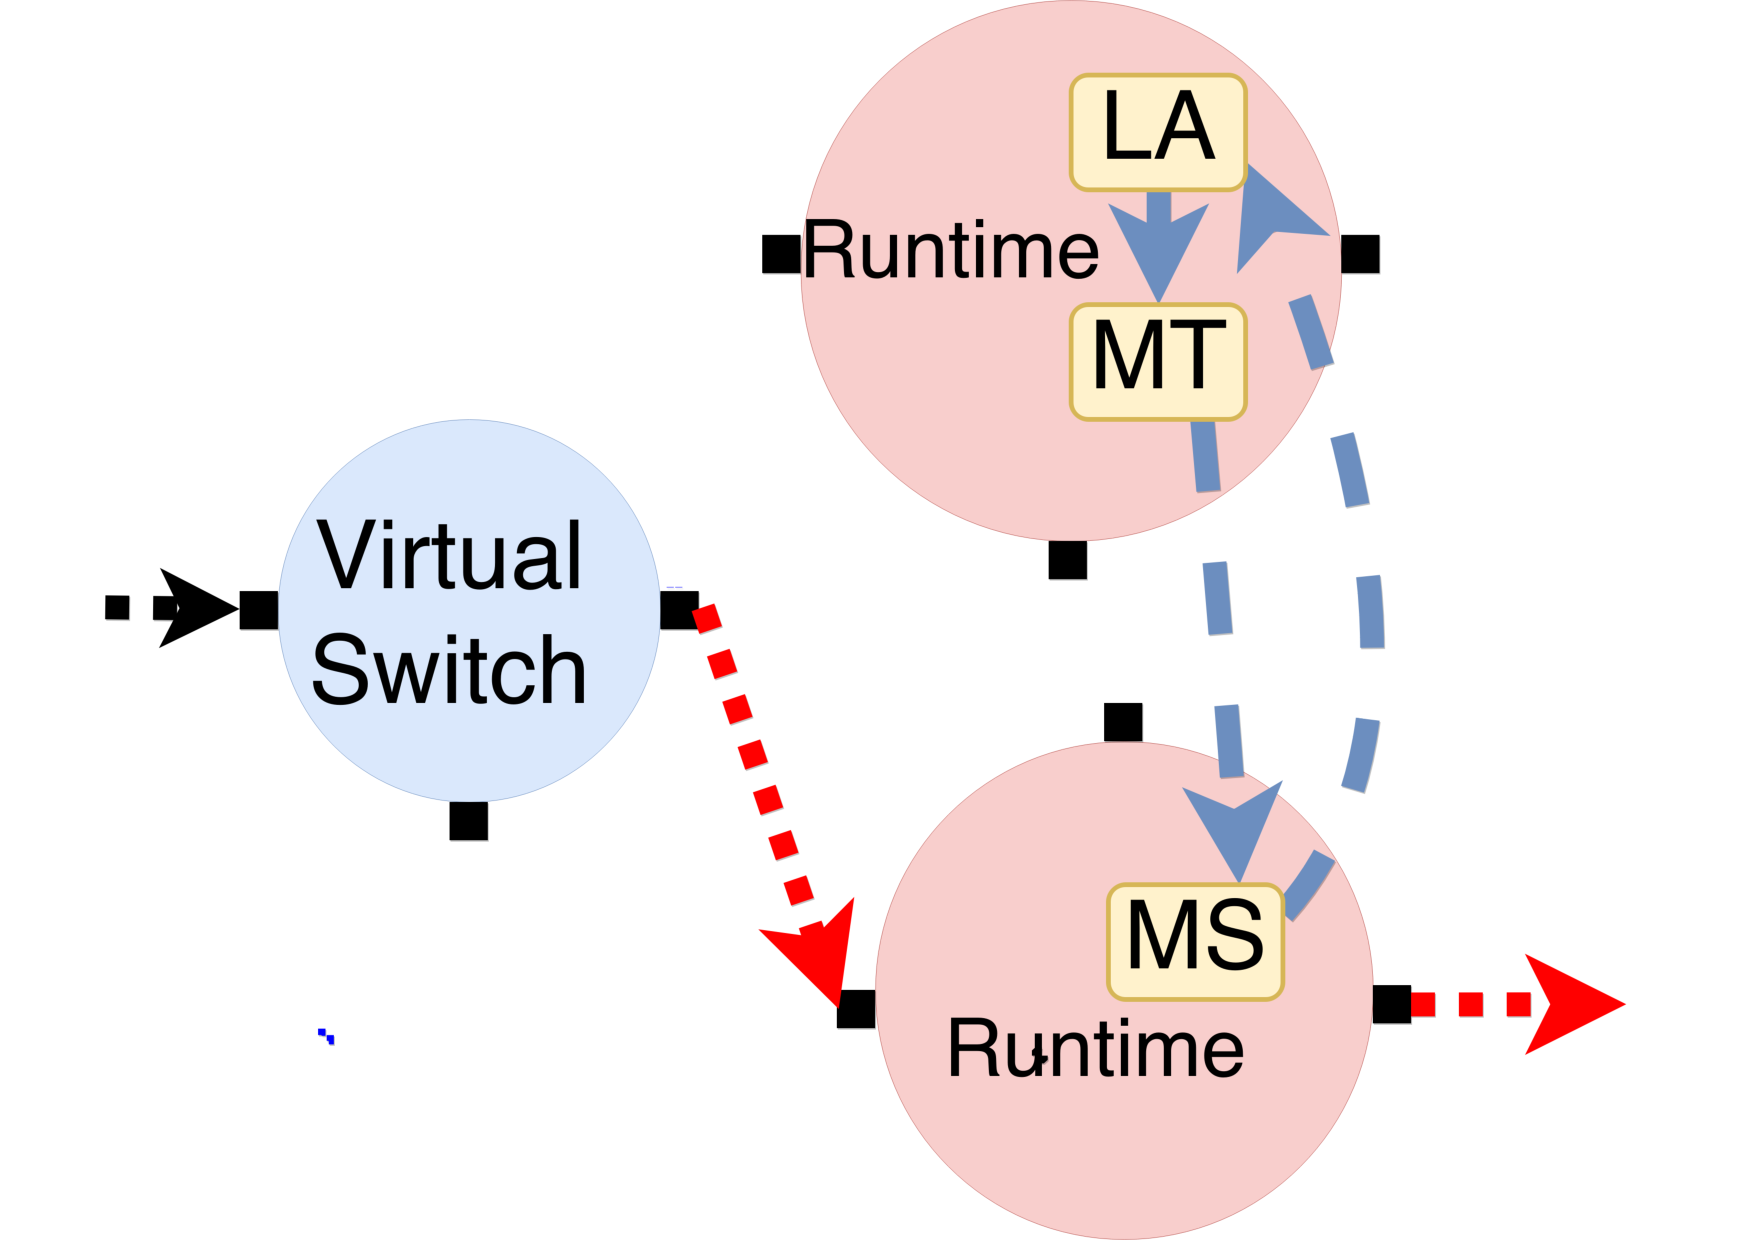
\includegraphics[width=1.1\columnwidth]{chap-nfvactor/figure/nfactor-mig1.pdf}
   \caption{1st req-rep step.}\label{fig:mig1}
  \end{subfigure}\hfill
  \begin{subfigure}[t]{0.33\linewidth}
     \centering
     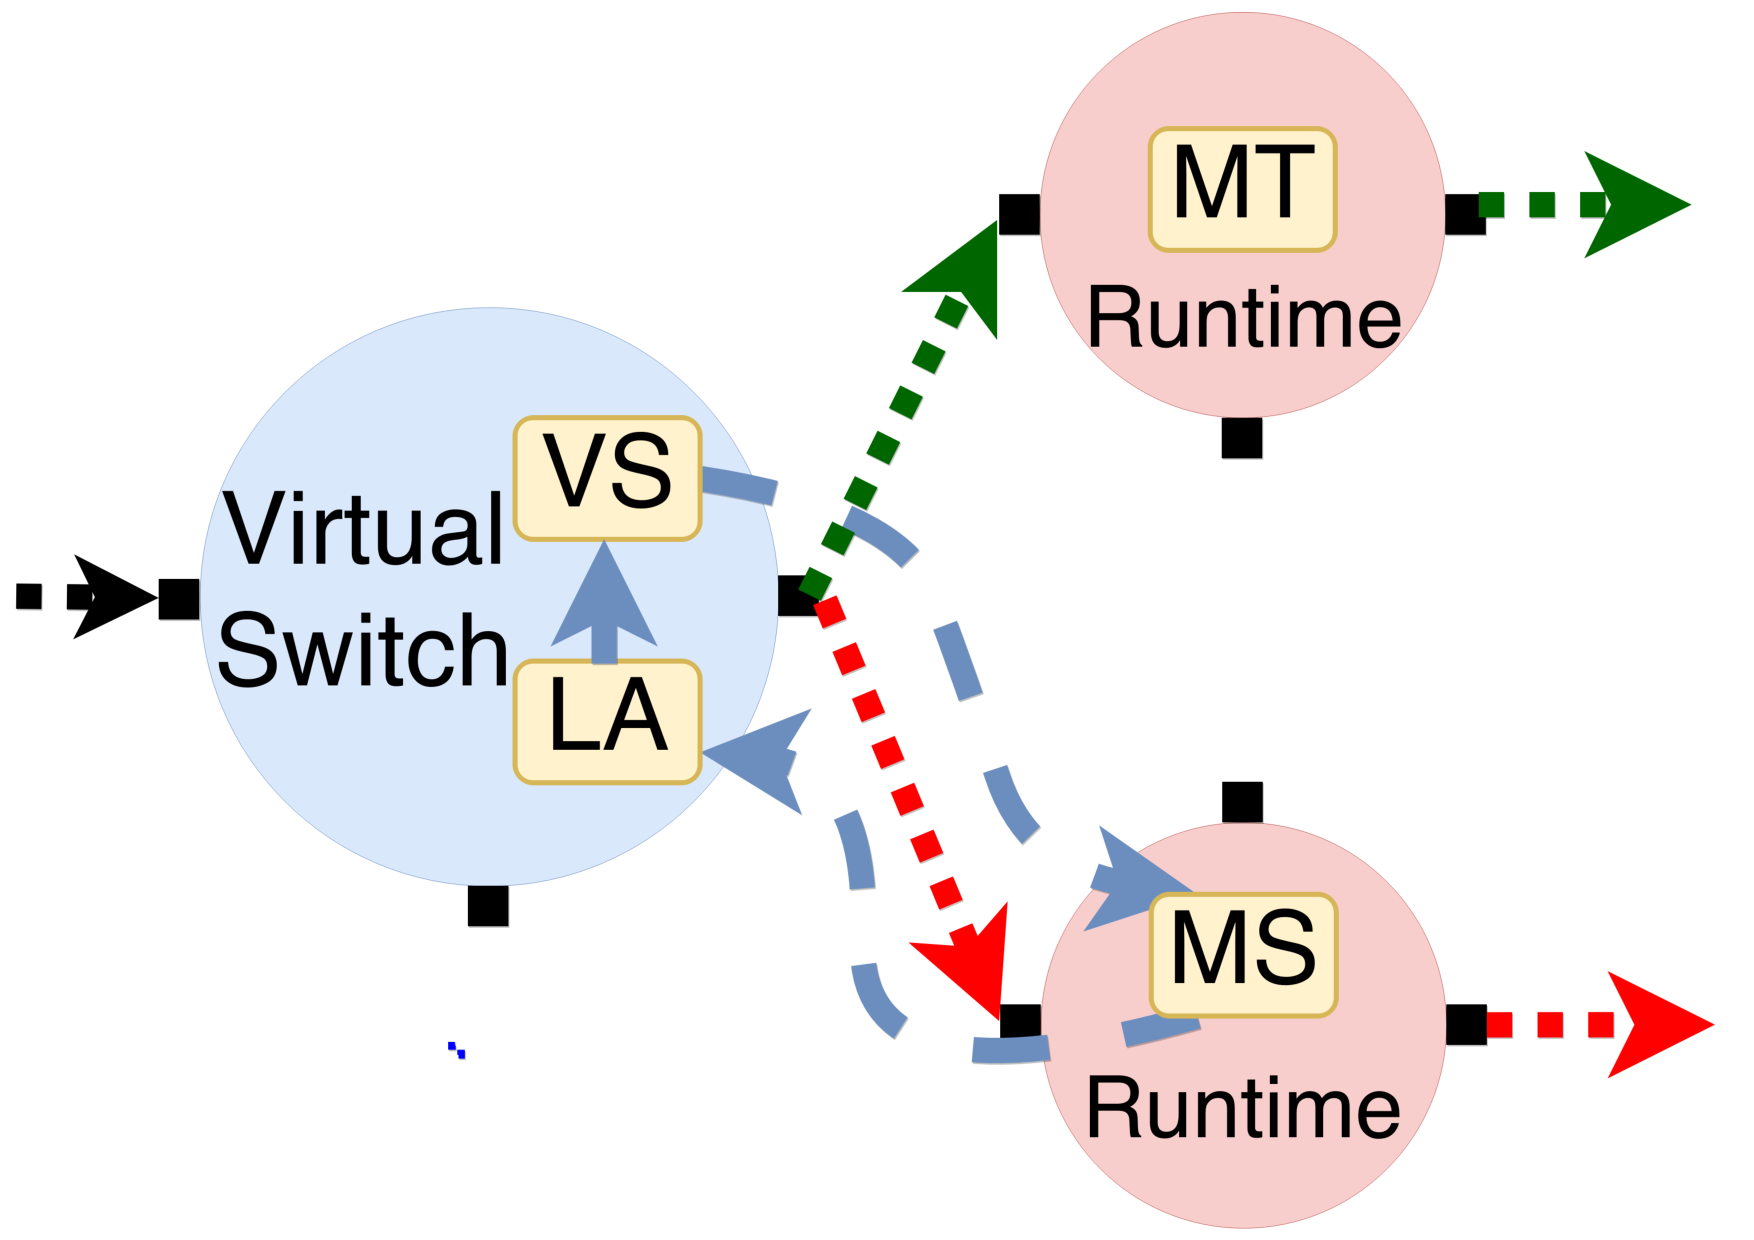
\includegraphics[width=1.1\columnwidth]{chap-nfvactor/figure/nfactor-mig2.pdf}
     \caption{2nd req-rep step.}\label{fig:mig2}
    \end{subfigure}\hfill
  \begin{subfigure}[t]{0.33\linewidth}
 \centering
   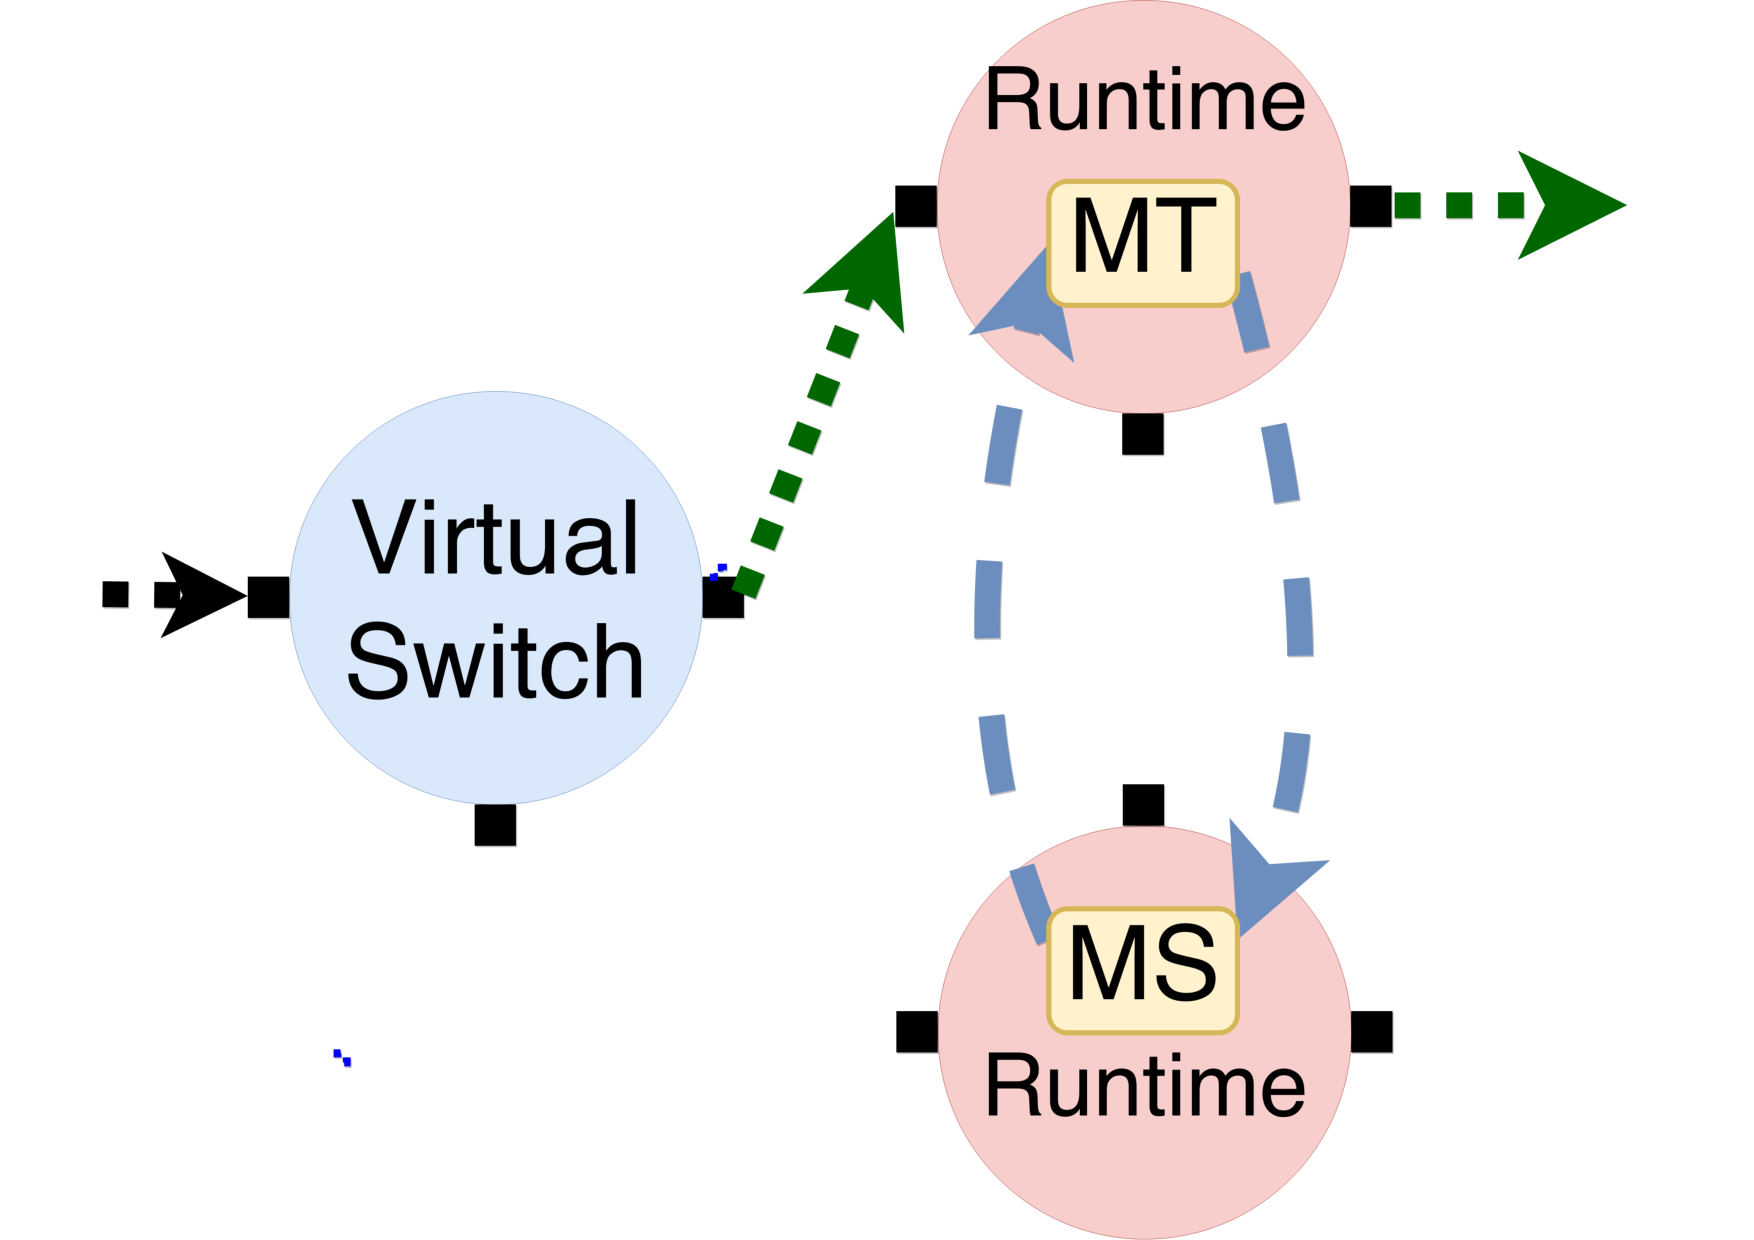
\includegraphics[width=1.1\columnwidth]{chap-nfvactor/figure/nfactor-mig3.pdf}
   \caption{3rd req-rep step.}\label{fig:mig3} \end{subfigure}\hfill
 \caption{The 3 flow migration steps: \textbf{MT} - migration target flow actor, \textbf{MS} - migration source flow actor, \textbf{LA} - liaison actor, \textbf{VS} - virtual switch actor; \textbf{dotted line} - flow packets, \textbf{dashed line} - actor messages.}
\label{fig:mig}
\end{figure}

Based on the actor model, flow migration in \nfactor~can be regarded as a transaction between a source flow actor and a target flow actor, where the source actor delivers its entire state and processing tasks to the target actor. Flow migration is successful once the target actor has completely taken over packet processing of the flow. In case of unsuccessful flow migration, the source flow actor can fall back to regular packet processing and instruct to destroy the target actor.

In \nfactor, the coordinator starts flow migration by calling $set\_migration\_target$ RPC method on a runtime, asking it to migrate a number of flows to another runtime. After receiving the ID of a migration target runtime, the flow actor starts migration by itself. The flow migration protocol used by flow actors is shown in Fig.~\ref{fig:mig}, consisting of three request-response steps. In case of request timeout, the migration source actor performs clean-up procedures and reverts to normal packet processing.

\textbf{1st req-rep step:} The source flow actor sends 5-tuple of its flow to the liaison actor on the migration target runtime. The liaison actor creates a migration target actor using the 5-tuple, and sends a response back to the migration source actor. Meanwhile, migration source actor continues to process packets as usual.

%\item
\textbf{2nd req-rep step:} The source flow actor sends the 5-tuple of its flow and the ID of the migration target runtime to the liaison actor on the virtual switch. The liaison actor uses the 5-tuple to identify the virtual switch actor in charge and notifies it to change the destination runtime to the migration target runtime. After this change, the virtual switch actor sends a response back to the source actor, and the migration target actor starts to receive packets. Instead of processing the packets, the target actor buffers all the received packets until it receives the request in the 3rd step from the source actor. The migration source actor keeps processing received flow packets until it receives the response from the virtual switch.

%\item
\textbf{3rd req-rep step:} The source flow actor sends its flow states to the migration target actor. After receiving the flow states, the migration target actor saves them, calls $flow\_migrate\_in$ (Table~\ref{table:api}) to synchronize the shared states, and immediately starts processing all the buffered packets while sending a response to the source actor. The migration source actor calls $flow\_migrate\_out$ (Table~\ref{table:api}) to synchronize the shared states and then destroys itself.

%\end{itemize}

{\em Loss Avoidance.} It is possible for our flow migration protocol to drop flow packets. However, packet drop caused by the flow migration protocol rarely happens in practice, even when concurrently migrating hundreds of thousands of flows (Sec.~\ref{sec:fmp}). We refer to this as loss-avoidance property, which is slightly weaker than the loss-free property \cite{gember2015opennf} in OpenNF.

In the 3rd step, before the request arrives at the migration target actor, the migration target actor has already received and buffered several flow packets. The buffer may overflow, causing migration target actor to drop several packets. However, our distributed flow migration finishes fast within several microseconds and such drop rarely happens in practice.
%\vspace{-1mm}

Still in the 3rd step, after the request is sent out by the source actor, it is possible for some flow packets to continue arriving at the source actor. These packets are sent out by the virtual switch actor before its destination runtime is changed in the 2nd step, but arrive later at the source actor than the response of the 2nd step. The source actor has to discard these packets because it has already sent out its flow state. ~\nfactor~minimizes the occurrence of this problem by having the virtual switch actor transmitting the response message of the 2nd step in the same network path as the flow packets, so that we rarely observe this problem in practice.
%\vspace{-1mm}

It has been a common understanding that providing good properties for flow migration would trade off the performance of flow migration \cite{gember2015opennf}. \nfactor~mitigates this trade-off using distributed, high-performance flow migration based on the actor model.

\section{Implementation}
 \label{sec:nfvactor-implementation}

\begin{figure}[!h]
\begin{subfigure}[t]{0.49\linewidth}
   \centering
   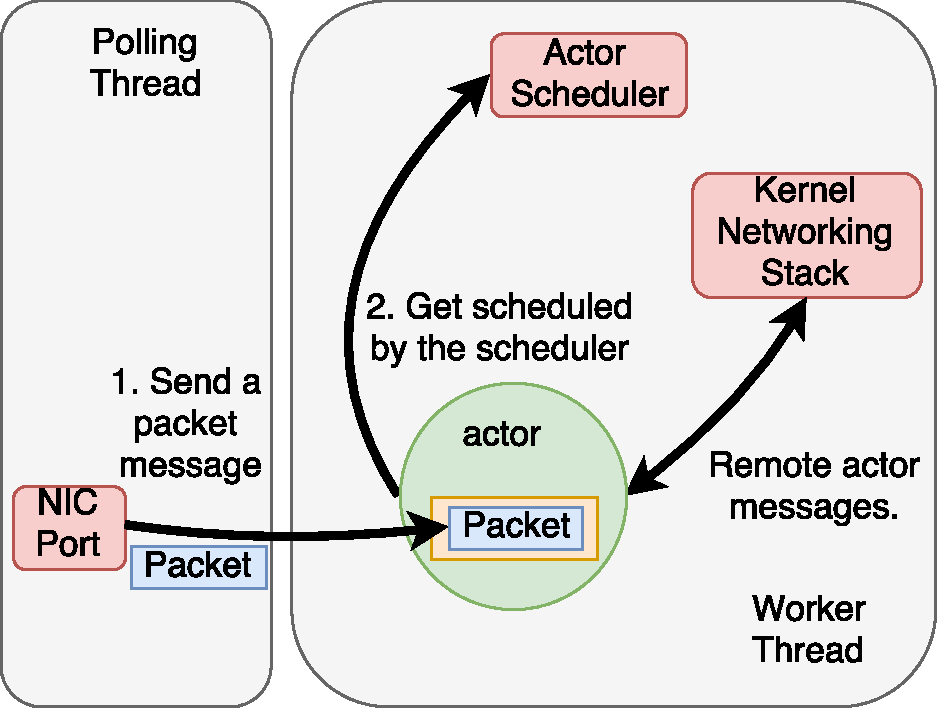
\includegraphics[width=\columnwidth]{chap-nfvactor/figure/actor-scheduling.pdf}
   \caption{Libcaf runtime.}\label{fig:actor-schedule}
  \end{subfigure}
  \begin{subfigure}[t]{0.49\linewidth}
     \centering
     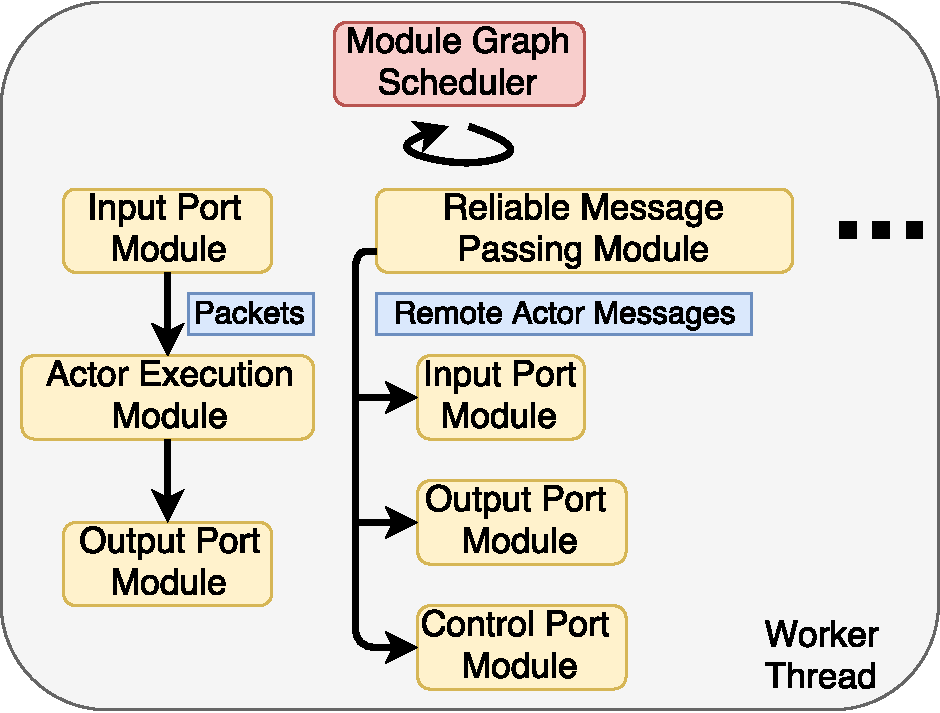
\includegraphics[width=\columnwidth]{chap-nfvactor/figure/graph-scheduling.pdf}
     \caption{\nfactor~runtime.}\label{fig:graph-schedule}
    \end{subfigure}
 \caption{Comparison of runtime architecture.}
\label{fig:two-versions}
\end{figure}

Throughout the development process of~\nfactor, we initially chose libcaf \cite{caf} as the runtime, whose architecture is shown in Fig.~\ref{fig:actor-schedule}. However, the performance of libcaf \cite{caf} runtime is less than satisfactory, for both packet processing and resilience operations. We believe that the performance problems of libcaf runtime come from two aspects. \textit{First}, the actor scheduler of libcaf is not suitable for handling IO of raw network packets. According to Fig.~\ref{fig:actor-schedule}, the scheduler schedules an actor run according to whether the actor has received a message. To inject dataplane packets into libcaf runtime, we have to set up a dedicated polling thread to poll the NIC port and send received packets to actors running in another worker thread by enqueueing the packet into actor's message queue. As verified in Sec.~\ref{sec:packet-processing-tl}, there is an expensive synchronization overhead between polling thread and worker thread, which may decrease packet processing throughput by over 100\%. \textit{Second}, libcaf runtime still relies on inefficient kernel networking thread to exchange remote actor messages with other runtimes.

Realizing these problems, we design a customized actor runtime for \nfactor~as shown in Fig.~\ref{fig:graph-schedule}, by leveraging two optimizations. \textit{First}, we implement a module graph scheduler to schedule actors according to several pre-defined module graphs. The module graph scheduler combines various IO operations (polling NIC port, exchanging remote actor messages) with actor scheduling inside a single worker thread, effectively eliminating the thread synchronization overhead as in libcaf. \textit{Second}, we bypass inefficient kernel networking stack and implement a high-performance, reliable message passing module running in user-space.

The tradeoff point when designing the customized runtime is programmability, as the programming interface exposed by the customized runtime is not as easy to use as the libcaf runtime. However, we believe that such a tradeoff is worthwhile due to improved performance.

% The~\nfactor~is implemented by about 8500 lines of code in C++, except the code for NFs. The implementation of \nfactor~has gone through a few trials and errors. Initially, we used libcaf \cite{caf} and implemented a runtime as shown in Fig.~\ref{fig:actor-schedule}. Even though libcaf is probably the fastest existing actor library \cite{chs-rapc-16}, performance of the first version is less than satisfactory, primarily due to the inefficacy of message passing through concurrent message queue and relying on kernel network stack for remote actor message transmission. The problems motivated us to design a customized actor library for \nfactor~and implement a new runtime as shown in Fig.~\ref{fig:graph-schedule}.

%\vspace{-2mm}
%\subsection{Customized Actor Library}

%We adopt three optimization strategies in our actor library to speed up packet processing. First, concurrent message queue is removed from each actor and message passing is transformed into direct function call. Second, in libcaf, an actor is scheduled to run after a message is placed into its message queue. Due to the first optimization, our library cannot follow libcaf's scheduling strategy. Instead, we implement a module graph scheduler to schedule actors according to several pre-defined module graphs (Sec.~\ref{sec:mgs}). Third, we bypass the kernel network stack and implement a reliable message passing module (Sec.~\ref{sec:rmp}) running in user-space.

\noindent \textbf{Module Graph Scheduler.} Inspired by the scheduler design of BESS \cite{bess} and Click \cite{kohler2000click}, the module graph scheduler keeps scheduling several module graphs to run in a round-robin fashion. A module graph consists of several processing modules, connected together into an acyclic graph. Inside a module graph, the actor messages are generated by a source module, flow through the connected module for processing before reaching the sink module, which consumes each message by either freeing it or sending it to the outside. Inside a module, the message handler of the corresponding actor is called for each actor message. The actor then pushes the processed message to the next connected module. When all the generated actor messages are consumed, the scheduler moves on to run the next module graph. % The module graph can be implemented as a function call graph, fulfilling our goal of removing actor queues.

Fig.~\ref{fig:graph-schedule} illustrates two module graphs. The first module graph polls dataplane packets from the input port and generates packet messages, which are pushed along the module graph, processed by the flow actors and sent out from the output port. The second module graph fetches remote actor messages from the reliable message passing module and sends the remote actor message out from one of the three ports. There are two other module graphs that are used for receiving reliable actor messages and interacting with the RPC requests.

% The idea of module graph was originally introduced in the Click modular router \cite{kohler2000click} and then extended by BESS \cite{bess}. However, we are the first to apply module graph scheduling to speed up actor processing.

%Remote actor messages passed among different runtimes should be reliably delivered.
\noindent \textbf{Reliable Message Passing.} Based on the module graph scheduler, we build a reliable message passing module, which inserts remote actor messages into a reliable packet stream for transmission. The module creates one ring buffer for each remote runtime and virtual switch. When a flow actor on this runtime sends a remote actor message, the module creates a packet, copies the content of the message into the packet and then enqueues the packet into the respective ring buffer. These packets are configured with a sequential number each, and appended with a special header to differentiate them from dataplane packets. When the second module graph in Fig.~\ref{fig:graph-schedule} is scheduled to run, the worker thread dequeues these packets from the ring buffers, and sends them to respective remote runtimes. A remote runtime acknowledges receipt of such packets. Retransmission is fired in case that the acknowledgement for a packet is not received after a configurable timeout (\eg, 10 times the RTT in our current implementation). Running entirely in user-space, the performance of the reliable message passing module is good enough to saturate a 10Gbps link (Sec.~\ref{sec:srram}).

Since our goal is to reliably transmit remote actor messages over an inter-connected L2 network, we do not use user-level TCP \cite{jeong2014mtcp}, which may impose additional overhead for reconstructing byte streams into messages. In addition, packet-based reliable message passing provides additional benefits during flow migration and replication. Because the response in 2nd request-response step of flow migration is sent as a packet using the same path as the dataplane packets, reliable actor message passing enables us to implement loss-avoidance migration with ease (Sec.~\ref{sec:migration}).



%Since our goal is to reliably transmit remote actor messages over an inter-connected L2 network, we do not use user-level TCP \cite{jeong2014mtcp}, which may impose much more processing overhead for reconstructing byte streams into messages. %In addition, packet-based reliable message passing provides additional benefits during flow migration and replication. Because the response in 2nd request-response step of flow migration is sent as a packet using the same path as the dataplane packets, reliable actor message passing enables us to implement loss-avoidance migration with ease (Sec.~\ref{sec:migration}).

\section{Evaluation}
\label{sec:experiments}


We evaluate \nfactor~using 4 Dell R430 servers, each equipped with an Intel Xeon E5-2650 CPU running at 2.30GHz with 20 logical CPU cores, 48GB memory and 2 Intel X710 10Gb NICs. The servers are connected through a 10GB Dell switch. In each server, the worker thread of each runtime is pinned to a dedicated logical core, while the RPC threads of all the runtimes are collectively pinned to logical core 0 to minimize the performance impact on the worker thread. To generate test traffic, we use a customized traffic generation module (the FlowGen module) of BESS \cite{bess}, which is capable of generating input traffic up to 10Gbps (at around 14Mpps) with 64-byte packets.

We use a single server to generate the traffic. We set up 6 virtual switches on another server, which are capable of handling input traffic at 10Gbps line rate and do not render bottlenecks. The rest of the servers are used to run runtimes.

\subsection{Performance of the Runtime}
\label{sec:micro-benchmark}

\begin{figure}[!h]
  \begin{subfigure}[t]{0.49\linewidth}
    \centering
    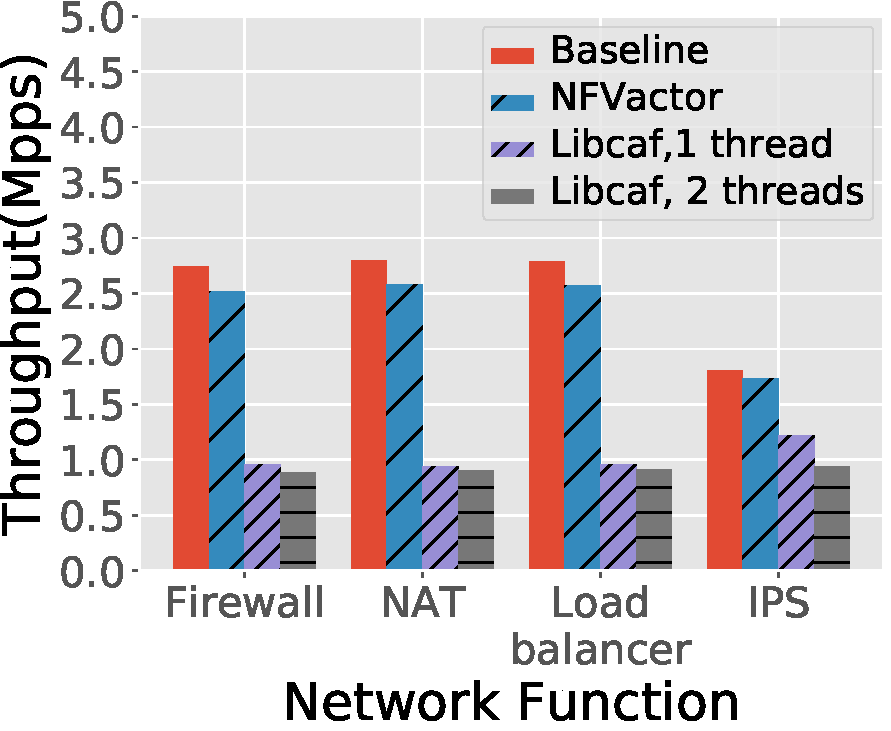
\includegraphics[width=\columnwidth]{chap-nfvactor/exp-figure/micro_throughput.pdf}
    \caption{}\label{fig:micro_throughput}
  \end{subfigure}\hfill
  \begin{subfigure}[t]{0.49\linewidth}
    \centering
    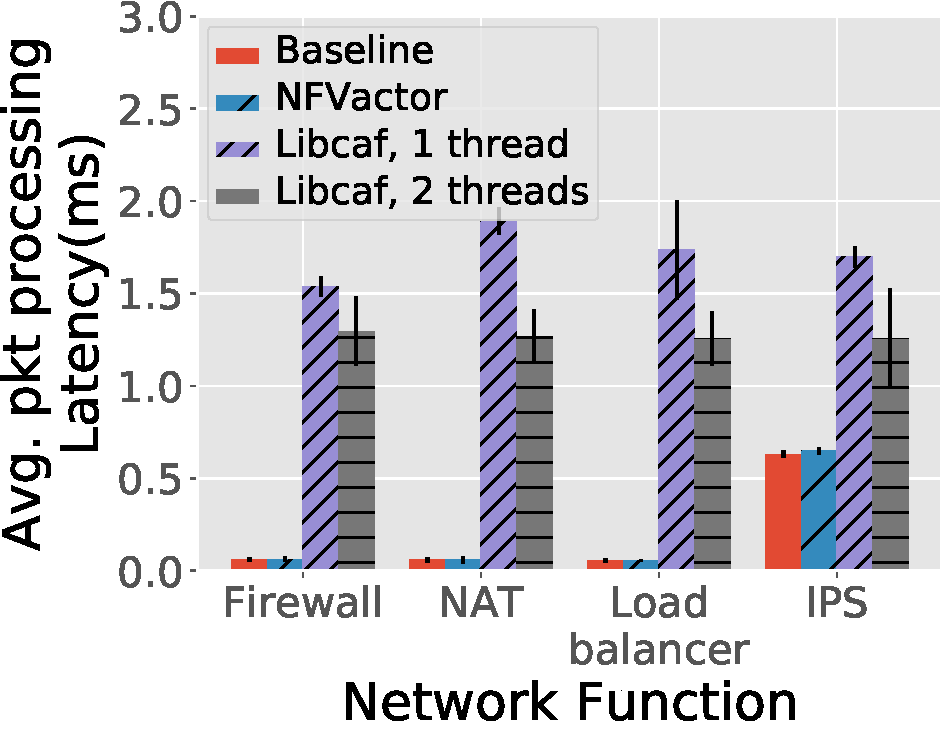
\includegraphics[width=\columnwidth]{chap-nfvactor/exp-figure/micro_latency.pdf}
    \caption{}\label{fig:micro_latency}
  \end{subfigure}\hfill
  \begin{subfigure}[t]{0.49\linewidth}
    \centering
    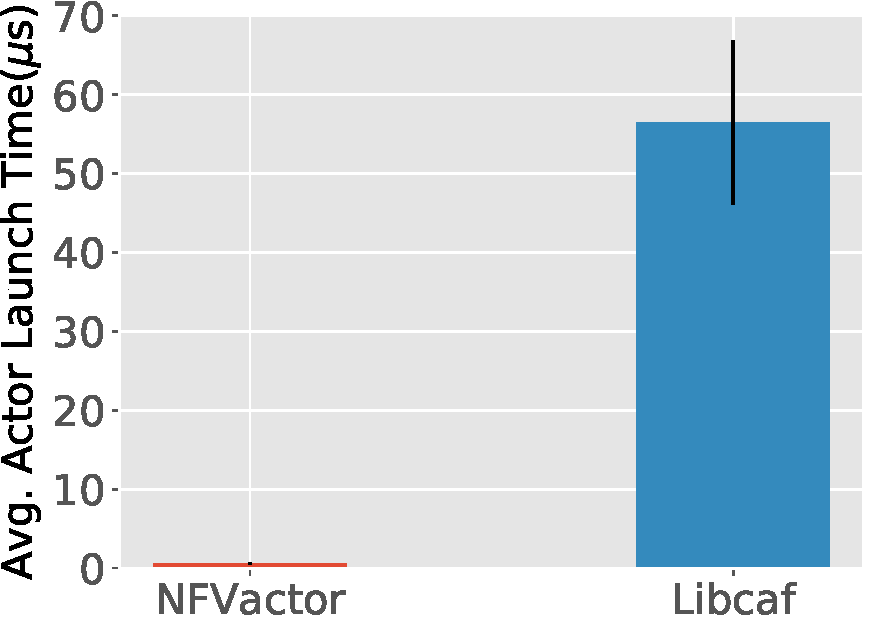
\includegraphics[width=\columnwidth]{chap-nfvactor/exp-figure/micro_launch_time.pdf}
    \caption{}\label{fig:micro_launch_time}
  \end{subfigure}\hfill
  \begin{subfigure}[t]{0.49\linewidth}
    \centering
    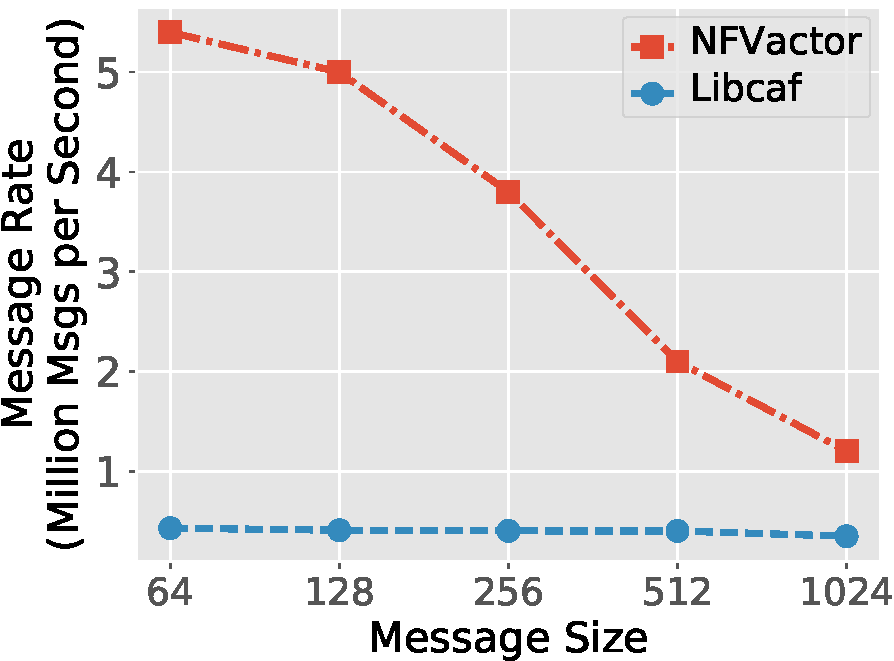
\includegraphics[width=\columnwidth]{chap-nfvactor/exp-figure/micro_mp.pdf}
    \caption{}\label{fig:micro_mp}
  \end{subfigure}
\caption{Performance of the Runtime.}
\end{figure}

\subsubsection{Packet processing throughput and latency}
\label{sec:packet-processing-tl}

We first evaluate the packet processing throughput (number of packets processed per second) and latency (difference between the time that a packet enters the runtime to the time this packet is released from the runtime) of the \nfactor~runtime by running the four implemented NFs. The traffic generator produces flows with 64-byte TCP packets, a 10pps (packets per second) flow rate and a 10-second active time. The overall packet rate of the input traffic is 5Mpps. For comparison, we also evaluate performance of libcaf runtime. We vary the number of worker threads used by the libcaf runtime to reflect the performance overhead of thread synchronization. Finally, we compare with four baseline NFs. The baseline NFs are implemented using a normal packet processing loop, sharing similar processing logic as the $process\_pkt$ API. The per-flow state in each baseline NF is stored in a fast hash table \cite{pagh2001cuckoo} without using the actor abstraction.

Fig.~\ref{fig:micro_throughput} and Fig.~\ref{fig:micro_latency} show that \nfactor~runtime achieves significantly larger throughput and smaller processing latency than libcaf runtime, and the performance of the NFs in~\nfactor~is close to that of the baseline NFs, as the actor abstraction does introduce a small overhead. According to Fig.~\ref{fig:micro_throughput}, when the number of the worker threads used by libcaf is increased, the total throughput drops by a small margin, due to increased synchronization overhead between the polling thread and multiple worker threads.



\subsubsection{Actor launch time and sending rate of remote actor messages}
\label{sec:srram}

The actor launch time is the time when the first packet of a flow is received to the time when this packet is processed by the launched actor. It is a strong performance indicator of the actor runtime system. In Fig.~\ref{fig:micro_launch_time}, the input traffic is the same as in Sec.~\ref{sec:packet-processing-tl}. We see that the average actor launch time in \nfactor~is much smaller than that of the libcaf runtime, as \nfactor~pre-allocates flow actors into a ring buffer to speed-up actor launch time.

Fig.~\ref{fig:micro_mp} shows the average sending rate of remote actor messages between two runtimes running on different servers. For various message sizes, the message rate achieved by~\nfactor~is significantly larger than that of libcaf. Especially, when the message size is larger than 256 bytes, we measure the consumed bandwidth of~\nfactor~to be around 9.1Gbps, which is close to the 10Gbps line rate. This result reflects that our user-space message passing module can significantly improve the performance of remote actor communication.

%When the size of each remote actor message is smaller than 128 bytes, the message rate is limited by about 5M messages (the worker thread's limitation decided by the CPU frequency), and the line speed is not reached; when the size of each remote actor message is larger than 256 bytes, the worker thread only needs to send out a smaller number of messages while saturating the line speed. In contrast, with libcaf, the messaging rate is limited by the bottleneck of enqueuing and dequeuing messages to a broker thread \cite{caf}, and the line speed cannot be approached.

\subsection{System Scalability}
\label{sec:ppt}

\begin{figure}[!h]
  \begin{subfigure}[t]{0.49\linewidth}
    \centering
    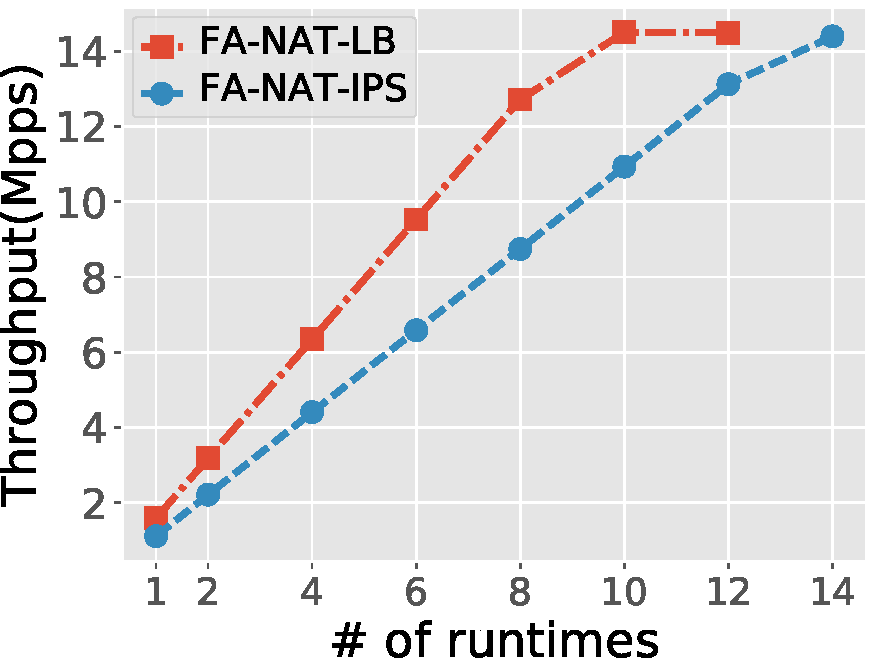
\includegraphics[width=\columnwidth]{chap-nfvactor/exp-figure/throughput_scaling.pdf}
    \caption{}\label{fig:throughput_scaling}
  \end{subfigure}\hfill
  \begin{subfigure}[t]{0.49\linewidth}
   \centering
   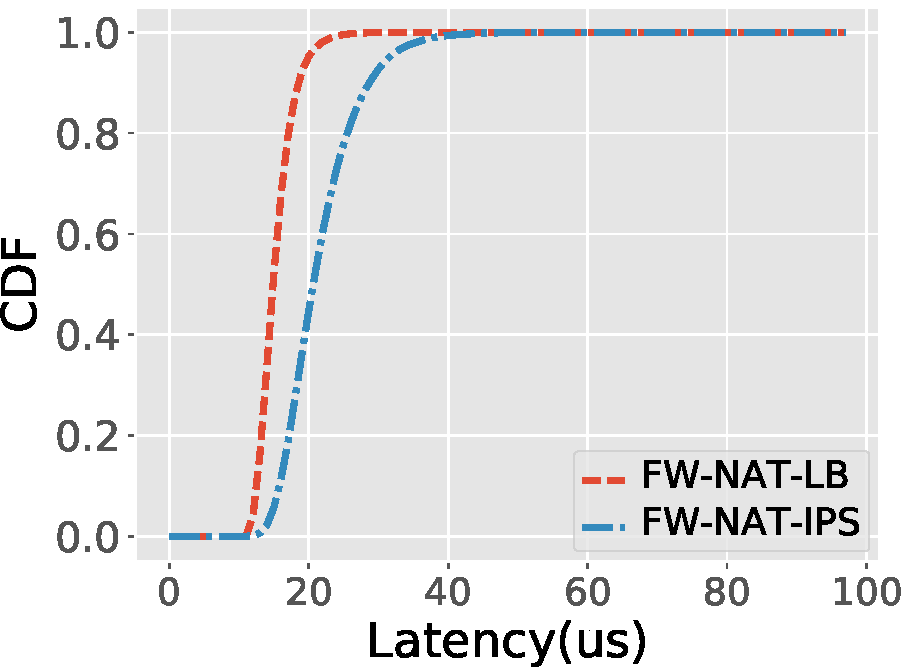
\includegraphics[width=\columnwidth]{chap-nfvactor/exp-figure/throughput_latency_cdf.pdf}
   \caption{}\label{fig:throughput_latency_cdf}
  \end{subfigure}\hfill
  \begin{subfigure}[t]{0.49\linewidth}
   \centering
   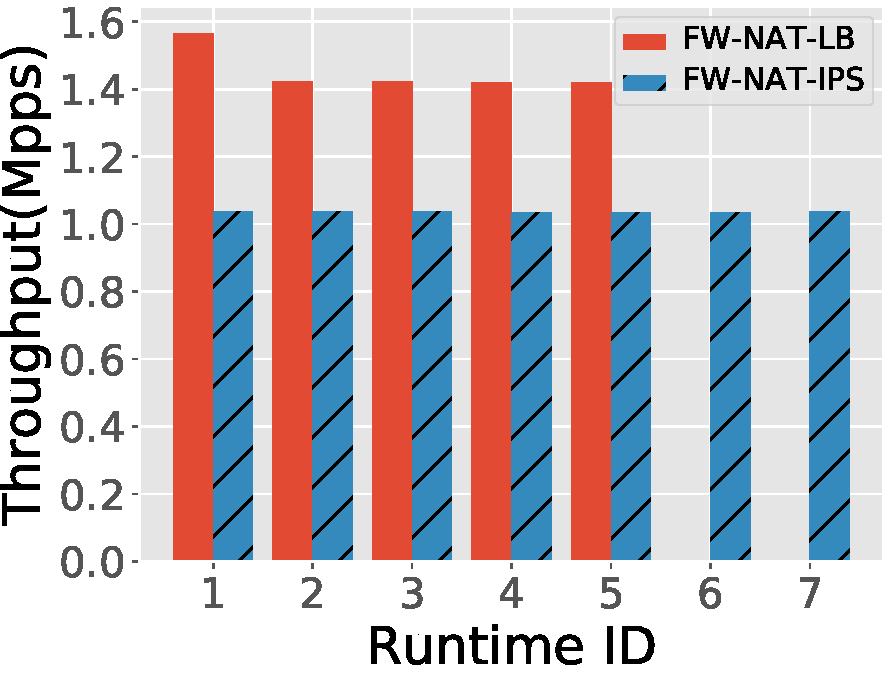
\includegraphics[width=\columnwidth]{chap-nfvactor/exp-figure/throughput_2sc.pdf}
   \caption{}\label{fig:throughput_2sc}
  \end{subfigure}
  \begin{subfigure}[t]{0.49\linewidth}
    \centering
    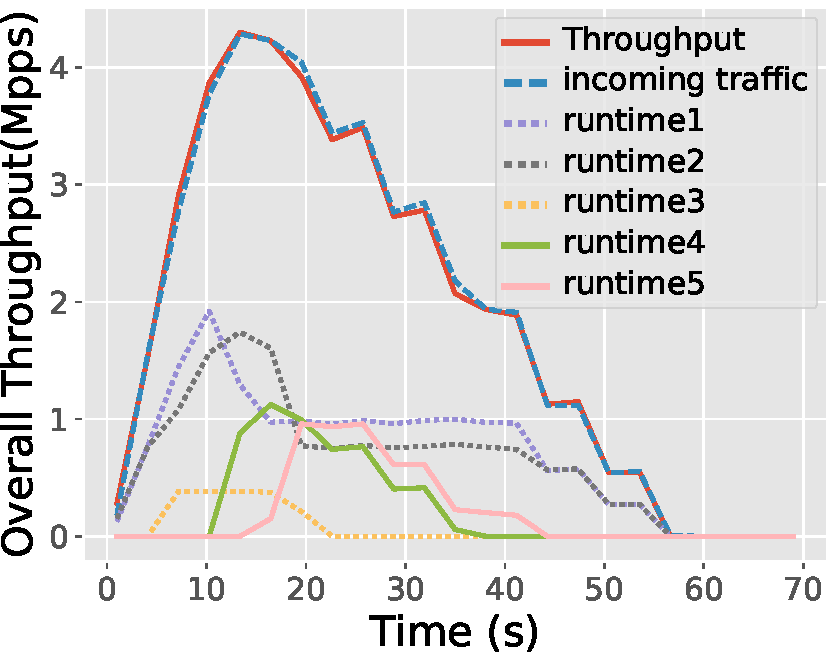
\includegraphics[width=\columnwidth]{chap-nfvactor/figure/Scale.pdf}
    \caption{Dynamic scaling.}\label{fig:scale}
  \end{subfigure}\hfill
\caption{System scalability.}
\end{figure}

We now evaluate the maximum packet processing throughput of \nfactor~as the number of runtimes increases. We use two servers and configure the runtimes with service chain `firewall (FW) $\rightarrow$ NAT $\rightarrow$ load balancer (LB)' (in one set of experiments) or service chain `firewall (FW) $\rightarrow$ NAT $\rightarrow$ IDS' (in another set of experiments). To fully stress the system, we configure traffic generators to produce a mixture of short flows and long flows up to 10Gbps line rate. A short flow consists of 64-byte TCP packets with a 10pps packet rate and lasts for 1 second. A long flow consists of 64-byte TCP packets with a 10pps packet rate and lasts for 10 seconds. Each type of flow consumes half of generated bandwidth. We gradually increase the number of active runtimes and collect the total throughput achieved by the runtimes.

Fig.~\ref{fig:throughput_scaling} shows the overall packet processing throughput increases linearly with the increase of the runtimes. Overall throughput of 14.49Mpps (9.70Gbps) and 14.39Mpps (9.67Gbps) are achieved when the runtimes run service chain `FW $\rightarrow$ NAT $\rightarrow$ LB'and `FW $\rightarrow$ NAT $\rightarrow$ IDS', respectively.
This verifies that~\nfactor~can approach 10Gbps line-rate packet processing for 64-byte small packets, even when the input traffic consists of many short-lived flows. %We believe that~\nfactor~can handle 10Gbps line-rate with fewer runtimes if the input traffic has less short-lived flows.

Fig.~\ref{fig:throughput_latency_cdf} shows the CDF of packet processing latencies, collected during a 20s period when 10 and 14 runtimes are used to run `FW $\rightarrow$ NAT $\rightarrow$ LB' and `FW $\rightarrow$ NAT $\rightarrow$ IDS', respectively. The average latency for both service chain is around 20$\mu$s.

We next run the two service chains concurrently in the system. We run 5 runtimes in one server configured with `FW $\rightarrow$ NAT $\rightarrow$ LB' and 7 runtimes in another server configured with `FW $\rightarrow$ NAT $\rightarrow$ IDS'. The input traffic has a total packet rate of 14.50Mpps and shares the same mixed pattern to produce Fig.~\ref{fig:throughput_scaling}. The input traffic is evenly split among the two service chains. Fig.~\ref{fig:throughput_2sc} shows the throughput of each runtime. We can see that a total throughput of 7.25Mpps can be reached by each service chain. The workload is also evenly balanced among runtimes in the same server, demonstrating the effectiveness of our virtual switches for load balancing under mixed short and long flows.

Finally, the performance of the dynamic scaling controlled by the coordinator is shown in Fig.~\ref{fig:scale}. The traffic generator generates traffic with increasing packet rate for the first 15 seconds, and then gradually decreases the packet rate of the traffic for the last 45 seconds. %A total number of 100K flows is generated throughout the experiment.
The cluster is initialized with two runtimes (runtime 1 and 2) running `FW $\rightarrow$ NAT $\rightarrow$ IDS' service chain. Starting from the 10th second, runtimes 1 and 2 become overloaded and their workload is gradually migrated away to runtime 4 and 5. With dynamic scaling, the achieved throughput can correctly match the input traffic during the 60 seconds.

\subsection{Performance of Flow Replication}
\label{sec:rp}

\begin{figure}[!h]
 \begin{subfigure}[t]{0.49\linewidth}
		\centering
		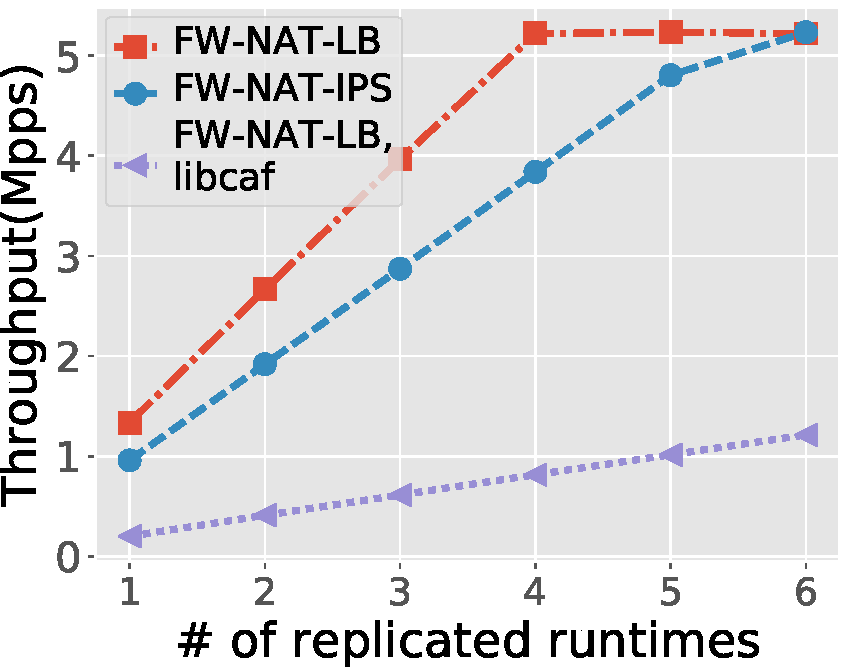
\includegraphics[width=\columnwidth]{chap-nfvactor/exp-figure/rep_scaling.pdf}
		\caption{}\label{fig:rep_scaling}
	 \end{subfigure}\hfill
	 \begin{subfigure}[t]{0.49\linewidth}
	\centering
		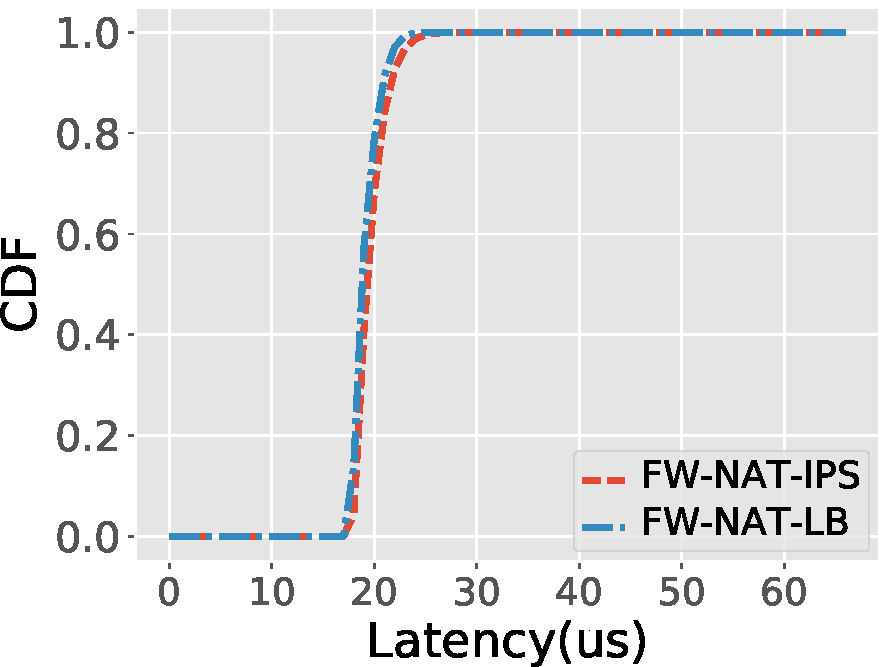
\includegraphics[width=\columnwidth]{chap-nfvactor/exp-figure/rep_latency_pdf.pdf}
		\caption{}\label{fig:rep_latency_pdf} \end{subfigure}
	\caption{Performance of flow replication.}
\label{fig:rep-perf}
\end{figure}

\begin{table}[!h]
\centering
\caption{Recovery time and \# of flows recovered}
\vspace{-3mm}
\label{table:recover}
\resizebox{\columnwidth}{!}{
\begin{tabular}{|l|l|l|l|}
\hline
                                                                                   & FW$\rightarrow$NAT$\rightarrow$LB          & FW$\rightarrow$NAT$\rightarrow$IDS            & FW$\rightarrow$NAT$\rightarrow$LB, libcaf           \\ \hline
\begin{tabular}[c]{@{}l@{}}Average recovery time\\ for each runtime\end{tabular}   & 65.3ms             & 66.6ms             & 934.2ms           \\ \hline
\begin{tabular}[c]{@{}l@{}}Number of flows recovered\\ on each runtime\end{tabular} & at least 87k flows & at least 87k flows & at least 20k flows \\ \hline
\end{tabular}
}
\vspace{-3mm}
\end{table}

In this set of experiments, input flows are produced following the same mixed pattern to produce Fig.~\ref{fig:throughput_scaling}. The coordinator chooses two servers and launches the same number of runtimes on them. The coordinator instructs each runtime on a server to replicate its flows to a distinct runtime in another server. We gradually increase packet rate of the input traffic and the number of runtimes running on each server, to investigate throughput and scalability when flow replication is enabled.

Fig.~\ref{fig:rep_scaling} shows that both service chains can scale up to handle the 5.22Mpps input packet rate when six runtimes running on a server concurrently replicate their traffic to six replica runtimes on another server. In particular, when the input rate reaches 5.22Mpps, the measured bandwidth on the link for transmitting replication messages reaches almost 10Gbps. When the libcaf version of implementation is used, the replication throughput is significantly lower.

Fig.~\ref{fig:rep_latency_pdf} shows the CDF of packet processing latencies of \nfactor~when flow replication is enabled. The latency measured in this experiment is difference between the time that the packet enters replication source runtime to the time this packet is released from the replication target runtime. For both service chains, the number of runtimes on each of the two servers is 6 while the input packet rate is 5.22Mpps. The average latency is around 20$\mu$s for both service chains.

Table \ref{table:recover} shows the average recovery time of 6 replication target runtimes when their corresponding replication source runtimes fail simultaneously. We can see that \nfactor~has a much shorter recovery time than the libcaf version even when processing a larger number of flows.

\vspace{-3mm}
\subsubsection{Comparison with FTMB} We compare the performance of flow replication in \nfactor~with the reported performance of FTMB \cite{sherry2015rollback}. Both systems achieve throughput up to millions of packets per second and recovery time of tens of milliseconds with flow replication enabled. \nfactor~has a more stable packet processing latency (according to Fig.~\ref{fig:rep_latency_pdf}, smaller than 70 microseconds, with an average of 20 microseconds) because it does not need to checkpoint the runtime, whereas FTMB introduces a relatively high packet processing latency (up to 3000 microseconds) when checkpointing kicks in.

\subsection{Performance of Flow Migration}
\label{sec:fmp}

\begin{figure}[!h]
 \begin{subfigure}[t]{0.49\linewidth}
   \centering
   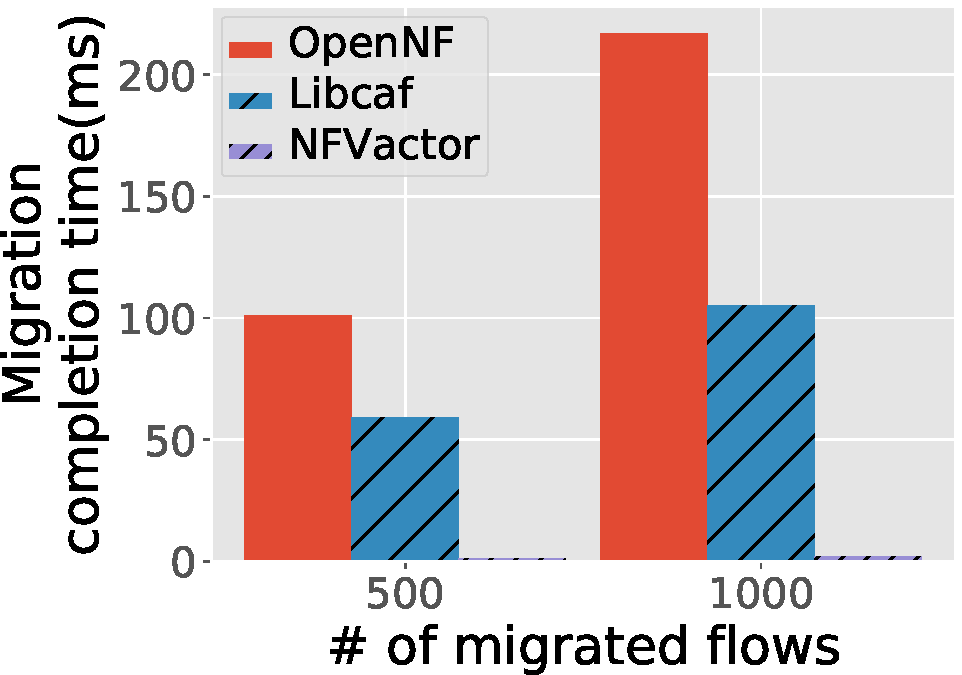
\includegraphics[width=\columnwidth]{chap-nfvactor/exp-figure/migration_compare.pdf}
   \caption{}\label{fig:migration_compare} \end{subfigure}\hfill
  \begin{subfigure}[t]{0.49\linewidth}
   \centering
   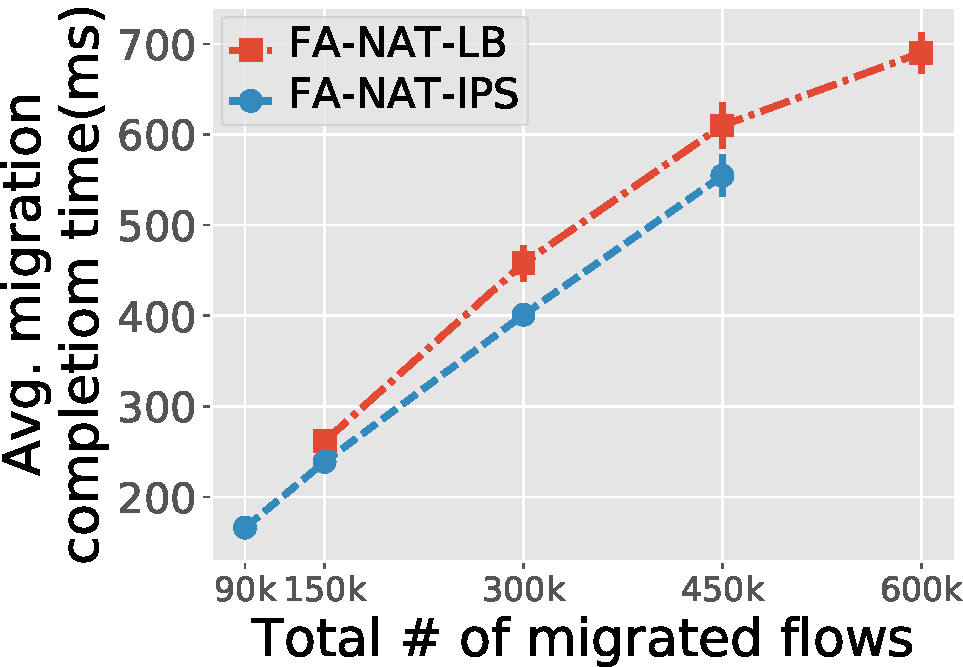
\includegraphics[width=\columnwidth]{chap-nfvactor/exp-figure/migration_time.pdf}
   \caption{}\label{fig:migration_time}
  \end{subfigure}
\caption{Flow migration completion time.}
\end{figure}

We first compare flow migration performance among \nfactor, libcaf runtime, and OpenNF. Both \nfactor~and libcaf runtime run the example firewall. We also port the example firewall to work with OpenNF. We send the same number of flows to the three firewalls and each flow has a 10pps packet rate. In Fig.~\ref{fig:migration_compare}, the time to migrate the respective number of flows is much smaller with \nfactor~(0.7ms for 500 flows and 1.5ms for 1000 flows), when compared to OpenNF (101ms for 500 flows and 217ms for 1000 flows) and the libcaf runtime (59ms for 500 flows and 105ms for 1000 flows). Due to efficient runtime design, \nfactor~can out-perform OpenNF by 144 times when migrating 1000 flows.

%To inspect performance of flow migration in \nfactor,
We next show the time taken for concurrently migrating a large number of flows among multiple pairs of runtimes. The traffic generator produces a number of flows with a 10pps flow rate, each lasting for 1 minute. The flows are first sent to three runtimes running in one server. Then the coordinator instructs the three runtimes to concurrently migrate all the flows to three runtimes running in another server. %This experiment tests the same service chain configurations as in Sec.~\ref{sec:ppt} and the number of flows injected to each runtime is varied.

Fig.~\ref{fig:migration_time} shows the average migration completion time of the three migration source runtimes. The standard deviation of the completion time is shown as error bar in Fig.~\ref{fig:migration_time} as well. \nfactor~can migrate 600K flows (with 6Mpps total throughput) from three migration source runtimes running in one server to three migration target runtimes running in another server using around 700ms. Besides the performance boost enabled by efficient runtime design, the decentralized flow migration also contributes to the performance. Since the flow migration are concurrently carried out among three pairs of runtimes, each pair of runtime only needs migrates around 200K flows. This significantly reduce the eventual flow migration completion time for all the 600K flows. If the 600K flows are sequentially migrated, the resulted flow migration completion time may be prolonged to over 2 seconds. Finally, throughout the evaluation in Fig.~\ref{fig:migration_time}, we observe zero packet loss caused by our flow migration protocol.
%All these factors verify the effectiveness and robustness of our decentralized flow migration design.

% it takes 400-500ms to migrate 100k flows (with 1Mpps total throughput) on a single runtime, making flow migration a practical approach to resolve hot spots. Considering flow migration is concurrently carried out between three pairs of runtimes, it also demonstrates efficiency of our distributed flow migration protocol. In our experiments, we also observe no packet loss is caused by flow migration, validating the loss-avoidance property.

\begin{comment}
\subsection{Other Applications}
\label{sec:applications}

\begin{figure}[!h]
  \begin{subfigure}[t]{0.49\linewidth}
   \centering
   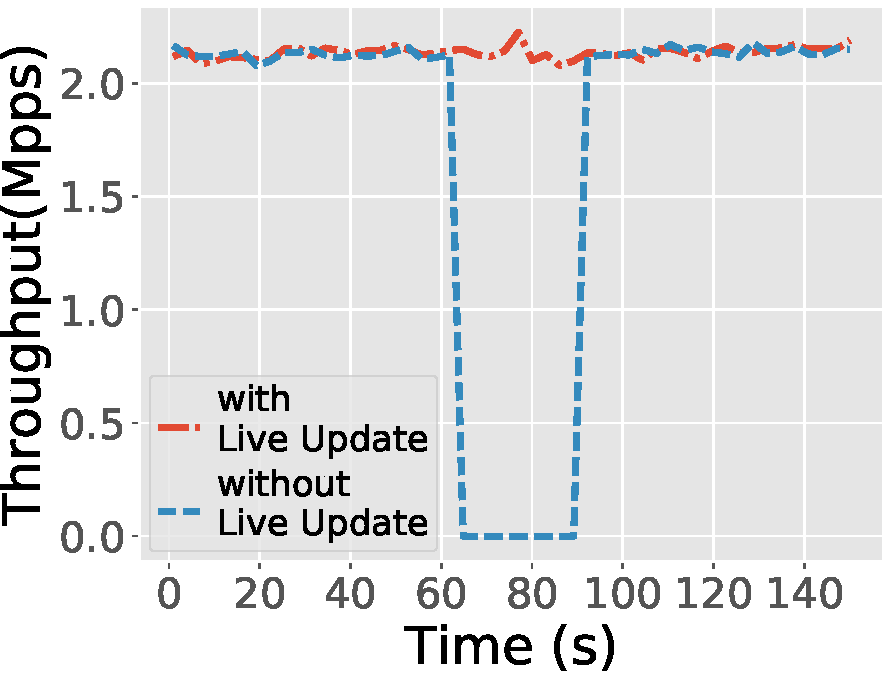
\includegraphics[width=\columnwidth]{figure/Dynamic.pdf}
   \caption{Live NF update.}\label{fig:dynamic}
  \end{subfigure}\hfill
  \begin{subfigure}[t]{0.49\linewidth}
   \centering
   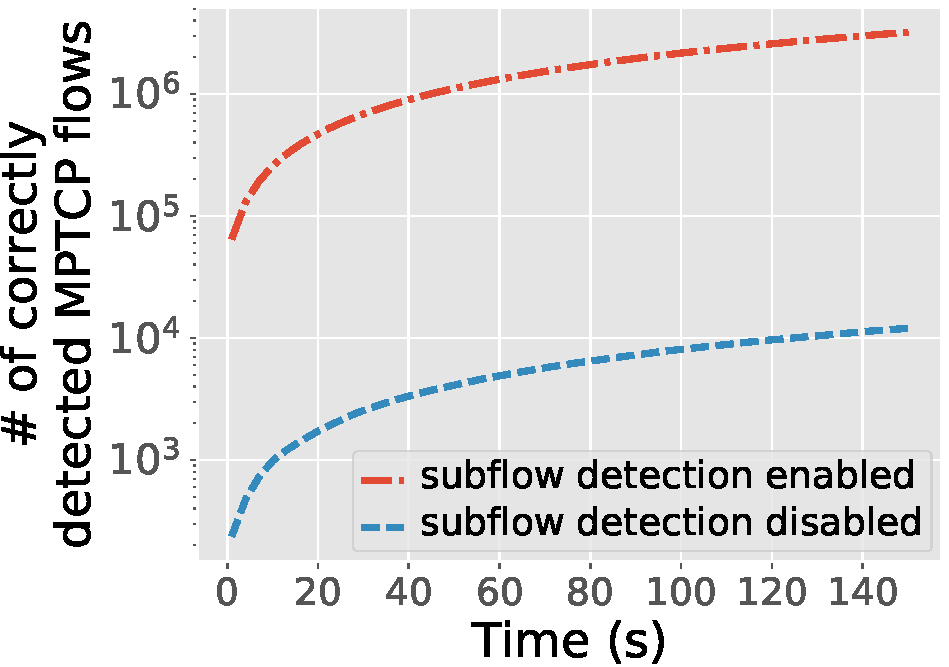
\includegraphics[width=\columnwidth]{figure/Mptcp.pdf}
   \caption{MPTCP subflow detection.}\label{fig:mptcp}
  \end{subfigure}
  \vspace{-2mm}
\caption{Other applications.}
\vspace{-4mm}
\end{figure}

In addition, we build two applications based on \nfactor, which exploit its lightweight, distributed flow migration capability to achieve useful functionalities.

\vspace{1mm}
\noindent\textbf{Live NF update.} \nfactor~can achieve dynamic NF update (\eg, software version, important NF configuration files) without interfering with active flows, by dynamically migrating the flows out to a replica runtime, performing update and migrating the flows back. Fig.~\ref{fig:dynamic} illustrates the throughput of a runtime running a firewall NF, during dynamic update of its firewall rule. No active flows are dropped during the update with \nfactor, while significant throughput drop occurs if shutting down the firewall for its update.

\vspace{1mm}
\noindent\textbf{MPTCP sub-flow processing.} When an MPTCP \cite{wischik2011design} flow traverses an NFV system, its sub-flows may be sent to different NF instances for processing. However, some NFs require all subflows to be processed by the same instance, \eg, IDS \cite{snort}. In \nfactor, we create a new NF for MPTCP sub-flows detection. Whenever the flow actor processes the first packet of a flow with this NF, the NF checks whether it belongs to an MPTCP flow. If so, the NF performs a consistent hashing using the MPTCP header to decide a migration target runtime in the cluster, and notify the flow actor to migrate itself to the target. In this way, different sub-flows belonging to the same MPTCP flow can be processed by the same flow actor. In existing flow migration systems, it is hard to incorporate sub-flow detection directly into the NFs: the NFs lack per-flow execution environment as in~\nfactor~and they can not initiate flow migration by themselves without instructions from the centralized controller.

In the experiment of Fig.~\ref{fig:mptcp}, we inject a total number of about 3.2M MPTCP flows to 3 runtimes. With subflow detection enabled, the total number of correctly processed MPTCP flows, \ie, those whose subflows are all processed by the same runtime, is always the same as the total number of input MPTCP flows. Without this detection, most of the subflows are processed by different runtimes.
\end{comment}

\section{Related Work}
\label{sec:relatedwork}

Since the introduction of NFV \cite{nfv-white-paper}, a broad range of studies have been carried out, for bridging the gap between specialized hardware and network functions \cite{hwang2015netvm, Han:EECS-2015-155, martins2014clickos, 199352}, scaling and managing NFV systems \cite{gember2012stratos, palkar2015e2}, flow migration \cite{rajagopalan2013split, khalid2016paving, gember2015opennf}, NF replication \cite{rajagopalan2013pico, sherry2015rollback}, and traffic steering \cite{simplifying}. In these work, NF instances are typically created as software modules running on separate VMs or containers. \nfactor~customizes a runtime system to run flow actors and embeds service chain processing within the flow actor abstraction, to achieve transparent and highly efficient failure resilience guarantee.


Among the existing studies, StatelessNF \cite{201545} shares similar design goals with~\nfactor, \ie, to enable transparent system scalability and failure resilience. However, the methodology used by StatelessNF is orthogonal to that of~\nfactor: it stores flow states in a reliable database \cite{ongaro2011fast} to achieve failure resilience, while~\nfactor~exploits the actor model. Compared with StatelessNF,~\nfactor~can approach line-rate packet processing and does not rely on RDMA equipment.

Besides, the Click modular router \cite{kohler2000click} is the first work to introduce modular design for simplifying NF construction.~The module graph scheduler used by~\nfactor~is partially inherited from the scheduler of Click. However,~\nfactor~uses such a scheduler to speed up actor processing. Flurries \cite{zhang2016flurries} proposes fine-grained per-flow NF processing, by dynamically assigning a flow to a lightweight NF. Sharing some similarities, \nfactor~enables micro service chain processing of each flow in one actor, but focuses on providing transparent failure tolerance based on the actor model. OpenBox \cite{OpenBox} merges the processing logic of multiple VNFs, therefore improving the modularity and processing performance. Even though \nfactor~uses the traditional sequential service chain, we believe that the flexibility of actor model can help us adopt the idea of OpenBox in \nfactor, which we leave for future exploration. StateAlyzr \cite{khalid2016paving} uses static analysis to automate flow state extraction and simply human effort for enabling flow migration. However, enabling high-performance flow migration still requires a holistic design like~\nfactor.

%while \nfactor~focuses on mainstream service chain processing and leaves this to future work.

%Even though the service chain concept has been expanded to service graphs in E2 \cite{palkar2015e2} and OpenBox \cite{OpenBox}, \nfactor uses the traditional service chain to process a flow as it still represents the mainstream processing method \cite{hwang2015netvm, martins2014clickos}.

%Compared with OpenNF \cite{gember2015opennf}, the flow migration completion time is improved by a large margin. Compared with FTMB \cite{sherry2015rollback},~\nfactor~achieves similar replication throughput and recovery time, while exhibiting a more stable end-to-end delay.

%To implement flow migration, existing systems \cite{gember2015opennf}\cite{rajagopalan2013split} require direct modification of the core processing logic of NF software, and mostly rely on an SDN controller to carry out migration protocol, involving non-negligible overhead. %message passing overhead that lowers packet processing speed of the system.
%Finally, the migration process is fully controlled by a  centralized SDN controller, which may not be scalable if there are many NF instances that need flow migration service.
%\nfactor~overcomes these issues using novelly designed NF APIs and a largely distributed framework, where flow states are easily extractable and migration is achieved directly in-between runtimes with only 3 steps of request-response. % and clean separation between NF processing logic and resilience enabling functionalities, as well as a system design based on the distributed actor framework.
%The actors can be migrated by communicating among themselves without the coordination from a centralized controller. A fast virtual switch is designed to achieve the functionality of a dedicated SDN switch. Only 3 rounds of request-response are needed for achieving flow migration, based on the actor framework and the customized virtual switch, enabling fast flow migration and high packet processing throughput.

%Flow replication to provide failure tolerance usually involves check-pointing the entire NF process image, % (where the NF software is running),
%and replica creation using the image \cite{sherry2015rollback,rajagopalan2013pico}. Temporary pause of an NF process is typically needed \cite{sherry2015rollback}, resulting in packet losses.
%\nfactor~is able to checkpoint all states of a flow in a transparent fashion to minimize loss and delay, based on a clean separation between NF processing logic and flow state. % enables the actor to directly store all the flow states of the service chain and transmit the flow states at any time without interfering the normal execution of the NF
%and enable transparent replication of service chains.  %Existing work \cite{sherry2015rollback} rely on automated tools to extract important state variables for replicating, which relies on static program analysis technique and may not accurately extract all the important state variables if the NF program is complicated and uses a new architecture.

%A NFV system \cite{nfv-white-paper} typically consists of a controller and many VNF instances. Each VNF instance is a virtualized device running NF software. VNF instances are connected into service chains, implementing certain network services, \eg, access service. Packets of a network flow go through the NF instances in a service chain in order before reaching the destination.

%A VNF instance constantly polls a network interface card (NIC) for packets. Using traditional kernel network stack incurs high context switching overhead \cite{martins2014clickos} and greatly compromise the packet processing throughput. To speed things up, hypervisors usually map the memory holding packet buffers directly into the address space of the VNF instances with the help of Intel DPDK\cite{dpdk} or netmap \cite{netmap}. VNF instances then directly fetch packets from the mapped memory area, avoiding expensive context switches. Recent NFV systems \cite{palkar2015e2, Han:EECS-2015-155, sherry2015rollback, martins2014clickos, hwang2015netvm} are all built using similar techniques.


%Even though using DPDK and netmap to improve the performance of packet processing has become a new trend. Existing flow management systems are still using kernel networking stack to implement the communication channel. On contrary, NFActor completely abandons the kernel networking stack, by constructing a reliable transmission module using DPDK. Using this reliable transmission module does not incur any context switches, thereby boosting the message throughput to 6 million messages per second in our evalution.

\section{Summary}
\label{sec:nfvactor-conclusion}

We have presented \nfactor, an NFV system using actor model to achieve transparent and highly efficient failure resilience. \nfactor~advocates a novel one-flow-one-actor principle to improve the parallelism and performance of resilience operations, while the efficiency of the actor model is guaranteed by a high-performance runtime. Our experiments show that \nfactor~achieves good scalability and high packet processing speed, as well as fast flow migration and failure recovery.

%Nevertheless, \nfactor~may not be able to support all kinds of network functions and there is still room for further improvement of our implementation. However, we have demonstrated that even with our current prototype implementation, we can achieve good resilience performance for several NFs in a transparent way.
Powered by a completely new architecture, \nfactor~does require NFs to be rewritten or ported using the provided APIs. We believe that there will be a growing need for implementing new NFs with further adoption of the NFV paradigm and the flexible API design of~\nfactor~makes it possible to port a wide range of existing NFs. Besides, our holistic design approach will be among the method that NF developers may choose from, valuable for decoupling complexity of critical system services from the core logic of NF. %In addition, though focusing on stateful NFs, \nfactor~can handle stateless NFs with ease, which can also benefit from its fast, distributed flow migration (\nfactor~eliminates potential packet re-ordering caused by directly changing the path of a flow in existing systems).

%To achieve clean separation between flow state and NF
%core logic, \nfactor~requires NFs to be rewritten using our provided APIs. Our belief is that with further adoption of the NFV paradigm, more and more new VNFs need to be implemented, and our holistic design will be among the architecture that VNF developers may choose from, valuable for decoupling complexity of critical system services from the core logic of NF. In addition, though focusing on stateful NFs, \nfactor~can handle stateless NFs with ease, which can also benefit from its fast, distributed flow migration (\nfactor~eliminates potential packet re-ordering caused by directly changing the path of a flow in existing systems).

%To achieve clean separation between flow state and NF
%core logic, \nfactor~requires NFs to be rewritten using our provided APIs. Our belief is that with further adoption of the NFV paradigm, more and more new VNFs need to be implemented, and our holistic design will be among the architecture that VNF developers may choose from, valuable for decoupling complexity of critical system services from the core logic of NF. In addition, though focusing on stateful NFs, \nfactor~can handle stateless NFs with ease, which can also benefit from its fast, distributed flow migration (\nfactor~eliminates potential packet re-ordering caused by directly changing the path of a flow in existing systems).

%To achieve clean separation between flow state and NF
%core logic, \nfactor~requires NFs to be rewritten using our provided APIs. Our belief is that with further adoption of the NFV paradigm, more and more new VNFs need to be implemented, and our holistic design will be among the architecture that VNF developers may choose from, valuable for decoupling complexity of critical system services from the core logic of NF. In addition, though focusing on stateful NFs, \nfactor~can handle stateless NFs with ease, which can also benefit from its fast, distributed flow migration (\nfactor~eliminates potential packet re-ordering caused by directly changing the path of a flow in existing systems).

%To achieve clean separation between flow state and NF
%core logic, \nfactor~requires NFs to be rewritten using our provided APIs. Our belief is that with further adoption of the NFV paradigm, more and more new VNFs need to be implemented, and our holistic design will be among the architecture that VNF developers may choose from, valuable for decoupling complexity of critical system services from the core logic of NF. In addition, though focusing on stateful NFs, \nfactor~can handle stateless NFs with ease, which can also benefit from its fast, distributed flow migration (\nfactor~eliminates potential packet re-ordering caused by directly changing the path of a flow in existing systems).

%To achieve clean separation between flow state and NF
%core logic, \nfactor~requires NFs to be rewritten using our provided APIs. Our belief is that with further adoption of the NFV paradigm, more and more new VNFs need to be implemented, and our holistic design will be among the architecture that VNF developers may choose from, valuable for decoupling complexity of critical system services from the core logic of NF. In addition, though focusing on stateful NFs, \nfactor~can handle stateless NFs with ease, which can also benefit from its fast, distributed flow migration (\nfactor~eliminates potential packet re-ordering caused by directly changing the path of a flow in existing systems).

%To achieve clean separation between flow state and NF core logic, \nfactor~requires NFs to be rewritten using our provided APIs. Our belief is that with further adoption of the NFV paradigm, more and more new VNFs need to be implemented, and our holistic design will be among the architecture that VNF developers may choose from, valuable for decoupling complexity of critical system services from the core logic of NF. In addition, though focusing on stateful NFs, \nfactor~can handle stateless NFs with ease, which can also benefit from its fast, distributed flow migration (\nfactor~eliminates potential packet re-ordering caused by directly changing the path of a flow in existing systems).


\chapter {\netstar: A Future/Promise Framework for Asynchronous Network Functions}
\label{ch:netstar}
\lhead{\chaptername \ \ref{ch:netstar}.\ \emph{\netstar}} %

\section{Introduction}

Network Functions (NFs) are more than simple packet processors that perform various transformations on each received packet. Modern NFs, \eg, firewall \cite{201545}, NAT \cite{201545}, IDS \cite{bro}, and proxies \cite{haproxy, project-clearwater}, often need to contact external services while processing network flows, \eg, for
%retrieving useful information from an external database, querying a DNS service
querying external databases~\cite{telephone-number-mapping, bro-scripting-tutorial}, or saving critical per-flow states on external reliable storage (for failure resilience purposes) \cite{201545}. To ensure high-speed packet processing while executing external queries, these NFs must fully exploit asynchronous programming: after generating a request to an external service, the NF should not block and wait for the response in a synchronous fashion; instead, it can save the current processing context and register an event handler function to handle the response upon its return, and switch to process other packets, potentially generating additional asynchronous requests.

%To implement efficient L4 flow processing, such an NF must fully utilize flow-level asynchrony: after processing a single packet in a flow \chuan{while no further upcoming packets are received in the flow?}, the NF should move on to process packets of other flows for xxx \chuan{give the purpose}, while retaining %without undermining
% the processing context of the original flow \chuan{explain what context is referring to}. Various NF software \cite{snort, 201546, haproxy} uses callback-based asynchronous programming to achieve flow-level asynchrony: after processing a packet, the NF saves context information of the current flow and switches to process other flows; when a new packet of the first flow arrives, the saved context is retrieved and a pre-determined callback function \chuan{not clear what `pre-determined' means and briefly describe what the callback function does} is invoked to serve the flow.


%Some modern NFs may need to contact external services, \eg, to be resilient to failures \cite{201545} \chuan{not clear why `to be resilient to failures' is relevant to `contact external services'}, collaborate with other NFs \cite{3gpp-ims} \chuan{be more concrete in this example by giving an collaboration example},  and retrieve useful information from a DNS server \cite{telephone-number-mapping, bro-scripting-tutorial}. For such NFs, besides flow-level asynchrony, request-level asynchrony is needed, that the NF switches to process the following packets in the same flow without waiting for handling of the previous ones (through the external services) to complete \chuan{improve my description of `request-level asynchrony': is it based on packets or some sort of `requests'?}.

For example, to detect whether a file transmitted over a TCP connection contains a piece of malware, a Bro IDS \cite{bro} issues a DNS query containing the SHA1 hash \cite{sha1} of the file extracted from the reconstructed byte stream of the TCP flow to a Malware Hash Registry (MHR) \cite{MHR}. Then, the MHR generates a DNS response indicating whether the hash matches that of some known malware. To ensure high performance, the Bro IDS does not block and wait for the MHR response to arrive. Instead, it registers a callback function to handle the MHR response upon its receipt, in an asynchronous fashion, and switches to process other flows/packets or handle other generated events (new packet arrival, new reconstructed payload, etc. \cite{paxson1999bro}).
%\chuan{add two figures to illustrate flow-level asynchrony and request-level asynchrony in the above two paragraphs using two NF examples (switching among multiple flows, switching among packets in the same flow while accessing external devices).}

Compared with synchronous NF programs, asynchronous NF implementation using callbacks is significantly more efficient in packet processing, as it does not waste important CPU time. However, callback-based asynchronous programming has some inherent drawbacks that can prevent developers from building NFs with richer functionalities.
%, where asynchronous operations are often.

\textit{First,} compared to a synchronous program, a callback-based asynchronous program is harder to implement and reason about. %When a series of asynchronous operations are concatenated together,
Such a program may define multiple callback functions, scattered within different source files, to achieve a series of asynchronous operations. For example, the Bro IDS can be configured to detect malware in flows using two nested callback functions, a first callback function to handle the reply from a local database query which may trigger another callback function to handle the reply to a MHR query~ (Sec.~\ref{sec:bro}); and a NAT may replicate important per-flow states in an external database using 4 consecutive callbacks, to read from and write to a remote database while a TCP connection through the NAT is being established \cite{201545}. Dealing with multiple callbacks scattered in different source files can be confusing, and make it more difficult for a programmer to trace the execution order of the program. %, which may increase the possibility for introducing software bugs.

%disrupts the control flow of the program \cite{}: inside one callback function, the programmer may lose track of execution order of the program, making.
%On the other hand, concatenating a series of asynchronous operations can be important to modern NF design, as modern NFs can leverage this programming pattern to detect transmitted malwares (Sec.~\ref{sec:bro}) and replicate important per-flow state to recover from failure \cite{}.

%\textit{Second,} retrieving saved context information after registering a callback is a non-trivial job, which can be error-prone. Since an asynchronous program immediately switches to other tasks after registering a callback, the program must save the context before switching, and properly recover the context when the callback is eventually invoked. \chuan{explain more clearly what the context includes, such that readers can understand the following claim better} Failing to do so may lead to invalid memory access and program crash \cite{lu2008learning}. However, tracking context information is not easy, especially when the context is passed among multiple callback functions created due to a serious of asynchronous operations \chuan{explain more clearly why `tracking context information is not easy' or `retrieving saved context information after registering a callback is a non-trivial job'}.

\textit{Second,} visiting saved context information inside a registered callback can be error-prone. Since an asynchronous program immediately switches to other tasks after saving the context and registering a callback, the program must ensure that the saved context is not accidentally freed until the callback is invoked. Failing to do so may lead to invalid memory access and program crash. However, when multiple callback functions are used, the programmer may accidentally free the context if he fails to correctly trace the execution order of the callbacks.

\textit{Third,} redundant error handling code may be introduced in a callback-based asynchronous program. Since exceptions may happen when waiting for the external response, the program must properly handle the exceptions by either registering an error handling function or implementing exception handling logic in the callback registered to handle the response. When a series of asynchronous operations are executed, the programmer needs to add exception handling logic for each asynchronous operation. %failing to handle any may lead the program into incorrect state.
 Since the asynchronous operations/callback functions may well be scattered among multiple files, duplicate error handling code may need to be added in multiple places.
%It becomes tedious to redundantly add error handling code when multiple callback functions are defined

% First, the packet access pattern of a NF sometimes requires multiple asynchronous operations to be chained together in order to process a single packet \cite{201545}. This requires defining multiple callback functions and saving multiple contexts, which may significantly increase the number of the lines of code used for implementing simple NF logic. Second, due to the use of multiple callback functions, the control flow of the program is disrupted, making it hard to write and reason about the correctness of the resulting NF logic. Third, exception handling in existing event-driven framework can be repetitive, as each callback function needs to carefully handle possible error conditions. Finally, most existing event-driven programming framework is based on C programming language, which does not expose a safe programming interface. When the callback function is invoked, the callback function can literally modify arbitrary program state, which may crash the entire NF program if not carefully programmed.

%\chuan{clarify why using a more advanced programming abstraction is a natural solution: have people been aware of the above problems with callbacks and used coroutine or future/promise as the solution in other domains? If so, you should explain so, give examples and add citations.}

People have recognized the problems with callbacks when building event-driven systems such as web browsers \cite{gallaba2015don, kambona2013evaluation}, programming language runtime systems \cite{syme2011f}, web servers \cite{tornado-web-server} and database servers \cite{rethinkdb}. Their solution to counter the problems is to use a more advanced programming abstraction, such as the coroutine \cite{coroutine} and the future/promise paradigm
\cite{li2007combining, claessen1999poor, wtf}. Coroutine is a user-space cooperative thread that is able to execute asynchronous program in a fully synchronous fashion. %making asynchronous code easy to implement compared with callbacks.
 However, the coroutine switching time may cause and suffer considerable overhead in NFs processing a large number of concurrent network flows.
In contrast, the future/promise paradigm uses special runtime objects, futures, promises and continuation functions, to mimic synchronous programming while being fully asynchronous. Besides making asynchronous program easier to implement, the future/promise abstraction can also reduce redundant error handling code by effectively propagating exceptions to a consolidate error handling logic.% reduce redundant error handling code.  \chuan{explain more why future/promise could be a better solution to resolve the three problems with callbacks}.


Though the future/promise paradigm is promising, the future/promise abstraction had only existed in high-level programming languages such as F\# \cite{syme2011f}, Haskell \cite{li2007combining} and OCaml \cite{wtf}. It is known that high-level programming languages are not suitable for developing NF software due to their lower runtime efficiency as compared to C/C++-based implementation, and unpredictable processing delay caused by their garbage collectors \cite{199352}. A recent open-source C++ library, Seastar \cite{seastar}, is implementing the future/promise paradigm to build high-performance database servers \cite{scylladb}. The library is integrated with DPDK and provides a customized user-space TCP/IP stack for high-speed database queries. However, it does not expose any interface to manipulate raw network packets, and designing such an interface, which effectively processes network packets without diminishing the power of the future/promise abstraction, is non-trivial. A straightforward design may directly expose a regular packet handler function, that is invoked for each received packet. However, such a design falls back to callback-based asynchronous programming and leaves no room for utilizing the future/promise abstraction.
%, as a naive implementation may degrade the future/promise abstraction into regular callback functions. \chuan{clarify why `a naive implementation may degrade the future/promise abstraction into regular callback functions'.}

This paper proposes \netstar, a future/promise-based programming framework for simple, elegant asynchronous programming in NFs. %For the first time, \netstar~brings efficient future/promise abstraction to the dataplane software.
\netstar~enables programming a series of asynchronous operations (when processing dataplane packets) in a manner similar to implementing a simple synchronous program, while not incurring any performance degradation due to blocking as in a synchronous program.

% \chuan{The following two paragraphs on technical contributions are non-satisfactory: think hard and write again; you should explain more on how our design addresses the three callback problems listed above}

The power of \netstar~is mainly attributed to a programming interface that we design, the async-flow interface, which effectively combines network packet handling process with the future/promise abstraction. The async-flow interface is powered by a simulated packet processing loop, and uses the returned future objects from a packet handler function for implementing core NF processing logic. % to concatenate asynchronous operations.
 With this interface, programmers can simplify the implementation of complex asynchronous operations in NFs by chaining a series of continuation functions, which mimics a synchronous program. Due to the future/promise paradigm, programmers can avoid redundant error handling logic but use a set of consolidate error handling code, allowing them to focus more on the core NF processing logic. The async-flow interface also simplifies context management: a programmer only needs to keep track of a pointer to a context object, and subsequent visits to the context object is guaranteed to be safe.


% is used to implement complex asynchronous operations when processing raw packets and build a wide range of real-world NF applications. Instead, async-flow interface simulates a regular packet processing loop which is sequentially invoked to process each flow packet. Within the simulated loop, NF application can create arbitrarily complex asynchronous operation chains using future/promise abstraction to handle the flow packet.

%\textit{Seastar Library.} We patch Seastar to expose an interface for receiving and sending raw network packets, paving the way for building various NFs. In addition, we eliminate an extra packet copy by replacing the default Seastar packet object with a fast packet representation, which improves the raw packet processing throughput significantly.


%to effectively leverage future/promise abstraction to process dataplane packets, we have designed async-flow interface. The interface captures a wide range of real-world NF requirements. Using this interface, the NF program can execute complicated asynchronous operations with ease.

% In this paper, we proposed NetStar framework, which is designed to improve asynchronous programming in NF software. In particular, NetStar handles asynchronous operations of middleboxes in a way that is both efficient and manageable. Asynchronous operations in NetStar are accomplished through through callbacks, making NetStar highly efficient. However, the callbacks in NetStar are used in an implicit way that mimics the style of synchronous operations, making them easy to program with and reason about. NetStar's power comes from the promise-continuation programming model provided by Seastar \cite{seastar} and advanced C++14 features, such as lambda expression and move semantics.\chuan{use one sentence to explain what is seastar}

%Based on the advanced programming model, we design a general purpose asynchronous flow abstraction that can precisely capture a wide rage of real-world NF requirements. Using the asynchronous flow abstraction, the processing task of the flow can pause at any time to perform asynchronous operations and resume normal processing when the asynchronous operation finishes. Our model is memory safe and only exposes events that the user registers.

To evaluate the performance of \netstar, we build a number of NFs using the framework, including four NFs from the StatelessNF paper \cite{201545}, an HTTP reverse proxy, an IDS and a malware detector. %...\chuan{update the list according to what you have}.
With extensive experiments, we show that NFs based on \netstar~use substantially fewer lines of code to implement asynchronous packet processing, as compared to callback-based implementation, while delivering sufficiently good performance in terms of packet processing throughput and latency. We also compare \netstar~with a coroutine based implementation, and show that the coroutine is a less desirable paradigm for implementing NFs processing a large number of concurrent network flows. %The source code of~\netstar~is available at \cite{netstar-source}.
%Moreover, we quantitatively evaluate the number of lines code of NFs implemented using \netstar~with NFs implemented using traditional call-backed asynchronous programming method. Our quantitative study shows that for NFs that need to perform asynchronous operations, \netstar~can effectively reduce the lines of code needed for implementing the core logic NF, by up to more than 20\%.

%\chuan{the following contributions are lame so remove} In summary, this paper makes the following contributions. (i) We are the first to introduce future/promise abstraction into dataplane software for handling complex asynchronous interactions, which can be important to modern NFs with varying real-world needs. chuan: but SeaStar can achieve it already (ii) We have designed and implemented async-flow interface, which exposes the full power of future/promise abstraction and enable NF applications to implement complex asynchronous operations. (iii) We implement several NFs that are of important industrial and research values using NetStar, verify they can achieve good performance while enjoy a simplified implementation.

% We make the following contribution in this paper:

% First, we extend Seastar into a new framework for efficiently building asynchronous NFs. Second, we define a general purpose asynchronous flow model that can capture the requirement of a wide-range of real-world middleboxes. Finally, we use NetStar to build some practical middleboxes and quantitatively evaluate its effectiveness in reducing the lines of implementation code.

\section{Motivation and Background}

\subsection {Asynchronous Programming in Representative NFs}
\label{sec:bro}


\begin{comment}
\begin{figure}[!t]
\centering
\begin{lstlisting}[style=CStyle]
void Hash::Finalize() {
	...
  // Generate file_hash event if a transmitted file is
  // detected.
	mgr.QueueEvent(file_hash, vl);
}
EventHandler::Call(val_list* vl, bool no_remote) {
  // file_hash EventHandler
  ...
  // Eventually query local store.
  bro_broker::StoreQueryCallback* cb;
  ...
  handle->store->lookup(..., cb);
}
StoreQueryCallback::Result(RecordVal* result) {
  // If file hash is in local store, log the detected
  // malware and quit.
  ...
  // If file hash is not in local store, eventually
  // query DNS.
  dns_mgr->AsyncLookupNameText(..., new LookupHostCallback(...));
}
Trigger::Timeout(){
  ...
  // Log a malware-detection error in case local
  // database timeout.
}
LookupHostCallback::Resolved(TableVal* addrs) {
  ...
  // If file hash is in MHR service, log the detected
  // malware. Otherwise quit.
}
LookupHostCallback::Timeout() {
  ...
  // Log a malware-detection error in case DNS
  // query timeouts.
}
\end{lstlisting}
\caption{Malware detection in Bro.}
\label{fig:code-sample}
\end{figure}
\end{comment}

\begin{figure}[!h]
\centering
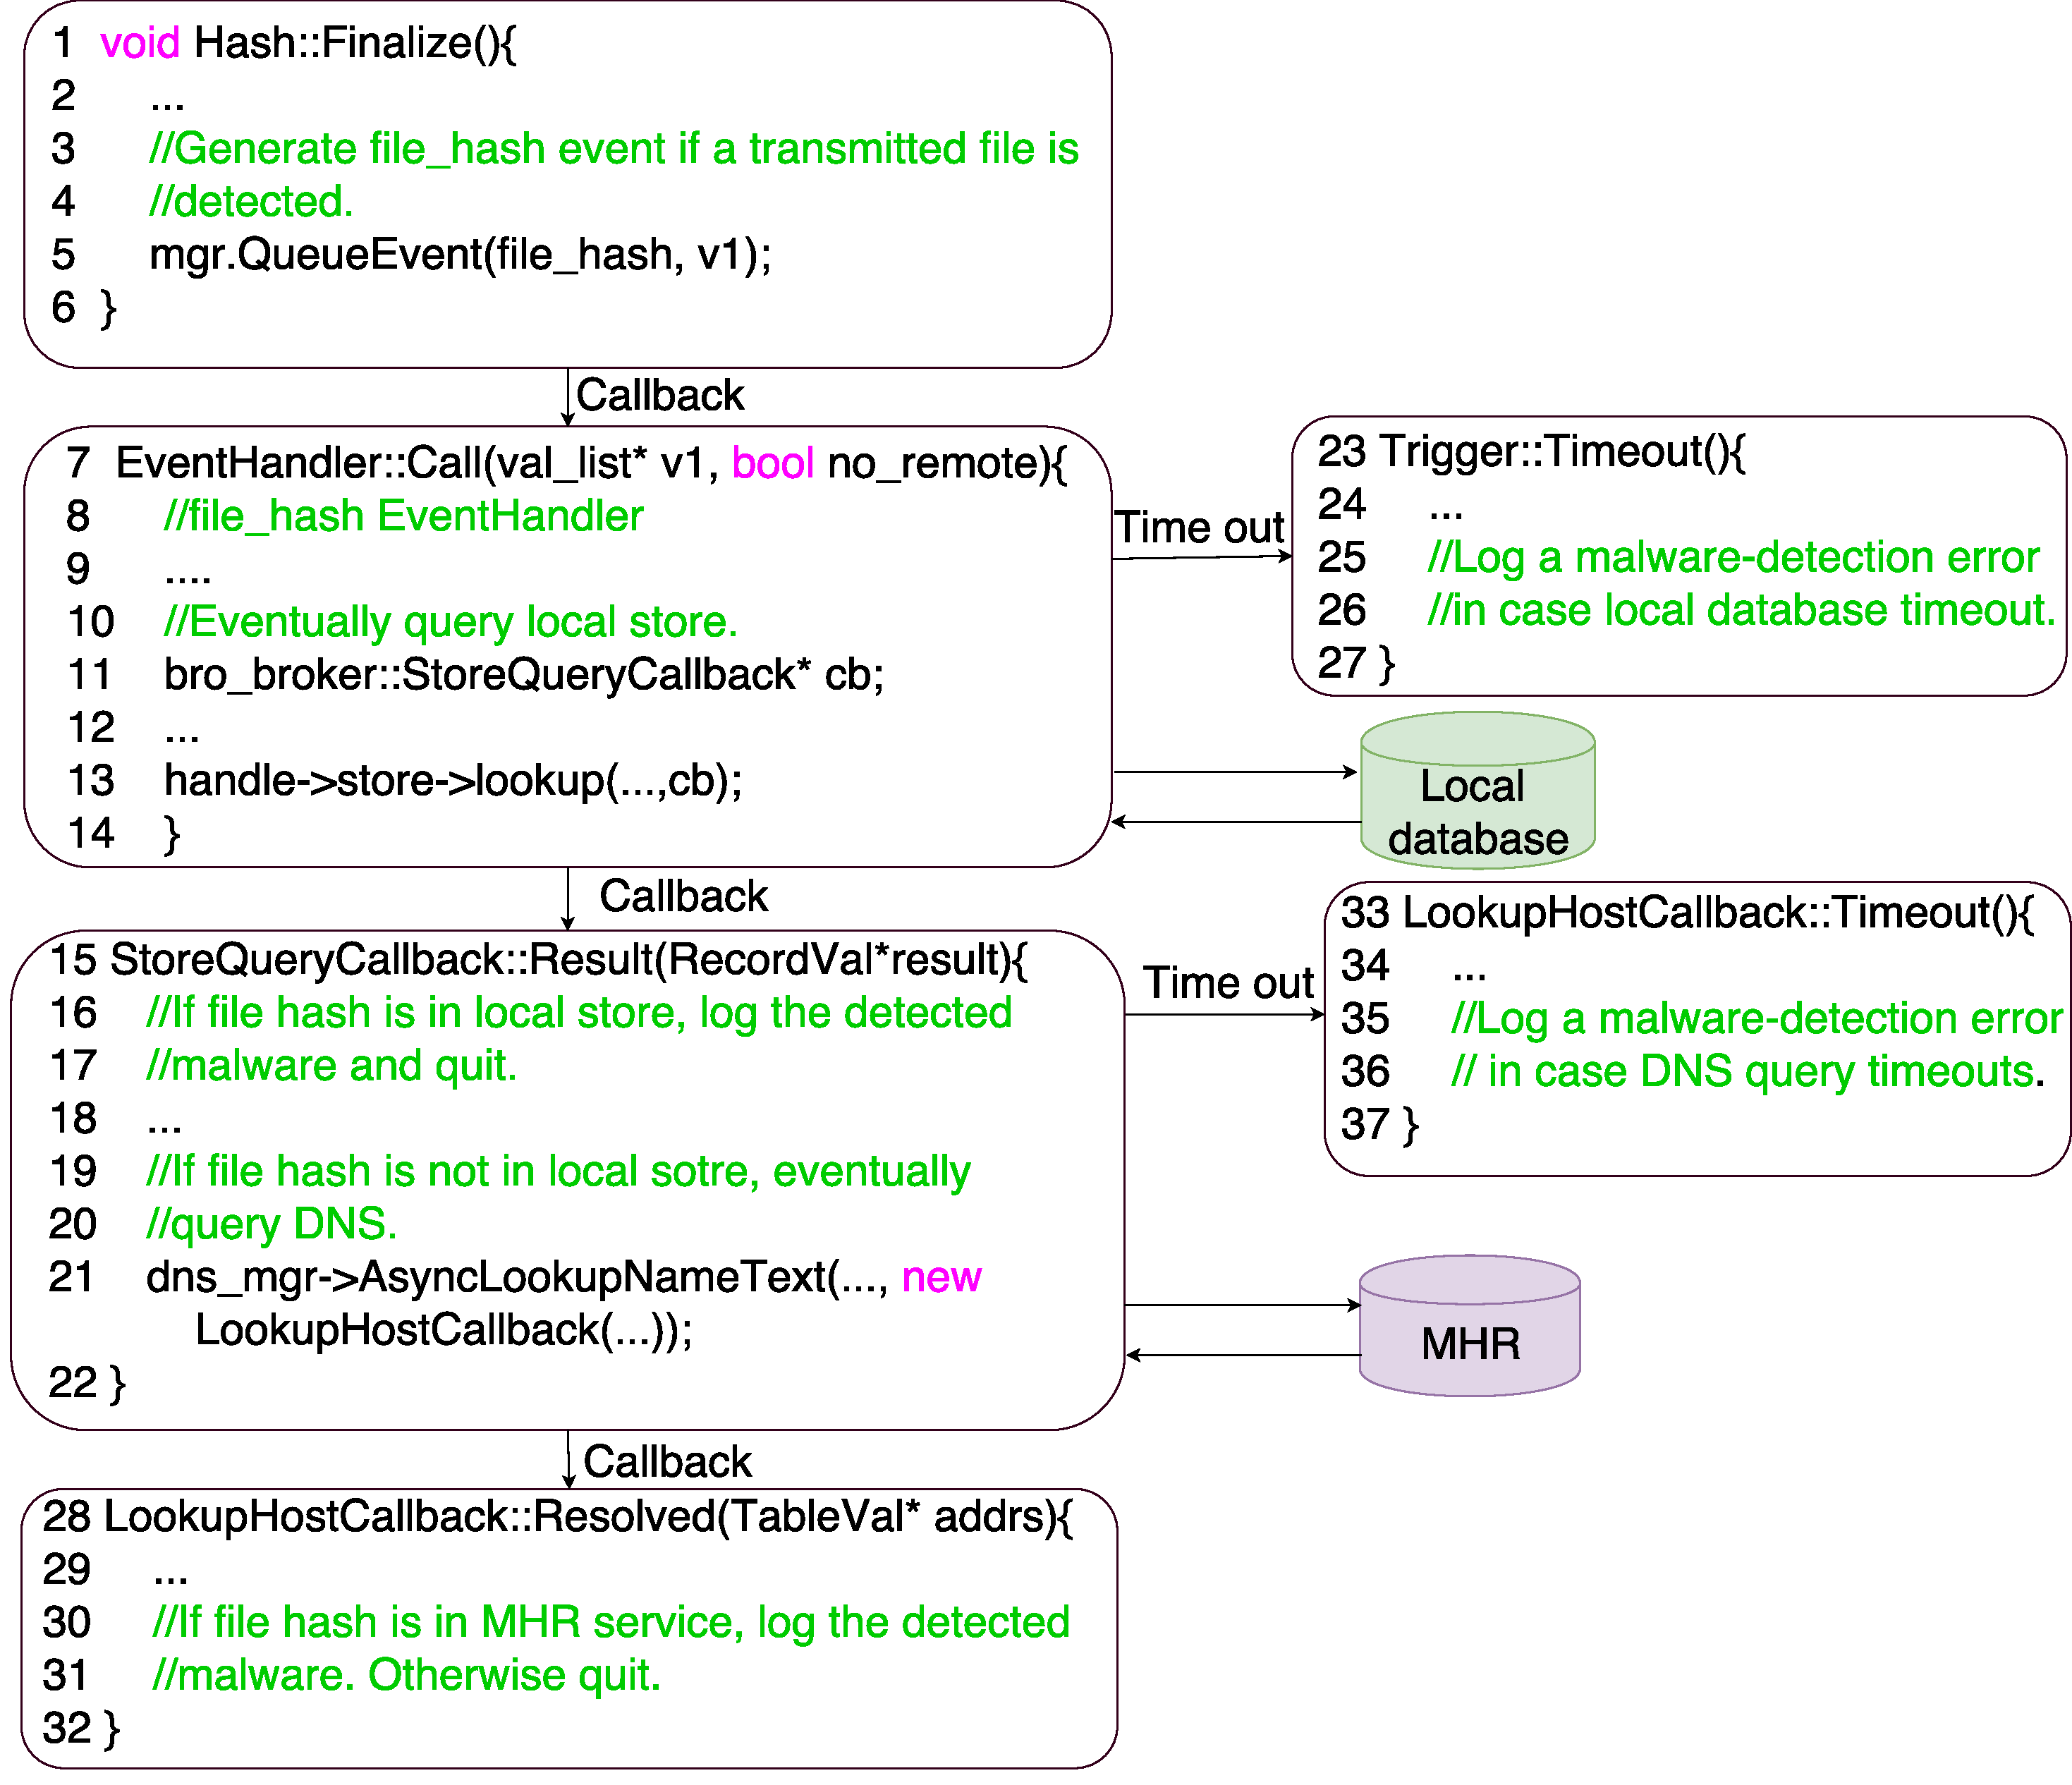
\includegraphics[width=\columnwidth]{chap-netstar/figure/ids_process_loop.pdf}
\caption{Malware detection in Bro.}
\label{fig:code-sample}
\end{figure}

\noindent\textbf{Bro.} We use a concrete example, malware detection in Bro IDS \cite{bro}, to demonstrate how asynchronous callbacks are used to program NFs. Bro can be configured to detect malware contained in a transmitted file as follows. % we can write a script to detect whether the transmitted file contains a malware. The detection method is to calculate a SHA1 hash over the content of the file and searching the calculated hash value over a set of pre-calculated malware hash values.
 A local database server %in Bro
 stores hash values of commonly-seen malware. For each TCP connection that goes through, Bro reconstructs its byte stream. % and analyzes the content of the byte stream.
 If a transmitted file is detected within the byte stream, Bro computes a SHA1 hash value over the file content, and queries the local database to obtain a quick response whether the hash value matches any malware's. In case of no hit in the local database, Bro can turn to the more complete and up-to-date Malware Hash Registry (MHR) \cite{MHR}, which provides a special DNS service: Bro can send a DNS request carrying the file hash to MHR, and the MHR responds whether there is a match with any of the malware hash values it has. If either of the two queries detects some malware, Bro raises an alarm in the log file.

The C++ code covering the execution path of the malware detection steps is given in Fig.~\ref{fig:code-sample}, as extracted from Bro version 2.5-359. In the packet processing loop of Bro, after a transmitted file is detected, \lstinline[style=InlineStyle]{Hash::Finalize()} is called to calculate the file's hash value and post a \lstinline[style=InlineStyle]{file_hash} event to Bro's event engine. Bro handles the event in the callback \lstinline[style=InlineStyle]{EventHandler::Call}, by performing an asynchronous query to the local database (lines 11,13). The response of the database query is handled by the callback \lstinline[style=InlineStyle]{StoreQueryCallback::Result}: if the file hash is not found in the local database, Bro performs another asynchronous query to the MHR (line 21). The DNS response is handled by a second callback, \lstinline[style=InlineStyle]{LookupHostCallback::Resolved}, which logs the detection of a piece of malware if the DNS response indicates so. %file hash is presented in MHR.
 Since any of the database and MHR queries may fail, two additional callbacks, \lstinline[style=InlineStyle]{Trigger::Timeout()} and \lstinline[style=InlineStyle]{LookupHostCallback::Timeout()}, are registered to handle the database and MHR query timeout error, respectively.

%The code in Fig.~\ref{fig:code-sample} is fully asynchronous and achieves good performance
The code excerpt highlights the following disadvantages in callback-based asynchronous programming:
(1) The asynchronous code is more complex to implement as compared to a synchronous program. For instance, if \lstinline[style=InlineStyle]{StoreQueryCallback::Result} is to be implemented in a synchronous fashion, the programmer can directly proceed to handle the DNS response or the timeout event after calling a blocking DNS query function, without the need for saving the context information (omitted from line 21) and defining two extra callback functions elsewhere (lines 28 and 33). %\chuan{correct the line numbers}.
(2) Omitted in line 21, saving and retrieving context information can be quite troublesome, as Bro relies on reference counting to keep allocated objects alive, and needs to correctly increase the reference counts of all the objects that it intends to keep within the context when registering a callback.
(3) Two error handling functions are defined to handle potential errors in the two asynchronous operations. The two functions in fact implement the same logic, \ie, to log a malware detection error to the database, which are quite redundant.



%It is error-prone and tedious for an ordinary programmer to handle these complexities and repetitive code. Bro resorts to a powerful script engine \cite{}, \eg, all the concrete implementation of the callbacks (lines 7, 15, 23, 28, 33 in Fig.~\ref{fig:code-sample}) is automatically generated by the script engine. However, it is even harder to implement this script engine, % than all these asynchronous callbacks and it
% highly customized for IDS tasks. % making it hard to adapt to general-purpose dataplane processing.

%\subsection{Asynchronous Programming in Other NFs}
%\label{sec:ap_in_nf}

\vspace{1mm}
\noindent\textbf{HAProxy.}
%Asynchronous programming with callbacks increases the implementation complexity of NFs. %Besides the example code discussed in Sec.~\ref{sec:bro},
 We have also inspected the asynchronous program in HAProxy \cite{haproxy}, a high-speed proxy due to its completely asynchronous design. HAProxy accepts incoming user TCP connections, relays received packet contents, such as HTTP requests, to several servers (\eg, for load-balancing or connecting an internal network to the public network), and then relays the responses received from the servers back to the client.
 In order to poll a socket file descriptor to retrieve the incoming data over the TCP connection, HAProxy invokes three nested callbacks, \lstinline[style=InlineStyle]{iocb} (for accessing the socket), \lstinline[style=InlineStyle]{recv} (for receiving data from the socket) and \lstinline[style=InlineStyle]{rcv_buf} (for putting received data into buffer). These three callbacks are registered multiple times in various source files, making it hard to trace the execution flow of HAProxy without a deep inspection of the files.

%\chuan{illustrate significance of the problem: how often do the complicated callbacks happen in many representative NFs' core code?}

%\vspace{1mm}
%\noindent\textbf{S-CSCF proxy.}
%Some NFs even abandon asynchronous programming due to the implementation difficulties. An representative example is an open-source, industrial-strength S-CSCF proxy \cite{} implemented by Clearwater Project \cite{}. S-CSCF proxy needs to query an ENUM service \cite{} when processing user traffic, which is a special DNS service for translating a telephone number into an URI record that can be reached over the Internet. In Clearwater Project \cite{}, querying ENUM is implemented as a synchronous procedure: the worker thread is blocked after sending out the ENUM query and unblocked when the response is received. While this simplifies implementation, it may become a potential performance bottleneck when ENUM service is heavily queried.


%above lead to the following observation: When doing asynchronous programming in NF, it is often hard to strike a balance between good runtime performance and the simplicity of implementation. So a natural question to ask is: is there a method to achieve such a balance? We believe that the key lies in bringing advanced programming abstractions to process dataplane network flows.

\subsection{Advanced Programming Abstractions}

There is a tradeoff between simplicity and performance when implementing a NF program: On one hand, synchronous programming is easier but incurs poor performance. On the other hand, asynchronous programming using callbacks achieves much better performance at the cost of implementation complexity. Similar tradeoffs have been identified when people build server programs, such as web \cite{tornado-web-server} and database servers\cite{rethinkdb}.
The solution in those domains has been to use advanced programming abstractions, including coroutine \cite{coroutine} and future/promise \cite{claessen1999poor, li2007combining, wtf, syme2011f}, to manage the complexity of asynchronous programming while achieving good performance.

%Coroutine \cite{} is a lightweight cooperative thread. On each physical thread, there can be multiple coroutines running concurrently. A coroutine runs as if it runs in its own thread and it switches its execution to other coroutines via explicit yielding. When a coroutine needs to perform a blocking task, it saves its stack information and notifies a scheduler. The scheduler picks another coroutine to run. Only when the blocking task finishes, the coroutine that initiating the task is resumed.

%tornado web server uses coroutine. search coroutine http server
% https://rethinkdb.com/blog/improving-a-large-c-project-with-coroutines/
% and hard
Coroutine is a user-space cooperative thread: a coroutine explicitly yields its execution to other coroutines when it waits for asynchronous operations to complete. The coroutine paradigm has found its success in building asynchronous web servers \cite{tornado-web-server} and databases \cite{rethinkdb}. %\chuan{why is corouting an advanced programming abstraction? it seems just some thread execution mechanism. clarify}

With coroutine, asynchronous NFs can be very easy to implement. The NF program can be directly written as a synchronous program, which runs as multiple coroutines (threads) to handle different flows. Whenever a coroutine needs to perform an asynchronous operation, it yields its execution to other coroutines after saving its thread context, and then waits to be resumed when the asynchronous response arrives in the future.

Typical coroutine switching time can be up to hundreds of nano seconds. A typical high-performance NF needs to process hundreds of thousands of flows concurrently and millions of packets per second. The coroutine switching time may significantly slow down NF processing, which we have verified with experiments (to be presented in Sec.~\ref{sec:eval6}). % against asynchronous NFs built with future/promise abstraction.

In search for a suitable advanced programming abstraction for significantly reducing implementation complexity of asynchronous NFs, we have identified that the future/promise paradigm can be more suitable. %, if it can be properly brought in for dataplane packet processing.



%We also explore the possibility of using coroutine for NF and build a simple framework that uses coroutine to handle flow packets. For each new flow, the framework creates a new coroutine and runs the packet processing loop inside the coroutine. Whenever the NF needs to wait for asynchronous events, the coroutine simply yields its control and the NF switches to process other flows using other coroutines. We directly utilize the coroutine module in Seastar.

% However, the performance of this framework (measured in terms of number of packets processed per second) is 4-5 times slower than the framework using future/promise . Even though coroutines are user-space light-weight threads and context switches between coroutines are faster than heavy-weight kernel threads, the measured context switch time among coroutines is around 352ns. Since a single NF may processes more than 10K concurrent flows, such a context switching time is considered harmful. What's more, when using coroutines, we have lost the ability of consolidated error handling provided by future/promise.

%Therefore, compared with future/promise, coroutine is not a good choice to improve asynchronous programming for NFs.

%\subsubsection{Future/Promise.}

\subsection{Future/Promise}
\label{sec:intro-future-promise}

The future/promise abstraction is a light-weight, elegant model for asynchronous programming. It simplifies asynchronous programming by mimicking synchronous programming, and reduces redundant error handling logic by propagating exceptions.


\subsubsection{Future}
A future object is of type \lstinline[style=InlineStyle]{future<T>} and contains a value of type \lstinline[style=InlineStyle]{T}. % (the interface abstractions in this section follows those in the Seastar library).
There are two states for each future object, available and unavailable. When in the available state, a future object either contains a concrete value of type \lstinline[style=InlineStyle]{T} that can be directly used, or an exception. In the unavailable state, a future object is associated with a promise object, and can be turned into available state with the help of the associated promise object.

\subsubsection{Promise}
A promise object is of type \lstinline[style=InlineStyle]{promise<T>}, and associated with an unavailable future object. When needed (\eg, when the response of a remote query arrives, or the response times out and an exception is generated), the programmer can set either a concrete value, or an exception, to the promise object with the \lstinline[style=InlineStyle]{promise::set_value} method. The value/exception is then automatically propagated to the associated future object and turns it into the available state.

\subsubsection{Continuation Function}
The future/promise abstraction works together with continuation functions to achieve asynchronous programming. A continuation function can be appended to a future object using the \lstinline[style=InlineStyle]{future::then} method. The following code shows a continuation function appended to the \lstinline[style=InlineStyle]{fur} future object.

\vspace{-1mm}
\begin{lstlisting}[style=InlineStyle]
future<T> fur=pr.get_future();
fur.then([captured_variables...](T t){
...
});
\end{lstlisting}
\vspace{-1mm}

\noindent Here, the continuation is presented as a C++ lambda function \cite{cpplambda}. \lstinline[style=InlineStyle]{captured_variables} is a list of variables passed to the continuation function, which it is free to use. For instance, \lstinline[style=InlineStyle]{captured_variables} may contain a pointer to another object and the continuation function can visit this object by following the pointer. %`\lstinline[style=InlineStyle]{...}' represents the function body.
 \lstinline[style=InlineStyle]{(T t)} represents the input arguments to the continuation function.

A continuation function can be considered as a special callback function. If the future object that it is appended to is available, the continuation function is immediately invoked; otherwise, it is invoked the moment when the future object becomes available. When a continuation function is called, the future object passes its concrete value as the argument \lstinline[style=InlineStyle]{T} into the continuation function. %Therefore, the input argument type (\lstinline[style=InlineStyle]{T}) of a continuation function must be the same as the value type of the future object (\lstinline[style=InlineStyle]{future<T> fur}) that it is appended to.

\subsubsection{Transforming Future Object}
\label{sec:tranform-future-object}

%Another property of the continuation function is its ability to transform a future object.
 If a continuation function is appended to a future object \lstinline[style=InlineStyle]{a} of type \lstinline[style=InlineStyle]{future<A>}, creates a future object \lstinline[style=InlineStyle]{b} of type \lstinline[style=InlineStyle]{future<B>} and returns it as a future object \lstinline[style=InlineStyle]{transformed} of type \lstinline[style=InlineStyle]{future<B>}, then we say the future object \lstinline[style=InlineStyle]{a} is transformed into future object \lstinline[style=InlineStyle]{transformed} of type \lstinline[style=InlineStyle]{future<B>}, and \lstinline[style=InlineStyle]{transformed} only becomes available when both \lstinline[style=InlineStyle]{a} and \lstinline[style=InlineStyle]{b} are available. %; otherwise, it remains unavailable.
When \lstinline[style=InlineStyle]{transformed} becomes available, it contains the exact value of \lstinline[style=InlineStyle]{b}. % which is directly acquired from \lstinline[style=InlineStyle]{b}.

Consider the following example for asynchronous database and DNS queries:

\vspace{-1mm}
\begin{lstlisting}[style=InlineStyle]
// Query database.
future<db_res> db_fur=_db.lookup(_hash);
future<dns_res> fur=db_fur.then([this](db_res res){
  // Do something with the database query response.
  ...
  // Query DNS.
  future<dns_res> dns_fur=_dns.lookup(domain_name);
  return dns_fur;
});
\end{lstlisting}
\vspace{-1mm}

\noindent We first issue an asynchronous database query \lstinline[style=InlineStyle]{db.lookup()} to acquire a future object \lstinline[style=InlineStyle]{db_fur}, which contains the query response when it returns. Then, we append a continuation function to \lstinline[style=InlineStyle]{db_fur}. Inside the continuation function, an asynchronous DNS query \lstinline[style=InlineStyle]{dns.lookup()} is issued and a future object \lstinline[style=InlineStyle]{dns_fur} is obtained, which contains the DNS response once it is received. When the continuation function is done, a future object \lstinline[style=InlineStyle]{fur} is obtained, %This transforms \lstinline[style=InlineStyle]{db_fur} into \lstinline[style=InlineStyle]{fur},
 which becomes available when both \lstinline[style=InlineStyle]{db_fur} and \lstinline[style=InlineStyle]{dns_fur} are available (\ie, when both the database response and DNS response are received), and contains the received DNS response once available (passed from \lstinline[style=InlineStyle]{dns_fur}).

The returned future object can be associated with another continuation function, which further returns anther future object. In this way, we are able to chain multiple continuation functions to carry out a series of asynchronous operations. It allows us %to use the future/promise approach
to mimic synchronous programming while achieving full execution asynchrony. In the above example, the database and DNS queries appear to be sequentially executed but are in fact asynchronously performed. % as in a synchronous program.
 Also, there is no need to define callbacks elsewhere: the continuation function for handling the database response is defined right in place (in the same file where the database query is issued), but is invoked only when the database response arrives and \lstinline[style=InlineStyle]{db_fur} becomes available.

% asynchronous operation defined inside the continuation function right in place.   In particular, the database query and the DNS query are sequentially defined in the code, the continuation function is immediately appended after \lstinline[style=InlineStyle]{db_fur} is generated  continuation function is immediately appendedThe code first queries the database, wait for database response. Then it queries the DNS and wait for the DNS response.

% Since continuation function executes an asynchronous DNS query and returns the future object \lstinline[style=InlineStyle]{dns_fur} containing the DNS response, \lstinline[style=InlineStyle]{fur} represents a transformed future object containing the DNS response. \lstinline[style=InlineStyle]{fur} only becomes available when both \lstinline[style=InlineStyle]{db_fur} and \lstinline[style=InlineStyle]{dns_fur} become available. When \lstinline[style=InlineStyle]{fur} becomes available, it contains the DNS response that is queried in the continuation function.

\subsubsection{Consolidated error handling.}
\label{sec:consolidated-error-handling}
In previous example, to catch database and DNS query exceptions, we can simply append another continuation function to the future object \lstinline[style=InlineStyle]{fur} as follows:

\vspace{-1mm}
\begin{lstlisting}[style=InlineStyle]
fur.then_wrapped([](future<dns_res> f){
  try{
    f.get();
  }
  catch(...){
    // catch whatever exceptions thrown
    // during database or DNS query
  }
});
\end{lstlisting}
\vspace{-1mm}

\noindent Here, \lstinline[style=InlineStyle]{fur} may contain an exception that is either generated by database query or DNS query. This is due to the capability of the future/promise abstraction to propagate exceptions and bypass uncalled continuation functions in the chain, and push the exception to the final returned future object. For example, if an exception occurs during database query, \lstinline[style=InlineStyle]{db_fur} will contain the exception, and then pass it to \lstinline[style=InlineStyle]{fur} without running the continuation functions it is associtaed with; if the database query is alright but DNS query raises an exception, \lstinline[style=InlineStyle]{dns_fur} contains the exception and passes it to \lstinline[style=InlineStyle]{fur}. Finally, the exception is passed to \lstinline[style=InlineStyle]{f} when the continuation function \lstinline[style=InlineStyle]{fur.then_wrapped([](future<dns_res> f)} is invoked, thrown by \lstinline[style=InlineStyle]{f.get}, and caught inside a try-catch pair \cite{cppexception}.

Leveraging this consolidated approach to handle various errors that may occur during a series of asynchronous operations, we can effectively reduce redundant error handling code when developing asynchronous programs.

%Asynchronous operations, including logging and database writing in the previous code example, may fail and throw exceptions. Future/promise abstraction can quickly propagate the generated exception and by-pass the rest of the continuations. For instance, in the previous example, should the logging fail and throw an exception, the continuation function for database writing will be by-passed and the exception will be filled in the final future object \lstinline[style=InlineStyle]{result}.

%Leveraging this property, future/promise abstraction can implement consolidated error handling using the follow code:

%\vspace{-1mm}
%\begin{lstlisting}[style=InlineStyle]
%result.then_wrapped([](future<response> fur){
%  try{
%    fur.get();
%  }
%  catch(...){
%    // catch whatever exceptions thrown from
%    // previously-chained continuation functions
%  }
%});
%\end{lstlisting}
%\vspace{-1mm}

%Using a single try-catch pair (the default mechanism for catching exceptions in C++ \cite{}), future/promise abstraction can handle all the errors happened during database reading, logging and database writing. This can greatly reduce the number of error handling code.

\subsection{Bring Future/Promise to Dataplane}


We use the open-source Seastar \cite{seastar} library as the base for implementing our future/promise NF programming model: (i) Seastar is one of the most mature C++-based future/promise libraries, and such C++ based implementation introduces minimum runtime overhead, which is critical for high-performance NFs; (ii) Seastar is integrated with DPDK and has a built-in user-space TCP/IP stack, rendering a feasible ground for building various NFs.

However, Seastar is originally designed for creating high-performance database servers \cite{scylladb}. %Though integrated with DPDK and has a user-space TCP/IP stack,
 It only exposes a socket-like interface for interacting with application-layer payload and has no interface for directly retrieving and sending raw network packets. Yet, an interface for manipulating raw network packets is crucial for implementing L4 NFs, such as firewall, NAT and IDS.

%On the other hand, even if such an interface is added to Seastar, without another properly designed interface to process network flows, we may completely lose the advantages bought by the future/promise abstraction, as discussed in Sec.~\ref{sec:intro-future-promise}. A trivial interface design may directly expose a regular packet handler function that is invoked for each received flow packets. However, this design falls back to callback-based asynchronous programming model and leaves no room for utilizing future objects and chaining continuation functions.


%we need to build another interface that can smoothly combine a regular packet processing loop and future/promise abstraction together, so that we can fully utilize the power of future/promise abstraction to ease the implementation of asynchronous NFs.

This leads to the design of \netstar, a future/promise paradigm for building various NFs. \netstar~is built on top of Seastar, and novelly designs and integrates two stacks to handle raw network packets and application-layer traffic in a coherent framework.
% The major technical contribution of NetStar is the integration of a novel interface called async-flow interface, which simulates a regular packet processing loop for each network flow. Within this loop, NF application can easily concatenate complex asynchronous operations using future/promise abstraction.

%Written completely in C++14, Seastar introduces minimum overhead for using future/promise, making it a good candidate for bringing future/promise to network dataplane. \chuan{add more introduction to seastar here, such that readers are clear why it is a good candidate for bringing future/promise to network dataplane.} However, this process is not trivial and we are facing the following challenges.

%Our primary challenge is that how to efficiently use future/promise model to process network flow packets. A naive implementation is to register a callback function that is invoked whenever new flow packets arrive \chuan{you can illustrate this point combining with figures to draw in the introduction section}. However, such a method falls back to traditional asynchronous programming model and loses all the power brought by future/promise. We have carefully designed a new operation model which we referred to as {\em asynchronous flow model}. Using this model, the NF can chain arbitrary asynchronous operations that mimics the control flow of a synchronous program when processing a single flow packet. The details of asynchronous flow model is further discussed in Sec.~\ref{sec:ai}.

%Our secondary challenge is to patch Seastar to expose interfaces for manipulating with raw packets.  While Seastar comes with a user-space TCP/IP stack based on DPDK, it only exposes POSIX-like interfaces for sending and receiving application-layer payload. We carefully introduce an native port module for manipulating with Seastar. The port module avoids unnecessary packet copy and offers fast and safe interfaces for manipulating with raw network packets.

%After solving these challenges, the end result is that we have a generic framework for building NFs that can address complex asynchronous programming in an efficient yet simple manner.

\section{The \netstar~Framework}
\label{sec:netstar-overview}
%Having realized about the advantages of \netstar, this section discusses the architecture of \netstar framework in detail. %is dedicated to a detailed introduction of the

\begin{figure}[!h]
  \centering
  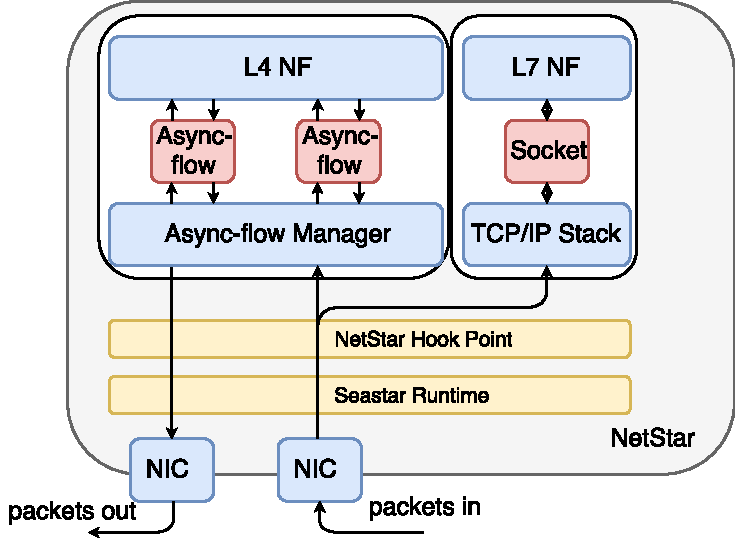
\includegraphics[width=0.6\columnwidth]{chap-netstar/figure/netstar-overvew.pdf}
  \caption{An Overview of \netstar.}
  \label{fig:overview}
\end{figure}

We design \netstar, a future/promise based programming framework for building various NFs that may carry out L4 or L7 packet processing tasks, and extensive asynchronous interactions with external services. For example, an IDS handles L4 packet processing by receiving TCP flows, reconstructing byte streams, and detecting whether they contain any malware. A proxy handles L7 application payload by forwarding application requests and responses between clients and servers. An overview of the \netstar~framework is given in Fig.~\ref{fig:overview}.


\netstar~is integrated with Seastar's runtime module, which uses DPDK to fetch packets from NIC queues directly into the user space.
\netstar~adopts a `dual-stack' design, including modules to handle packets in L4 and L7 application traffic. When \netstar~is used to implement an NF which handles L4 network packets (\ie, transport-layer packets), the hook point is configured to forward the packets received through the runtime to the async-flow manager. When \netstar~is used to implement an NF handling L7 application-level payload (\eg, a proxy), the hook point forwards the flows to the user-space TCP/IP stack. In an NF which involves both L4 and L7 traffic, the hook point classifies the packets according to their IP addresses, forwards packets whose IP addresses matches configured destination IPs to the TCP/IP stack, and others to the async-flow manager. For an IDS that carries out malware detection as in Sec.~\ref{sec:bro}, it handles L4 traffic (the TCP flows being inspected) and L7 traffic (database and MHR queries); packets carrying IP addresses of the database and MHR servers will be forwarded to the TCP/IP stack and the others to the async-flow manager.


%The TCP/IP stack of Seastar is pre-configured with an IP address. The hook point directs various L2-L4 packets that target this IP address, including ARP, ICMP TCP and UDP packets, to the Seastar TCP/IP stack for socket processing.



%\netstar is a framework  for building various NF applications that can handle various L2-L7 traffic and a variety of NFs including proxy, firewall, ids, and etc. At the lowest level, \netstar is integrated with DPDK for direct user-space packet accessing via NIC port. After packets enters \netstar, a customizable hook point classifies and dispatches packets to either (i) the user-space TCP/IP network stack or (ii) the async-flow manager, depending on the header information of the packets.

%\netstar re-use Seastar user-space TCP/IP stack to handle application-layer requests. The hook point directs TCP or UDP packets with a matching IP address to the TCP/IP stack by default. Seastar user-space TCP/IP stack exposes an interface that is similar to traditional POSIX socket. The NF application (i.e. HTTP reverse proxy \cite{}, NFs that require DNS query \cite{}) can uses the exposed socket to process application-later requests.


\textbf{Build an L4 NF.} To process L4 packets, a special interface, referred to as the {\em async-flow interface}, is designed, which consists of an async-flow manager and several async-flow objects. %After the hook point distributes matching packets to the manager,
The manager classifies received packets from the hook point into different network flows and pushes each flow to one async-flow object. The async-flow objects implement NF processing logic inside a simulated packet processing loop, using the future/promise abstraction for asynchronous operations. We will discuss our detailed design of the async-flow interface in Sec.~\ref{sec:netstar-framework}.

\textbf{Build an L7 NF.} To handle L7 application-level payload, we reuse Seastar's TCP/IP stack. The socket interface exposed by the TCP/IP stack is a modern re-implementation of the traditional POSIX socket based on the future/promise abstraction. An established TCP connection exposes a socket, through which an input stream for reading and an output stream for writing application data are available. % which facilitates asynchronous server programming for exchanging application level requests with the clients.

%\textbf{Other Usages of Seastar TCP/IP Stack.}
%Chuan: remove since it is not our contributions In \netstar, the TCP/IP stack can also be used by L2-L4 NFs built with the async-flow interface. In this way, various built-in features in the Seastar TCP/IP stack, including the DNS query interface and the RPC interface, can also be used by L2-L4 NFs. This greatly boosts the flexibility of our framework.

%\textbf{Thread Model.}
An NF built with \netstar~uses a share-nothing thread model. %, as provided by the Seastar runtime system.
Each NF runs multiple threads. Each thread is created and pined to one CPU core by the runtime. Each thread creates a complete set of modules, including the async-flow interface (one async-flow manager and multiple async-flow objects), the TCP/IP stack and the NF logic, and does not share these modules with any other thread. Incoming packets are distributed to different threads in a load balanced fashion, by configuring RSS \cite{rss} on the incoming NIC port. In this way, performance overhead associated with thread scheduling and shared resource contention is avoided. % and NFs built with \netstar~may achieve the best possible packet processing throughput.

\section{Async-flow Interface}
\label{sec:netstar-framework}

%This section gives a detailed introduction to the async-flow interface. The async-flow interface is divided into a manager, which distributes flow packets to different async-flows; and async-flow objects, which can be used for implementing NF logic that need complex asynchronous interactions.

Our major challenge when designing the async-flow interface is how to exploit the power of the future/promise abstraction while exposing easy-to-use interfaces for building NFs. We carefully design a simulated packet processing loop and use returned future objects to concatenate asynchronous operations, to address the challenge.

\subsection{Async-flow Manager}
\label{sec:async-flow-manager}

%The manager is responsible for distributing flow packets to different async-flow objects, creates new async-flow objects when new network flows arrive, and notifies the NF core processing logic the new async-flow objects. %It serves as an entry-point for various L2-L4 NF applications according to \lstinline[style=InlineStyle]{run_async_flow_manager} function defined in Fig.~\ref{fig:netstar-code-sample}.

After a packet is delivered to the async-flow manager from the hook point, the manager first retrieves flow information from the packet header to build a flow key. By default, the flow key is based on the flow 5 tuple (source/destination IP addresses, source/destination port and protocol type) of each TCP/UDP
packet. The manager uses the key to identify an async-flow object from a hash map: if a corresponding async-flow object is found, the received packet is sent to the async-flow object; otherwise, the packet belongs to a new flow, and the manager creates a new async-flow object for the key, and updates the hash map. %, and forwards the packet to the new object.
The manager also configures the new async-flow object % the manager directly reports it to the NF. The NF can then configure the new async-flow object
 with interested events (file hash event)
 %\chuan{add examples}
and core processing logic of the NF, using programming interfaces exposed by the async-flow object.



%Its basic usage has been demonstrated in the \lstinline[style=InlineStyle]{run_async_flow_manager} function in Fig.~\ref{fig:netstar-code-sample}.  has an expressive user interface as shown in Fig.~\ref{fig:netstar-code-sample}. The NF application defines what kind of NF should be created to handle the new async-flow object inside the continuation function, which is called when new flows arrive and new async-flows are created.


%Using the async-flow manager, the NF can acquire newly created async-flow object, register interested events exposed by this async-flow object and run the underlying NF processing logic for the underlying network flow.For a new flow, the manager further encompasses the new async-flow object and the new flow packet inside a context object, which is referred to as a new {\em flow context}. The new flow context is placed into a queue. The NF core processing logic is then notified to fetch the new flow context from the queue.

%For each new async-flow object, the manager first configures what events should be reported to the core NF processing logic from the preprocessor. Then the manager registers a packet handler function that implements the core NF processing logic to the async-flow object.


% configures the core NF processing logic by registering a packet handler function to the async-flow object. %implemented inside a registered packet handler function.
%and the core NF processing logic with xxx

%\chuan{I cannot understand how the notification is done based on the following descriptions and the future/promise introduction in Sec. 2. Revise carefully by specifying what is exactly the future object (value of the type) and continuation function (capture variables), what the continuation function does, and if any promise object is associated with the future object. Don't point to the example in Fig.~\ref{fig:netstar-code-sample}, but describe in general} The notification process is done via a special future object, which becomes available when the queue is not empty. This future object is returned to the NF application with \lstinline[style=InlineStyle]{on_new_async_flow} as shown in Fig.~\ref{fig:netstar-code-sample}. The NF application can append a continuation function to this future object like line 3 in Fig.~\ref{fig:netstar-code-sample}. This continuation function is only invoked when the queue that holds the new flow context is not empty, therefore the NF application can retrieve a new flow context within this continuation function and initiates the NF processing logic for this flow shown in line 4 to 9 in Fig.~\ref{fig:netstar-code-sample}. Eventually, when the new flow object obtained in the continuation function is destroyed, the first flow packet is delivered to the async-flow object.

%by calling \lstinline[style=InlineStyle]{cur_async_flow} as in Fig.~\ref{fig:netstar-code-sample}, construct an application-level object like \lstinline[style=InlineStyle]{malware_detector} as in Fig.~\ref{fig:netstar-code-sample}, register interested events for this application-level object to handle and eventually initiates the entire NF processing logic by registering a new loop function as shown in line 8 and 15 in Fig.~\ref{fig:netstar-code-sample}.

\subsection {Async-flow Object}
\label{sec:async-flow-object}

\begin{figure}[!h]
\centering
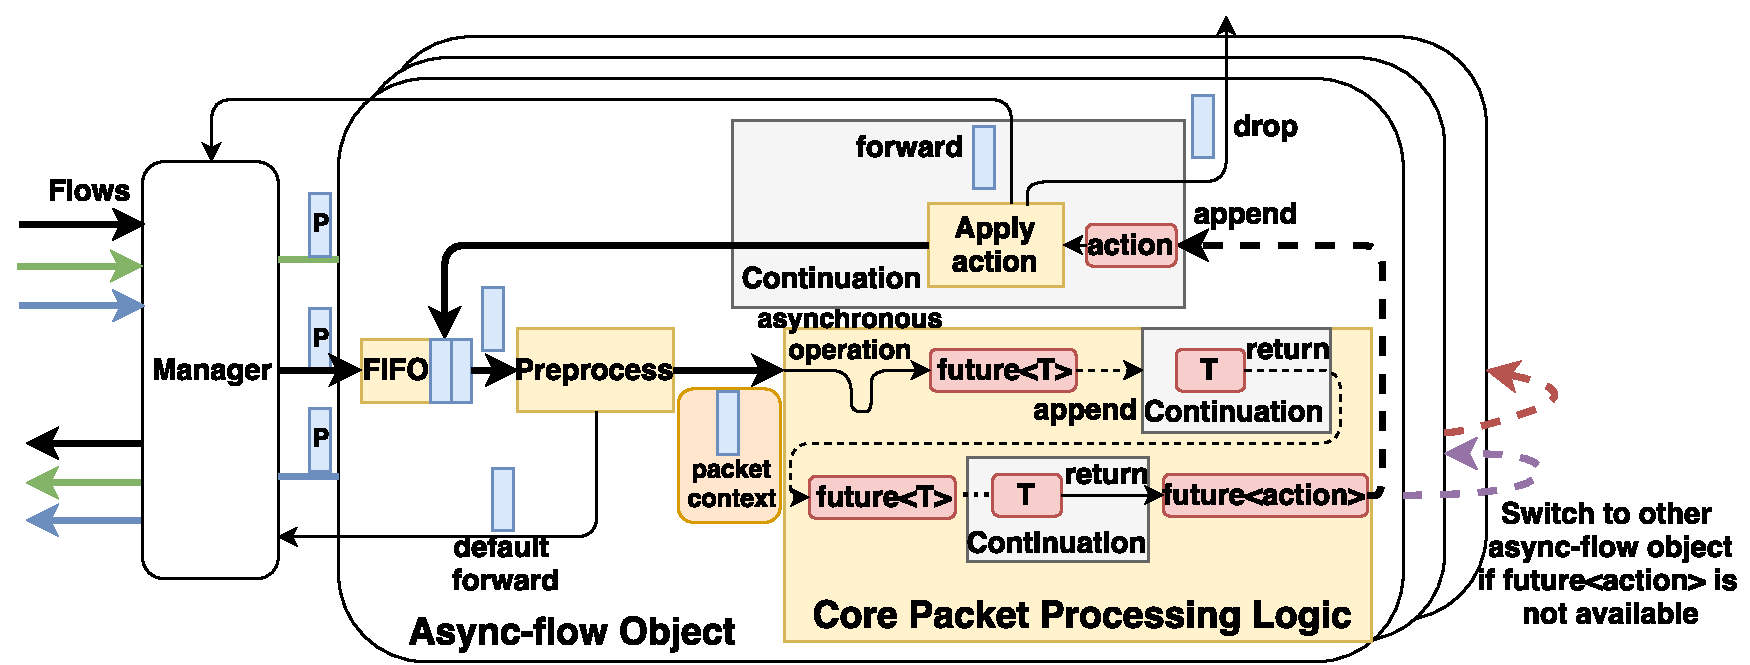
\includegraphics[width=\columnwidth]{chap-netstar/figure/async-flow-object.pdf}
\caption{Workflow of async-flow objects (P represents a packet).}
\label{fig:simulated_loop}
\end{figure}

The async-flow objects are key components to implement asynchronous packet processing in an NF. We target the following design objectives in its design.
(1) \textbf{Ease of Use.} The exposed programming interfaces should be easy to use, especially for programmers to implement NFs.
(2) \textbf{Full Processing Asynchrony.} %Asynchronous packet/flow processing should be fully supported.
After an async-flow object launches an asynchronous operation when processing a packet, it should yield its execution immediately to other async-flow objects, without blocking.

% To handle flow asynchronous, the async-flow object or the \netstar~framework should ...; to handle request asynchrony, ...
% In particular, when the NF application performs an asynchronous operation, the async-flow object should properly preserve the current processing context and the NetStar framework should switch to process other meaningful tasks. On the other hand, the exposed interface should be well integrated with future/promise abstraction to simplify asynchronous programming.

%For each new async-flow object, the manager first configures what events should be reported to the core NF processing logic from the preprocessor. Then the manager registers a packet handler function that implements the core NF processing logic to the async-flow object.

In \netstar, the programming interfaces exposed by the async-flow object to a programmer include an interface for registering a special packet handler function that implements the core NF processing logic, and an interface for configuring what events to be reported to the registered packet handler function. % from the preprocessor.
 The interfaces are easy to use: registration of a packet handler function %the function is regularly invoked by the async-flow object to process the received packet,
 is very much the same as implementing a packet handler in existing NF architectures~\cite{bro, snort}.

%xxx  We achieve design objective 1 above by ... exposing xxx that the NF programmer can register xxx with, such that the event ... and the core processing logic can be regularly invoked to process the received packet, in the same way of implementing a packet handler as in many existing NF architectures \cite{}.
%We can make async-flow object expose a loop function for the NF application to register. The loop function can then be regularly invoked to process the received packet, like a regular packet handler seen in many existing NF architectures \cite{}.

To achieve the second objective, we strategically simulate a packet processing loop within each async-flow object via a series of future-continuation chains, pause a packet processing loop if any intermediate future object is unavailable, and only resume it when the future object becomes available. %The simulated packet processing loop keeps running by recursively invoking the entry point of the simulated loop from a continuation function.
An illustration of the workflow within and among async-flow objects is presented in Fig.~\ref{fig:simulated_loop}.

%If the loop function is directly implemented as a regular packet handler function, then the loop function can only execute asynchronous operations via extensive use of callback functions, which complicates asynchronous programming.
% loop function returning a future object containing an action decision, and simulate a packet processing using the returned future object.

%\subsubsection{Simulated Packet Processing Loop} We discuss how the simulated packet processing loop work by tracing the execution of a flow packet as shown in Fig.~\ref{fig:simulated_loop}.
%In each async-flow object, we simulate a packet processing loop. %\chuan{explain why you say `simulate' or `simulated' packet loop, what are you simulating?}.
%After the packet is delivered to the async-flow object from the manager, the async-flow object checks whether the simulated packet processing loop is running. If so,

\vspace{1mm}
\noindent\textbf{FIFO Queue.} When a packet is sent from the manager to the async-flow object, the packet is first pushed into an FIFO queue and waits to be fetched by the packet processing loop. %Otherwise, async-flow object launches the simulated loop to process the packet.

\vspace{1mm}
\noindent\textbf{Preprocessing.} When a packet goes into the packet processing loop,  it is first preprocessed to generate a set of events. %This design is inspired by mOS \cite{}, as the arrival of a packet may trigger more interested events after preprocessing than the packet arrival itself.
 For instance, if an in-sequence TCP packet arrives, the preprocessing may retrieve new payload from the reordering buffer to reconstruct the TCP byte stream and report it as an new event, along with arrival event of the TCP packet. In this way, some functionalities within the core processing logic can be offloaded to the preprocessing step for simplification. \netstar~is equipped with four default preprocessors: a simple UDP preprocessor and a simple TCP preprocessor report packet arrival events; a TCP tracking preprocessor reports events on TCP packet arrival, TCP connection status change and the reconstruction of the TCP bytestream; a file extraction preprocessor extracts transmitted files from the byte stream and reports hash values of the files as events. All four preprocessors are equipped with a timer to report flow time-out events, when the async-flow object can gracefully shut down its packet processing loop.


After preprocessing, a packet {\em context} object is constructed, containing the current packet and all the generated events. If none of the events matches any of the events that the NF is interested in (\eg, an IDS may only be interested in reconstructed TCP byte stream, not the arrival of an out-of-order TCP packet), a default action is performed, \ie, forwarding the packet out (to the next-hop NF or the flow destination), and another packet is fetched for preprocessing from the FIFO queue; otherwise, the packet context is sent to the core processing logic for further processing.

%\subsubsection {Preprocessing and event extraction.}
%\label{sec:preprocessing-event-extract}


%\textcolor{blue}{The purpose of the preprocessing layer is to extract interested events, %(chuan: no need to mention) as inspired by mOS \cite{},
%including flow timeout events, packet arrival events, and other possible events that the NF application would like to tackle. Currently, the preprocessing later is implemented as a C++ template. NetStar provides three default preprocessors. A simple UDP preprocessor and a simple TCP preprocessor are used to report only packet arrival event and flow timeout event. A TCP tracking preprocessor is used to report events about TCP connection status change and reconstruction of the TCP bytestream.}


%\textit{First,} returning a future object from the loop function enables programmers to utilize future/promise abstraction. To concatenate an asynchronous operation, the programmer can initiate a asynchronous operation first, and then within the continuation function, returns the future object containing the action decision. According to the properties define in Sec.~\ref{}, the resulting future object still contains an action decision, but it will only become available when the asynchronous operation ends.




\vspace{1mm}
\noindent\textbf{Core Packet Processing Logic.}
In the core processing logic, events from the packet context are retrieved and packet processing logic is executed together with a number of asynchronous operations, carried out through a chain of future/promise objects and continuation functions. To handle one asynchronous operation, a future object is constructed, associated with a promise object, and a continuation function is appended to the future object. When the promise object turns the future object into available state (when the asynchronous operation is completed), the appended continuation function is invoked, which carries out corresponding processing based on the received response and returns another future object for handling the next asynchronous operation. Multiple asynchronous operations can be handled using such a `future/promise-continuation' chain.

%For instance, a firewall may check for the event of new packet arrival, retrieve the header of the packet and compare it against an access-control-list.

Using malware detection in IDS as an example, the core processing logic includes two asynchronous operations: querying the local database and querying the MHR. A future object is first constructed to receive query response from the local database, and the database response is obtained as the concrete type of value in the future object. A promise is associated to turn the future into available state when the response returns. The appended continuation function is invoked then, and returns another future object, which receives query response form the MHR. The second future object obtains the MHR response as its concrete type of value and passes it to an appended continuation function, which may raise an alert in case that the response indicates the detection of a malware.


\vspace{1mm}
\noindent\textbf{Final Future Object and Its Continuation Function.} The last continuation function in the asynchronous `future/promise-continuation' chain is forced to return a future object containing an action decision (\eg, drop or forward in the malware detection example). This future object becomes available when all asynchronous operations in the core processing logic have been completed. A continuation function is appended to this future object, which receives the action decision from the future object and carries out the action accordingly (\eg, drops the packet or forwards it to the next hop. The current packet context is then destroyed, and the packet processing loop moves on to fetch another packet from the FIFO queue (if it is not empty), and recursively restarts itself.


\vspace{1mm}
\noindent\textbf{Switching to Another Async-flow Object.} After an async-flow object has issued an asynchronous operation, the thread that the async-flow interface is running in moves on to handle another async-flow object, \ie, the packet processing loop in another async-flow object starts to fetch packets from its own FIFO queue and processes them. Different async-flow objects implement exactly the same logic in an NF. The programming style in implementing packet processing logic is very much like synchronous programming, while full asynchronous packet processing can be achieved. %All these attribute to our effective interface design based on the future/promise paradigm.
% we effectively utilize future object transformation provided by future/promise abstraction (see Sec.~\ref{sec:tranform-future-object}).




%\textbf{Return \lstinline[style=InlineStyle]{future<action>}.} By returning \lstinline[style=InlineStyle]{future<action>}, whether to forward or drop the packet is offloaded to the async-flow object. The async-flow object can append another continuation to the returned \lstinline[style=InlineStyle]{future<action>}: when \lstinline[style=InlineStyle]{future<action>} becomes available, then the loop function has finished all asynchronous processing and the async-flow is safe to forward or drop the packet depending the action decision contained in \lstinline[style=InlineStyle]{future<action>} and destroy the current packet context.

%\textbf{Run Simulated Loop Again.} During the execution of this simulated loop, new packets may arrive and get enqueued into the FIFO. To handle these packets, the simulated loop needs to be started again. This is also done in the continuation function appended to \lstinline[style=InlineStyle]{future<action>}: after applying packet forwarding decisions, if the FIFO is not empty, the async-flow object calls the entry function of the simulated loop again to restart the simulated loop.



%The second goal
%If the loop function is implemented as a regular packet handler, the loop function can only achieve this goal via extensive use of callback functions, which violates the principle of ease of use. Our solution is to let the loop function returns a future object containing an action decision about what to do with the currently processed packet. This solution is neat in several aspect:

%\textit{First,} returning a future object from the loop function enables programmers to utilize future/promise abstraction. To concatenate an asynchronous operation, the programmer can initiate a asynchronous operation first, and then within the continuation function, returns the future object containing the action decision. According to the properties define in Sec.~\ref{}, the resulting future object still contains an action decision, but it will only become available when the asynchronous operation ends.

%\textit{Second,} by returning an action decision, we offload the decision to forward or drop packet to the async-flow object. Therefore we can easily save all related context information, including the current packet and the exposed packet, within the async-flow object. To track this context information, we can simply saves a pointer to the container object like the malware\_detector object shown in Fig.~\ref{}.

%\textit{Third,} this allows us to simulate a packet processing loop. The async-flow object can append another continuation function to the future object returned from the loop function. Inside this continuation function, the async-flow object can recursively call loop function again to simulate a real loop function.


%A regular packet handler can only achieve this goal via extensive use of callback functions, which may

%For a regular packet handler function, it is hard to accomplish th

% Async-flow object exposes an iterative function which can be used by NF application to implement the core NF processing logic. The async-flow object also delivers various events, including flow time out and packet arrival event to the NF application. Most importantly, the design of the iterative function preserves the power of future/promise abstraction: the NF application can carry out arbitrary asynchronous operations inside the async-flow object with ease as illustrated in Fig.~\ref{fig:code-sample}.

%\subsubsection {Exposed Interface.} The async-flow object exposes two kinds interfaces for the NF applications.

%\textbf{An Iterative Function.} When a new async-flow object is created, NF application should register an iterative function to the async-flow object, which is called when interested new events happen. Inside the iterative function, the NF application can use the async-flow to query the current interested events and implement NF processing logic. The only restriction that NetStar impose on the iterative function is the type of its return value (via C++ compiler type checking). The iterative function must return a future objection containing an action result. When the future becomes ready, the async-flow knows how to perform post-processing about the current events.

%\textbf{Event Query.} The async-flow is equipped with a customizable preprocessing layer, which performs preprocessing to the received packet and generate an event for the iterative function to handle. The iterative function uses the event query interface exposed by async-flow to query and handle the event. This is inspired from the event system design of mOS \cite{}.

%\subsubsection {Simulated loop.} The async-flow achieves its functionality by running a simulated loop. By loop, we mean that the iterative function provided by the user will be sequentially invoked for each received flow packet. By simulated, we mean that we are not actually running a regular \lstinline[style=InlineStyle]{for} loop or \lstinline[style=InlineStyle]{while} loop in C++. If the async-flow runs a real loop, NetStar loses all the possible flow-level asynchrony, as multiple loops can not be scheduled within a single thread without using coroutine (see Sec.~\ref{}). In that case, only a single loop can run and consume all the thread execution time.

%The simulated loop is implemented by recursively calling the \lstinline[style=InlineStyle]{simulated_loop} function from a continuation function as shown in line 21 in Fig.~\ref{fig:simulated_loop}.

%Initially, the simulated loop is not launched and the async-flow waits for new packets. Once new packet is received, async-flow calls \lstinline[style=InlineStyle]{on_new_packet} function to launch the simulated loop (line 1). Since each async-flow object can only own a single simulated loop, we use a fifo queue to buffer the packet if the simulated loop is running and processing other flow packets (line 2). The simulated loop is restarted again if it not running when async-flow receives a new packet (line 5-6).

%After the packet is preprocessed and the event context is constructed (line 11-14), the iterative function is called for processing the event. Remember that the iterative function returns a future object containing an action result. We immediately chain a continuation function to this future object, which calls recursively calls the \lstinline[style=InlineStyle]{simulated_loop} function.

%Before the future object returned by the iterative function becomes ready, all the newly received packets will be pushed back into the fifo queue. Therefore the iterative function is free to carry out any kind of asynchronous operations. When the iterative function blocks and waits for an event to happen, the NetStar framework simply switches to other meaningful. Eventually, when the future object becomes available, \lstinline[style=InlineStyle]{simulated_loop} is called again to process other packets received when the async-flow is blocked.

%In Seastar, the continuation function is an heap-allocated function object and pushed to an execution queue for invocation, therefore recursively call a function within the continuation function will not cause errors like stack overflow.

\subsection{Asynchronous Programming With \netstar: the IDS Example}
\label{IDSexample}

\begin{comment}
\begin{figure}[!t]
\centering
\begin{lstlisting}[style=CStyle]
void run_async_flow_manager() {
  repeat([this]{
    return _manager.on_new_async_flow().then([this]() {
      auto af = _manager.cur_async_flow();
      do_with(malware_detector(std::move(af)),
        [](malware_detector& nf){
          nf.events_registration();
          return nf.run();
        });
      return stop_iteration::no;
    });
  });
}
future<> malware_detector::run() {
  return _af.register_loop_fn([this](){
    ...
    if(_af.preprocessor.on_file_hash_event()) {
      // Get file hash from preprocessor.
      auto _hash=_af.preprocessor.get_file_hash();
      return _db.lookup(_hash).then([this](db_res res){
        if(malware_detected_in_db(res)){
          // File hash is stored in local database.
          record_detected_malware();
          return ready_future(action::drop);
        }
        // File hash is not stored in local database.
        string name=build_up_name(_hash);
        return _dns.query(name).then([this](dns_res res){
            if(malware_detected_in_mhr(res)){
              // File hash is presented in MHR.
              record_detected_malware();
              return ready_future(action::drop);
            }
            // File passes malware detection.
            return ready_future(action::forward);
        });
      }).then_wrapped([this](future<action> f){
        try {
          return f.get();
        }
        catch(...) {
          // Either database or DNS query timeouts.
          record_malware_detection_error();
          return ready_future(action::drop);
        }
      });
    }
    ...
  });
}
\end{lstlisting}
\caption{Malware detector implemented using \netstar.} %It uses the same detection method as in Bro.}
\label{fig:netstar-code-sample}
\end{figure}
\end{comment}


\begin{figure}[!h]
\centering
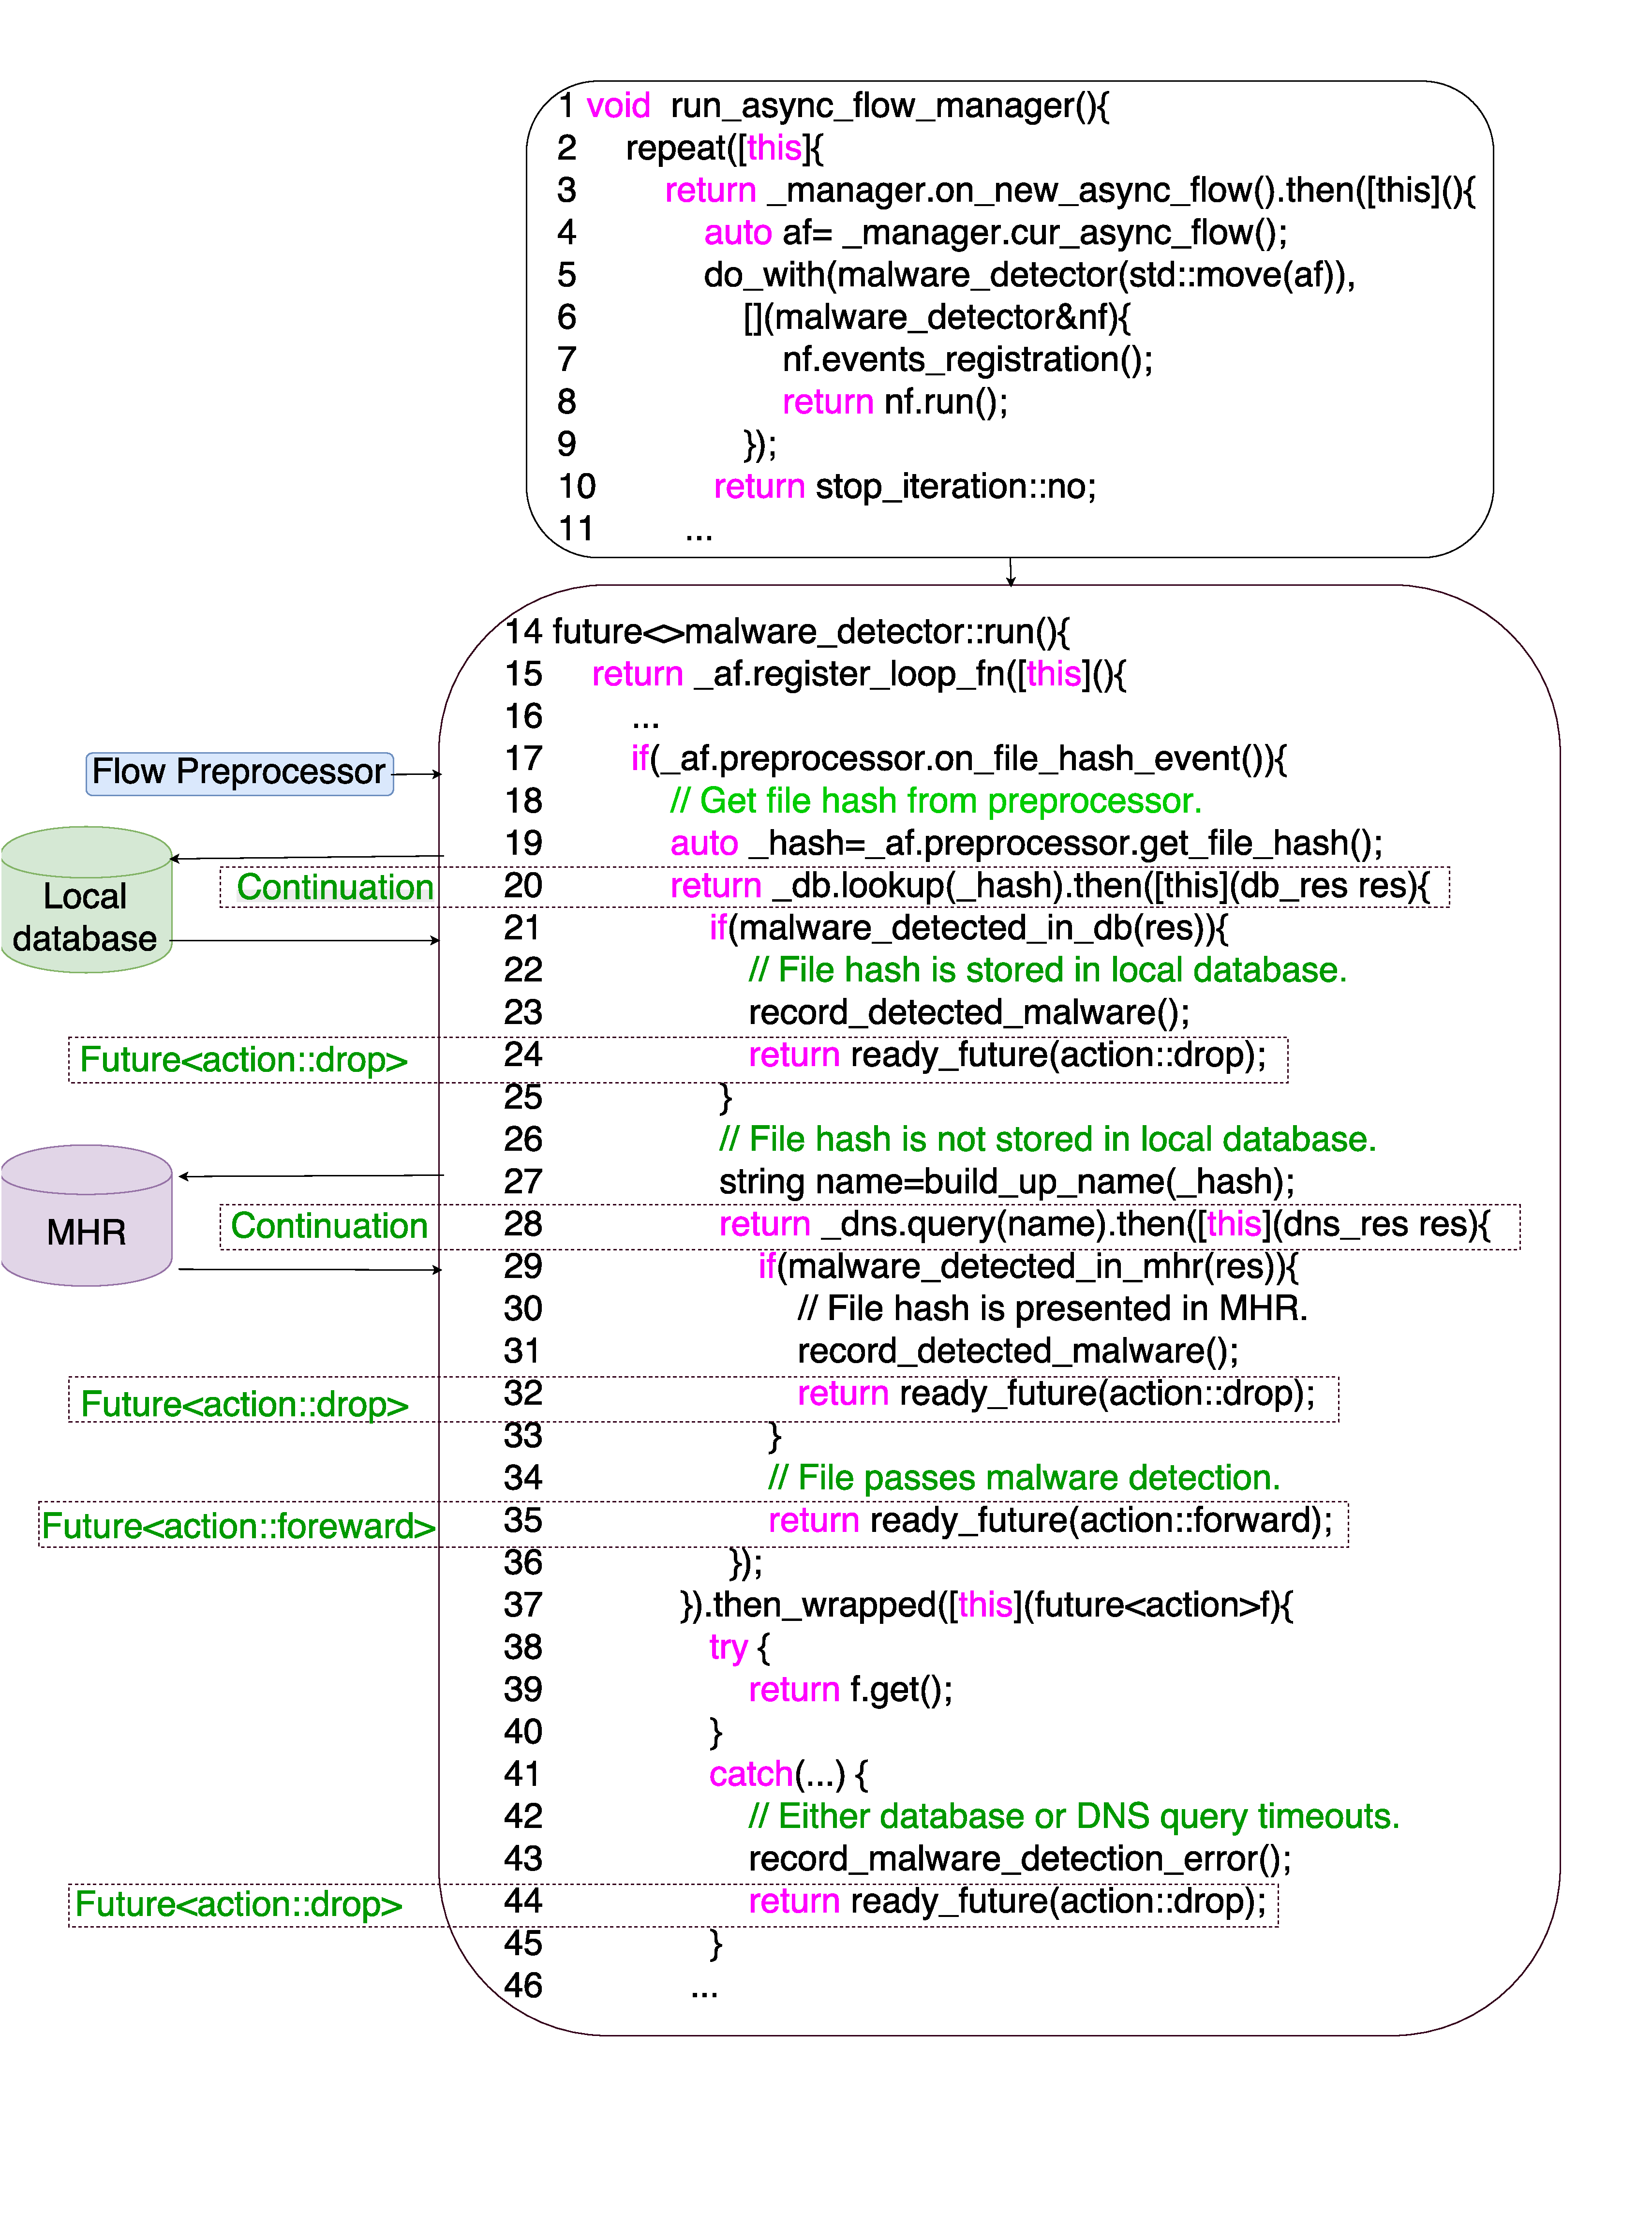
\includegraphics[width=\columnwidth]{chap-netstar/figure/netstar_code_graph.pdf}
\caption{Malware detector using \netstar.}
\label{fig:netstar-code-sample}
\end{figure}


Now we present the implementation of a malware detector using the async-flow interface designed above, which achieves similar functionalities as the Bro example in Sec.~\ref{sec:bro}. %, except the following: In Bro's implementation, when some malware is detected, only the event is logged %, and the packets are still forwarded to the next hop
%(mainly due to their implementation choice of decoupling the malware detection process from the packet processing loop); our code works in an in-line mode, that when it detects some malware in a flow, it drops all the subsequent flow packets and stops the flow from reaching the next hop.

Our code sketch is given in Fig.~\ref{fig:netstar-code-sample}. \lstinline[style=InlineStyle]{run_async_flow_manager} runs the async-flow manager, which constantly checks (lines 2-3) incoming new flows. If a new TCP flow has arrived, %(indicated by a new flow 5 tuple in a received packet),
a new async-flow object is created to handle the flow (line 4), and a malware detector object is associated with the new async-flow object (line 5). The malware detector object expresses its interest in the file hash event by registering this event %to the async-flow object
(line 7). The core processing logic of the malware detector is then registered with the async-flow object by calling \lstinline[style=InlineStyle]{register_loop_fn} (line 15),
%The malware detector is then started by calling \lstinline[style=InlineStyle]{run} (line 8). \chuan{explain what happens to existing flows. I do not see where in the code handling of existing flow is done}.
%In \lstinline[style=InlineStyle]{run}, core processing logic of the malware detector is registered with ...\chuan{registered with the async-flow object? change the name of loop in the code} (line 15), % does nothing but to register a loop function as in line 17,
which is carried out upon occurrence of the file hash event.


First, the preprocessor %to handle each received packet in the flow is a TCP payload reassembler, which
reconstructs the TCP byte stream as it receives each new flow packet (code omitted from Fig.~\ref{fig:netstar-code-sample}). After processing a packet, if the preprocessor detects a newly transmitted file, it calculates the hash value of this file and raises a the file hash event. % as discussed in Sec.~\ref{sec:bro}.
In case that the preprocessor fails to detect a transmitted file, it only raises a packet arrival event, which is ignored by the core processing logic, % registered by the malware detector object,
 and the packet is forwarded out directly.

After a file hash event is generated (line 17), the core processing logic %is called to handle this event
(lines 19-37) implements similar malware detection steps as discussed in Sec.~\ref{sec:bro}.
A database query is initiated by \lstinline[style=InlineStyle]{_db.loopkup} and a future object is obtained which contains the database response (line 20); a continuation function is appended for checking the query result. If some malware is detected, the packet is immediately dropped by returning a future object containing a drop action (line 24). Otherwise, it moves on to query the MHR with a DNS query using \lstinline[style=InlineStyle]{_dns.query} (line 28). The continuation function appended to the future containing the DNS query response checks the query result. If some malware is detected, the continuation function returns a future object containing a drop action as well (line 32); otherwise, the continuation function returns a future object containing a forward action (line 35). The code from line 38 to line 47 handles potential exceptions generated during database or DNS queries, as a continuation function appended to the returned future object.

%If a malware is detected, the malware detector records this detection by calling \lstinline[style=InlineStyle]{record_detected_malware()} (line 23 and 31). The \lstinline[style=InlineStyle]{record_detected_malware()} function asks the async-flow object to deliver all the packet arrival event to the malware detector object, which drops all subsequent packets by default.


\noindent\textbf{Comparison.} The malware detector implemented with \netstar~has the following advantages over that in Fig.~\ref{fig:code-sample}.
(1) {\em Simplified Implementation.} The malware detection process can be concisely implemented in \netstar~using only 18 lines of code (lines 19-37). Our code mimics the sequential execution of database and DNS queries within a single function, instead of spreading the execution flow across multiple functions.
(2) {\em Simplified Context Management.} In our code, the context information is put directly into the malware detection object. Different continuation functions (lines 15, 20, 28, 37) can easily visit the saved context by capturing a pointer (\lstinline[style=InlineStyle]{this}) to the malware detection object. Since the malware detector object is only destroyed when the packet processing loop stops running (line 5), the above code guarantees that the malware detector object is always alive when the continuation functions are being called.
(3) {\em Consolidated Error Handling.} Instead of defining two error handling functions, our implementation consolidates the error handling logic within a single continuation function (lines 38-47). %, eliminating redundant definitions.
The programmer can be more focused on the core NF processing logic, while simply chaining another continuation function at the end for handling all errors that might be generated from the core code.

%\chuan{`this' represents the packet context?}
%we capture a pointer to the malware detection object (\lstinline[style=InlineStyle]{this} shown in Fig.~\ref{fig:netstar-code-sample}) within different continuation functions (line 15, 20, 28, 37)
%. By putting all relevant context information within the malware detection object, NetStar simplifies context management
%The design of the async-flow interface uses reference counting \chuan{I do not see reference counting mentioned in  async-flow interface} to guarantee that when the continuation function is called, the malware detection object is never destroyed \chuan{clarify how is the related to context management}.

%{\em Support of Inline Mode.} The Bro code in Fig.~\ref{fig:code-sample} does not run in in-line mode. The malware detection process is decoupled from the packet processing loop of Bro. So that when the malware is detected, Bro can only log the event, instead of stopping the flow from reaching the target. Our async-flow interface design guarantees that while an asynchronous operation is going on, the packet can be buffered without releasing. When the asynchronous operation finishes, the async-flow interface determines whether to forward the packet or now by checking the value returned in the future object (line 24,32,35,44). In this way, we can effectively implement a malware detector that runs in inline mode to better protect the backend.

\section{Implemented NFs}
\label{implementation}

%The reason that we choose to implement \netstar on top of Seastar is two folds. First, Seastar has one of the most mature C++ future/promise implementation that allows future to be chained with arbitrary number of continuation functions. Other C++ future/promise implementations do exist \cite{}, but some of these are not mature enough to support chaining continuation functions. Second, Seastar has good integration with DPDK packet processing framework. In particular, it provides an efficient user-space TCP/IP stack and it is directly used by \netstar to implement application-level NFs like HTTP reverse proxy.

\subsection{Enhancing Seastar}

\netstar~is implemented on top of the Seastar framework, to exploit its C++-based future/promise implementation and DPDK support.
 %The Seastar framework is designed for server programs and not to manipulate raw L2-L4 network packets.
 Besides enabling raw L2-L4 packet processing that Seastar does not support, \netstar~makes several improvements.

 \noindent\textbf{Eliminating Packet Copy.} In its TCP/IP stack, Seastar does not use DPDK's RTE packet buffer \cite{dpdk}. Instead, it defines its own packet object and introduces two additional packet copies for copying the payload content of each RTE packet buffer to and from a packet object %The first copy is when Seastar polls a batch of RTE packet buffers, it copies the payload content of each RTE packet buffer to a newly constructed packet object. The second copy is when Seastar sends the packet object out, Seastar needs to copy the content of the packet object back to the RTE packet buffer. Seastar does provide a hack to eliminate the packet copy, but our test result reveals that it does not improve the overall system performance.
  While the additional packet copy does not affect the performance of the TCP/IP stack for building L7 applications, it does pose additional overhead for L2-L4 NFs. To eliminate the packet copy and speed up packet processing, we directly use RTE packet buffer for L2-L4 NFs. %, and only translate the RTE packet buffer to Seastar packet object whenever needed.
 %(chuan: add this to sec.3) We also implement a hookpoint that serves as a packet distributor as discussed in Sec.~\ref{framework}, so that we can run NF application and TCP/IP stack simultaneously for advanced functionalities like DNS query when processing raw network packets.

   %directly use RTE packet buffer for L2-L4 NFs.

  %, and only translate the RTE packet buffer to Seastar packet object whenever needed.
%(chuan: add this to sec.3) We also implement a hookpoint that serves as a packet distributor as discussed in Sec.~\ref{framework}, so that we can run NF application and TCP/IP stack simultaneously for advanced functionalities like DNS query when processing raw network packets.

\noindent\textbf{Multiple TCP/IP Stacks.} Seastar treats its TCP/IP stack as a singleton. But an NF program may need more than one TCP/IP stack if the NF, \eg, proxy \cite{haproxy}, handles more than one NIC port.
%\chuan{add an example}.
We improve Seastar to allow the creation of multiple TCP/IP stacks.

\subsection{Implementing Representative NFs}
\label{NFs}

We have built multiple representative NFs using \netstar.

\noindent\textbf{NFs from the StatelessNF paper \cite{201545}.} We reimplement four NFs from the StatelessNF paper, \ie, firewall, NAT, IDS and load balancer. Our implementation follows the pseudo-code logic in the paper, and leverages our async-flow interface. The major differences are: (1) we do not need to set up a dedicated polling thread for each worker thread to poll each NIC queue; each thread in \netstar~performs all the tasks including port polling and packet processing. %, while ensuring full asynchrony with low overhead.
(2) %Since \netstar~is fast has good scalability,
We use a fast in-memory key-value store, mica \cite{179747}, which has a larger throughput than the RAMCloud database \cite{ousterhout2015ramcloud} used in StatelessNF. %We also implement a custom client library for our NFs to read from and write to mica database. %\chuan{clarify whether this client interface is the same or different from the async-flow interface}.
(3) In StatelessNF, a unique thread is dedicated to contact RAMCloud for storing the per-flow states; with \netstar, the async-flow objects running in each thread can use the thread-local mica client library to contact mica server concurrently.
%\netstar~is equipped with a client interface that is created on each client thread \chuan{clarify what each client thread is and what the client interface is}. Since mica is partitioned and different client threads can concurrently read and write to mica,

\noindent\textbf{An HTTP reverse proxy.} We use the TCP/IP stack in \netstar~to implement an HTTP reverse proxy, whose functionality is similar to HAProxy (see Sec.~\ref{sec:bro}) and TinyProxy \cite{}: %, acting as a middleman between HTTP clients and servers:
it intercepts incoming TCP connections from clients, and relays HTTP requests to servers; it then receives HTTP responses from the servers and pushes them back to the clients. %Our proxy implementation leverages the enhancement for creating multiple TCP/IP stacks that we made to Seastar.

\noindent\textbf{An IDS that inspects HTTP payload.} This IDS detects potential intrusion from the reconstructed HTTP request payload using our async-flow interface, which is more complicated than the IDS implemented following the StatelessNF. %This IDS is equipped with a preprocessor for reconstructing the TCP byte stream. The core processing logic of the IDS parses converts the reconstructed TCP byte stream into a special input stream, which is fed to the built-in HTTP request parser of Seastar for checking whether the received byte stream contains a valid HTTP request. Once an HTTP request is received, the IDS passes the entire HTTP request payload to the AC automaton \cite{} to detect intrusion. The IDS drops subsequent flow packets if an intrusion is detected, otherwise forwards the packet.

% To compare the performance of this IDS, we re-implement a similar IDS with mOS library \cite{}. We choose mOS because it is the state-of-art library implemented with callback-based event-driven style. We can use an implementation in mOS to evaluate whether NetStar approaches state-of-art performance.

%When the HTTP reregisters reconstructed TCP byte stream  parses the TCP connection states and uses a reordering buffer to reconstruct the TCP bytestream. It parses the bytestream to extract HTTP requests and checks the HTTP request against a malware detection engine.

\noindent\textbf{A Malware Detector} as introduced in Sec.~\ref{IDSexample}. %The malware detector is equipped with a preprocessor for generating file hash event on transmitted files over reconstructed TCP byte stream. The core processing logic of the malware detector is implemented according to Fig.~\ref{}.
 It utilizes the async-flow interface and the TCP/IP stack in \netstar~concurrently. %In particular, we uses the TCP/IP stack to implement a database query interface. For DNS query interface, we re-use existing DNS module in Seastar. We also set up a database server and a DNS server in our cluster for the malware detector to query.

\section {Evaluation} \label{sec:netstar-evaluation}

In this section, we evaluate the performance of the various NFs built with \netstar. Even though future/promise paradigm can simplify asynchronous programming, using this paradigm adds additional overhead to dynamically create special runtime objects (Sec.~\ref{sec:intro-future-promise}). Therefore a natural question to ask is whether the performance of \netstar~is good enough to approach line-rate processing. To answer this question, we design a series of experiments to evaluate the maximum throughput achieved by the \netstar~NFs. We also compare \netstar~with several NFs that are implemented with fast, low-overhead callback-based method to reveal the overhead associated with using future/promise abstraction. The second question involves the effectiveness of future/promise abstraction for simplifying the implementation. To answer this question, we adopt a similar quantitative methodology \cite{syme2011f} used for evaluating F\# future/promise abstraction and compare the required lines of code for implementing the core processing logic between \netstar~NFs and NFs built with callback method.
% for implementing NFs using \netstar and

\subsection {Methodology}

\noindent \textbf{Testbed.} Our testbed consists of 5 servers: three Dell R430 servers, each equipped with one Intel Xeon E5-2650 CPU 2.30GHz with 10 physical cores and 48GB memory, and two Supermicro servers, each with one Intel Xeon E5-1620 CPU 3.50GHz with 4 physical cores and 32GB memory. All servers are equipped with two Intel X710 10Gbps NICs and they are connected through a Dell 10Gbps Ethernet switch. We divide the servers to run our NFs and traffic generators (flow sources and destinations). %Throughout our evaluation, we use one of the Dell R430 server to run our NF application. The rest of the servers are dedicated to traffic generation.

\noindent \textbf{Traffic generation.} We use two types of traffic generators. The first is a custom packet generator that we built on top of \netstar, which can generate 64-bytes UDP/TCP packets at 14Mpps (packets per second), \ie, 10Gbps. The number of flows and the packet size for generation are adjustable. This generator is used to produce flows to NFs such as the packet forwarder (Sec.~\ref{sec:eval1} and Sec.~\ref{sec:eval6}) and the NFs from StatelessNF paper (Sec.~\ref{sec:eval2}). To measure packet processing latency, this generator tags each produced packet with a generation time and computes the packet processing latency by an NF after receiving the packet back from the NF (in this case, source and destination of the flows are the same). The second traffic generator is the default HTTP benchmarking tool provided by Seastar. The tool runs in a client-server setting by sending a large number of HTTP requests from a client and receiving corresponding HTTP responses at the server. We modified this tool, including adding support for HTTP POST method for a client to upload files to the server and recording the HTTP transaction completion time, which is the time interval between sending HTTP request and receiving HTTP response. We use flows produced by this traffic generator to evaluate NFs such as the HTTP reverse proxy (Sec.~\ref{sec:eval3}), the IDS (Sec.~\ref{sec:eval4}) and the malware detector (Sec.~\ref{sec:eval5}).
%eval1 microbench, eval2 stateless nf, eval3 proxy, eval4 ids, eval5 malwares
% eval6 coroutine


\noindent \textbf{Metric.}
We focus on three types of key performance metrics. (1) \textbf{Packet processing throughput} achieved by an NF, measured in the number of processed packets per second (Sec.~\ref{sec:eval1},~\ref{sec:eval2},~\ref{sec:eval6}), the number of processed HTTP requests per second (Sec.~\ref{sec:eval3}) and total bandwidth consumed by all the HTTP connections (Sec.~\ref{sec:eval4}, ~\ref{sec:eval5}).
(2) \textbf{Latency}, computed as average packet processing delay (Sec.~\ref{sec:eval2}) or the average HTTP transaction completion time (Sec.~\ref{sec:eval3},~\ref{sec:eval4},~\ref{sec:eval5}). (3) \textbf{Lines of code (LOC)} for implementing the core packet processing logic, meant for comparing the implementation difficulty using our future/promise based framework and the callback-based asynchronous programming. %(following the approach used in \cite{syme2011f} which uses LOC as the metric to evaluate some future/promise implementation in C\#).

\noindent \textbf{Baselines.} For comparison with NFs implemented using \netstar, we implement various NFs using callback based asynchronous programming (except for HAProxy \cite{haproxy} and TinyProxy \cite{tinyproxy}), following the practice in existing NF implementation.

\subsection{Micro Benchmarking}
\label{sec:eval1}

We first carry out a set of micro benchmarking experiments to evaluate the performance of \netstar~for basic packet processing and asynchronous operations.

\subsubsection{Packet Processing Throughput}

\begin{figure}[!h]
  \begin{subfigure}[t]{0.49\linewidth}
    \centering
    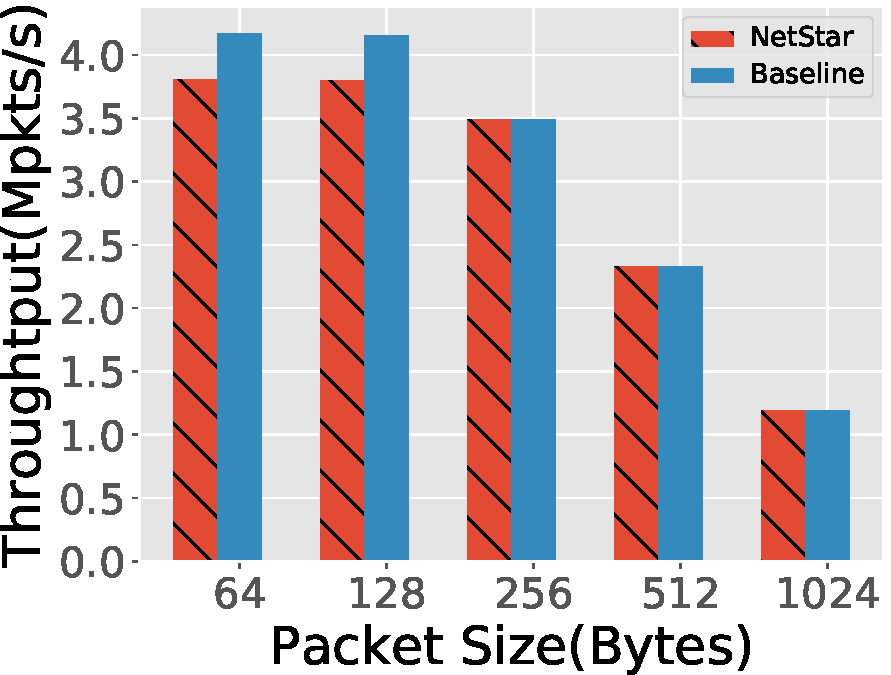
\includegraphics[width=\columnwidth]{chap-netstar/figure_src/Raw_forwarding_performance.pdf}
    \caption{}\label{fig:eval1.1}
  \end{subfigure}\hfill
  %\begin{subfigure}[t]{0.49\linewidth}
  %  \centering
  %  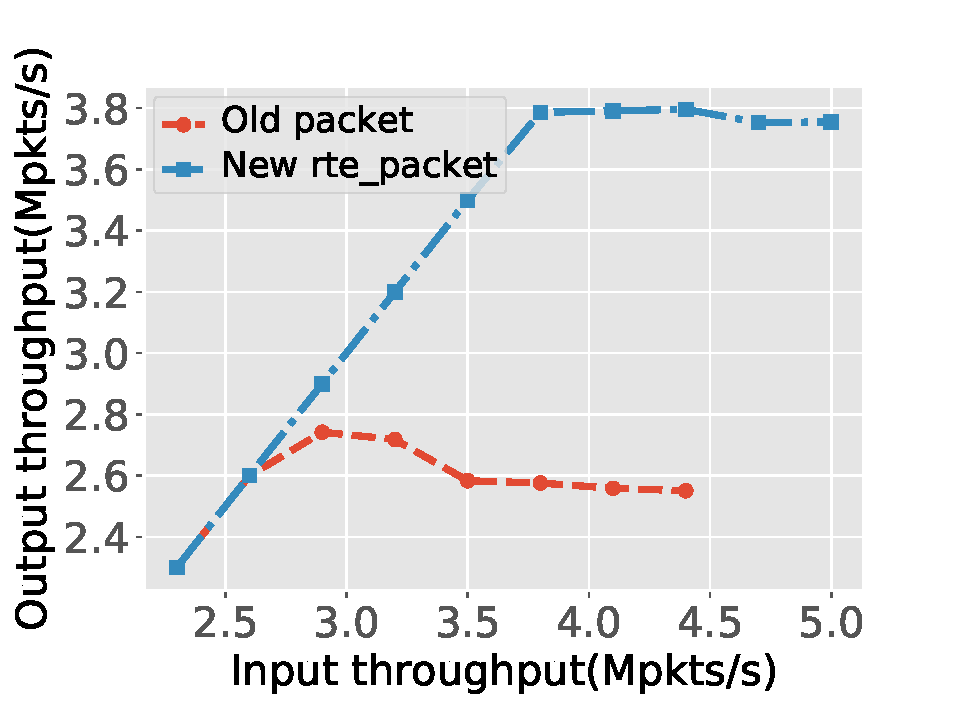
\includegraphics[width=\columnwidth]{figure_src/throughput_collapse.pdf}
  %  \caption{}\label{fig:eval1.2}
  %\end{subfigure}\hfill
  \begin{subfigure}[t]{0.49\linewidth}
    \centering
    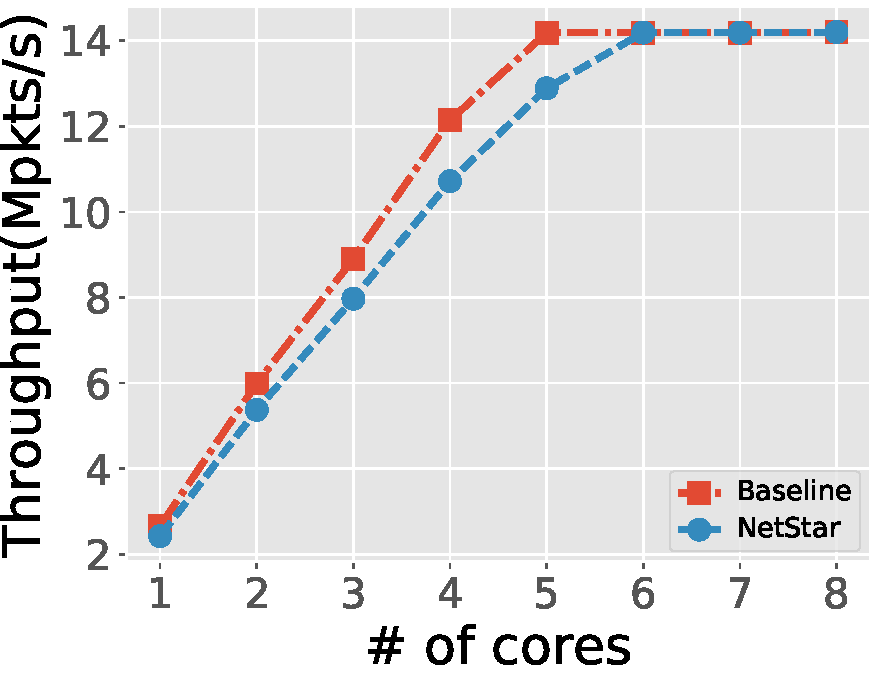
\includegraphics[width=\columnwidth]{chap-netstar/figure_src/scalability.pdf}
    \caption{}\label{fig:eval1.2}
  \end{subfigure}
\caption{Micro benchmarking on packet processing speed.}
\label{fig:eval1}
\end{figure}


To scale to line-rate processing when handling complex asynchronous operations, \netstar~should at least have adequate performance when being used as a simple packet forwarder. To evaluate this, we build a simple packet forwarder using \netstar, where the processing logic in each async-flow object is to directly forward all the received packets. For comparison, we also build a packet forwarder using DPDK \cite{dpdk}, which classifies packets into different flows by checking their flow-5-tuple against a cuckoo hash table adopted from the BESS virtual switch \cite{bess}, and passes packets belonging to a flow to its flow object for forwarding.
Compared with \netstar, the overhead associated with creating future object and chaining continuation functions are removed for the baseline forwarder, making it run faster. %To verify the effectiveness of our packet copy elimination optimization in Sec.~\ref{implementation}, we also show performance of a \netstar~version where fast packet optimization is disabled and the default Seastar handling is used.


Fig.~\ref{fig:eval1.1} shows packet processing throughput when the NFs are running on a single thread. 10000 UDP flows with different packet sizes are dispatched to an NF at the rate that is slightly larger than the maximum throughput achieved by the NF.
The throughput achieved by \netstar~is very close to the baseline. % when our optimization is in place. %Fig.~\ref{fig:eval1.1} also demonstrates the effectiveness of our fast packet optimization. We get an averaged 29\% throughput improvement over the unoptimized version.
%Fig.~\ref{fig:eval1.2} further shows the effectiveness of adopting our packet copy elimination in \netstar, when 10000 UDP flows with 64-byte packets are injected to the NF at gradually increasing packet rates.
%The generated traffic is sent to both the \netstar forwarder running on a single CPU core and an unoptimized forwarder. We measure the output packet rate and illustrate the result in . Besides improved performance,
 %It also ensures a more stable throughput even when the NF becomes overloaded. %According to Fig.~\ref{fig:eval1.2}, the unoptimized forwarder experience a 6\% throughput drop when overloaded while forwarder with fast packet optimization only experiences a 1\% throughput drop.
When each NF runs on multiple threads (CPU cores) and 100000 UDP flows with 64-byte packets at 10Gbps line rate are injected, Fig.~\ref{fig:eval1.2} shows that the throughput of \netstar~is always close to the baseline. With 6 cores, \netstar~achieves 10Gbps line rate. % input traffic consisting of 64 bytes small packets.
We evaluate \netstar~using small packets to better understand its packet forwarding performance, since larger packets are easier to saturate the NIC bandwidth, making NIC a bottleneck rather than revealing any performance bottleneck in our framework. We believe that the throughput of \netstar~can easily scale up to 40Gbps when it runs on a multi-core server and handles larger input packets.

%The core logic of the \netstar~forwarder is implemented with 75 LoC, whereas the baseline requires 93 LoC.

\subsubsection{Asynchronous Database Query}
\label{microbenchmark_db}

\begin{figure}[!h]
  \begin{subfigure}[t]{0.49\linewidth}
    \centering
    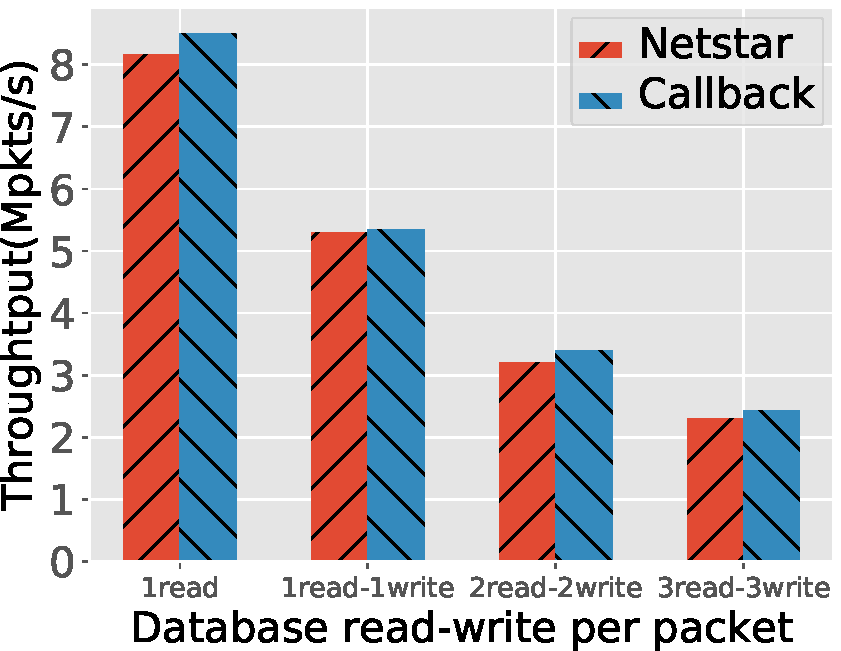
\includegraphics[width=\columnwidth]{chap-netstar/figure_src/read_write_throughput.pdf}
    \caption{}\label{fig:eval2.1}
  \end{subfigure}\hfill
  \begin{subfigure}[t]{0.49\linewidth}
    \centering
    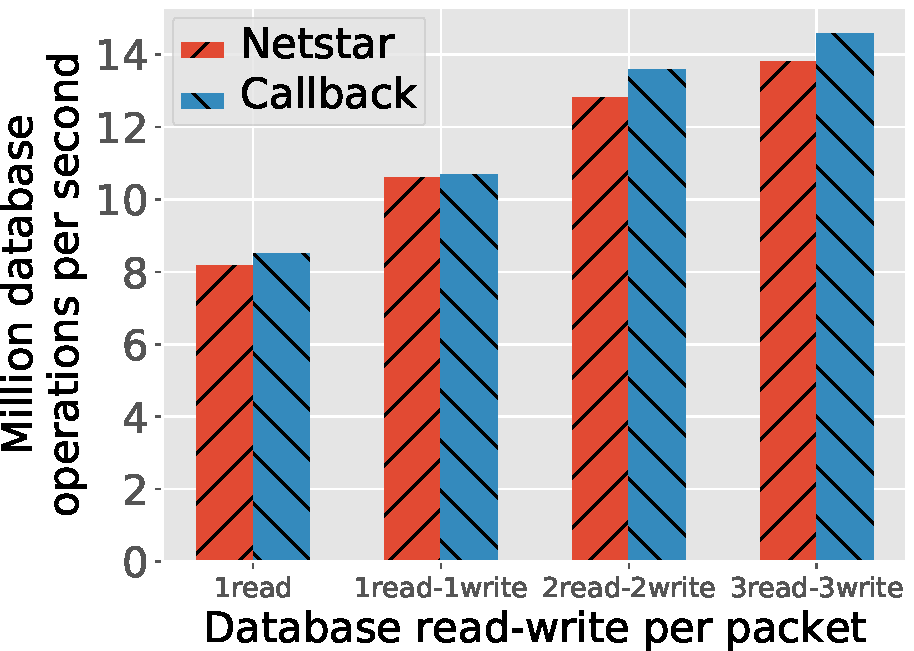
\includegraphics[width=\columnwidth]{chap-netstar/figure_src/read_write_speed.pdf}
    \caption{}\label{fig:eval2.2}
  \end{subfigure}
\caption{Micro benchmarking on asynchronous DB queries.}
\label{fig:eval2}
\end{figure}

We next develop a simple NF in which each async-flow object reads from and writes to a mica database as its core processing logic. Each write stores a key-value pair, where the key is the packet's flow-5-tuple and the value is a 24-byte random array. Each read retrieves a key-value pair using the packet's flow-5-tuple. We also implement the same NF functionality on a callback-based framework built on top of DPDK: a callback function is registered with each database query; when the database response arrives, the callback function is invoked to handle the response. Compared with the \netstar-based implementation, this framework imposes minimum runtime overhead when executing asynchronous operations: the registered callback is simply a function pointer without any heap allocation, whereas dynamic allocation and deallocation of future/promise object on the heap are involved in a future/promise-based framework.

%we vary the number of database queries that the async-flow object carries out per packet: from one read only, to one read-write, up to three consecutive read-write.
%The async-flow object may read-write the database multiple times and it only releases the received packet out when all the database queries finish.

We use 100000 UDP flows with 64-byte small packets at 10Gbps line rate. We vary the number of database read/write carried out by the NF when processing each packet. After receiving each packet, those read/write operations are consecutively carried out, before sending the packet out. Both \netstar~and the callback implementation run using 10 threads.
Fig~\ref{fig:eval2} shows that the packet processing throughput and the number of database queries that \netstar~can achieve is very close to that of the callback-based implementation. The average performance gap under various database access patterns is 4.23\% for packet throughput and 3.98\% for database operations per second.

%The core logic of the \netstar~implementation requires 54 LoC, whereas the baseline requires 80 LoC.
%Fig.~\ref{fig:eval2.2} shows that the \netstar can gradually increase the database query frequency if more database accesses are carried out for each processed packet. When the database is queries for 6 times to process a single packet, \netstar is capable of interacting with the database for over 13M times per second, while processing over 2M network packets.
%\chuan{give the LoC for each type of implementation}

\subsection{NFs from the StatelessNF paper\cite{201545}}
\label{sec:eval2}

\begin{figure}[!h]
  \begin{subfigure}[t]{0.49\linewidth}
    \centering
    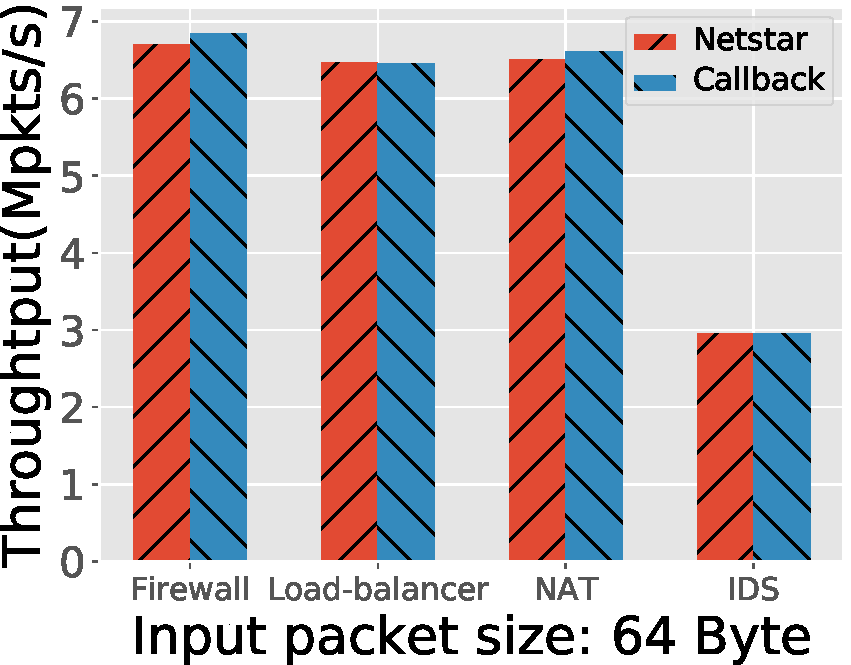
\includegraphics[width=\columnwidth]{chap-netstar/figure_src/StatelessNF_throughput_comparison_64byte.pdf}
    \caption{}\label{fig:eval3.1}
  \end{subfigure}\hfill
  \begin{subfigure}[t]{0.49\linewidth}
    \centering
    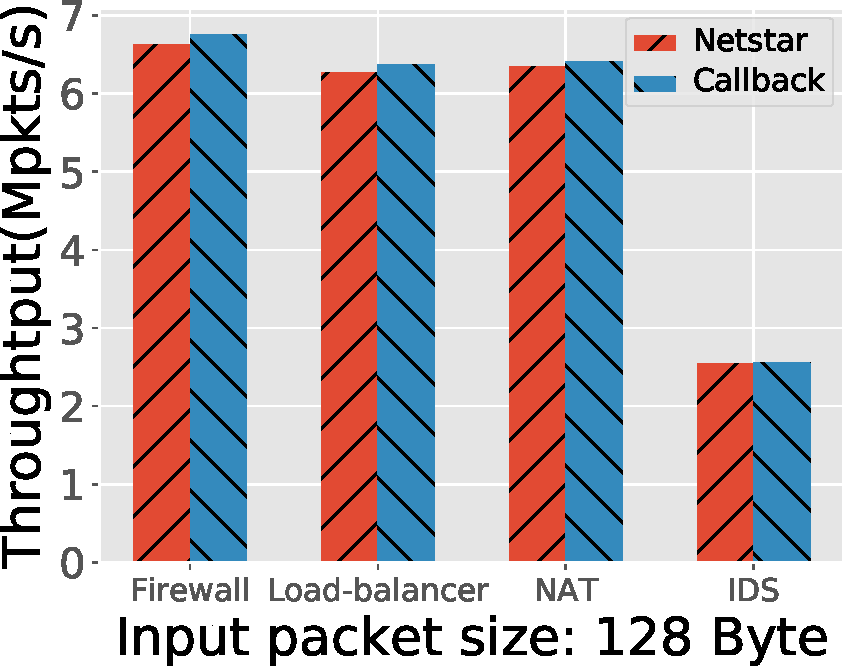
\includegraphics[width=\columnwidth]{chap-netstar/figure_src/StatelessNF_throughput_comparison_128byte.pdf}
    \caption{}\label{fig:eval3.2}
  \end{subfigure}\hfill
  \begin{subfigure}[t]{0.49\linewidth}
    \centering
    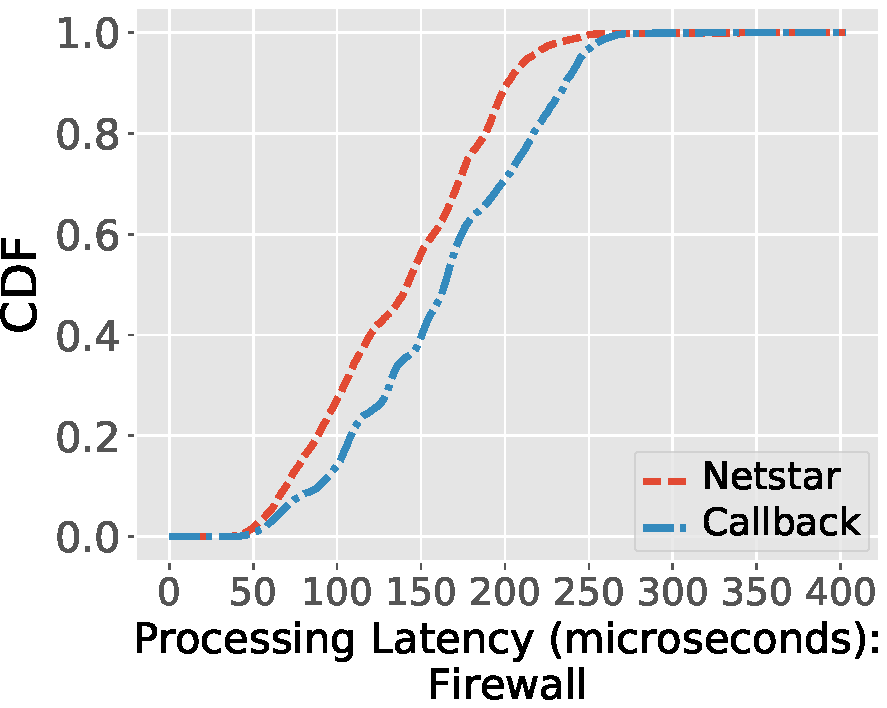
\includegraphics[width=\columnwidth]{chap-netstar/figure_src/firewall_throughput_latency_cdf.pdf}
    \caption{}\label{fig:eval3.3}
  \end{subfigure}\hfill
  \begin{subfigure}[t]{0.49\linewidth}
    \centering
    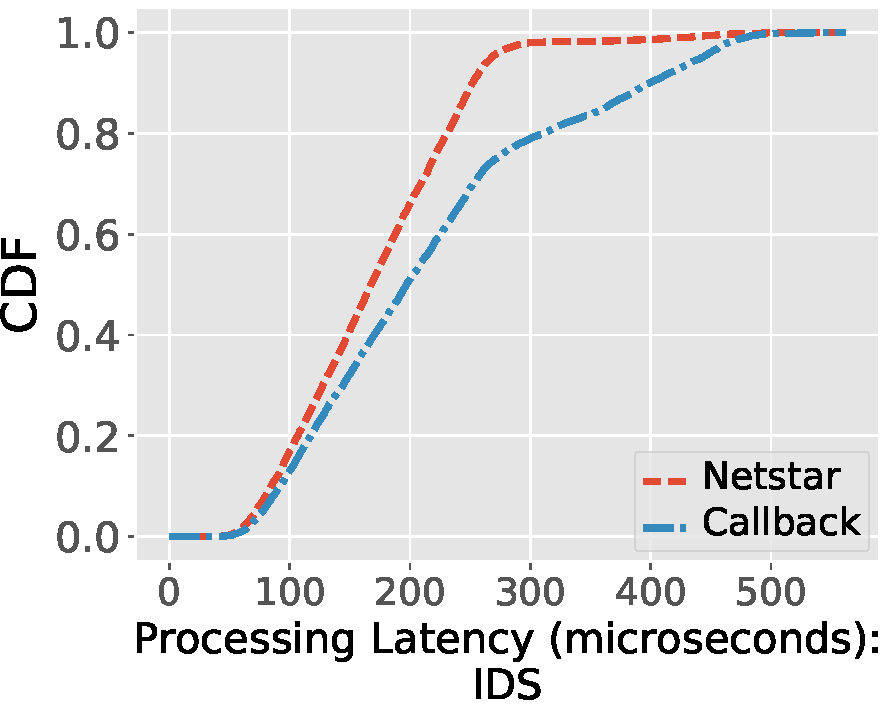
\includegraphics[width=\columnwidth]{chap-netstar/figure_src/ids_throughput_latency_cdf.pdf}
    \caption{}\label{fig:eval3.4}
  \end{subfigure}
\caption{Performance comparison: NFs from the StatelessNF paper.}
\label{fig:eval3}
\end{figure}


We compare our \netstar~based implementation of the four NFs with callback-based implementation (implemented following the pseudo-code logic), % using the callback-based framework as in Sec.~\ref{microbenchmark_db}),
as well as with the reported performance of NFs implemented by StatelessNF authors. We inject into each NF 100000 TCP flows at 10Gbps and vary the size of the flow packets. Each NF runs using 10 threads on a server, and accesses the mica database on a different server. % The NF reads and updates all the important per-flow state using the same procedure described in the StatelessNF paper.



%\noindent \textbf{A Callback-based Framework.}To evaluate the performance of \netstar framework, as well as comparing the implementation difficulty between future/promise abstraction and callback functions, we also implement the four NFs using a callback based framework. The callback based framework is implemented on top of DPDK for fast packet processing. To query mica database within this framework, the flow needs to register a callback function. When the database response arrives, the callback function is invoked to handle the response. Compared with \netstar, this framework imposes minimum runtime overhead when executing asynchronous operations: the registered callback function is simply a function pointer without any heap allocation, whereas future/promise abstraction needs to dynamically allocate and deallocate future/promise object on the heap.


In Fig.~\ref{fig:eval3.1} and Fig.~\ref{fig:eval3.2}, we observe that the packet processing throughput of our \netstar~NFs is very comparable with the callback-based NFs. % lower than 7M ppps for the firewall, NAT and load balancer. This is consistently with the evaluation result from Fig.~\ref{eval2.1}, as these three NFs only need to read the database once to process a single packet after the connection is established. The performance of IDS is smaller, due to the increased runtime overhead for passing the packet through AC automaton.
As compared to our observations in Sec.~\ref{microbenchmark_db}, when more complicated packet processing logic is involved here to process each packet besides executing asynchronous operations, the performance gap between \netstar~and the callback-based implementation decreases to only 2\%. We have also measured packet processing throughput when the packet size is 256, 512 or 1024 bytes. With a larger packet size, the NFs (except the IDS) can approach a 10Gbps processing rate. For IDS, the rate can reach 6.78 Gbps when processing 1024 bytes packets.

Fig.~\ref{fig:eval3.3} and Fig.~\ref{fig:eval3.4} show the CDF of packet processing latency at the firewall and the IDS when the packet size is 64 bytes. The packet processing latency between~\netstar~and the baseline is close to each other. %\netstar~achieves a smaller packet processing latency as the mica client library implemented in \netstar~has a more stable performance. %\chuan{give the reason}.

% We also compare throughout achieved by \netstar~NFs with reported performance in the StatelessNF paper. \netstar~can achieve over 6Mpps throughput on a single 10-core server (10 threads), while 4Mpps throughput is achieved in the paper using two 12-core servers.

%\subsubsection{Compare Implementation Difficulty.}

\begin{table}[!h]
\centering
\caption{LOC Comparison: NFs from the StatelessNF Paper}
\label{table:loc}
\resizebox{0.6\columnwidth}{!}{
\begin{tabular}{|l|l|l|l|}
\hline
   NF           & Callback  & \netstar  & Reduction \%\\ \hline
Firewall      & 52(44+8)  & 41(34+7) & 21.1\%        \\ \hline
Load balancer & 82(66+16) & 64(57+7) & 21.9\%        \\ \hline
NAT           & 99(79+20) & 80(73+7) & 19.1\%        \\ \hline
IDS           & 50(42+8)  & 43(36+7) & 14\%          \\ \hline
\end{tabular}
}
\vspace{-3mm}
\end{table}

To compare the implementation difficulty, we list the LOC for implementing the core processing logic of the four NFs using \netstar and the callback framework in Table~\ref{table:loc}. We only count the core processing code because a full-fledged implementation of each NF involves large volumes of auxiliary code on memory management, packet preprocessing and mica client library implementation. %All the four NFs require thousands lines of auxiliary code.
We can see that with the future/promise abstraction, the LOC can be reduced by as much as 21.9\%.
In the additions in Table~\ref{table:loc}, the number on the left is the total LOC for implementing packet processing functionalities, and the number on the right is the LOC for error handling. Due to consolidated error handling in \netstar, the same 7 lines of code are used for handling all errors in all NFs. %In the callback-based implementation,  requires defining redundant error handling logic in different callback functions. If the processing logic requires multiple asynchronous interactions with external services like the NAT, the redundant error handling logic may complicate the entire implementation.

\subsection{HTTP Reverse Proxy}
\label{sec:eval3}

\begin{figure}[!h]
  \begin{subfigure}[t]{0.49\linewidth}
    \centering
    \includegraphics[width=\columnwidth]{chap-netstar/figure_src/Proxy_throughput.pdf}
    \caption{}\label{fig:eval4.1}
  \end{subfigure}\hfill
  \begin{subfigure}[t]{0.49\linewidth}
    \centering
    \includegraphics[width=\columnwidth]{chap-netstar/figure_src/Proxy_RTT.pdf}
    \caption{}\label{fig:eval4.2}
  \end{subfigure}
\caption{Performance comparison: different proxies.}%HTTP request rate and HTTP transaction completion time for different proxies.}
\label{fig:eval4}
\end{figure}


We compare our proxy implemented using \netstar~with both HAProxy version 1.8 \cite{haproxy} and TinyProxy version 1.8.4 \cite{tinyproxy}.
TinyProxy does not use a callback-based asynchronous design; instead, it creates a new thread to handle each TCP flow in a synchronous manner, and relies on the kernel scheduler to schedule different threads. Each proxy runs on 10 threads. %We configure all the proxies to fully utilize all the 10 CPU cores of the server.
We use the HTTP benchmarking tool to generate 200 connections that go through the proxy, and then keeps producing HTTP requests at the generator's maximal capability. %The payload size of HTTP responses varies from 7 bytes to 32K bytes. %The HTTP request rate and the HTTP transaction completion time are both recorded.

In Fig.~\ref{fig:eval4.1}, we see that \netstar~out-performs HAProxy by up to 20\% and is better than TinyProxy much more. As the payload size of HTTP response increases, the consumed bandwidth on the NIC gradually reaches 10Gbps, making the NIC a bottleneck and hence decreasing the performance gap. %When the size of the HTTP response content is 7 bytes, \netstar out-perform HAProxy by almost 20\%. The performance difference gradually diminishes as the size of the HTTP response content increases.
Fig.~\ref{fig:eval4.2} shows that the smallest HTTP transaction completion time is achieved by \netstar.

Note that we implement our proxy by translating the processing logic in TinyProxy, as our future/promise based framework can easily mimic a synchronous execution flow. Such a translated \netstar~proxy is easy to implement, runs in full asynchrony and has superior performance even compared to HAProxy, as shown by the above results.

%\chuan{give LOC results of the three proxies} HAProxy and TinyProxy are open-source software, we didn't implement them, so it's better not to compare the LoC.

\subsection {IDS}
\label{sec:eval4}

\begin{figure}[!h]
  \begin{subfigure}[t]{0.45\linewidth}
    \centering
    \includegraphics[width=\columnwidth]{chap-netstar/figure_src/IDS_throughput.pdf}
    \caption{}\label{fig:eval5.1}
  \end{subfigure}\hfill
  \begin{subfigure}[t]{0.53\linewidth}
    \centering
    \includegraphics[width=\columnwidth]{chap-netstar/figure_src/IDS_RTT.pdf}
    \caption{}\label{fig:eval5.2}
  \end{subfigure}
\caption{Performance comparison: IDS.} %HTTP request rate and HTTP transaction completion time for IDSes implemented using \netstar and mOS.}
\label{fig:eval5}
\end{figure}

%\chuan{Fig.~\ref{fig:eval5}: change `HTTP response content size' to `HTTP response payload size'}

% To compare the performance of this IDS, we re-implement a similar IDS with mOS library \cite{}. We choose mOS because it is the state-of-art library implemented with callback-based event-driven style. We can use an implementation in mOS to evaluate whether NetStar approaches state-of-art performance.

We compare the IDS built with \netstar~and one built with mOS \cite{201546}, one of the fastest frameworks for building middleboxes that handle application-level payload reconstruction. mOS extensively uses the callback-based event-driven model. Our IDS implementation on mOS relies on registering various callback functions to the mOS framework to obtain reconstructed TCP byte stream and parsing HTTP request.
We generate 24K concurrent HTTP connections to pass through each IDS. %, then we measure the throughput and the HTTP transaction completion time achieved by the two IDSes.
The number of threads used by each IDSes varies, from 1 thread to 6 threads, to test the scalability.

In Fig.~\ref{fig:eval5}, we can see that the performance of \netstar~is very close to that achieved by the mOS-based implementation. %The highlight of \netstar is that the high-level programming environment it provides simplifies HTTP request parsing: after receiving a new piece of payload, we can convert the payload into an input stream and feed the input stream to an HTTP request parser provided in the Seastar framework, which is built with the REGAL library \cite{} and is robust to various parsing errors; then we can query from the parser whether we have received a complete HTTP request, and forward the entire HTTP request to the AC automaton for parsing. On contrary, the default HTTP request parser provided by mOS source code is rather simple. It only tries to inspect whether there contains special delimiter. This makes the HTTP request parser vulnerable to various parsing errors.
On the other hand, 493 LOC are written to implement the core processing logic in our \netstar~IDS, whereas 689 LOC are used in the mOS-based implementation, achieving a 28\% reduction.

\subsection {Malware Detector}
\label{sec:eval5}

\begin{table}[!h]
\centering
\caption{Performance of Malware Detectors}
\label{table:malware-detector-stat}
\resizebox{\columnwidth}{!}{
\begin{tabular}{|l|l|l|l|l|}
\hline
     & \begin{tabular}[c]{@{}l@{}}Throughput\\ (file size: 8k) \end{tabular} & \begin{tabular}[c]{@{}l@{}}Throughput\\ (file size: 32k) \end{tabular} & \begin{tabular}[c]{@{}l@{}}HTTP transaction\\ completion time \\(file size: 8k) \end{tabular} & \begin{tabular}[c]{@{}l@{}}HTTP transaction\\ completion time \\(file size: 32k) \end{tabular} \\ \hline
\begin{tabular}[c]{@{}l@{}}Asynchronous \\ Malware Detector\end{tabular} & 5.02 Gbps                                                              & 6.19 Gbps                                                                & 12.74 ms                                                                                    & 41.33 ms                                                                                     \\ \hline
\begin{tabular}[c]{@{}l@{}}Local Malware\\ Detector\end{tabular}         & 5.86 Gbps                                                               & 6.79 Gbps                                                                & 10.77 ms                                                                                   & 37.84 ms                                                                                     \\ \hline
\end{tabular}
}
\vspace{-5mm}
\end{table}

We compare our asynchronous malware detector that queries an external database and a DNS server (run in the same cluster as the malware detector) with a local malware detector that only tries to identify if the file hash exists in a local in-memory malware hash table. Both malware detectors are implemented using \netstar.
We generate 1000 HTTP connections and send files in these HTTP connections from the client to the server. We randomly populate the content of the file with malware. The size of the files vary from 8K bytes to 32K bytes. Both malware detectors run using one thread.% without multi-core scaling.

In Table~\ref{table:malware-detector-stat}, % shows the throughput and average HTTP transaction completion time achieved by both malware detectors.
 we can see that compared with a local version, the asynchronous malware detector experiences a 14\% throughput drop when the size of the transmitted file is 8K and 8.8\% throughput drop when the size of the transmitted file is 32K. The remote malware detection process adds a 1.97ms/3.48ms latency respectively. %Throughout the evaluation, all the generated malwares are successfully detected.

We purposely compare a malware detector accessing external services with a local malware detector, instead of a callback-based malware detector which also accesses external services, in order to show the following: our NF's performance is very comparable with a fast local detector, not to mention one accessing external services; with \netstar, complicated asynchronous operations can be enabled on NFs without large performance drop, and the future/promise abstraction provided by \netstar~enables easy implementation of the asynchronous operations.

\subsection{Comparison with Coroutine}
\label{sec:eval6}

Finally, we compare \netstar~with a coroutine based NF framework. %For \netstar, we reuse the NFs for querying the database as shown in~Sec.~\ref{}.
In the coroutine framework, for each new flow, a new coroutine (thread) is created and a similar packet processing loop as in our async-flow object runs within the coroutine. Whenever a coroutine needs to waits for an asynchronous event, it yields its control to other coroutines in the NF. %We directly utilize the coroutine module in Seastar to implement the coroutine framework.

We compare the \netstar~NF carrying out database queries in Sec.~\ref{microbenchmark_db} with a coroutine based implementation. 10000 UDP flows are sent to the two NFs, both running in one thread. Each NF reads the database once when processing one packet. A 750K pps throughput is achieved by the NF implemented with \netstar, while the throughput of the coroutine-based NF is only 147K pps. Further profiling reveals that the average coroutine switching time is around 352 nanoseconds. Even though the time is small, constant coroutine switching adds considerable overhead when an NF processes a large number of flows. %The constant coroutine switching adds considerable overheads to packet processing.
Therefore, coroutine is a less desirable paradigm for implementing asynchronous NFs when compared with the future/promise abstraction.

\section{Discussions}

In our current \netstar~implementation, after issuing an asynchronous operation, an async-flow object waits for the asynchronous operation to complete, while \netstar~runs other async-flow objects. During this time, new flow packets coming to this async-flow object are buffered in its FIFO queue. This design choice is consistent with the semantics in most NFs, which requires processing packets in a flow strictly in sequence, and moving on to process the next packet only when all the processing on the current packet is completed. On the other hand, some NFs may carry out other asynchronous operations besides packet processing, \eg, writing logs into external storage. Such an extra operation can be done concurrently with packet processing. To handle this case,
we can launch a stand-alone asynchronous operation from the core NF processing logic and obtain a returned future object. As long as we do not add this future object into the ``future-continuation'' chain that leads to the creation of \lstinline[style=InlineStyle]{future<action>} in Fig~\ref{fig:simulated_loop}, the async-flow object will not wait for the completion of this stand-alone asynchronous operation and it proceeds with packet handling concurrently.
%we can easily revise our async-flow object design slightly, such that it does not wait for the completion of an asynchronous packet processing operation, but handles the extra operations first (which are also handled in future objects) as follows: we do not allow the future object handling the packet processing operation to return a future<action>, and then the async-flow object will not wait for the completion of this operation, but moves on to other operations.\chuan{check if the above descriptions are accurate}


We have shown that using the future/promise paradigm can simplify asynchronous programming. Learning to use the future/promise abstraction may take some efforts, which makes use of various advanced C++14 features including move semantics, lambda functions and template meta programming. Our own experience is that, once a programmer has spent some time getting familiar with the future/promise abstraction, he can greatly improve his productivity when programming asynchronous code.

In addition, porting existing NF code to our \netstar~framework is feasible, but may require some extra efforts on converting the callback-based programming interfaces to the future/promise abstraction, which usually involves exposing a new interface that returns a future object containing an asynchronous response. Once  the concept of future/promise is mastered, this process can be made relatively easy.

%We have not experienced porting existing NF code to \netstar, but we do port the mica client interface code to \netstar so that our NFs can access mica database. The major effort is  on converting the callback-based query interface to a future/promise based interface.

%Since Seastar provides several basic data structures that expose a future/promise based interface for porting existing software, this process is relatively easy. \chuan{add more explanations}% and can be done within a few days.


% In case that the async-flow object does not want to wait for the asynchronous operation to complete, like asynchronous logging, the async-flow object can directly issue an isolated asynchronous operation without chaining continuation function to the returned future, the Seastar scheduler can schedule these operations to run concurrently in an asynchronous fashion.

\section{Related Work}

%\noindent \textbf{Advanced Programming Frameworks for NFs.}
NetBricks proposes a fast and secure framework based on the Rust \cite{199352} language for building NFs. %NetBricks provides a high-level abstraction for building fast packet processing pipelines, but it does not address how to simplify asynchronous programming in NFs.
\netstar~leverages future/promise abstraction to process dataplane traffic, and simplifies asynchronous programming with the async-flow interface.
P4 \cite{bosshart2014p4} provides a high-level programming language for describing dataplane packet processing pipelines, but it has no intrinsic support for manipulating dataplane packets asynchronously as in \netstar. The BESS virtual switch \cite{bess} and the Click software router \cite{kohler2000click} share a similar design philosophy, which is to construct NFs by concatenating multiple simpler processing modules. It is possible to integrate callback-based asynchronous interfaces into both BESS and Click to handle dataplane packets asynchronously, but implementation effort would be more significant than in \netstar, due to the inherent limitation of callback functions when compared with future/promise abstraction.
mOS \cite{201546} proposes a unified interface for managing connection oriented middleboxes. Using its interface, a middlebox can extract application-level payload and apply different callback functions to process the payload. \netstar~shares a similar event layer as in mOS, where the packet is preprocessed to expose interested events to the core NF processing logic; however, \netstar~uses the future/promise abstraction for event handling, and can effectively simplify implementation in case the NF requires to contact external services.

%\noindent \textbf{NFs with Asynchronous Operations.}
%The trend of NFV adds more requirement to NFs.
Except for being fast, NFs should be designed to resist various failures and handle large workload. %work in a large cluster.
StatelessNF \cite{201545} proposes a new architecture that separates the storage of per-flow states from the processing of packets. This advanced architecture requires efficient and simplified asynchronous programming support, which is nicely provided by \netstar. OpenNF \cite{gember2015opennf}, Split/Merge \cite{rajagopalan2013split} and PEPC \cite{Qazi:2017:HPP:3098822.3098848} all use flow migration for dynamical scaling of NF instances (by migrating flows out of hotspots). Implementation of a flow migration protocol typically involves complex asynchronous interactions, and \netstar~can be potentially useful to simplify flow migration implementation.

%\chuan{most discussions in the following duplicate with what was introduced earlier in the paper. Comment out this paragraph and you can move necessary introduction to future/promise, Seaster to earlier part of the paper}
%\noindent \textbf{The History of Future/Promise Abstraction.} The history of future/promise abstraction dates back to 1980s \cite{}. Over the years, the implementation technique of future/promise abstraction has evolved a lot, but most implementation appears in high-level functional programming languages like OCaml \cite{} and Haskell \cite{}, limiting its applicability to dataplane packet processing. The future/promise abstraction used in this paper belongs to a special monadic structure, which is first proposed by ...\cite{}. ... \cite{} and ...\cite{} implement such a future/promise abstraction in OCaml and Haskell, respectively. Recently, Seastar \cite{} implements a fast future/promise abstraction using C++, paving the way for applying it to dataplane packet processing. Besides C++, Rust programming language \cite{} also has a fast future/promise abstraction implementation \cite{}, it is possible to port NetStar to Rust to enjoy a safe execution environment, but it is beyond the scope of this paper.

\section{Conclusion}

This paper proposes \netstar, the first attempt to bring the future/promise abstraction to the NF dataplane for flow processing.  \netstar~adopts a dual-stack approach, enabling it to implement NFs processing packets at different layers. To fully utilize the power of future/promise, we carefully design an async-flow interface that chains a number of future/promise and continuation functions for efficiently handling a series of asynchronous operations. Using \netstar, asynchronous programming in NFs is made easy, elegant, while good packet processing performance is still guaranteed. Our extensive evaluation shows that \netstar~can effectively simplify asynchronous programming asynchronous in NFs, while easily achieve line-rate packet processing for NFs.


\chapter {Conclusion and Future Work}
\label{ch:conclusion}
\lhead{\chaptername \ \ref{ch:conclusion}.\ \emph{Conclusion and Future Work}} %

\section {Concluding Remarks}

This thesis discusses the design and implementation of \textit{ScalIMS}, \nfactor~and \netstar, which improve the scalability, performance of resilience functionalities and programability over existing NFV systems altogether.

\textit{ScalIMS} scales control-plane and data-plane service chains of IMS systems across geo-distributed datacenters by combining the benefits of proactive and reactive scaling. Evaluation of our prototype implementation on IBM SoftLayer cloud shows that \textit{ScalIMS} effectively reduces the total number of provisioned VNF instances while guaranteeing good traffic QoS.

\nfactor~leverages actor model to achieve transparent and highly efficient resilience functionalities. Our experiments show that \nfactor~achieves good scalability and high packet processing speed, as well as fast flow migration and failure recovery.

\netstar~represents first attempt to bring the future/promise abstraction to the NF dataplane for flow processing. Using \netstar, asynchronous programming in NFs is made easy and elegant, while good packet processing performance is still guaranteed. Our extensive evaluation shows that \netstar~can effectively simplify asynchronous programming asynchronous in NFs, and easily achieve line-rate packet processing for NFs.

\section {Future Work}

We identify two important research directions that are inspired by the study of this thesis.

\subsection{Bring Paxos-based Fault-tolerance to NFV}

An important application of both \nfactor~and \netstar~is to make NFs fault-tolerant. \nfactor~achieves fault-tolerance by constantly check-pointing the per-flow state of a flow actor to an replica actor, while \netstar~resists to failures by saving and updating important per-flow state to an external in-memory storage system.

Even though both methods can improve the failure-resilience performance of NFV system, they can only tolerate the failure of the NF instance that is correctly replicated. In practice, it is possible for both the replicated NF instance and the replica for storing important NF states to fail concurrently. In that case, the replicated NF will never be correctly recovered due to the loss of important NF states from the replica.

An important method for fighting against concurrent failures is to run Paxos algorithm \cite{lamport1998part}. With Paxos, a cluster of server instances can form a consensus group and the cluster can tolerate $N/2$ failured server instances for all $N$ server instances existed in the cluster. Existing work, like Crane \cite{cui2015p}, has discussed replicating general-purpose server system using Paxos algorithm.

However, replicating NF instances using Paxos algorithm raises a unique challenge over replicating general-purpose servers. NFs are usually design to work with a high input packet rate. A typical NF usually needs to process several million packets for each second. Such a high input rate poses a challenge for existing Paxos systems \cite{poke2015dare, 199299}, as they do not support such a high throughput.

Our work on \netstar~raises potential opportunities for bringing Paxos-based fault-tolerance to NFs. Implementing high-performance Paxos algorithm requires non-trivial asynchronous programming. With \netstar, we believe that the implementation of a Paxos replication system can be significantly simplified, while guaranteeing good performance. But to build a practical Paxos replication system for NFs, we still need to search for both architectural and algorithmic breakthroughs for Paxos algorithm.

\subsection{Building Formally Verified NFs}

An important research motivation for this thesis is to leverage modern programming paradigms to improve NFV system. In particular, this thesis discusses how to apply actor model and future/promise paradigm to improve the performance of resilience functionalities and the programability of high-performance NFs with asynchronous operations. Besides these two programming paradigms, another important paradigm which is worth further exploration is formal verification.

Building formally verified system software has draw important research attention in recent years \cite{199344, nelson2017hyperkernel, zaostrovnykh2017formally}. Formally verified software provides the strongest guarantee against various kinds of bugs and security risks. We believe that formal verification is extremely important for NFV technology as well. NFs are important access gateways of the underlying service, therefore any bugs and security risks of the NF may render the entire service protected by the NF useless.

A recent break-through in the formal verification of NFs is VigNAT \cite{zaostrovnykh2017formally}. VigNAT combines model-checking with theorem proving: it uses model-checking to check stateless part of VigNAT, and relies on theorem proving to verify the correctness of important data-structures used by VigNAT. By combining the result of model-checking and theorem proving, the VigNAT obtains a completely verified NF.

There are two major problems associated with VigNAT. First, VigorNAT treats the entire DPDK library \cite{dpdk} as the trusted computing base. VigorNAT assumes that DPDK is correct and does not care about potential bugs in DPDK library. However, DPDK itself is an extremely complicated library. It is used to retrieve network packets from the NIC card and serves as the the core of many modern, high-performance NFs. To further improve the reliability of formally verified NFs, the DPDK library must be removed from the trusted computing base. Second, the verification of the data-structures used by VigNAT only preserves the correctness up to the semantics of C programming language. There is no guarantee that the compiled machine code is correct.

We believe that to further improve the reliability of formally verified NFs, an effective approach is to adopt recent advancement of formal verification techniques, especially the Verified Software Toolchain (VST) project \cite{vst}. The VST project applies formal verification directly to C code, and guarantees the correctness of the compiled machine code with the help of CompCert compiler \cite{leroy2006formal}. Also, a recent project called ixy \cite{ixy} demonstrates the implementation of a simple user-space packet processing library, whose functionality is similar to DPDK. By following the design approach of ixy, it is possible to build a formally verified user-space packet processing library and remove DPDK library from the trusted computing base.

%Implementing high-performance Paxos algorithm inside NFs requires non-trivial asynchronous programming, which

%\chapter{Related Work}

adfsfd \cite{carpentier2014extreme}.


%\input{Chapter1} %introduction

%\input{Chapter2} %related work

%\input{Chapter3} %work 1

%\input{Chapter4} %work 2

%\input{Chapter5} %conclusion

%\input{Chapters/Chapter1-Introduction} % Introduction

%\input{Chapters/Chapter2-Smark-Subtitle} % work 1

%\input{Chapters/Chapter3-Speaker-Naming} % work 2

%\input{Chapters/Chapter4-Applications}   % applications

%\input{Chapters/Chapter5-Conclusion} % Conclusion

%% ----------------------------------------------------------------
% Now begin the Appendices, including them as separate files

\addtocontents{toc}{\vspace{2em}} % Add a gap in the Contents, for aesthetics

\appendix % Cue to tell LaTeX that the following 'chapters' are Appendices
% Appendix Title

%\input{Appendices/AppendixB} % Appendix Title

%\input{Appendices/AppendixC} % Appendix Title

\addtocontents{toc}{\vspace{2em}}  % Add a gap in the Contents, for aesthetics
\backmatter

%% ----------------------------------------------------------------
\label{Bibliography}
\lhead{\emph{Bibliography}}  % Change the left side page header to "Bibliography"
%\bibliographystyle{unsrtnat}  % Use the "unsrtnat" BibTeX style for formatting the Bibliography
\bibliographystyle{plain}    %  abbrv, acm, alpha, apalike, ieeetr, plain, siam or unsrt
\bibliography{egbibsample}  % The references (bibliography) information are stored in the file named "Bibliography.bib"

\end{document}  % The End
%% ----------------------------------------------------------------
